\DocumentMetadata{%
 %  uncompress, %only for debugging!!
  pdfversion=2.0,
  testphase={phase-II, tabular, graphic}%
 % testphase={phase-II,math, tabular, graphic}% TOC Does not work
   % testphase={phase-III,math}% TOC works
}
\tagpdfsetup{activate, tabsorder=structure}
% Use the following to fix bug in November 2023 download of LaTeX
\ExplSyntaxOn
\cs_generate_variant:Nn\__tag_prop_gput:Nnn{cnx}
\ExplSyntaxOff
\documentclass[11pt,
  english,
  letterpaper,
]{article}
\usepackage{sa4ss}
\usepackage{amsmath,amssymb,array}
\usepackage{booktabs}

% From tagged-template.latex
\usepackage{lmodern}
\usepackage{ifxetex,ifluatex}
\ifnum 0\ifxetex 1\fi\ifluatex 1\fi=0 % if pdftex
  \usepackage[T1]{fontenc}
  \usepackage[utf8]{inputenc}
  \usepackage{textcomp} % provide euro and other symbols
\else % if luatex or xetex
  \usepackage{unicode-math}
  \defaultfontfeatures{Scale=MatchLowercase}
  \defaultfontfeatures[\rmfamily]{Ligatures=TeX,Scale=1}
\fi

% Use upquote if available, for straight quotes in verbatim environments
\IfFileExists{upquote.sty}{\usepackage{upquote}}{}
\IfFileExists{microtype.sty}{% use microtype if available
  \usepackage[]{microtype}
  \UseMicrotypeSet[protrusion]{basicmath} % disable protrusion for tt fonts
}{}
\makeatletter
\@ifundefined{KOMAClassName}{% if non-KOMA class
  \IfFileExists{parskip.sty}{%
    \usepackage{parskip}
  }{% else
    \setlength{\parindent}{0pt}
    \setlength{\parskip}{6pt plus 2pt minus 1pt}}
}{% if KOMA class
  \KOMAoptions{parskip=half}}
\makeatother
\usepackage{xcolor}
\IfFileExists{xurl.sty}{\usepackage{xurl}}{} % add URL line breaks if available
\hypersetup{
  pdftitle={Status of copper rockfish (Sebastes caurinus) along the U.S. California coast south of Point Conception in 2023},
  pdflang={en},
  hidelinks,
  pdfcreator={LaTeX via pandoc}}
\urlstyle{same} % disable monospaced font for URLs
\usepackage{longtable}
% Correct order of tables after \paragraph or \subparagraph
\usepackage{etoolbox}
\makeatletter
\patchcmd\longtable{\par}{\if@noskipsec\mbox{}\fi\par}{}{}
\makeatother
% Allow footnotes in longtable head/foot
\IfFileExists{footnotehyper.sty}{\usepackage{footnotehyper}}{\usepackage{footnote}}
\makesavenoteenv{longtable}
\usepackage{graphicx}
\makeatletter
\def\maxwidth{\ifdim\Gin@nat@width>\linewidth\linewidth\else\Gin@nat@width\fi}
\def\maxheight{\ifdim\Gin@nat@height>\textheight\textheight\else\Gin@nat@height\fi}
\makeatother
% Scale images if necessary, so that they will not overflow the page
% margins by default, and it is still possible to overwrite the defaults
% using explicit options in \includegraphics[width, height, ...]{}
\setkeys{Gin}{width=\maxwidth,height=\maxheight,keepaspectratio}
% Set default figure placement to htbp
\makeatletter
\def\fps@figure{htbp}
\makeatother
\setlength{\emergencystretch}{3em} % prevent overfull lines
\providecommand{\tightlist}{%
  \setlength{\itemsep}{0pt}\setlength{\parskip}{0pt}}
\setcounter{secnumdepth}{5}
\usepackage{lineno}
\usepackage[inline]{showlabels}
\ifxetex
  % Load polyglossia as late as possible: uses bidi with RTL langages (e.g. Hebrew, Arabic)
  \usepackage{polyglossia}
  \setmainlanguage[]{}
\else
  \usepackage[shorthands=off,main=english]{babel}
\fi

%Define cslreferences environment, required by pandoc 2.8
%https://github.com/rstudio/rmarkdown/issues/1649
\newlength{\csllabelwidth}
\setlength{\csllabelwidth}{3em}
\newlength{\cslhangindent}
\setlength{\cslhangindent}{1.5em}
% for Pandoc 2.8 to 2.10.1
\newenvironment{cslreferences}%
  {}%
  {\par}
% For Pandoc 2.11+
\newenvironment{CSLReferences}[2] % #1 hanging-ident, #2 entry spacing
 {% don't indent paragraphs
  \setlength{\parindent}{0pt}
  % turn on hanging indent if param 1 is 1
  \ifodd #1 \everypar{\setlength{\hangindent}{\cslhangindent}}\ignorespaces\fi
  % set entry spacing
  \ifnum #2 > 0
  \setlength{\parskip}{#2\baselineskip}
  \fi
 }%
 {}
\usepackage{calc}  % for \widthof, \maxof in minipage
\newcommand{\CSLBlock}[1]{#1\hfill\break}
\newcommand{\CSLLeftMargin}[1]{\parbox[t]{\csllabelwidth}{#1}}
\newcommand{\CSLRightInline}[1]{\parbox[t]{\linewidth - \csllabelwidth}{#1}\break}
\newcommand{\CSLIndent}[1]{\hspace{\cslhangindent}#1}


\providecommand{\tightlist}{%
  \setlength{\itemsep}{0pt}\setlength{\parskip}{0pt}}

\usepackage{lineno}
\usepackage[inline]{showlabels}
\date{}
\newcommand{\trTitle}{Status of copper rockfish (\emph{Sebastes caurinus}) along the U.S. California coast south of Point Conception in 2023}
\newcommand{\trYear}{2023}
\newcommand{\trMonth}{May}
\newcommand{\trAuthsLong}{truetruetrue}
\newcommand{\trAuthsBack}{Wetzel, C.R., M.H. Monk, J. Coates}
\newcommand{\trCitation}{
\begin{hangparas}{1em}{1}
\trAuthsBack{}. \trYear{}. \trTitle{}. \glsentrylong{pfmc}, Portland, Oregon. \pageref{LastPage}{}\,p.
\end{hangparas}}

\newcommand\includegraphicsifexists[2][width=\linewidth]{\IfFileExists{#2}{\includegraphics[#1]{#2}}{}}

\begin{document}

%%%%% Frontmatter %%%%%

% Footnote symbols in front matter
\renewcommand*{\thefootnote}{\fnsymbol{footnote}}

\small
\thispagestyle{empty}
\pagenumbering{roman}
\noindent
\begin{center}
\title{Status of copper rockfish (\emph{Sebastes caurinus}) along the U.S. California coast south of Point Conception in 2023}
% \textnormal{\MakeTextUppercase{\trTitle{}}}
\vspace{1.5cm}
{\Large\textbf\newline{Status of copper rockfish (\emph{Sebastes caurinus}) along the U.S. California coast south of Point Conception in 2023}}

\includegraphicsifexists[width=4in]{figure_title.png}
\vfill
by\\
Chantel R. Wetzel\textsuperscript{1}\\
Melissa H. Monk\textsuperscript{2}\\
Julia Coates\textsuperscript{3}\vfill
\textsuperscript{1}Northwest Fisheries Science Center, U.S. Department of Commerce, National Oceanic and Atmospheric Administration, National Marine Fisheries Service, 2725 Montlake Boulevard East, Seattle, Washington 98112\\
\textsuperscript{2}Southwest Fisheries Science Center, U.S. Department of Commerce, National Oceanic and Atmospheric Administration, National Marine Fisheries Service, 110 McAllister Way, Santa Cruz, California 95060\\
\textsuperscript{3}.na.character\vfill
\trMonth{} \trYear{}
\end{center}
\clearpage

% Fourth page: Colophon
\thispagestyle{empty}
\vspace*{\fill}
\begin{center}
\copyright{} \glsentrylong{pfmc}, \trYear{}\\
\end{center}
\par
\bigskip
\noindent
Correct citation for this publication:
\bigskip
\par
\trCitation{}
\clearpage

% Add TOC to pdf bookmarks (clickable pdf)
\pdfbookmark[1]{\contentsname}{toc}

% Table of contents page, lists of figures and tables
\tableofcontents\clearpage
\label{TRlastRoman}
\clearpage

% Table of contents
\newpage
\thispagestyle{empty} % to remove page number

% Settings for the main document
\pagenumbering{arabic}  % Regular page numbers
\pagestyle{plain}  % No page number on first page of main document, use 'empty'
\renewcommand*{\thefootnote}{\arabic{footnote}}  % Back to numeric footnotes
\setcounter{footnote}{0}  % And start at 1
\renewcommand{\headrulewidth}{0.5pt}
\renewcommand{\footrulewidth}{0.5pt}
%\pagestyle{fancy}\fancyhead[c]{Draft: Do not cite or circulate}

\newcommand{\lt}{\ensuremath <}
\newcommand{\gt}{\ensuremath >}

\linenumbers

\newcommand\CapeM{$40^\circ 10^\prime N$}
\newcommand\PtC{$34^\circ 27^\prime N$}
\newcommand\CAOR{$42^\circ 00^\prime N$}

\pagebreak
\pagenumbering{roman}
\setcounter{page}{1}

\renewcommand{\thetable}{\roman{table}}
\renewcommand{\thefigure}{\roman{figure}}

\setlength\parskip{0.5em plus 0.1em minus 0.2em}

\vspace{500cm}

\hypertarget{disclaimer}{%
\section*{Disclaimer}\label{disclaimer}}
\addcontentsline{toc}{section}{Disclaimer}

\emph{\textbf{These materials do not constitute a formal publication and are for information only. They are in a pre-review, pre-decisional state and should not be formally cited or reproduced. They are to be considered provisional and do not represent any determination or policy of NOAA or the Department of Commerce.}}

\pagebreak

\hypertarget{executive-summary}{%
\section*{Executive summary}\label{executive-summary}}
\addcontentsline{toc}{section}{Executive summary}

\hypertarget{stock}{%
\subsection*{Stock}\label{stock}}
\addcontentsline{toc}{subsection}{Stock}

This assessment reports the status of copper rockfish (\emph{Sebastes caurinus}) off the California coast in U.S. waters, using data through 2022. The copper rockfish stock was assessed using two sub-area models that captured distinct inter-stock dynamics split north and south of Point Conception. The estimated dynamics for each assessed sub-area is described here along with the combined stock status for the California stock. This assessment does not account for populations located in Mexico waters or other areas off the U.S. coast and assumes that these southern and northern populations do not contribute to the population being assessed here.

\hypertarget{catches}{%
\subsection*{Catches}\label{catches}}
\addcontentsline{toc}{subsection}{Catches}

Replace text with trends and current levels. Include Table for last 10 years. Include Figure with long-term estimates.

\begingroup\fontsize{10}{12}\selectfont
\begingroup\fontsize{10}{12}\selectfont

\begin{longtable}[t]{r>{\centering\arraybackslash}p{1.83cm}>{\centering\arraybackslash}p{1.83cm}>{\centering\arraybackslash}p{1.83cm}>{\centering\arraybackslash}p{1.83cm}>{\centering\arraybackslash}p{1.83cm}}
\caption{\label{tab:south-removalsES}Recent catch by fleet and total catch summed across fleets for the sub-area model south of Point Conception.}\\
\toprule
Year & Commercial dead & Commercial live & Rec CPFV & Rec Private & Total Catch\\
\midrule
\endfirsthead
\caption[]{Recent catch by fleet and total catch summed across fleets for the sub-area model south of Point Conception. \textit{(continued)}}\\
\toprule
Year & Commercial dead & Commercial live & Rec CPFV & Rec Private & Total Catch\\
\midrule
\endhead

\endfoot
\bottomrule
\endlastfoot
2013 & 1.26 & 2.67 & 61.65 & 13.96 & 79.54\\
2014 & 1.79 & 2.29 & 47.58 & 10.04 & 61.71\\
2015 & 2.11 & 4.09 & 67.00 & 8.97 & 82.18\\
2016 & 2.11 & 3.57 & 82.20 & 11.07 & 98.95\\
2017 & 1.74 & 2.82 & 70.58 & 11.72 & 86.86\\
2018 & 2.93 & 2.20 & 81.97 & 14.21 & 101.31\\
2019 & 2.71 & 3.08 & 60.25 & 14.66 & 80.70\\
2020 & 3.54 & 3.58 & 56.39 & 23.01 & 86.52\\
2021 & 2.74 & 1.94 & 44.25 & 8.28 & 57.20\\
2022 & 0.69 & 0.21 & 14.12 & 4.50 & 19.52\\*
\end{longtable}
\endgroup{}
\endgroup{}


\begingroup\fontsize{10}{12}\selectfont
\begingroup\fontsize{10}{12}\selectfont

\begin{table}[t]{r>{\centering\arraybackslash}p{1.83cm}>{\centering\arraybackslash}p{1.83cm}>{\centering\arraybackslash}p{1.83cm}>{\centering\arraybackslash}p{1.83cm}>{\centering\arraybackslash}p{1.83cm}}
\caption{\label{tab:north-removalsES}Recent catches (mt) by fleet and total catch (mt) summed across fleets for the sub-area model north of Point Conception.}\\
\toprule
Year & Commercial Dead & Commercial Live & Rec CPFV & Rec PR & Total Catch\\
\midrule
\endfirsthead
\caption[]{Recent catches (mt) by fleet and total catch (mt) summed across fleets for the sub-area model north of Point Conception. \textit{(continued)}}\\
\toprule
Year & Commercial Dead & Commercial Live & Rec CPFV & Rec PR & Total Catch\\
\midrule
\endhead

\endfoot
\bottomrule
\endlastfoot
2013 & 0.70 & 2.11 & 8.83 & 14.00 & 25.64\\
2014 & 0.74 & 2.47 & 16.10 & 17.63 & 36.94\\
2015 & 0.78 & 2.69 & 24.22 & 37.77 & 65.46\\
2016 & 0.83 & 2.57 & 28.69 & 34.23 & 66.32\\
2017 & 1.41 & 4.60 & 56.48 & 76.13 & 138.62\\
2018 & 3.04 & 6.36 & 43.97 & 49.01 & 102.38\\
2019 & 2.49 & 6.85 & 39.16 & 53.39 & 101.89\\
2020 & 3.90 & 7.55 & 36.55 & 55.17 & 103.17\\
2021 & 3.10 & 7.55 & 24.98 & 41.42 & 77.05\\
2022 & 1.19 & 1.92 & 11.50 & 32.53 & 47.15\\
\end{table}
\endgroup{}
\endgroup{}


\begin{figure}
\centering
\includegraphics[width=1\textwidth,height=1\textheight]{N:/Assessments/CurrentAssessments/copper_rockfish_2023/models/sca/14.0_base/plots/catch2 landings stacked.png}
\caption{Landings by fleet used in the base model for the area south of Point Conception where catches in metric tons by fleet are stacked.\label{fig:es-south-catch}}
\end{figure}

\begin{figure}
\centering
\includegraphics[width=1\textwidth,height=1\textheight]{N:/Assessments/CurrentAssessments/copper_rockfish_2023/models/nca/9.8_selex_fix/plots/catch2 landings stacked.png}
\caption{Landings by fleet used in the base model for the area north of Point Conception where catches in metric tons by fleet are stacked.\label{fig:es-north-catch}}
\end{figure}

\hypertarget{data-and-assessment}{%
\subsection*{Data and assessment}\label{data-and-assessment}}
\addcontentsline{toc}{subsection}{Data and assessment}

This assessment uses the stock assessment framework Stock Synthesis version 3.30.21 (SS3).

Replace text with date of last assessment, type of assessment model, data available, new information, and information lacking.

\hypertarget{stock-biomass-and-dynamics}{%
\subsection*{Stock biomass and dynamics}\label{stock-biomass-and-dynamics}}
\addcontentsline{toc}{subsection}{Stock biomass and dynamics}

Replace text with trends and current levels relative to virgin or historic levels and description of uncertainty. Include Table for last 10 years. Include Figure with long-term estimates.

\begingroup\fontsize{10}{12}\selectfont
\begingroup\fontsize{10}{12}\selectfont

\begin{longtable}[t]{r>{\centering\arraybackslash}p{1.57cm}>{\centering\arraybackslash}p{1.57cm}>{\centering\arraybackslash}p{1.57cm}>{\centering\arraybackslash}p{1.57cm}>{\centering\arraybackslash}p{1.57cm}>{\centering\arraybackslash}p{1.57cm}}
\caption{\label{tab:south-ssbES}Estimated recent trend in spawning output and the fraction unfished and the 95 percent intervals for the sub-area model south of Point Conception.}\\
\toprule
Year & Spawning Output & Lower Interval & Upper Interval & Fraction Unfished & Lower Interval & Upper Interval\\
\midrule
\endfirsthead
\caption[]{Estimated recent trend in spawning output and the fraction unfished and the 95 percent intervals for the sub-area model south of Point Conception. \textit{(continued)}}\\
\toprule
Year & Spawning Output & Lower Interval & Upper Interval & Fraction Unfished & Lower Interval & Upper Interval\\
\midrule
\endhead

\endfoot
\bottomrule
\endlastfoot
2013 & 29.22 & 21.10 & 37.34 & 0.14 & 0.10 & 0.19\\
2014 & 30.05 & 21.41 & 38.69 & 0.15 & 0.10 & 0.20\\
2015 & 33.46 & 23.92 & 43.00 & 0.17 & 0.11 & 0.22\\
2016 & 36.13 & 25.51 & 46.75 & 0.18 & 0.12 & 0.24\\
2017 & 37.56 & 25.74 & 49.38 & 0.19 & 0.12 & 0.25\\
2018 & 39.23 & 26.06 & 52.40 & 0.19 & 0.12 & 0.26\\
2019 & 37.92 & 23.46 & 52.38 & 0.19 & 0.11 & 0.26\\
2020 & 35.69 & 20.06 & 51.32 & 0.18 & 0.10 & 0.26\\
2021 & 32.45 & 15.87 & 49.03 & 0.16 & 0.08 & 0.24\\
2022 & 30.24 & 12.91 & 47.57 & 0.15 & 0.06 & 0.24\\
2023 & 29.76 & 11.87 & 47.65 & 0.15 & 0.06 & 0.24\\*
\end{longtable}
\endgroup{}
\endgroup{}


\begingroup\fontsize{10}{12}\selectfont
\begingroup\fontsize{10}{12}\selectfont

\begin{longtable}[t]{r>{\centering\arraybackslash}p{1.57cm}>{\centering\arraybackslash}p{1.57cm}>{\centering\arraybackslash}p{1.57cm}>{\centering\arraybackslash}p{1.57cm}>{\centering\arraybackslash}p{1.57cm}>{\centering\arraybackslash}p{1.57cm}}
\caption{\label{tab:north-ssbES}Estimated recent trend in spawning output and the fraction unfished and the 95 percent intervals for the sub-area model north of Point Conception.}\\
\toprule
Year & Spawning Output & Lower Interval & Upper Interval & Fraction Unfished & Lower Interval & Upper Interval\\
\midrule
\endfirsthead
\caption[]{Estimated recent trend in spawning output and the fraction unfished and the 95 percent intervals for the sub-area model north of Point Conception. \textit{(continued)}}\\
\toprule
Year & Spawning Output & Lower Interval & Upper Interval & Fraction Unfished & Lower Interval & Upper Interval\\
\midrule
\endhead

\endfoot
\bottomrule
\endlastfoot
2013 & 170.30 & 94.03  & 246.57 & 0.36 & 0.24 & 0.48\\
2014 & 181.67 & 100.89 & 262.44 & 0.38 & 0.25 & 0.51\\
2015 & 194.73 & 108.27 & 281.19 & 0.41 & 0.27 & 0.55\\
2016 & 205.67 & 113.14 & 298.19 & 0.43 & 0.29 & 0.58\\
2017 & 215.64 & 117.05 & 314.23 & 0.45 & 0.30 & 0.61\\
2018 & 217.87 & 113.23 & 322.51 & 0.46 & 0.29 & 0.63\\
2019 & 223.06 & 112.30 & 333.82 & 0.47 & 0.29 & 0.65\\
2020 & 227.81 & 111.02 & 344.59 & 0.48 & 0.29 & 0.67\\
2021 & 231.68 & 109.06 & 354.31 & 0.49 & 0.29 & 0.69\\
2022 & 237.18 & 108.72 & 365.64 & 0.50 & 0.29 & 0.71\\
2023 & 246.82 & 112.22 & 381.43 & 0.52 & 0.30 & 0.74\\*
\end{longtable}
\endgroup{}
\endgroup{}


\begingroup\fontsize{10}{12}\selectfont
\begingroup\fontsize{10}{12}\selectfont

\begin{longtable}[t]{c>{\centering\arraybackslash}p{2cm}>{\centering\arraybackslash}p{2cm}}
\caption{\label{tab:ca-status}The estimated spawning ouput in number of million eggs across California and fraction unfished by year.}\\
\toprule
Year & Spawning Output & Fraction Unfished\\
\midrule
\endfirsthead
\caption[]{\label{tab:ca-status}The estimated spawning ouput in number of million eggs across California and fraction unfished by year. \textit{(continued)}}\\
\toprule
Year & Spawning Output & Fraction Unfished\\
\midrule
\endhead

\endfoot
\bottomrule
\endlastfoot
2013 & 202.86 & 0.294\\
2014 & 217.86 & 0.316\\
2015 & 237.64 & 0.345\\
2016 & 254.67 & 0.369\\
2017 & 269.43 & 0.391\\
2018 & 276.74 & 0.401\\
2019 & 283.94 & 0.412\\
2020 & 289.62 & 0.420\\
2021 & 286.46 & 0.415\\
2022 & 288.60 & 0.419\\
2023 & 299.85 & 0.435\\*
\end{longtable}
\endgroup{}
\endgroup{}

\begin{figure}
\centering
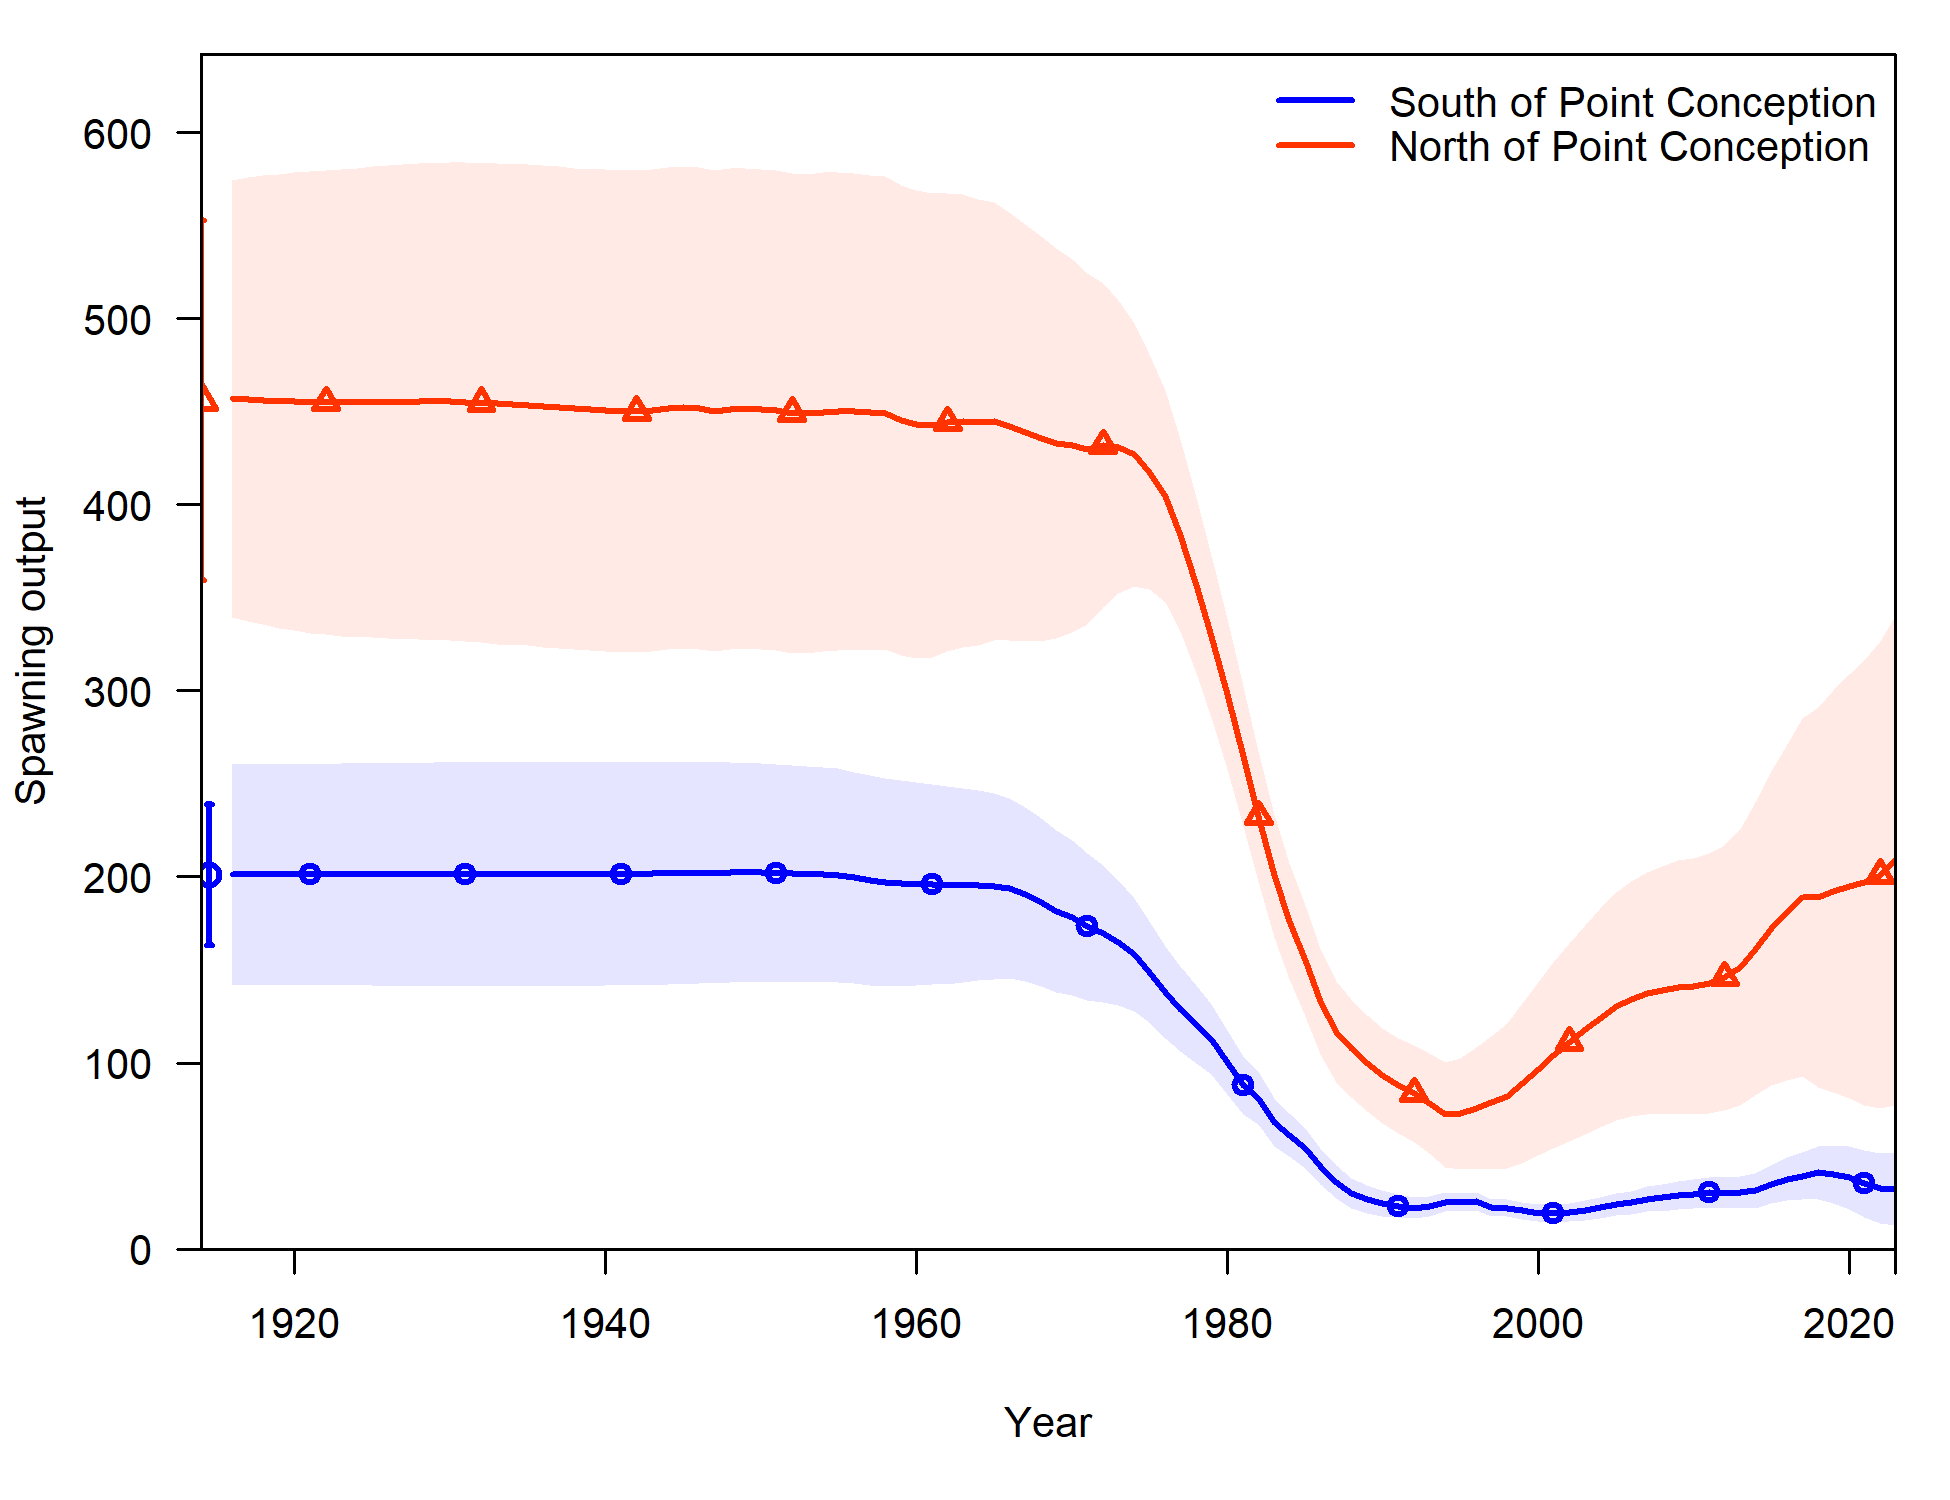
\includegraphics[width=1\textwidth,height=1\textheight]{C:/Assessments/2023/copper_rockfish_2023/documents/shared_figures/compare2_spawnbio_uncertainty.png}
\caption{Estimated time series of spawning output (circles and line: median; light broken lines: 95 percent intervals) for the model areas south and north of Point Conception.\label{fig:es-sb}}
\end{figure}

\begin{figure}
\centering
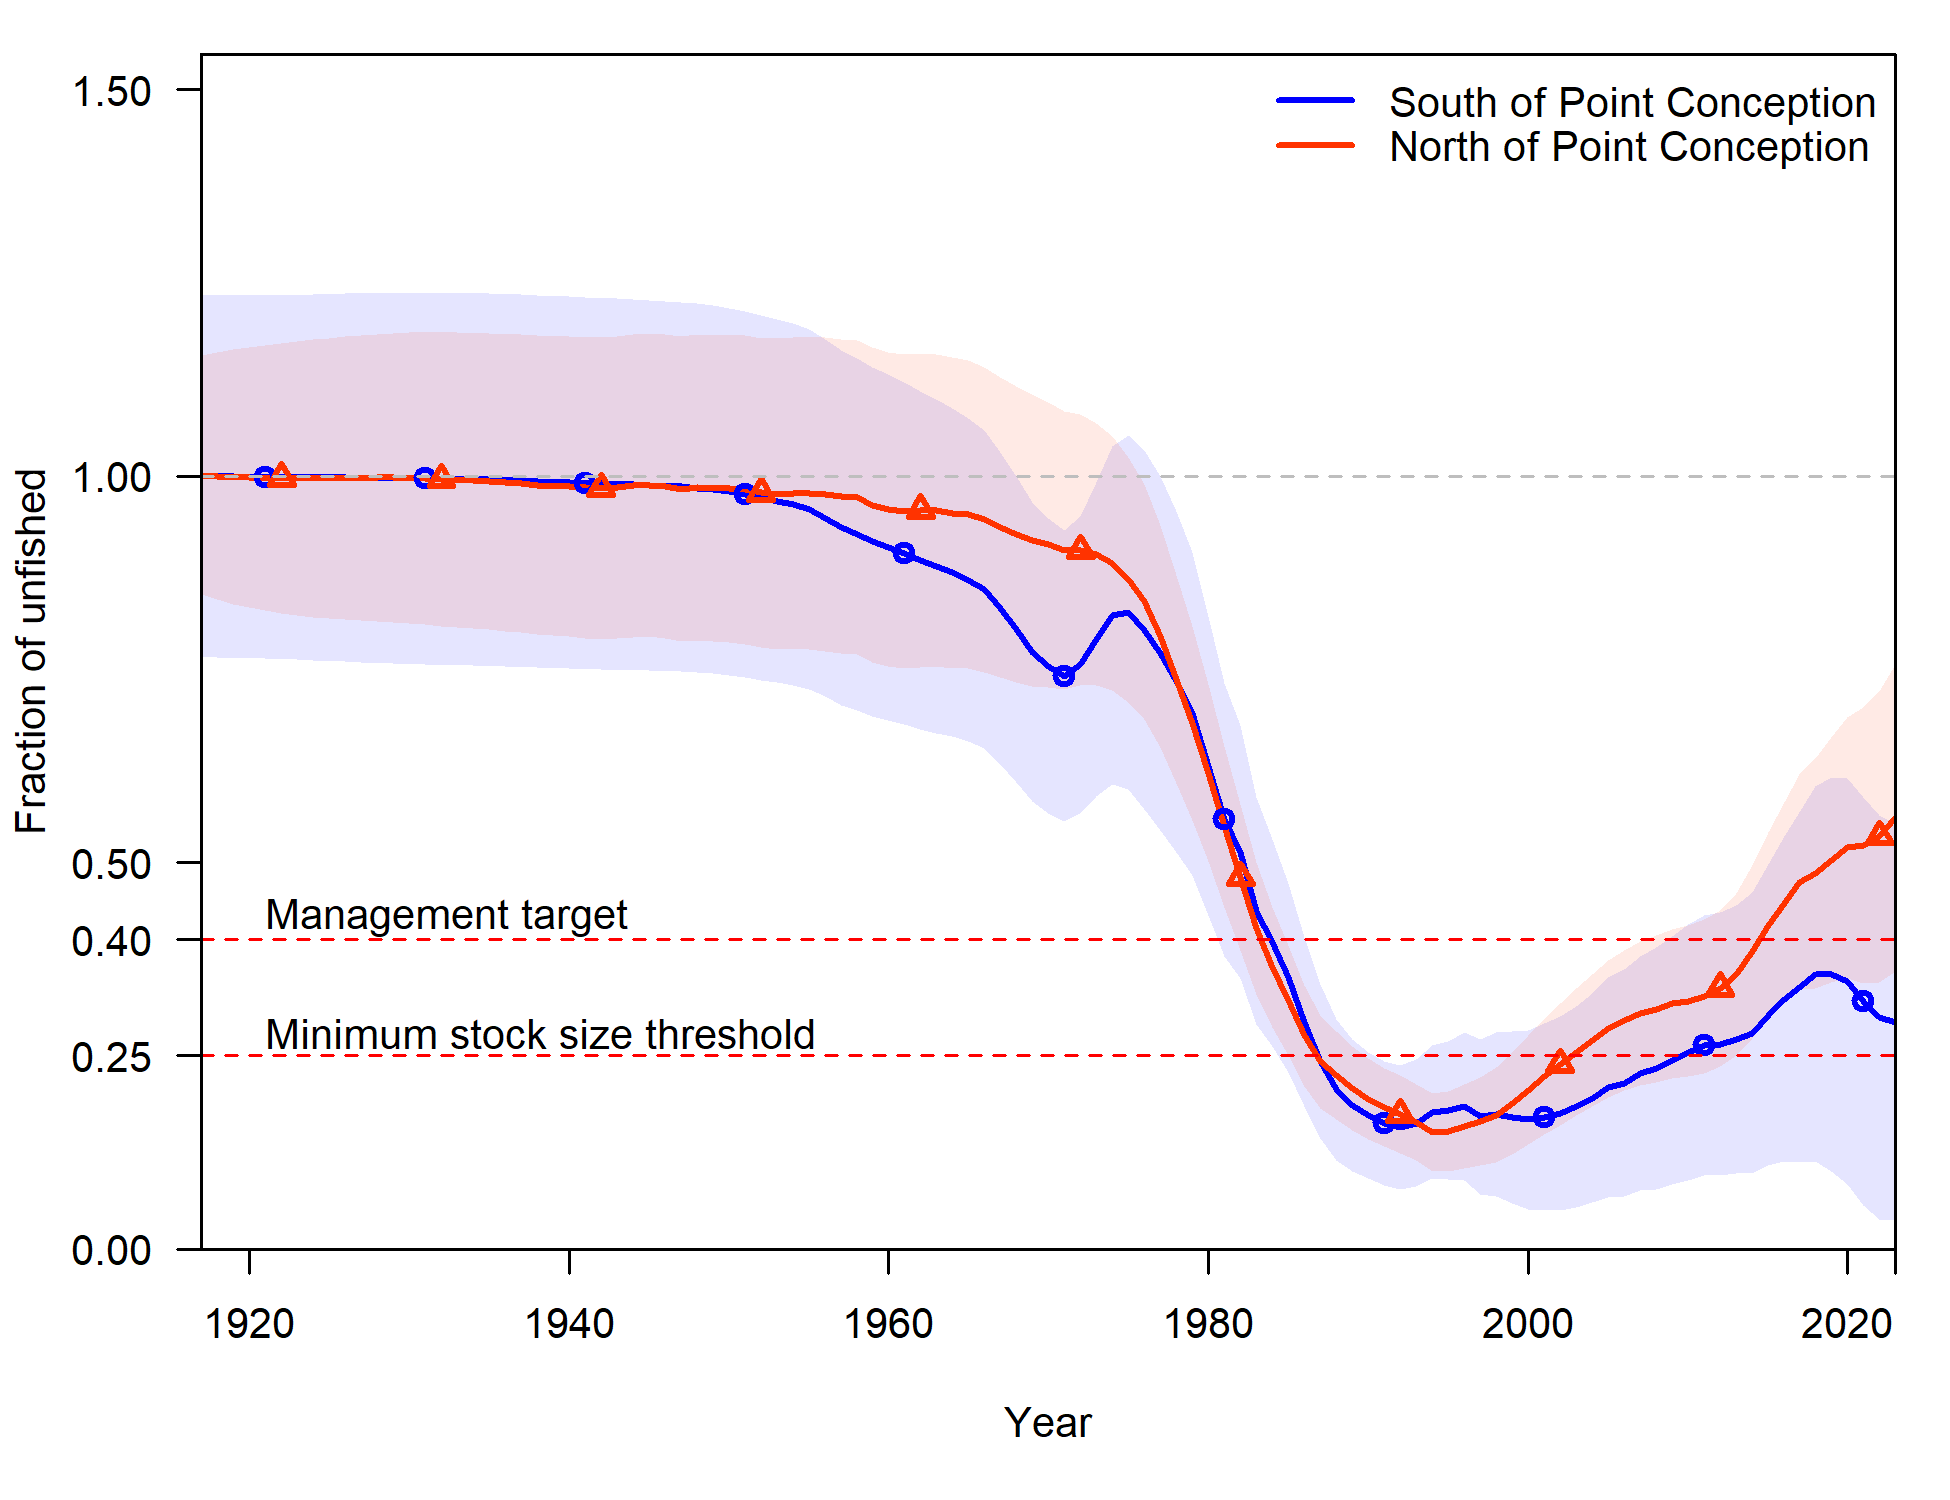
\includegraphics[width=1\textwidth,height=1\textheight]{C:/Assessments/2023/copper_rockfish_2023/documents/shared_figures/compare4_Bratio_uncertainty.png}
\caption{Estimated time series of fraction of unfished spawning output (circles and line: median; light broken lines: 95 percent intervals) for the model areas south and north of Point Conception.\label{fig:es-depl}}
\end{figure}

\clearpage

\hypertarget{recruitment}{%
\subsection*{Recruitment}\label{recruitment}}
\addcontentsline{toc}{subsection}{Recruitment}

Replace text with trends and current levels relative to virgin or historic levels and description of uncertainty. Include Table for last 10 years. Include Figure with long-term estimates.

\begingroup\fontsize{10}{12}\selectfont
\begingroup\fontsize{10}{12}\selectfont

\begin{longtable}[t]{r>{\centering\arraybackslash}p{1.57cm}>{\centering\arraybackslash}p{1.57cm}>{\centering\arraybackslash}p{1.57cm}>{\centering\arraybackslash}p{1.57cm}>{\centering\arraybackslash}p{1.57cm}>{\centering\arraybackslash}p{1.57cm}}
\caption{\label{tab:south-recrES}Estimated recent trend in recruitment and recruitment deviations and the 95 percent intervals for the sub-area model south of Point Conception.}\\
\toprule
Year & Recruitment & Lower Interval & Upper Interval & Recruitment Deviations & Lower Interval & Upper Interval\\
\midrule
\endfirsthead
\caption[]{Estimated recent trend in recruitment and recruitment deviations and the 95 percent intervals for the sub-area model south of Point Conception. \textit{(continued)}}\\
\toprule
Year & Recruitment & Lower Interval & Upper Interval & Recruitment Deviations & Lower Interval & Upper Interval\\
\midrule
\endhead

\endfoot
\bottomrule
\endlastfoot
2013 & 613.62 & 381.00 & 988.26 & 1.18 & 0.94 & 1.41\\
2014 & 168.22 & 86.76 & 326.18 & -0.13 & -0.64 & 0.39\\
2015 & 81.26 & 39.81 & 165.88 & -0.88 & -1.45 & -0.30\\
2016 & 114.55 & 59.49 & 220.57 & -0.55 & -1.00 & -0.09\\
2017 & 91.14 & 44.28 & 187.61 & -0.79 & -1.33 & -0.25\\
2018 & 91.39 & 42.11 & 198.33 & -0.80 & -1.40 & -0.19\\
2019 & 119.56 & 51.10 & 279.76 & -0.53 & -1.24 & 0.18\\
2020 & 119.75 & 43.77 & 327.64 & -0.60 & -1.54 & 0.34\\
2021 & 231.44 & 144.36 & 371.04 & 0.00 & 0.00 & 0.00\\
2022 & 227.42 & 138.88 & 372.42 & 0.00 & 0.00 & 0.00\\
2023 & 226.18 & 137.68 & 371.57 & 0.00 & 0.00 & 0.00\\*
\end{longtable}
\endgroup{}
\endgroup{}


\begingroup\fontsize{10}{12}\selectfont
\begingroup\fontsize{10}{12}\selectfont

\begin{longtable}[t]{r>{\centering\arraybackslash}p{1.57cm}>{\centering\arraybackslash}p{1.57cm}>{\centering\arraybackslash}p{1.57cm}>{\centering\arraybackslash}p{1.57cm}>{\centering\arraybackslash}p{1.57cm}>{\centering\arraybackslash}p{1.57cm}}
\caption{\label{tab:north-recrES}Estimated recent trend in recruitment and recruitment deviations and the 95 percent intervals for the sub-area model north of Point Conception.}\\
\toprule
Year & Recruitment & Lower Interval & Upper Interval & Recruitment Deviations & Lower Interval & Upper Interval\\
\midrule
\endfirsthead
\caption[]{Estimated recent trend in recruitment and recruitment deviations and the 95 percent intervals for the sub-area model north of Point Conception. \textit{(continued)}}\\
\toprule
Year & Recruitment & Lower Interval & Upper Interval & Recruitment Deviations & Lower Interval & Upper Interval\\
\midrule
\endhead

\endfoot
\bottomrule
\endlastfoot
2013 & 556.60 & 282.67 & 1095.99 & 0.23 & -0.38 & 0.84\\
2014 & 466.50 & 233.22 & 933.12 & 0.04 & -0.59 & 0.67\\
2015 & 590.78 & 316.19 & 1103.84 & 0.26 & -0.27 & 0.79\\
2016 & 285.96 & 134.46 & 608.15 & -0.47 & -1.18 & 0.24\\
2017 & 869.76 & 474.53 & 1594.18 & 0.63 & 0.13 & 1.12\\
2018 & 618.32 & 318.82 & 1199.18 & 0.25 & -0.34 & 0.84\\
2019 & 345.34 & 159.74 & 746.57 & -0.37 & -1.11 & 0.37\\
2020 & 502.19 & 394.01 & 640.08 & 0.00 & 0.00 & 0.00\\
2021 & 503.74 & 394.44 & 643.32 & 0.00 & 0.00 & 0.00\\
2022 & 505.86 & 395.70 & 646.68 & 0.00 & 0.00 & 0.00\\
2023 & 509.39 & 398.85 & 650.56 & 0.00 & 0.00 & 0.00\\*
\end{longtable}
\endgroup{}
\endgroup{}


\begin{figure}
\centering
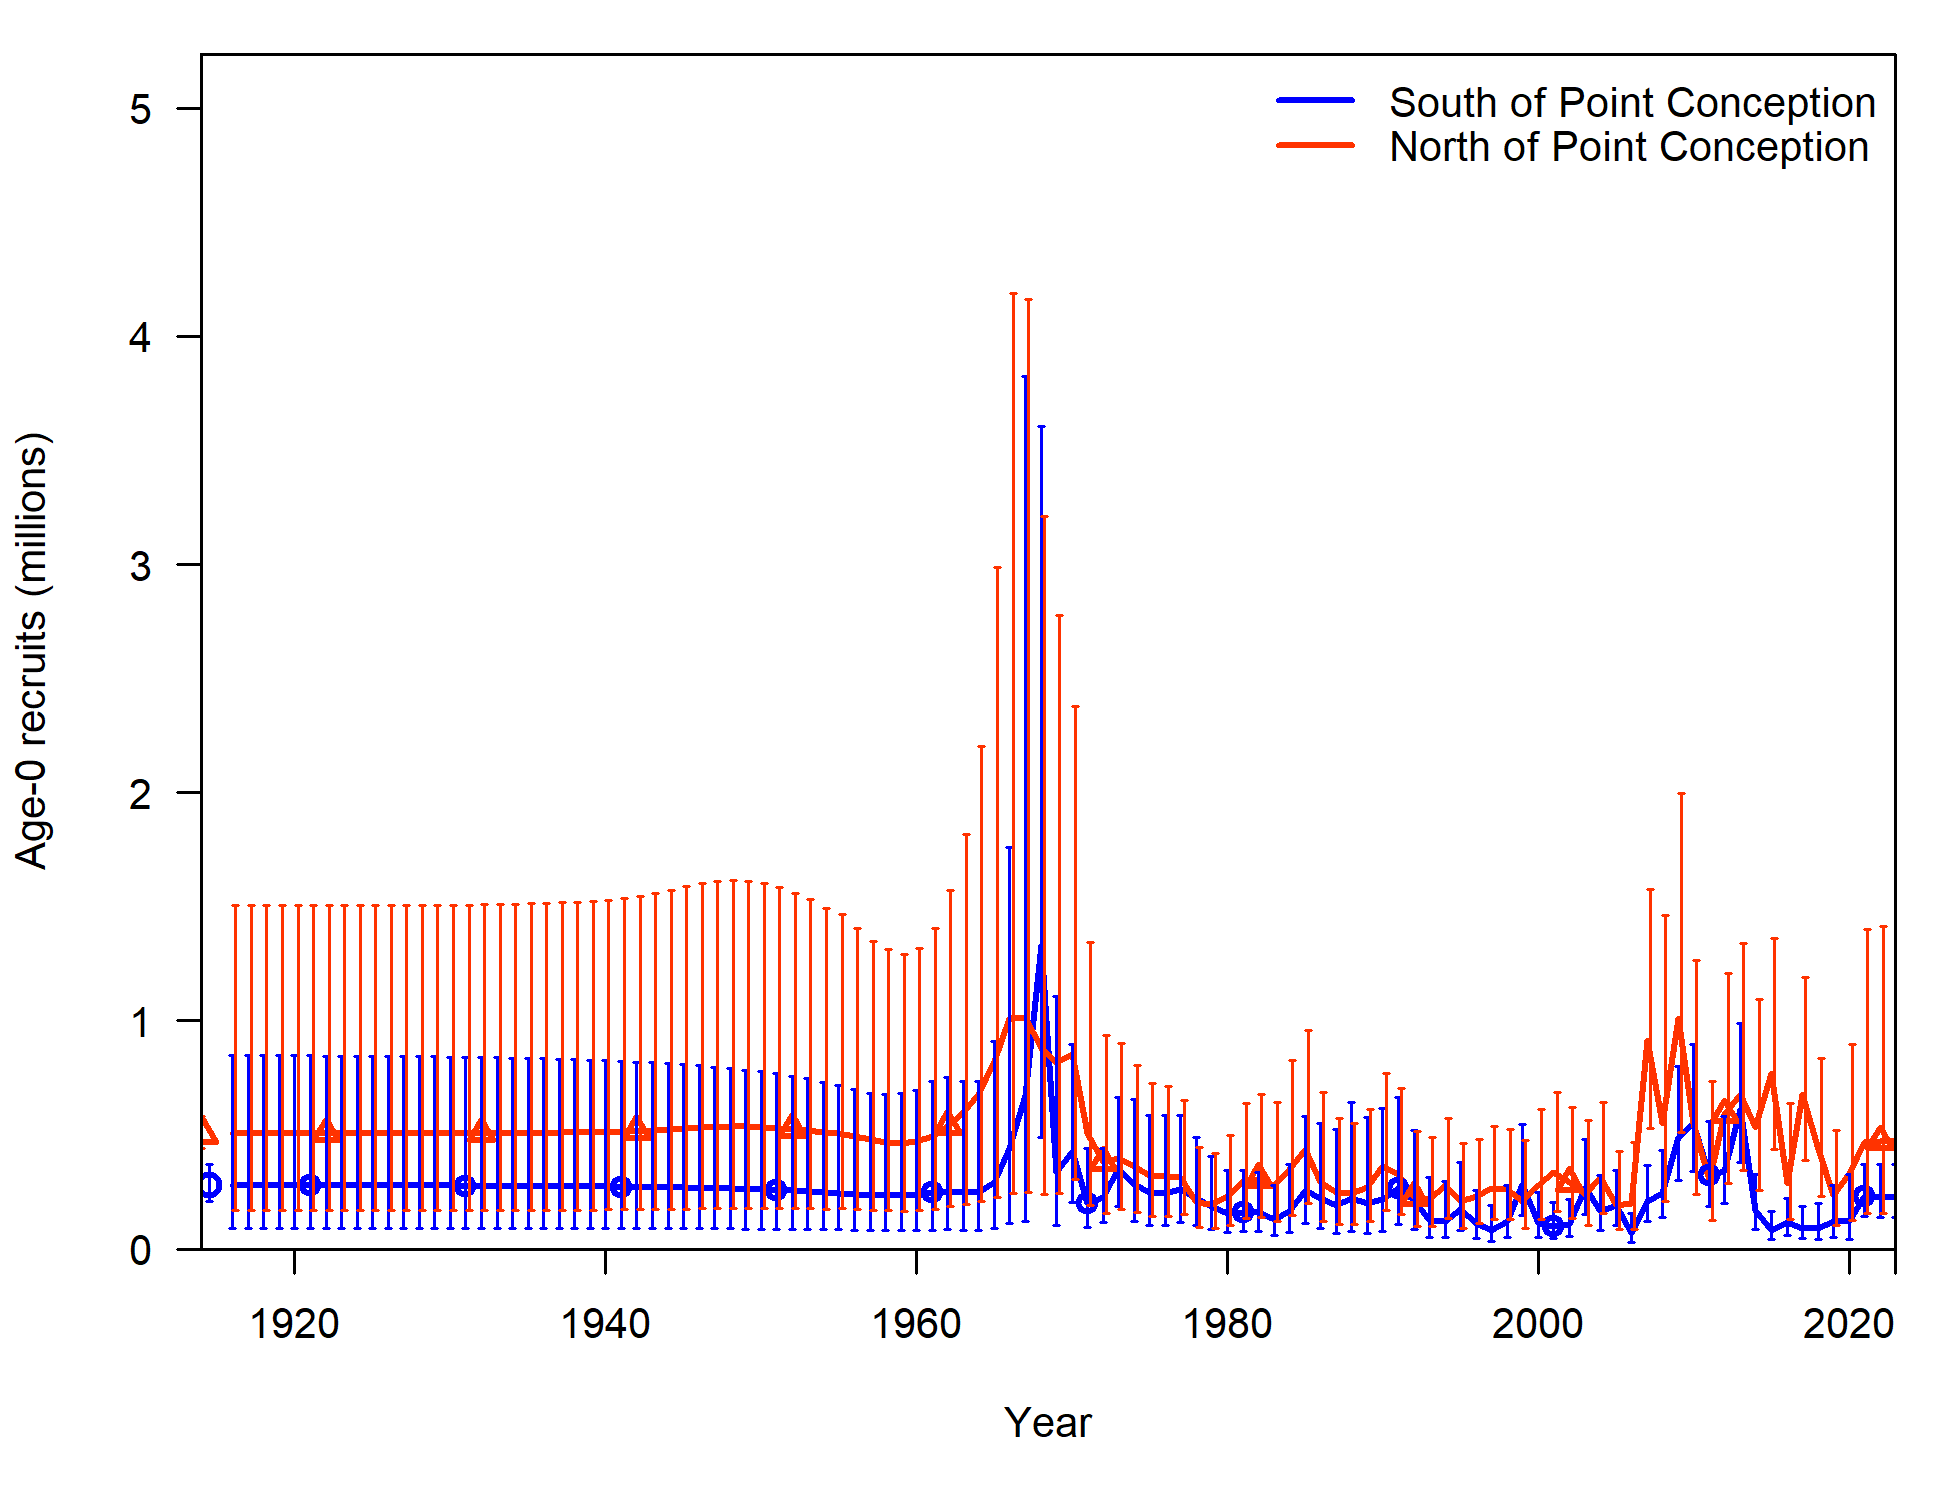
\includegraphics[width=1\textwidth,height=1\textheight]{C:/Assessments/2023/copper_rockfish_2023/documents/shared_figures/compare10_recruits_uncertainty.png}
\caption{Estimated time series of age-0 recruits (1000s) for the model areas south and north of Point Conception with 95 percent intervals.\label{fig:es-recruits}}
\end{figure}

\begin{figure}
\centering
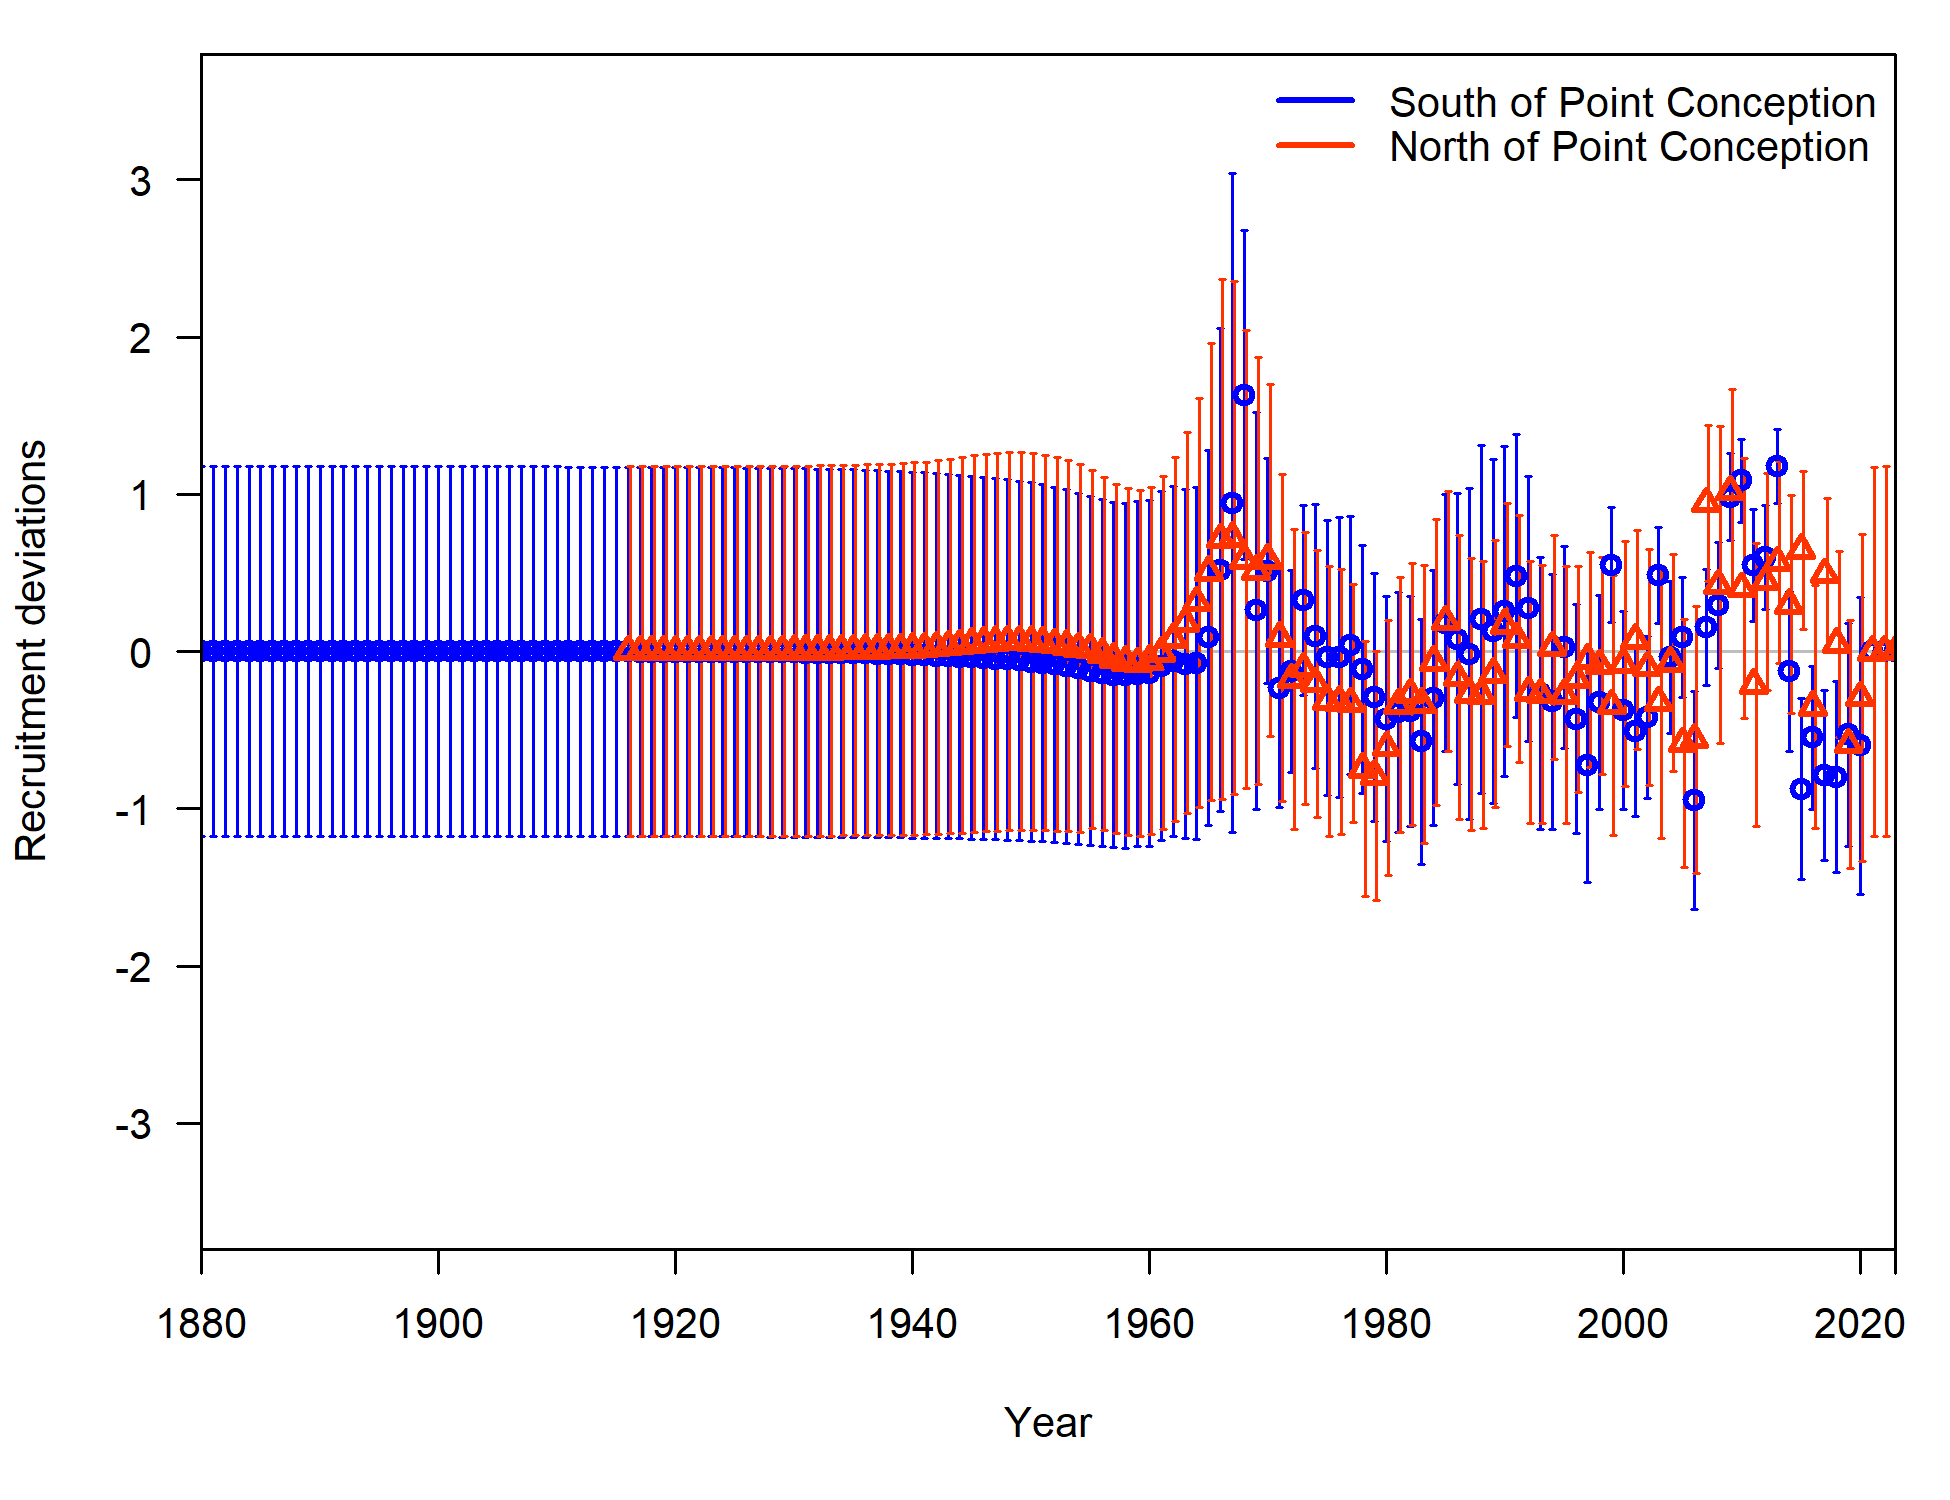
\includegraphics[width=1\textwidth,height=1\textheight]{C:/Assessments/2023/copper_rockfish_2023/documents/shared_figures/compare12_recdevs_uncertainty.png}
\caption{Estimated time series of recruitment deviations for the model areas south and north of Point Conception.\label{fig:es-rec-devs}}
\end{figure}

\clearpage

\hypertarget{exploitation-status}{%
\subsection*{Exploitation status}\label{exploitation-status}}
\addcontentsline{toc}{subsection}{Exploitation status}

Replace text with total catch divided by exploitable biomass or SPR harvest rate. Include Table for last 10 years. Include Figure with trend in f relative to target vs.~trend in biomass relative to the target.

\begingroup\fontsize{10}{12}\selectfont
\begingroup\fontsize{10}{12}\selectfont

\begin{longtable}[t]{r>{\centering\arraybackslash}p{1.57cm}>{\centering\arraybackslash}p{1.57cm}>{\centering\arraybackslash}p{1.57cm}>{\centering\arraybackslash}p{1.57cm}>{\centering\arraybackslash}p{1.57cm}>{\centering\arraybackslash}p{1.57cm}}
\caption{\label{tab:south-exploitES}Estimated recent trend in the 1-SPR where SPR is the spawning potential ratio the exploitation rate, and the 95 percent intervals for the sub-area model south of Point Conception.}\\
\toprule
Year & 1-SPR & Lower Interval & Upper Interval & Exploitation Rate & Lower Interval & Upper Interval\\
\midrule
\endfirsthead
\caption[]{Estimated recent trend in the 1-SPR where SPR is the spawning potential ratio the exploitation rate, and the 95 percent intervals for the sub-area model south of Point Conception. \textit{(continued)}}\\
\toprule
Year & 1-SPR & Lower Interval & Upper Interval & Exploitation Rate & Lower Interval & Upper Interval\\
\midrule
\endhead

\endfoot
\bottomrule
\endlastfoot
2013 & 0.71 & 0.52 & 0.90 & 0.11 & 0.05 & 0.17\\
2014 & 0.59 & 0.39 & 0.79 & 0.08 & 0.04 & 0.13\\
2015 & 0.66 & 0.46 & 0.86 & 0.10 & 0.05 & 0.16\\
2016 & 0.71 & 0.51 & 0.90 & 0.12 & 0.05 & 0.18\\
2017 & 0.67 & 0.46 & 0.88 & 0.10 & 0.04 & 0.16\\
2018 & 0.75 & 0.55 & 0.95 & 0.12 & 0.05 & 0.20\\
2019 & 0.72 & 0.50 & 0.94 & 0.11 & 0.03 & 0.18\\
2020 & 0.80 & 0.59 & 1.01 & 0.12 & 0.03 & 0.21\\
2021 & 0.72 & 0.47 & 0.98 & 0.09 & 0.02 & 0.17\\
2022 & 0.40 & 0.15 & 0.64 & 0.03 & 0.01 & 0.06\\*
\end{longtable}
\endgroup{}
\endgroup{}


\begingroup\fontsize{10}{12}\selectfont
\begingroup\fontsize{10}{12}\selectfont

\begin{longtable}[t]{r>{\centering\arraybackslash}p{1.57cm}>{\centering\arraybackslash}p{1.57cm}>{\centering\arraybackslash}p{1.57cm}>{\centering\arraybackslash}p{1.57cm}>{\centering\arraybackslash}p{1.57cm}>{\centering\arraybackslash}p{1.57cm}}
\caption{\label{tab:north-exploitES}Estimated recent trend in the 1-SPR where SPR is the spawning potential ratio the exploitation rate, and the 95 percent intervals for the sub-area model north of Point Conception.}\\
\toprule
Year & 1-SPR & Lower Interval & Upper Interval & Exploitation Rate & Lower Interval & Upper Interval\\
\midrule
\endfirsthead
\caption[]{Estimated recent trend in the 1-SPR where SPR is the spawning potential ratio the exploitation rate, and the 95 percent intervals for the sub-area model north of Point Conception. \textit{(continued)}}\\
\toprule
Year & 1-SPR & Lower Interval & Upper Interval & Exploitation Rate & Lower Interval & Upper Interval\\
\midrule
\endhead

\endfoot
\bottomrule
\endlastfoot
2013 & 0.16 & 0.10 & 0.22 & 0.01 & 0.01 & 0.02\\
2014 & 0.20 & 0.13 & 0.27 & 0.02 & 0.01 & 0.02\\
2015 & 0.31 & 0.21 & 0.41 & 0.03 & 0.02 & 0.04\\
2016 & 0.31 & 0.20 & 0.41 & 0.03 & 0.02 & 0.04\\
2017 & 0.50 & 0.37 & 0.63 & 0.05 & 0.03 & 0.08\\
2018 & 0.41 & 0.28 & 0.53 & 0.04 & 0.02 & 0.06\\
2019 & 0.40 & 0.27 & 0.53 & 0.04 & 0.02 & 0.06\\
2020 & 0.53 & 0.38 & 0.67 & 0.06 & 0.03 & 0.08\\
2021 & 0.41 & 0.27 & 0.55 & 0.04 & 0.02 & 0.06\\
2022 & 0.21 & 0.12 & 0.30 & 0.02 & 0.01 & 0.03\\*
\end{longtable}
\endgroup{}
\endgroup{}


\begin{figure}
\centering
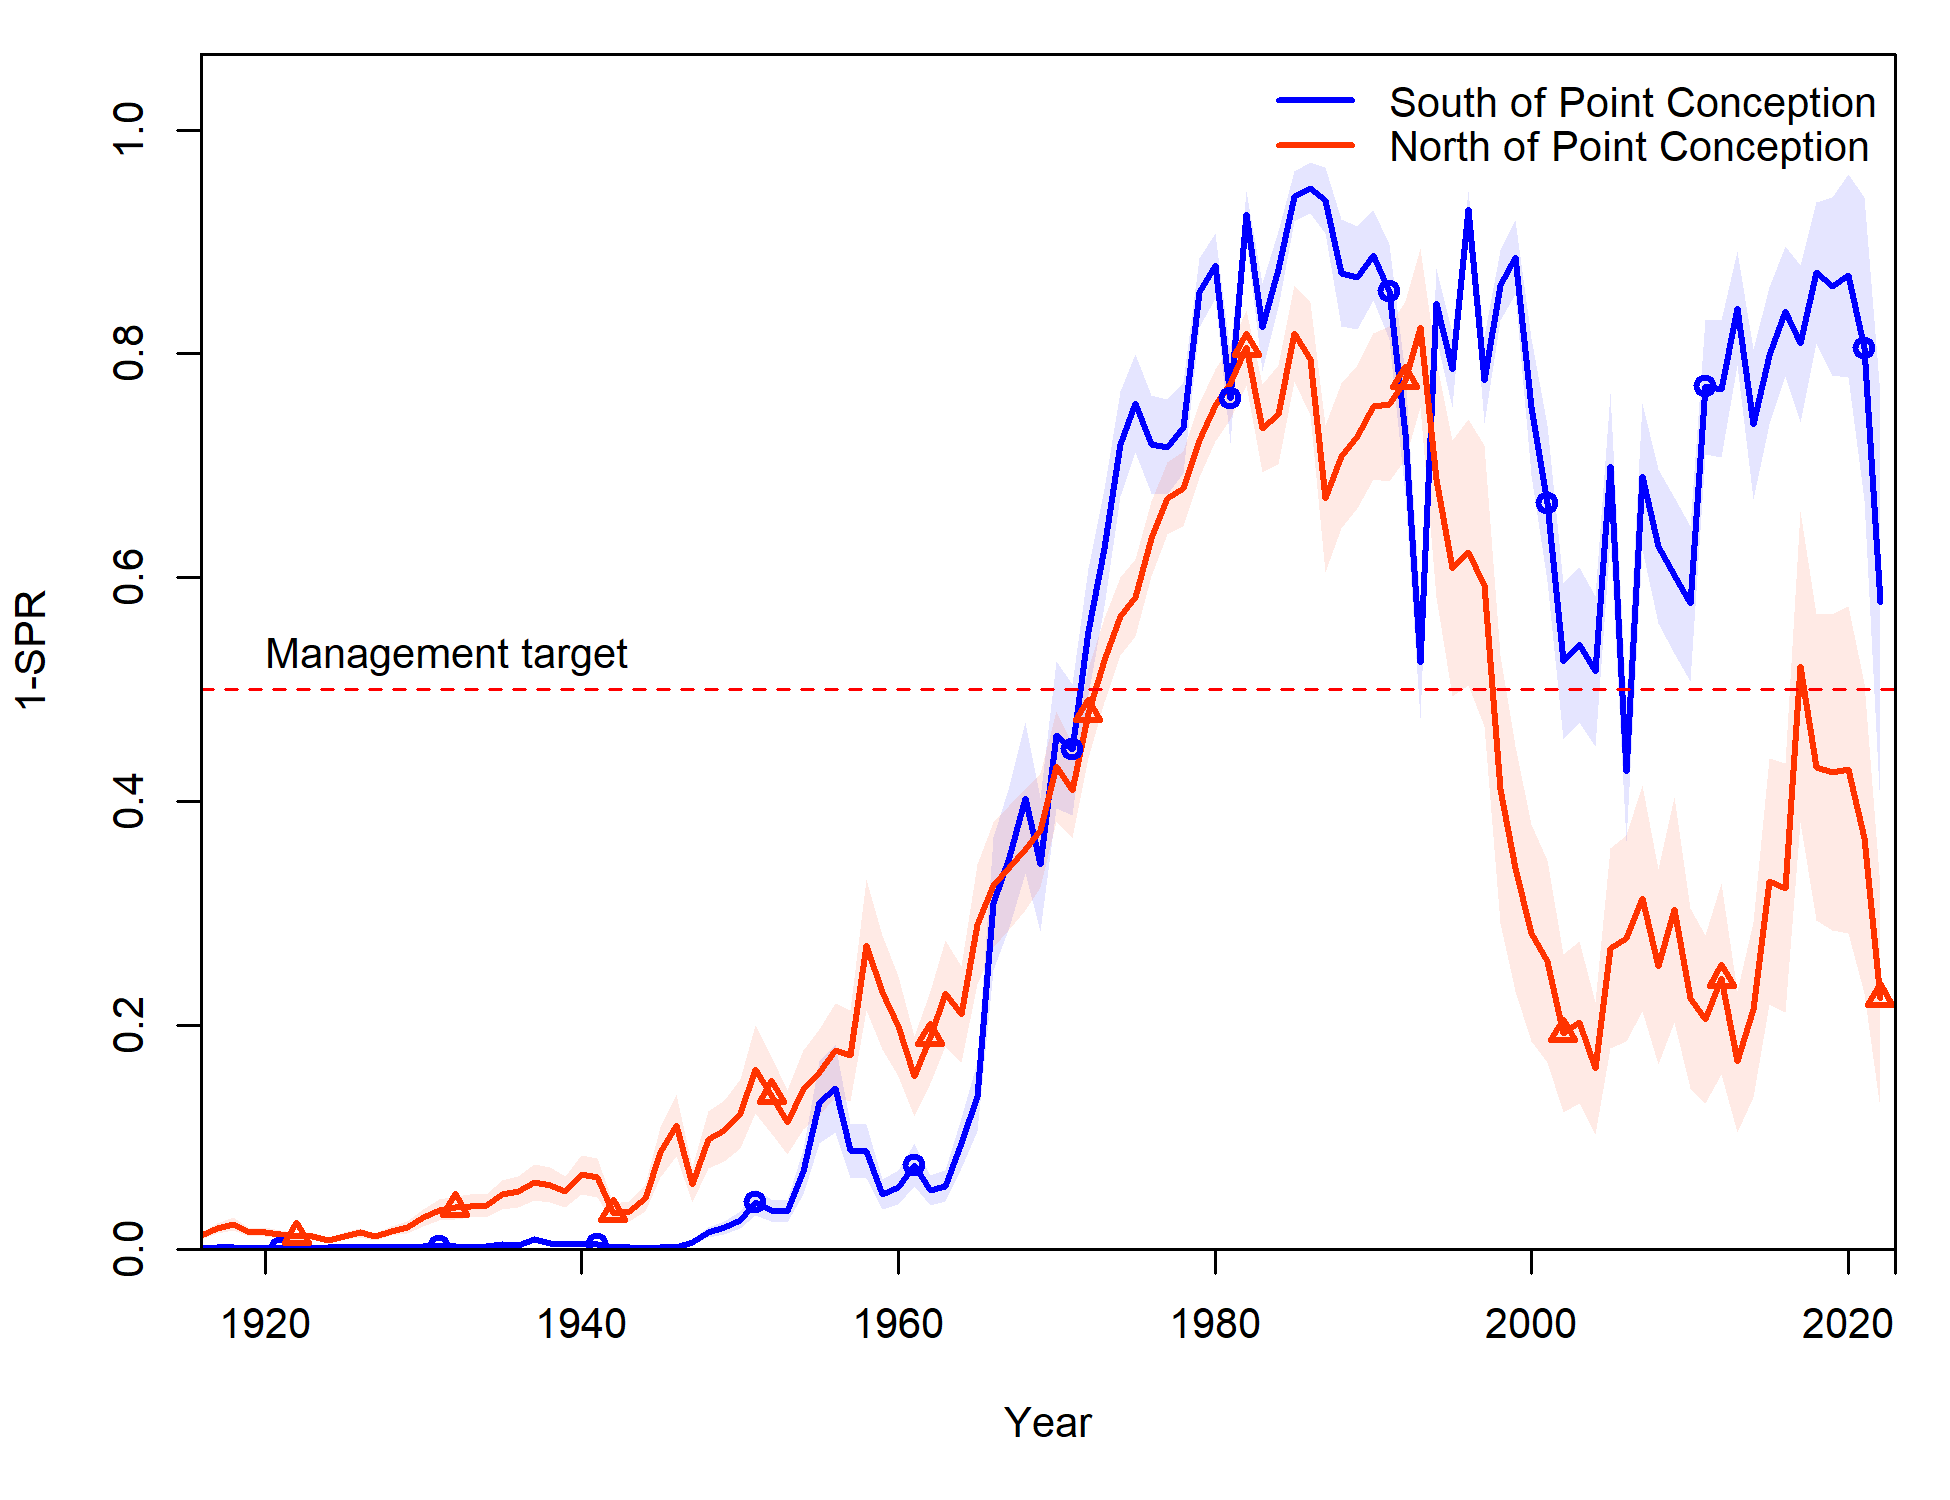
\includegraphics[width=1\textwidth,height=1\textheight]{C:/Assessments/2023/copper_rockfish_2023/documents/shared_figures/compare6_SPRratio_uncertainty.png}
\caption{Estimated 1 - relative spawning ratio (SPR) by year for the model areas south and north of Point Conception. The management target is plotted as a red horizontal line and values above this reflect harvest in excess of the proxy harvest rate.\label{fig:es-1-spr}}
\end{figure}

\hypertarget{ecosystem-considerations}{%
\subsection*{Ecosystem considerations}\label{ecosystem-considerations}}
\addcontentsline{toc}{subsection}{Ecosystem considerations}

shared text

\hypertarget{reference-points}\), i.e., the \(B_{MSY}\) proxy and the equilibrium stock size that results from fishing at the default harvest rate, i.e., the \(F_{MSY}\) proxy. Include Table of estimated reference points for ssb, SPR, exploitation rate, and yield based on SSB proxy for MSY, SPR proxy for MSY, and estimated MSY values.

\begingroup\fontsize{10}{12}\selectfont
\begingroup\fontsize{10}{12}\selectfont

\begin{longtable}[t]{r>{\centering\arraybackslash}p{2cm}>{\centering\arraybackslash}p{2cm}>{\centering\arraybackslash}p{2cm}}
\caption{\label{tab:south-referenceES}Summary of reference points and management quantities, including estimates of the 95 percent intervals for the sub-area model south of Point Conception.}\\
\toprule
 & Estimate & Lower Interval & Upper Interval\\
\midrule
\endfirsthead
\caption[]{Summary of reference points and management quantities, including estimates of the 95 percent intervals for the sub-area model south of Point Conception. \textit{(continued)}}\\
\toprule
 & Estimate & Lower Interval & Upper Interval\\
\midrule
\endhead

\endfoot
\bottomrule
\endlastfoot
Unfished Spawning Output & 201.06 & 163.43 & 238.70\\
Unfished Age 3+ Biomass (mt) & 1999.51 & 1624.90 & 2374.12\\
Unfished Recruitment (R0) & 241.18 & 196.04 & 286.32\\
Spawning Output (2023) & 32.06 & 12.70 & 51.42\\
Fraction Unfished (2023) & 0.16 & 0.06 & 0.25\\
Reference Points Based SB40\% &  &  & \\
Proxy Spawning Output SB40\% & 80.43 & 65.37 & 95.48\\
SPR Resulting in SB40\% & 0.46 & 0.46 & 0.46\\
Exploitation Rate Resulting in SB40\% & 0.06 & 0.05 & 0.06\\
Yield with SPR Based On SB40\% (mt) & 49.99 & 40.74 & 59.25\\
Reference Points Based on SPR Proxy for MSY &  &  & \\
Proxy Spawning Output (SPR50) & 89.71 & 72.92 & 106.50\\
SPR50 & 0.50 & - & -\\
Exploitation Rate Corresponding to SPR50 & 0.05 & 0.05 & 0.05\\
Yield with SPR50 at SB SPR (mt) & 47.78 & 38.93 & 56.62\\
Reference Points Based on Estimated MSY Values &  &  & \\
Spawning Output at MSY (SB MSY) & 55.51 & 45.15 & 65.87\\
SPR MSY & 0.35 & 0.34 & 0.35\\
Exploitation Rate Corresponding to SPR MSY & 0.08 & 0.08 & 0.08\\
MSY (mt) & 52.94 & 43.14 & 62.74\\*
\end{longtable}
\endgroup{}
\endgroup{}


\begingroup\fontsize{10}{12}\selectfont
\begingroup\fontsize{10}{12}\selectfont

\begin{longtable}[t]{r>{\centering\arraybackslash}p{2cm}>{\centering\arraybackslash}p{2cm}>{\centering\arraybackslash}p{2cm}}
\caption{\label{tab:north-referenceES}Summary of reference points and management quantities, including estimates of the 95 percent intervals for the sub-area model north of Point Conception.}\\
\toprule
 & Estimate & Lower Interval & Upper Interval\\
\midrule
\endfirsthead
\caption[]{Summary of reference points and management quantities, including estimates of the 95 percent intervals for the sub-area model north of Point Conception. \textit{(continued)}}\\
\toprule
 & Estimate & Lower Interval & Upper Interval\\
\midrule
\endhead

\endfoot
\bottomrule
\endlastfoot
Unfished Spawning Output & 486.15 & 387.43 & 584.87\\
Unfished Age 3+ Biomass (mt) & 4719.91 & 3777.92 & 5661.90\\
Unfished Recruitment (R0) & 567.77 & 452.48 & 683.06\\
Spawning Output (2023) & 262.10 & 124.28 & 399.92\\
Fraction Unfished (2023) & 0.54 & 0.32 & 0.76\\
Reference Points Based SB40\% &  &  & \\
Proxy Spawning Output SB40\% & 194.46 & 154.97 & 233.95\\
SPR Resulting in SB40\% & 0.46 & 0.46 & 0.46\\
Exploitation Rate Resulting in SB40\% & 0.06 & 0.06 & 0.06\\
Yield with SPR Based On SB40\% (mt) & 129.86 & 104.05 & 155.67\\
Reference Points Based on SPR Proxy for MSY &  &  & \\
Proxy Spawning Output (SPR50) & 216.90 & 172.85 & 260.94\\
SPR50 & 0.50 &  & \\
Exploitation Rate Corresponding to SPR50 & 0.05 & 0.05 & 0.05\\
Yield with SPR50 at SB SPR (mt) & 124.05 & 99.39 & 148.71\\
Reference Points Based on Estimated MSY Values &  &  & \\
Spawning Output at MSY (SB MSY) & 134.17 & 106.84 & 161.51\\
SPR MSY & 0.35 & 0.34 & 0.35\\
Exploitation Rate Corresponding to SPR MSY & 0.09 & 0.08 & 0.09\\
MSY (mt) & 137.59 & 110.25 & 164.92\\*
\end{longtable}
\endgroup{}
\endgroup{}


\begin{figure}
\centering
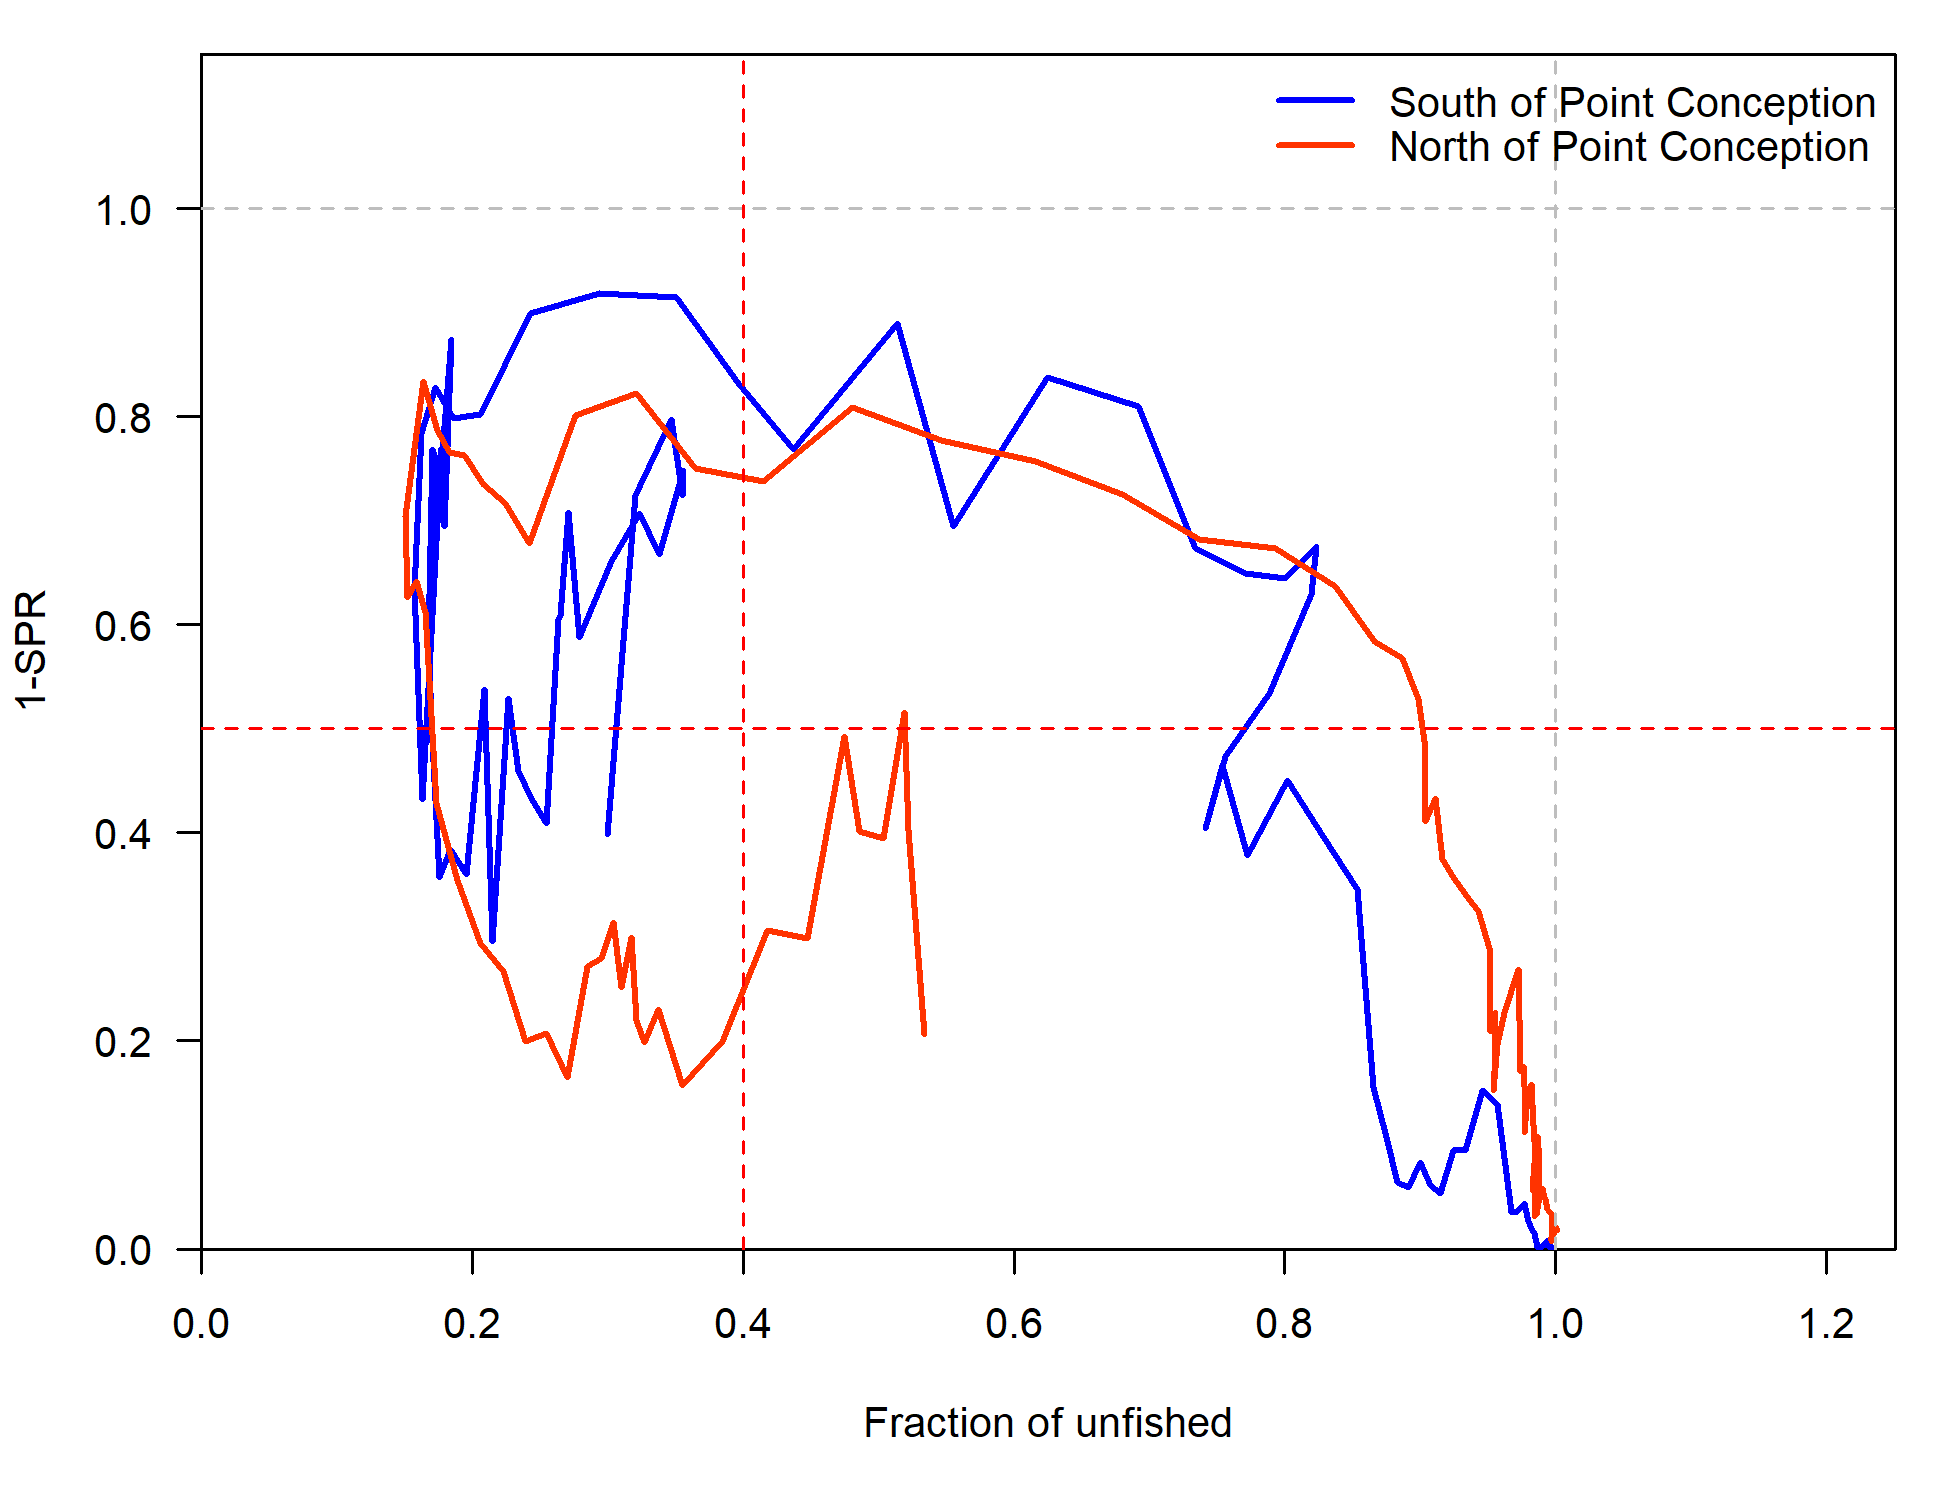
\includegraphics[width=1\textwidth,height=1\textheight]{C:/Assessments/2023/copper_rockfish_2023/documents/shared_figures/compare15_phase_plot.png}
\caption{Phase plot of estimated 1-SPR versus fraction unfished for the model areas south and north of Point Conception.\label{fig:es-phase}}
\end{figure}

\begin{figure}
\centering
\includegraphics[width=1\textwidth,height=1\textheight]{N:/Assessments/CurrentAssessments/copper_rockfish_2023/models/sca/14.0_base/plots/yield2_yield_curve_with_refpoints.png}
\caption{Equilibrium yield curve for the base case model for model south of Point Conception. Values are based on the 2022 fishery selectivities and with steepness fixed at 0.72.\label{fig:south-es-yield}}
\end{figure}

\begin{figure}
\centering
\includegraphics[width=1\textwidth,height=1\textheight]{N:/Assessments/CurrentAssessments/copper_rockfish_2023/models/nca/9.8_selex_fix/plots/yield2_yield_curve_with_refpoints.png}
\caption{Equilibrium yield curve for the base case model for model north of Point Conception. Values are based on the 2022 fishery selectivities and with steepness fixed at 0.72.\label{fig:north-es-yield}}
\end{figure}

\hypertarget{management-performance}{%
\subsection*{Management performance}\label{management-performance}}
\addcontentsline{toc}{subsection}{Management performance}

Include Table of most recent 10 years of catches in comparison with OFL, ABC, HG, and OY/ACL values, overfishing levels, actual catch and discard. Include OFL (encountered), OFL (retained), and OFL (dead) if different due to discard and discard mortality.

\begingroup\fontsize{10}{12}\selectfont
\begingroup\fontsize{10}{12}\selectfont

\begin{longtable}[t]{c>{\centering\arraybackslash}p{2cm}>{\centering\arraybackslash}p{2cm}>{\centering\arraybackslash}p{2cm}}
\caption{\label{tab:es-ca-management}The portion of the Overfishing Limit (OFL) and Annual Catch Limit (ACL) and estimated catch in California waters.}\\
\toprule
Year & OFL (mt) & ACL (mt) & Catch (mt)\\
\midrule
\endfirsthead
\caption[]{\label{tab:es-ca-management}The portion of the Overfishing Limit (OFL) and Annual Catch Limit (ACL) and estimated catch in California waters. \textit{(continued)}}\\
\toprule
Year & OFL (mt) & ACL (mt) & Catch (mt)\\
\midrule
\endhead

\endfoot
\bottomrule
\endlastfoot
2012 & 163.15 & 136.17 & 85.95\\
2013 & 148.00 & 123.42 & 105.18\\
2014 & 148.00 & 123.42 & 98.65\\
2015 & 303.75 & 277.32 & 147.64\\
2016 & 286.88 & 261.95 & 165.27\\
2017 & 313.70 & 286.38 & 225.48\\
2018 & 319.60 & 291.85 & 203.69\\
2019 & 325.08 & 296.83 & 182.59\\
2020 & 330.35 & 301.60 & 242.73\\
2021 & 249.85 & 206.43 & 164.20\\
2022 & 249.48 & 204.02 & 66.67\\*
\end{longtable}
\endgroup{}
\endgroup{}

\hypertarget{unresolved-problems-and-major-uncertainties}{%
\subsection*{Unresolved problems and major uncertainties}\label{unresolved-problems-and-major-uncertainties}}
\addcontentsline{toc}{subsection}{Unresolved problems and major uncertainties}

shared text

\hypertarget{decision-table-and-projections}{%
\subsection*{Decision table and projections}\label{decision-table-and-projections}}
\addcontentsline{toc}{subsection}{Decision table and projections}

Replace text with projected yields (OFL, ABC, and ACL), spawning biomass, and stock depletion levels for each year. OFL calculations should be based on the assumption that future catches equal ABCs and not OFLs.

\begingroup\fontsize{10}{12}\selectfont

\begin{landscape}\begingroup\fontsize{10}{12}\selectfont

\begin{longtable}[t]{c>{\centering\arraybackslash}p{1.38cm}>{\centering\arraybackslash}p{1.38cm}>{\centering\arraybackslash}p{1.38cm}>{\centering\arraybackslash}p{1.38cm}>{\centering\arraybackslash}p{1.38cm}>{\centering\arraybackslash}p{1.38cm}>{\centering\arraybackslash}p{1.38cm}}
\caption{\label{tab:es-ca-proj}The estimated spawning output in number of million eggs across California and fraction unfished by year.}\\
\toprule
Year & Adopted OFL (mt) & Adopted ABC (mt) & Assumed Catch (mt) & OFL (mt) & ABC (mt) & Spawning Biomass & Fraction Unfished\\
\midrule
\endfirsthead
\caption[]{\label{tab:es-ca-proj}The estimated spawning output in number of million eggs across California and fraction unfished by year. \textit{(continued)}}\\
\toprule
Year & Adopted OFL (mt) & Adopted ABC (mt) & Assumed Catch (mt) & OFL (mt) & ABC (mt) & Spawning Biomass & Fraction Unfished\\
\midrule
\endhead

\endfoot
\bottomrule
\endlastfoot
2023 & 116.4 & 91.53 & 91.5 & - & - & 299.85 & 0.435\\
2024 & 121.32 & 94.69 & 94.7 & - & - & 300.68 & 0.436\\
2025 & - & - & - & 169.81 & 150.5 & 300.32 & 0.436\\
2026 & - & - & - & 170.46 & 150.08 & 300.93 & 0.436\\
2027 & - & - & - & 171.19 & 150.54 & 301.21 & 0.437\\
2028 & - & - & - & 171.73 & 151.57 & 301.58 & 0.437\\
2029 & - & - & - & 172.01 & 152.73 & 302.10 & 0.438\\
2030 & - & - & - & 172.1 & 153.81 & 302.69 & 0.439\\
2031 & - & - & - & 172.14 & 154.73 & 303.28 & 0.440\\
2032 & - & - & - & 172.22 & 155.53 & 303.84 & 0.441\\
2033 & - & - & - & 172.38 & 156.29 & 304.41 & 0.442\\
2034 & - & - & - & 172.63 & 157.04 & 305.03 & 0.442\\*
\end{longtable}
\endgroup{}
\end{landscape}
\endgroup{}

\hypertarget{scientific-uncertainty}{%
\subsection*{Scientific uncertainty}\label{scientific-uncertainty}}
\addcontentsline{toc}{subsection}{Scientific uncertainty}

The model estimated uncertainty around the 2023 spawning output was \(\sigma\) = 0.29 and the uncertainty around the OFL was \(\sigma\) = 0.27. This is likely an underestimate of overall uncertainty because of the necessity to fix several population dynamic parameters (e.g., steepness, recruitment variance, female natural mortality) and no explicit incorporation of model structural uncertainty (although see the decision table for alternative states of nature).

\hypertarget{research-and-data-needs}{%
\subsection*{Research and data needs}\label{research-and-data-needs}}
\addcontentsline{toc}{subsection}{Research and data needs}

shared text

\pagebreak
\setlength{\parskip}{5mm plus1mm minus1mm}
\pagenumbering{arabic}
\setcounter{page}{1}
\renewcommand{\thefigure}{\arabic{figure}}
\renewcommand{\thetable}{\arabic{table}}
\setcounter{table}{0}
\setcounter{figure}{0}

\hypertarget{introduction}{%
\section{Introduction}\label{introduction}}

This assessment report describes the sub-area population of copper rockfish (\emph{Sebastes caurinus}) off the California coast south of Point Conception in U.S. waters, using data through 2022. The sub-area population north of Point Conception in California waters was also evaluated and is described in a separate assessment report. The copper rockfish status for the California stock of is determined by the combined estimates of spawning output from both sub-areas and is detailed in the \protect\hyperlink{management}{Management} section. This assessment does not account for populations located in Mexico waters or other areas off the U.S. coast and assumes that these southern and northern populations do not contribute to the population being assessed here.

\hypertarget{basic-information-and-life-history}{%
\subsection{Basic Information and Life History}\label{basic-information-and-life-history}}

Copper rockfish have historically been a part of both commercial and recreational fisheries throughout its range. Copper rockfish are a demersal, relatively nearshore species within the subgenus \emph{Pteropodus.} The copper rockfish's core range is c omparatively large, ranging from northern Baja Mexico to the Gulf of Alaska, with copper rockfish also found in Puget Sound. Copper rockfish range from the subtidal (as juveniles) to depths of 183 m (Love et al. 2002). Copper rockfish are commonly found in waters less than 100 meters in depth inhabiting nearshore kelp forests and complex low-relief rocky habitat (Love 1996). Adult copper rockfish have high site fidelity and do not make long-range movements. An acoustic telemetry study displaced copper rockfish 4km from their capture location to an artificial reef and within 10 days, half of the copper rockfish returned to the original capture location (Reynolds et al. 2010).

Copper rockfish have a clearly defined long white band the posterior two-thirds of the lateral line. Copper rockfish has high variation in coloration throughout its range, taking on coloration from dark brown, olive, orange-red and pink, with patches of yellow and pink (Miller and Lea 1972). In general the copper rockfish towards the northern part of the range are often darker in color than fish encountered in southern California. The distinct change in coloration resulted in copper rockfish described as two separate species, copper rockfish (\emph{S. caurinus}) and whitebelly rockfish (\emph{S. vexillaris}).

The \emph{Sebastes} genus are viviparous with internal fertilization, many exhibit dimorphic growth with females larger at size-at-age than males, and a number of species have reproductive strategies that vary with latitude. There are very few fecundity samples from copper rockfish available from available from California, although copper rockfish are assumed to produce a single brood annually during the winter months.

The pelagic larvae are encountered in the CalCOFI surveys, but neither larval nor young-of-the-year (YOY) can be identified copper rockfish visually (Thompson et al. 2017). The size at birth ranges from 5-6 mm and the larvae remain pelagic until approximately 22-23 mm standard length at which time they recruit to the kelp forest canopy (Anderson 1983).

Juvenile Copper rockfish are indistinguishable from kelp (\emph{S. atrovirens}), black-and-yellow (\emph{S. chrysomelas}), and gopher rockfish (\emph{S. carnatus}), all of which recruit to the kelp forest canopy in the spring months. Copper rockfish is the first of the species group to recruit to the kelp forest from April to May and can be distinguished from the other species once it reaches a size around 50 mm standard length (Anderson 1983). Baetscher genetically identified YOY rockfish from surveys in Carmel and Monterey Bays in California and provided the authors with the length and genotyped species idenifications from her study (Baetscher et al. 2019). The average length of copper rockfish in July was 3-4 cm total length \ref{fig:copper-smurf-length}. Anderson observed benthic copper rockfish nocturnally active over sandy bottom outside the kelp forest (Anderson 1983).

Copper rockfish are a relatively long-lived rockfish, estimated to live at least 50 years (Love 1996). Copper rockfish was determined to have the highest vulnerability (V = 2.27) of any West Coast groundfish stock evaluated in a productivity susceptibility analysis (Cope et al. 2011). This analysis calculated species-specific vulnerability scores based on two dimensions: productivity characterized by the life history and susceptibility that characterized how the stock could be impacted by fisheries and other activities.

As adults, there is little evidence of movement, with Hanan and CCFRP citations

Copper rockfish are opportunistic carnivores and commonly consume crustaceans, mollusks, and fish whole (Lea et al. 1999; Bizzarro et al. 2017). (1972) observed a shift in a diet dominated by arthropods in age 0 and 1 fish, and a shift to a more diverse diet including molluscs and fish as they aged. the study also noted that juvenile copper rockfish were predated on by harbor seals and lingcod.

There is currently no evidence of significant stock structure from genetic studies of copper rockfish across the west coast. (2002) looked at genetic variation across six micosatellite DNA loci from samples ranging from British Columbia to southern California. Significant population subdivision was detected between th Puget Sound and coastal samples and support the model of isolation-by-distance for copper rockfish. Sivasundar and Palumbi (2010) conducted a genetic study to determine the potential for biogeographic boundaries to prohibit gene flow for 15 \emph{Sebastes} species. The study's sample sizes of copper rockfish with samples form Oregon, Monterey Bay and Santa Barbara. Sivasundar and Palumbi (2010) used mtDNA and could differentiate samples from Santa Barbara from those collected in Oregon and Monterey Bay, but the Monterey Bay and Oregon samples could not be distinguished. Micosatellite data did not reveal any genetic differentiation among the sampels from the three locations for copper rockfish and suggests low genetic differentiation coastwide.

The most recent genetic analysis of copper rockfish to date was conducted by Johansson et al. (2008). The study included 749 samples from along the west coast ranging from Neah Bay, Washington to San Diego, California with the majority of sampling locations clustered north of Cape Mendocino in northern California. The study included 185 samples collected within California. Eleven microsatellite DNA loci were analyzed. The study found significant evidence to support isolation by distance at the coast wide scale. Weak, but significant, genetic structure was identified from samples collected along the Oregon coast suggesting that habitat barriers may limit larval dispersal.

\hypertarget{ecosystem-considerations-1}{%
\subsection{Ecosystem Considerations}\label{ecosystem-considerations-1}}

This stock assessment does not explicitly incorporate trophic interactions, habitat factors (other than as they inform relative abundance indices) or environmental factors into the assessment model, but a brief description of likely or potential ecosystem considerations are provided below.

As with most other rockfish and groundfish in the California Current, recruitment, or cohort (year-class) strength appears to be highly variable for the copper rockfish complex, with only a modest apparent relationship to estimated levels of spawning output. Oceanographic and ecosystem factors are widely recognized to be key drivers of recruitment variability for most species of groundfish, as well as most elements of California Current food webs. Empirical estimates of recruitment from pelagic juvenile rockfish surveys have been used to inform incoming year class strength for some of these stocks, however copper rockfish are infrequently encountered in these surveys. Between 1998 and 2013 the California Cooperative Oceanic Fisheries Investigation (CalCOFI) survey observed had 34 positive observations copper rockfish out of nearly 300,000 total juvenile \emph{Sebastes} encountered in juvenile surveys.

\hypertarget{historical-and-current-fishery-information}{%
\subsection{Historical and Current Fishery Information}\label{historical-and-current-fishery-information}}

Off the coast of California south of Point Conception copper rockfish is caught in both commercial and recreational fisheries. Recreational removals have been the largest source of fishing mortality of copper rockfish across all years (Table \ref{tab:allcatches} and Figure \ref{fig:catch}). The recreational fishery is comprised of individual recreational fishers (Private/Rental, PR) and charter recreational private vessels (CPFV) which take groups of individuals out for day fishing trips. Across both types of recreational fishing the majority of effort occurs around rocky reefs that can be accessed via a day-trips.

The recreational fishery in the early part of the 20th century was focused on nearshore waters near ports, with expanded activity further from port and into deeper depths over time (Miller et al. 2014). Prior to the groundfish fishery being declared a federal disaster in 2000, and the subsequent rebuilding period, there were no time or area closures for groundfish. Access to deeper depths during this period spread effort over a larger area and filled bag limits with a greater diversity of species from both the shelf and nearshore. This resulted in lower catch of nearshore rockfish relative to the period after 2000 when 20 to 60 fm depth restrictions ranging from 20 fm in the Northern Management Area to 60 fm in the Southern Management Area were put in place in various management area delineations along the state. This shifting effort onto the nearshore, concomitantly increased catch rates for nearshore rockfish including copper rockfish in the remaining open depths, though season lengths were greatly curtailed.

Following all previously overfished groundfish species, other than yelloweye rockfish, being declared rebuilt by 2019, deeper depth restrictions were offered in the Southern Management area allowing resumed access to shelf rockfish in less than 75 fm and are currently 100 fm as of 2021. The increased access to deeper depths south of Point Conception with the rebuilding of cowcod is expected to reduce the effort in nearshore waters where copper rockfish is most prevalent. To the north of Point Conception where yelloweye rockfish are prevalent, depth constraints persist and effort remains focused on the nearshore in 30 to 50 fm depending on the management area. As yelloweye rockfish continues to rebuild, incremental increases in access to deeper depths are expected, which will likely further reduce the effort in nearshore waters where copper rockfish is most prevalent.

Prior to development of the live fish market in the 1980s, there was very little commercial catch of copper rockfish, with dead copper rockfish fetching a low ex-vessel price per pound. Copper rockfish were targeted along with other rockfish to some degree in the nearshore or caught as incidental catch by vessels targeting other more valuable stocks such as lingcod. Most fish were caught using hook and line gear, though some were caught using traps, gill nets and, rarely, trawl gear. Trawling was prohibited within three miles of shore in 1953 and gill netting within three miles of shore was prohibited in 1994, preventing access to a high proportion of the species habitat with these gear types. Copper rockfish were caught along with other rockfish to some degree in the nearshore or caught as bycatch by vessels targeting other more valuable stocks such as lingcod.

In the late 1980s and early 1990s a market for fish landed live arose out of Los Angeles and the Bay area, driven by demand from Asian restaurants and markets. The growth of the live fish market was driven by consumers willing to pay a higher price for live fish, ideally plate-sized (12 - 14 inches or 30.5 - 35.6 cm). Live fish landed for the restaurant market are lumped into two categories, small (1 - 3 lbs.) or large (3 - 6 lbs.), with small, plate-sized, fish fetching higher prices at market ranging between \$5 -7 per fish (Bill James, personal communication). Copper rockfish is one of the many rockfish species that is included in the commercial live fish fishery. The proportion of copper rockfish being landed live vs.~dead since 2000 by California commercial fleets ranges between 50 to greater than 70 percent in the southern and northern areas, respectively.

With the development and expansion of the nearshore live fish fishery during the 1980s and 1990s, new entrants in this open access fishery were drawn by premium ex-vessel price per pound for live fish, resulting in over-capitalization of the fishery. Since 2002, the California Department of Fish and Wildlife (CDFW) has managed 19 nearshore species in accordance with Nearshore Fisheries Management Plan (Wilson-Vandenberg et al. 2014). In 2003, the CDFW implemented a Nearshore Restricted Access Permit system, including the requirement of a Deeper Nearshore Fishery Species Permit to retain copper rockfish, with the overall goal of reducing the number of participants to a more sustainable level, with permit issuance based on historical landings history by the retrospective qualifying date. The result was a reduction in permits issued from 1,127 in 1999 to 505 in 2003, greatly reducing catch levels. In addition, reduced trip limits, season closures in March and April and depth restrictions were implemented to address bycatch of overfished species and associated constraints from their low catch limits.

Copper rockfish residing between Point Conception and the California/Oregon border are assessed here as a single, separate stock (Figure \ref{fig:ca-map}). This designation was made based on oceanographic, geographic, and fishery conditions. The copper rockfish population in California waters was split at Point Conception due to water circulation patterns that create a natural barrier between nearshore rockfish populations to the north and south. The northern border for this assessment was defined as the California/Oregon border due to substantial differences in historical and current exploitation levels. Additionally, the fairly sedentary nature of adult copper rockfish, likely limits flow of fish between northern California and areas to the north.

\hypertarget{summary-of-management-history-and-performance}{%
\subsection{Summary of Management History and Performance}\label{summary-of-management-history-and-performance}}

Prior to the adoption of the Pacific Coast Groundfish Fishery Management Plan (FMP) in 1982, copper rockfish were managed through a regulatory process that included the California Department of Fish and Wildlife (CDFW), the California State Legislature, and the Fish and Game Commission (FGC). With implementation of the Pacific Coast Groundfish FMP, copper rockfish came under the management authority of the Pacific Fishery Management Council (PFMC) and were managed as part of the Sebastes complex. Because copper rockfish had not undergone rigorous stock assessment and did not compose a large fraction of the landings it was classified and managed as part of the ``Minor Nearshore Rockfish'' group (PFMC 2008).

Since the early 1980s, a number of federal regulatory measures have been used to manage the commercial rockfish fishery including cumulative trip limits (generally for two- month periods) and seasons. Starting in 1994 the commercial groundfish fishery sector was divided into two components: limited entry and open access with specific regulations designed for each component. Limited entry programs were designed in part to limit bottom contact gears and the open access sector includes gears not making bottom contact, e.g.~hook and line. Other regulatory actions for the general rockfish categories included area closures and gear restrictions set for the four different commercial sectors - limited entry fixed gear, limited entry trawl, open access trawl, and open access non-trawl (which includes the nearshore fishery) .

During the late 1990s and early 2000s, major changes also occurred in the way that California managed its nearshore fishery. The Marine Life Management Act (MLMA), which was passed in 1998 by the California Legislature and enacted in 1999, required that the FGC adopt an FMP for nearshore finfish (Wilson-Vandenberg et al.~2014). It also gave authority to the FGC to regulate commercial and recreational nearshore fisheries through FMPs and provided broad authority to adopt regulations for the nearshore fishery during the time prior to adoption of the nearshore finfish FMP. Within this legislation, the Legislature also included a requirement that commercial fishermen landing nearshore species possess a nearshore fishery permit. In 2000, the PFMC's rockfish management structure changed significantly with the replacement of the Sebastes complex -north and -south areas with Minor Rockfish North (Vancouver, Columbia, and Eureka, International North Pacific Fisheries Commission (INPFC) areas) and Minor Rockfish South (Monterey and Conception INPFC areas only). The OY for these two groups was further divided (between north and south of 40\(^\circ\) 10' N. lat., Cape Mendocino, California) into nearshore, shelf, and slope rockfish categories with allocations set for Limited Entry and Open Access fisheries within each of these three categories (January 4, 2000, 65 FR 221; PFMC 2002, Tables 54-55). Species were parceled into these new categories depending on primary catch depths and geographical distribution. copper rockfish was included in the nearshore rockfish category.

Following adoption of the Nearshore FMP and accompanying regulations by the FGC in fall of 2002, the FGC adopted regulations in November 2002 which established a set of marine protected areas (MPAs) around the Channel Islands in southern California (which became effective April 2003). The FGC also adopted a restricted access program in December 2002 which established the Deeper Nearshore Species Fishery Permit, to be effective starting in the 2003 fishing year. Also, since the enactment of the MLMA, the PFMC and State coordinated to develop and adopt various management specifications to keep harvest within the harvest targets, including seasonal and area closures, depth restrictions, and bag limits to regulate the recreational fishery and license and permit regulations, finfish trap permits, gear restrictions, seasonal and area closures, depth restrictions, trip limits, and minimum size limits to regulate the commercial fishery. The MPAs were later expanded under authority of the Marine Life Protection Act (MLPA) enacted in 1999, creating a network of MPAs which went into place in phases beginning with the central coast in 2007, north central coast in 2010, and the south and north coasts in 2012. The implementation of the cowcod conservation area (CCA) in 2001 closed a large area of the Southern California Bight west of Santa Catalina and San Clemente Islands and offshore of San Diego. The CCA prohibited retention of groundfish, except for some take of nearshore species in depths less than 20 fm around islands and banks, and later, less than 40 fm. The rockfish conservation areas (RCAs) are seasonally adjusted depth limits impacting trawl and non-trawl gears that were initially established in 2002 to protect overfished species. The RCAs also restricted catch of nearshore species to depths less than 30 fm, and in some areas along California to less than 20 fm. Thus, the MPAs, CCAs and RCAs represent three types of spatial and/or depth closures impacting rockfish.

The state of California has adopted regulatory measures to manage the nearshore fishery based on the harvest guidelines set by the PFMC for the minor nearshore rockfish complexes north and south of 40\(^\circ\) 10' N. lat. The complexes are managed based on overfishing limits (OFL) and annual catch limits (ACL) that are determined by summing the species-specific OFLs and ACLs (ACLs set equal to the Acceptable Biological Catches) contributions for all stocks managed in the complexes). Limits are shared among all commercial and recreational fleets with the various management procedures intended to maintain removals below the total OFL and ACL for the nearshore rockfish north and south complexes as a whole, rather than on a species by species basis. The nearshore commercial fishery is managed based on bimonthly allowable catches per vessel, that have ranged from 200 pounds to 2,000 pounds per two months since 2000. The limited entry trawl fleet is managed on monthly limits on an annual basis. Since 2011, the limit has been 300 pounds per month for non-IFQ species, such as nearshore rockfish.

The species-specific OFL and ACL contribution for copper rockfish that is allocated to California waters, Nearshore Rockfish South and 25 percent of the Nearshore Rockfish North for copper rockfish, is shown in Table \ref{tab:ca-management} as well as the total catch, south and north of Point Conception, of copper rockfish in California for the last ten years. Over the last ten years the catches of copper rockfish have been below the species-specific ACLs. In 2021 all West Coast stocks of copper rockfish were assessed that informed the 2023-24 harvest specifications OFLs and ACLs for copper rockfish. In California waters the new OFLs and ACLs for the 2023-24 management cycle were significantly lower than early years, resulting in in-season management action by CDFW for 2022 to reduce removals based on the latest stock assessment. January 1, 2022, a statewide commercial sub-trip limit of 75 lbs. per 2-month and statewide recreational sub-bag limit of 1 fish within the overall 10 fish allowed for the RCG complex went into effect. No change in recreational seasons or depth limits occurred in 2022 but changes were implemented in 2023. In 2022, the Northern and Mendocino management areas were closed January through April and allowed fishing to 30 fathoms May through October and at all depths November through December. The San Francisco and Central management areas were closed January through March and allowed fishing to 50 fathoms the remainder of the year. The Southern management area was closed January and February and allowed fishing to 100 fathoms the remainder of the year. Beginning in 2023, closed seasons are extended in all management areas. Depth restrictions are eased during some months and tightened in others.

\hypertarget{foreign-fisheries}{%
\subsection{Foreign Fisheries}\label{foreign-fisheries}}

\emph{Sebastes} spp. are not in the Fisheries National Chart (FNC, database containing species status) maintained by the Mexican Government, i.e., they are not commercially harvested in the northwest Mexican Pacific Ocean (E.M. Bojórquez, Centro de Investigaciones Biológicas del Noroeste, S.C., personal communication).There are no data available on copper rockfish fisheries off the coast of Mexico. Catches in Mexican waters by U.S. fleets are not included in this assessment.

\hypertarget{data}{%
\section{Data}\label{data}}

Data comprise the foundational components of stock assessment models. The decision to include or exclude particular data sources in an assessment model depends on many factors. These factors often include, but are not limited to, the way in which data were collected (e.g., measurement method and consistency); the spatial and temporal coverage of the data; the quantity of data available per desired sampling unit; the representativeness of the data to inform the modeled processes of importance; timing of when the data were provided; limitations imposed by the Pacific Fishery Management Council Groundfish Terms of Reference; and the presence of an avenue for the inclusion of the data in the assessment model. Attributes associated with a data source can change through time, as can the applicability of the data source when different modeling approaches are explored (e.g., stock structure or time-varying processes). Therefore, the specific data sources included or excluded from this assessment should not necessarily constrain the selection of data sources applicable to future stock assessments for copper rockfish. Even if a data source is not directly used in the stock assessment they can provide valuable insights into biology, fishery behavior, or localized dynamics.

Data from a wide range of programs were available for possible inclusion in the current assessment model. Descriptions of each data source included in the model (Figure \ref{fig:data-plot}) and sources that were explored but not included in the base model are provided below. Data that were excluded from the base model were explicitly explored during the development of this stock assessment or have not changed since their past exploration in a previous copper rockfish stock assessment. In some cases, the inclusion of excluded data sources were explored through sensitivity analyses (see Section \ref{assessment-model}).

\hypertarget{fishery-dependent-data}{%
\subsection{Fishery-Dependent Data}\label{fishery-dependent-data}}

\hypertarget{commercial-fishery}{%
\subsubsection{Commercial Fishery}\label{commercial-fishery}}

\hypertarget{landings-and-discards}{%
\paragraph{Landings and Discards}\label{landings-and-discards}}

\hfill\break

Commercial landings prior to 1969 were extracted from the Southwest Fisheries Science Center (SWFSC) landings reconstruction database for estimates from the California Catch Reconstruction (Ralston et al. 2010). Landings in this database are divided into trawl, non-trawl, and unknown gear categories. Regions 7 and 8 as defined by Ralston et al. (2010) were assigned to south of Point Conception in California. Regions 2, 4, and 5 are associated with areas north of Point Conception. Region 6 in Ralston et al. (2010) included Santa Barbara County (mainly south of Point Conception), plus some major ports north of Point Conception. To allocate landings from Region 6 to the areas north and south of Point Conception, we followed an approach used by Dick et al. (2007) for the assessment of cowcod. Specifically, port-specific landings of total rockfish from the CDFW Fish Bulletin series were used to determine the annual fraction of landings in Region 6 that was north and south of Point Conception (Table \ref{tab:com-ratio}). Rockfish landings at that time were not reported at the species level. Although the use of total rockfish landings to partition landings in Region 6 is not ideal, we see this as the best available option in the absence of port-specific species composition data. Landings from unknown locations (Region 0) were allocated proportional to the landings from known regions.

In September 2005, the California Cooperative Groundfish Survey (CCGS) incorporated newly acquired commercial landings statistics from 1969-1980 into the CALCOM database (Pearson et al. 2008). The data consisted of landing receipts (``fish tickets''), including mixed species categories for rockfish. In order to assign rockfish landings to individual species, the earliest available species composition samples were applied to the fish ticket data by port, gear, and quarter. These `ratio estimator' landings are coded (internally) as market category 977 in the CALCOM database, and are used in this and past assessments as the best available landings for the time period 1969-1980 for all port complexes. See Appendix A of Dick et al. (2007) for further details. Commercial fishery landings from 1981-2022 were extracted from the Pacific Fisheries Information Network (PacFIN) database (extracted February 6, 2023). Landings were separated north and south of Point Conception based on port of landing. Commercial landings for copper rockfish were split into two fleets based on the fish landed condition, live or dead, and aggregated across gear types (Table \ref{tab:allcatches} and Figure \ref{fig:catch}). The selection of this fleet structure was based on potential differences in selectivity by the fishery based on fish landed condition where the live fish fishery may be targeting fish of particular sizes (i.e., plate sized). The first year where fish were observed to be landed live for copper rockfish in the area south of Point Conception was 1994.

Discarding was not estimated within the model. The commercial catches, landings plus discards, were estimated external to the model based on data from the West Coast Groundfish Observer Program (WCGOP) data provided in the Groundfish Expanded Mortality Multiyear (GEMM) product. The GEMM provides expanded estimates of landings, discard, and catches based on observed trips by sector split north and south of 40\(^\circ\) 10' N. lat. for the commercial fishery. Estimated landings and discards south of 40\(^\circ\) 10' N. lat. from select sectors (LE Fixed Gear DTL - Hook and Line, Nearshore, CS - Hook and Line, OA Fixed Gear - Hook and Line, OA Fixed Gear - Pot, and LE Fixed Gear DTL - Pot) were used to calculate a discard rate (total discard divided by the sum of landings and discards by year) for 2002-2021. The annual discard rates were applied to the total landings by year to calculate catches for both areas south and north of Point Conception. The median discard rate south of 40\(^\circ\) 10' N. lat. from the select sectors between 2002-2021 in the GEMM was 3 percent. This discard rate was applied to landings between 1916-2001 and 2022 to determine catch by year. The assumptions around the discard rate by year had limited impact to the assumed total catches given the limited scale of removals by the commercial fishery for copper rockfish. Across all years, 1916-2022, the landings were increased by 2-3 percent by area (11 mt south of Point Conception and 26 mt north of Point Conception) to calculate the total catches.

\hypertarget{composition-data}{%
\paragraph{Composition Data}\label{composition-data}}

\hfill\break

Biological data were extracted from the PacFIN Biological Data System on March 20, 2023. Length data for the commercial fleet were extracted from the PacFIN Biological Data System (BDS) with samples for north↨ of Point Conception beginning in 1983 (Tables \ref{tab:dead-com-len} and \ref{tab:live-com-len}). The commercial data was split by landed condition, live or dead, with the first data for the live fish fishery beginning in 1999. The number of length samples by fleet were highly variable with the largest number of sample by year being recorded in the mid- to late-1990s for the dead fish fishery. In recent years, the number of length samples by year are limited for both fleets. The number of samples prior to 1995 and in the 2000s for the dead fish fishery were sparse and variable across sizes. During model explorations any year with less than 20 sampled fish were considered too sparse to accurately reflect the fleet selectivity for that year (see \protect\hyperlink{excluded-data}{Appendix A} for implied fits to these lengths).

The majority of lengths observed by the commercial fleet landed dead copper rockfish ranged between approximately 25 - 45 cm starting in the early 1990s with some additional observations of larger fish in earlier years (Figure \ref{fig:com-dead-len-data}, detailed length compositions by year can be found in the Appendix, Section \ref{length-data}). The mean length observed by year ranged between approximately 35 - 45 cm (Figure \ref{fig:mean-com-dead-len-data}). The mean observed length in the earliest data is variable ranging between 40 -45 cm, declining in the 1990s to less than 40 cm, then increasing to slightly larger mean size across the sparse data of the early 2000s, and then increasing in the most recent years data. There were only a few age samples (8 total) from the commercial dead fleet that were collected in 2022 (Figure \ref{fig:com-dead-age-data}). Randomly all of these ages were from from female fish. These data were incorporated into the model as marginal age data associated with this fleet.

The observed distribution of sizes sampled from the commercial live fish fleet were generally variable based on the more limited sample sizes but ranging between 30 - 40 cm with missing years of data across different time periods (Figure \ref{fig:com-live-len-data}). The observed mean length of fish landed live was highly variable with means often below 35 cm with the smallest observed mean size being observed in the final year of data (Figure \ref{fig:mean-com-live-len-data}).

The input sample sizes for all commercial data initially were calculated based on a combination of trips and fish sampled:

\begin{centering}

Input effN = $N_{\text{trips}} + 0.138 * N_{\text{fish}}$ if $N_{\text{fish}}/N_{\text{trips}}$ is $<$ 44

Input effN = $7.06 * N_{\text{trips}}$ if $N_{\text{fish}}/N_{\text{trips}}$ is $\geq$ 44

\end{centering}

During initial model evaluations alternative data weighting approaches suggested potentially high up-weighting the samples from the commercial live fish fishery. In order to ensure that the data were not up-weighted beyond the total annual sample size the input sample size was revised to be equal to the number of lengths samples.

\hypertarget{recreational-fishery}{%
\subsubsection{Recreational Fishery}\label{recreational-fishery}}

\hypertarget{landings-and-discards-1}{%
\paragraph{Landings and Discards}\label{landings-and-discards-1}}

\hfill\break

The recreational fishery is the main source of exploitation of copper rockfish across California. The recreational catches of copper rockfish south of Point Conception in California waters peaked in the late 1970s and early 1980s. Catches declined in the 1990s and early 2000s (Table \ref{tab:allcatches} and Figure \ref{fig:catch}). The removals remained relatively low until 2015. Catches begun to increase in 2015, likely due to changes in harvest specifications (Cope et al. 2013). The catches decreased in 2020 due to COVID-19 impacts and remained relatively low in 2021 and 2022 due to reductions in the sub-bag limits in California for copper rockfish. The recreational fishery was split into two fleets based on fishing type (termed `modes'), a commercial passenger fishing vessel (CPFV, party/charter mode) fleet and a combined private or rental boats (PR mode) and shoreside (man-made and beach/bank modes) fleet. The catches associated with the shoreside mode for copper rockfish are limited and did not justify a separate fishing fleet within the model.

Recreational landing estimates from 1928 to 1980 were obtained from the historical reconstruction (Ralston et al. 2010). The historical landings reconstruction split removals north and south of Point Conception and by recreational modes. CPFV landings of all rockfish were based on logbook data (which do not report rockfish to the species level), scaled by compliance estimates, while total recreational landings from PR vessels were based on a combination of the relative catch rates observed in the CPFV fleet and a linear ramp between catch estimates in the early 1960s and those in the early 1980s (as described in Ralston et al. (2010)). The species composition of rockfish landings was estimated using a combination of the 1980s Marine Recreational Fisheries Statistics Survey (MRFSS) data as well as limited CPFV mode species composition data from onboard observer programs in the late 1970s (south of Point Conception) and dockside recreational creel surveys in the late 1950s and early 1960s (north of Point Conception).

Recreational removals from 1981-1989 and 1993-2003 were obtained from MRFSS downloaded from the Recreational Fisheries Information Network (RecFIN). Historically, copper rockfish were occasionally referred to as whitebelly rockfish in select California areas. MRFSS catches were pulled for both species names and for all ocean areas. MRFSS includes estimates of removals for 1980. However, due to inconsistencies in the estimates of this year in MRFSS, likely due to it being the first year of the survey with low sample sizes, the value for recreational landings from the historical reconstruction were used (2010).

Some known issues with the MRFSS estimates include 1) a change in the spatial definition of California subregions after 1989, 2) missing or imprecise estimates of catch in weight for some strata that reported catch in numbers, and 3) a hiatus in sampling from 1990-1992 (all modes) and also 1993-1995 in the party/charter mode north of Point Conception. The STAT attempted to address each of these issues, as described below. CRFS estimates from 2004 were also included in the MRFSS analysis, as they were not available on the current RecFIN website but are included with the MRFSS catch estimate tables

The MRFSS definition of ``Southern California'' included San Luis Obispo County between 1981-1989, requiring the catches from this county to be split out and removed from the recreational catch south of Point Conception. The MRFSS catches between southern and northern California were adjusted in a similar fashion as previous assessments split at Point Conception. Albin et al. (1993) used MRFSS data to estimate catch at a finer spatial scale from the California/Oregon border to the southern edge of San Luis Obispo (SLO) County. Over the period 1981-1986, numbers of copper rockfish landed in SLO County were found to be approximately one third (0.317) of the numbers of copper rockfish landed in all California counties north of SLO County (Albin et al. 1993). Therefore, to approximate catches north and south of Point Conception from 1980-1989, the STAT reduced the `southern' subregion annual catch (which included SLO County) from 1980-1989 by 0.317 during the same period, and added this amount to the northern subregion catch. On average, this `moves' the estimated SLO County catch from the southern region to the northern region from 1980-1989, creating a spatially consistent time series of landings over the entire time series.

The STAT chose to use catch in terms of weight (WGT\_AB1 column) within MRFSS. The catch weights were converted from kilograms to metric tons and any records with missing catch weights were examined. The number of records with missing catch weights for copper rockfish in MRFSS were limited (only 18 out of 713). The missing catch weights were imputed based on the number of fish (TOT\_CAT column) and the calculated average fish weight by year and area north and south of Point Conception.

MRFSS sampling was halted from 1990-1992 due to funding issues. The survey resumed in 1993 in all modes, except for the PC boat mode which resumed in 1996 for counties north of Santa Barbara County. To produce catch estimates for the missing subregion, mode, and year combinations linear interpolations were used to fill in the missing data.

Two additional revisions were applied to select years and modes in the MRFSS data based on conversations with California Department of Fish and Wildlife (CDFW). The catches for the PR mode north of Point Conception in MRFSS for 1981 were 50 to 90 percent greater than the catches in 1980 and 1982, respectively. The high catches in this year were assumed to be a result of issues in the catch expansions due to limited sampling. The catches for the PR fleet were revised downward to be equal to the average removals in surrounding years (1979, 1980, 1982, and 1983). The catches in MRFSS south of Point Conception in 1987 were identified as abnormally low by CDFW (John Budrick, pers. communication, 13 to 27 percent of catches in 1986 and 1988) which was due to no catch information for waves 1-3 (January - June) for either mode. Absence of data in 1987 for these waves was not observed across other rockfish species in southern California indicating that the absence of catch data was likely not due to closures in the fishery. The catches for this year and mode were set equal to the average catch by mode 2 years before and after 1987.

Recreational landings from 2004-2022 were obtained from California Recreational Fisheries Survey (CRFS) available on RecFIN for for all ocean areas. This survey improves upon the MRFSS sampling design, employing higher sampling rates and producing estimates with finer spatial and temporal resolution. CRFS also employs onboard CPFV observers, providing spatially referenced, drift-level estimates of catch and discard for a subset of anglers on observed groundfish trips. Any CRFS records of fish caught in Mexican waters were removed and catch estimates were split north and south of Point Conception for each fleet. Due to database issues, catches for 2004 are currently not available on RecFIN. The catches for this year were set equal to data pulled in 2021 for the previous assessment of copper rockfish.

Adjustments to the recreational catches for 2020-2022 were provided directly by CDFW to deal with sampling issues due to COVID-19. During 2020 dockside sampling by observers was halted April through June leading to missing catch data within the CRFS database for this period. CDFW provided proxy catch values for these months directly by CRFS district (personal communication, Melanie Parker). The total proxy catches south of Point Conception (districts 1 and 2) for these months were 18.9 mt and 15.0 mt north of Point Conception in California (districts 3 - 6). These catches were split by mode (CPFV and PR) equally for both areas, noting that effort by mode during this period varied across district based on varying COVID-19 restrictions. When sampling resumed a large number of rockfish catches were not identified to species, recorded as rockfish genus, for the remainder of 2020 and 2021 due to social distancing for health and safety. The second adjustment to catches was to allocated unidentified rockfish catches. CDFW provided proxy catch values that allocated a subset of the rockfish genus removals by recreational mode north and south of Point Conception for these years. Finally, the completed catch estimates for 2022 were not available within CRFS on RecFIN by the data deadline for this assessment and estimates were provided directly to the STAT from CDFW.

MRFSS and CRFS both provide estimates of total mortality which combine observed landings plus estimates of discarded fish using depth-dependent mortality rates. While the recreational removals from the historical reconstruction from 1928-1980 account for only landed fish. There is limited information on historical discarding in the recreational fishery. A report by Miller and Gotshall (1965) looked at the number of retained and discard fish in the recreational fishery in California for a select year which showed essentially no discarding of copper rockfish. Based on that no additional discards were applied to the historical data between 1926-190.

\hypertarget{indices-of-abundance}{%
\paragraph{Indices of Abundance}\label{indices-of-abundance}}

A number of indices of abundance were explored for the recreational fleet. Discarded catch is available from onboard observer surveys, but was not included in indices. Indices developed for the assessment include:

\begin{itemize}
\tightlist
\item
  MRFSS era dockside survey of the CPFV/PC fleet (1980-1999)
\item
  CDFW CPFV/PC onboard observer index (1999-2019)
\item
  CRFS PR1 sites dockside survey (2004-2019)
\end{itemize}

Due to limited sampling during 2020 due to the COVID-19 pandemic and inseason action taken by CDFW for 2022 reducing sub-bag limits for copper rockfish across California, both recreational fishery indices of abundance excluded data collected after 2019.

From 1980 to 2003 the MRFSS program conducted dockside intercept surveys of the recreational CPFV fishing fleet. No MRFSS CPUE data are available for the years 1990-1992, due to a hiatus in sampling related to funding issues. Sampling of California CPFVs north of Point Conception was further delayed, and CPFV samples in 1993 and 1994 are limited to San Luis Obispo County. For purposes of this assessment, the MRFSS time series was truncated at 1999 due to sampling overlap with the onboard observer program (i.e., the same observer samples the catch while onboard the vessel and also conducts the dockside intercept survey for the same vessel).

Each entry in the RecFIN Type 3 database corresponds to a single fish examined by a sampler at a particular survey site. Since only a subset of the catch may be sampled, each record also identifies the total number of that species possessed by the group of anglers being interviewed. The number of anglers and the hours fished are also recorded. The data, as they exist in RecFIN, do not indicate which records belong to the same boat trip. A description of the algorithms and process used to aggregate the RecFIN records to the trip level is outlined in the Supplemental Materials (``Identifying Trips in RecFIN'').

The data were filtered to identify rockfish trips, standardized across the time-series, and modeled to estimate and index of abundance for copper rockfish (see \protect\hyperlink{mrfss-index}{Appendix B} for details). The MRFSS CPFV index of abundance between 1980-1999 is generally variable but with a flat trend in abundance except for three years that spike in abundance estimates (Figure \ref{fig:mrfss-index-main}). These same patterns in sharp increases in the index for select years were also observed in the raw data.

The state of California implemented a statewide onboard observer sampling program in 1999 (Monk et al. 2014). California Polytechnic State University (Cal Poly) has conducted an independent onboard sampling program as of 2003 for boats in Port San Luis and Morro Bay, and follows the protocols established in Reilly et al. (1998). During an onboard observer trip the sampler rides along on the CPFV and records locationspecific catch and discard information to the species level for a subset of anglers onboard the vessel. The subset of observed anglers is usually a maximum of 15 people the observed anglers change during each fishing stop.

The catch cannot be linked to an individual, but rather to a specific fishing location. The sampler also records the starting and ending time, number of anglers observed, starting and ending depth, and measures discarded fish. The fine-scale catch and effort data allow us to better filter the data for indices to fishing stops within suitable habitat for copper rockfish. Cal Poly has modified protocols reflect sampling changes that CDFW has also adopted, e.g., observing fish as they are encountered instead of at the level of a fisher's bag. Therefore, the Cal Poly data area incorporated in the same index as the CDFW data from 1999-2019. The only difference is that Cal Poly measures the length of both retained and discarded fish.

The CRFS CPFV index of abundance was low in the early years of the time-series between 1999-2004 and then began to increase with variability among years until 2013, and declined in the final years (Figure \ref{fig:crfs-index-main}). See \protect\hyperlink{onboard-cpfv-index}{Appendix C} for details on the data filtering, processing, and model selection.

Catch and effort data from CRFS dockside sampling of private boats, 2004-2019, and 2021-2022, were provided by CDFW for use in this assessment. The data include catch (number of fish) by species, number of anglers (i.e., effort units are angler trips), angler-reported distance from shore (Area X: inside/outside of 3 nm), county, port, interview site, year, month, and CRFS district. Only data through 2019 were used to develop an index of abundance due to potential changes in angler behavior in 2021 and management changes in 2022. See \protect\hyperlink{crfs-pr-index}{Appendix D} for details on the data filtering, processing, and model selection. The CRFS PR index of abundance generally increased between 2004-2016, with the final years in the index stabilizing or slightly declining (Figure \ref{fig:crfs-pr-index-main}).

\hypertarget{composition-data-1}{%
\paragraph{Composition Data}\label{composition-data-1}}

\hfill\break

Length compositions were available from the following sources:

\begin{itemize}
\item
  Recreational party/charter mode (CPFV/PC)

  \begin{itemize}
  \tightlist
  \item
    Collins and Crooke onboard observer survey (1975-1978)
  \item
    MRFSS CPFV/PC dockside survey (1980-1989, 1993-2003)
  \item
    Ally onboard observer survey (1984-1989)
  \item
    CRFS CPFV/PC onboard dockside survey (2004-2022)
  \end{itemize}
\item
  Recreational private/rental mode (PR)

  \begin{itemize}
  \tightlist
  \item
    MRFSS dockside PR survey (1980-1989, 1993-2003)
  \item
    CRFS dockside PR survey (2004-2022)
  \end{itemize}
\end{itemize}

The number of available fish and unique trips by year and fleet are in Table \ref{tab:rec-len-samps}. MRFSS historical biological data were downloaded from RecFIN website in December 2022. CRFS biological data were also downloaded from RecFIN on February 18, 2023. The Collins and Crooke and Ally recreational survey data were downloaded from the SWFSC databases on February 12, 2023.

Practically all of length samples for both recreational fleets, CPFV and PR, were unsexed (only two sexed fish in the CPFV data that were added to the unsexed data). A wide range of lengths from the recreational CPFV fleet were observed across all years with lengths generally ranging between 20 - 40 cm except for the late 1970s and early 1980s where a higher proportion of larger fish were sampled (Figure \ref{fig:rec-cpfv-len-data}). The mean length of lengths observed in the recreational CPFV fleet by is variable with mean length increasing until the early 1980s, decreasing until the mid-1990s, increasing until 2000, stabilizing with some variability through the early 2010s, and then slowly increasing in the most recent years data (Figure \ref{fig:mean-rec-cpfv-len-data}). The range of lengths sampled from the recreational PR fleet are similar to those from the CPFV fleet with lengths in recent years ranging between 20 - 40 cm (Figures \ref{fig:rec-pr-len-data} and \ref{fig:mean-rec-pr-len-data}).

Age data collected by the recreational CPFV fleet were collected in two separate years, 1975 and 2022. The historical age data were from a total of 84 unsexed fish and were incorporated in the model as marginal age data (Figure \ref{fig:com-dead-age-data}). In 2022, a total of 508 age samples from the final model year, 2022, collected by a cooperative sampling program with the fleet coordinated by the SWFSC. These data were collected by four CPFV vessels that operate south of Point Conception following random sampling protocols. The lengths from the cooperative collected ages were compared to all the CPFV lengths collected by the CRFS sampling program (Figure \ref{fig:coop-len-comparison} South). This comparison revealed that there were distinct differences in the length of fish in these two data sets where the cooperative collection data tended to have more large fish sampled. The CRFS length data sample size was less than half of the sample size compared to cooperative age data collection (CRFS sampled 243 from 78 trips, Table \ref{tab:rec-len-samps}). The source of these differences are not entirely clear, but could be arising from difference in sampling areas within the region south of Point Conception where there appear to be size and abundance differences in the more southern areas compared to areas around the Channel Islands. Given the differences in the age samples to the length sampled by the CRFS program, these ages were not linked to the CPFV fleet in the model. However, these data are an important source of age-length information for copper rockfish, so these data were added to a growth fleet in the model (see the \protect\hyperlink{growth-data}{Growth Data} section)

The approach to determine the number of unique trips by data source varied. Only Collins and Crook data had unique trip numbers within the data. Other data sources that lacked clear trip identifier applied a similar methodology as developed by Brian Soper that combines multiple fields of information to attempt to estimate trips sampled. The number of trips for MRFSS data was estimated using the year, wave, ID code, sampling site (INSITE), area, and mode. A similar methodology was done for CRFS that used data, county, water area, interview site, and mode. Finally, trips for the Ally survey data were based on year, complex, landing, and district.

\hypertarget{fishery-independent-data}{%
\subsection{Fishery-Independent Data}\label{fishery-independent-data}}

Three fishery-independent data sources with indices of abundance were included in the base model. These surveys sampled rocky habitat across the area south of Point Conception (Figure \ref{fig:survey-locations}) sampled both areas opens to fishing (termed reference areas) and Marine Protected Areas (MPAs, Figure \ref{fig:ref-mpa}).

\hypertarget{california-collaborative-fisheries-reserach-program}{%
\subsubsection{California Collaborative Fisheries Reserach Program}\label{california-collaborative-fisheries-reserach-program}}

\hypertarget{index-of-abundance}{%
\paragraph{Index of Abundance}\label{index-of-abundance}}

\hfill\break

Since 2007, the \gls{s-ccfrp} has monitored several areas in California to evaluate the performance of \glspl{mpa} and understand nearshore fish populations (Wendt and Starr 2009a; Starr et al. 2015b). In 2017, the survey expanded beyond the four \Gls{mpa}s in central California (Año Nuevo, Point Lobos, Point Buchon, and Piedras Blancas) to include the entire California coast. Fish are collected by volunteer anglers aboard \glspl{cpfv} guided by one of the following academic institutions based on proximity to fishing location: Humboldt State University; Bodega Marine Laboratories; Moss Landing Marine Laboratories; Cal Poly San Luis Obispo; University of California, Santa Barbara; and Scripps Institution of Oceanography.

Surveys consist of fishing with hook-and-line gear for 30-45 minutes within randomly chosen 500 by 500 m grid cells within and outside \glspl{mpa}. Prior to 2017, all fish were measured for length and release or descended to depth; since then, some were sampled for otoliths and fin clips.

The estimated index of abundance was weighted based sample locations outside (reference) and inside MPAs (73 and 80 percent of areas open to fishing in the north and south, respectively, see Appendix Section \ref{cdfw-rov-index} for additional information). The highest index point is associated with the first index year, 2017, varies between 2018-2021, and has the lowest index in 2022 (Figure \ref{fig:ccfrp-index-main}, see Appendix Section \ref{ccfrp-index} for additional information on the development of the index).

\hypertarget{composition-data-2}{%
\paragraph{Composition Data}\label{composition-data-2}}

\hfill\break

Length measurements were available each year the CCFRP has operated south of Point Conception and age data were collected in 2022 by the survey (Table \ref{tab:ccfrp-samps}). The length data by designation, MPA and Reference, were weighted based on the estimated rocky habitat within each designation north and south of Point Conception (73 and 80 percent of areas open to fishing in the north and south, respectively, see Appendix Section \ref{cdfw-rov-index} for additional information). The lengths observed by the survey ranged between 20-45 cm across the sample years with the mean lengths observed ranging between 33-36 cm (Figures \ref{fig:ccfrp-len-data} and \ref{fig:ccfrp-mean-len-data}). The survey collected age data from a subset of fish sampled in 2022 (Figure \ref{fig:ccfrp-age-data}). The read ages from these sampled fish ranged between 4-24 years of age.

\hypertarget{northwest-fisheries-science-center-hook-and-line}{%
\subsubsection{Northwest Fisheries Science Center Hook and Line}\label{northwest-fisheries-science-center-hook-and-line}}

\hypertarget{index-of-abundance-1}{%
\paragraph{Index of Abundance}\label{index-of-abundance-1}}

\hfill\break

Since 2004, the NWFSC has conducted an annual hook and line survey targeting shelf rockfish in the genus \emph{Sebastes} at fixed stations (e.g., sites, Figure \ref{fig:nwfsc-hkl-map}) in the Southern California Bight. Key species of rockfish targeted by the NWFSC Hook and Line survey are bocaccio (\emph{S. paucispinis}), cowcod (\emph{S. levis}), greenspotted (\emph{S. chlorostictus}), and vermilion/sunset (\emph{S. miniatus} and \emph{S. crocotulus}) rockfishes, although a wide range of rockfish species have been observed by this survey. During each site visit, three deckhands simultaneously deploy 5-hook sampling rigs (this is referred to as a single drop) for a maximum of 5 minutes per line, but individual lines may be retrieved sooner at the angler's discretion (e.g., to avoid losing fish). Five drops are attempted at each site for a maximum possible catch of 75 fish per site per year (3 anglers fishing with a line with 5 hooks across a total of 5 drops per site). Further details regarding the sample frame, site selection, and survey methodology are described by Harms et al. (2008).

From 2004 through 2013, sampling was conducted only outside the Cowcod Conservation Areas (CCAs). Beginning in 2014, 40 sites inside the CCAs were sampled, and roughly another 40 sites have been added in subsequent years inside the CCAs. The survey currently has 201 sites (79 inside and 122 outside the CCAs).Copper rockfish have been observed at multiple sampling sites by the NWFSC Hook and Line survey each year between 2004 - 2022 (Table \ref{tab:nwfsc-hkl-obs}). Across all sample years and sample sites the NWFSC Hook and Line survey has observed a total of 1,213 copper rockfish. While copper rockfish have been observed both outside and inside the CCA (Figures \ref{fig:nwfsc-hkl-site}), the vast majority of observations of copper rockfish have been in open areas (1,111 observations, Table \ref{tab:nwfsc-hkl-obs}). The limited number of copper rockfish observations within the CCA, a total of 102 fish, constrained the ability to detect whether the CCA impacted the frequency and or sizes observed compared to the opens areas sampled. However, the trend in the standardized catch-per-unit effort data between inside and outside the CCAs were generally similar (Figure \ref{fig:nwfsc-hkl-cca-main}).

While copper rockfish have not been encountered is large numbers similar to some of the other commonly encountered species (vermilion/sunset, bocaccio, greenspotted rockfish) in the NWFSC Hook and Line survey, copper rockfish has been observed every year that the survey has been conducted (Table \ref{tab:nwfsc-hkl-pos-year}). Observations of copper rockfish commonly occur across a range of depths between 30 - 120 m with observations peaking around 80 m (Table \ref{tab:nwfsc-hkl-pos-depth} and Figure \ref{fig:nwfsc-hkl-depth}). The STAT explored alternative model structures to generate a standardized index of relative abundance. The final model selected was a model with a negative binomial distribution with factors of year, site, and drop and covariates of swell height and number of vermilion and bocaccio observed. A single index of abundance was calculated using observations both inside and outside the CCA (Figure \ref{fig:nwfsc-hkl-index-main}). Details regarding the index of abundance, sample sizes and model selection can be found in the Appendix Section \ref{nwfsc-hkl-model}.

\hypertarget{composition-data-3}{%
\paragraph{Composition Data}\label{composition-data-3}}

\hfill\break

Copper rockfish caught in the NWFSC Hook and Line survey were generally between 30 and 50 cm for both sexes (Figures \ref{fig:nwfsc-hkl-site-len} and \ref{fig:hkl-len-data}). The number of lengths and ages collected by the survey are shown in Table \ref{tab:nwfsc-hkl-samples} and the length-at-age by sex is shown in Figure \ref{fig:nwfsc-hkl-len-age}. The mean length observed by year was variable with an appreciable drop in the mean sized observed in 2012 but has gradually increased in the subsequent years (Figure \ref{fig:mean-hkl-len-data}).

\hypertarget{california-department-of-fish-and-wildlife-remotely-operated-vehicle-survey}{%
\subsubsection{California Department of Fish and Wildlife Remotely Operated Vehicle Survey}\label{california-department-of-fish-and-wildlife-remotely-operated-vehicle-survey}}

\hypertarget{index-of-abundance-2}{%
\paragraph{Index of Abundance}\label{index-of-abundance-2}}

\hfill\break

The California Department of Fish and Wildlife (CDFW) in collaboration with Marine Applied Research and Exploration (MARE) have been conducting remotely operated vehicle (ROV) surveys along the California coast in Marine Protected Areas (MPAs) and reference sites adjacent to them since 2004 for the purposes of long-term monitoring of changes in size, density (fish/square meter) and length of fish and invertebrate species along the California coast. Surveys of the entire coast have now been undertaken twice, each taking three years to complete, 2014-2016 and again in 2019-2021. The survey conducted multiple 500 meter transects across rocky reef survey sites. Sample sites were selected by first randomly selecting the deepest transect at a given site, then selecting transects on a constant interval into shallower depths. Transects were designed to be oriented parallel to general depth contours, though they were carried out using a fixed bearing that crossed depths in some cases.

Given that each pass of the California coast took a three year period, the STAT opted to explore using the data either by year or grouping it into super years. The selected super years were 2015 and 2020, the middle year of the time grouped sampling efforts. Based on the life history of copper rockfish and the generally limited movement of adult copper rockfish, the super year approach was considered for each model area in order to include these data within the model limited given the range of the survey area each year across the California coast, the super year application. The two sub-area models for copper rockfish represent disparate proportions of the California coast where the model south of Point Conception has a greatly reduced spatial range compared to the model area north of Point Conception. South of Point Conception nearly all sampling locations were visited either three or four times within the six year sampling period (only one reference location only visited one year) while sampling locations north of Point Conception were visited between two to four times within the six sampling years. These differences in sampling frequency and the areas being sampled informed the selection of modeling these data different by area. The data south of Point Conception were modeled using the sample year while the data north of Point Conception were modeled using super years.

The number of transects by year, location, site designation, and the numbers of copper rockfish observed are shown in Table \ref{tab:rov-obs}. South of Point Conception the CDFW ROV survey generally saw the largest numbers of copper rockfish north of the Channel Islands similar to the NWFSC Hook and Line survey (Figure \ref{fig:rov-obs-loc}). The trend in the calculated catch-per-unit-effort based on the data alone was highly variable across sampling locations and by MPA or Reference area (Figure \ref{fig:rov-raw-cpue}).

CDFW provided an initial analysis of the CDFW ROV survey data which helped form the considered modeling approaches for these data. The STAT explored alternative model structures to generate a standardized index of relative abundance for this survey. The final model selected was a model was a delta-gamma hurdle model where the numbers of fish observed were predicted by year, site designation (MPA or Reference), proportion soft terrain, year/site designation interaction, and random effect for the year/location interaction Details regarding the index of abundance, sample sizes and model selection can be found in the Appendix Section \ref{cdfw-rov-index}.

\hypertarget{composition-data-4}{%
\paragraph{Composition Data}\label{composition-data-4}}

\hfill\break

Length measurement were made from images taken with stereo-cameras by the CDFW ROV survey in 2014, 2015, 2019, 2020, and 2021. The ROV was equipped with two locally recorded stereo cameras mounted in a fixed orientation in parallel with the primary forward-facing camera used for navigation, identification and enumeration. Paired stereo video cameras were calibrated to provide accurate feature measurements by MARE prior to in-field data collection. Fish length was determined based on a photogrammetric intersection to calculate 3D coordinates from measured image coordinates to measure fork length to the nearest millimeter. Processors selected two 3D points, fish head and tail, on both time-synced port and starboard stereo images. Processors made note of an generated precision value that was computed alongside each measurement. The software then computed the Euclidean distance between the two 3D points to give a length measurement. Sizes were rounded to the nearest centimeter. The precision of estimates was determined and represents the repeatability and geometric quality of a measurement, and is dependent upon the location of the individual in the camera view and the clarity of the point measured. Precision values greater than 10 mm were recorded in the database alongside measurements, as precision values less than 10 mm meant measurements were deemed fully repeatable. Fish observations from initial species scoring were marked ``not sizable'' if the nose/tail of the fish was cut off in either stereo view, the fish was missing in one view, or the orientation of the fish obscured measurement or produced an extreme precision measurement. Fish were marked ``not visible'' if the fish was not visible in either the port or starboard image. Fish marked ``not sizable'' and ``not visible'' were removed from the final data set submitted by CDFW.

The sizes observed by MPA and Reference areas north and south of Point Conception varied with a higher density of smaller fish being observed in the Reference areas (Figure \ref{fig:rov-len}). The length data by designation, MPA and Reference, were weighted based on the estimated rocky habitat within each designation north and south of Point Conception (73 and 80 percent of areas open to fishing in the north and south, respectively, see Appendix Section \ref{cdfw-rov-index} for additional information). The CDFW ROV survey observed copper rockfish between 15-50 cm in length with lower mean lengths observed in 2014 and 2015 compared to the later period between 2019-2021 (Figures \ref{fig:rov-len-data} and \ref{fig:mean-rov-len-data}).

\hypertarget{growth-data}{%
\subsubsection{Growth Data}\label{growth-data}}

A significant amount of additional length-at-age not associated with fishery fleets or surveys incorporated in the model were available for copper rockfish. These age data collection efforts from three programs south of Point Conception since 2004: 621 otoliths collected by the NWFSC WCGBT survey, 33 otoliths collected by a research survey conducted by Don Pearson, and 506 otoliths collected by a cooperative research survey by the SWFSC and CPFV funded by the Sportfishing Association of California (Table \ref{tab:growth-age-samps}). Numerous explorations were conducted to evaluate how best to incorporate these data within the base model were conducted. Combining these data together into a single fleet termed a ``growth'' fleet not associated with removals or an index of abundance as conditional-age-at-length resulted in a stable model that produces reasonable growth estimates by sex. These collection had a wide distribution of length and ages observed (Figures \ref{fig:growth-len-dist} and \ref{fig:growth-age-dist}).

\hypertarget{additional-considered-data-sources}{%
\subsection{Additional Considered Data Sources}\label{additional-considered-data-sources}}

\hypertarget{partnership-for-interdisciplinary-studies-of-coastal-oceans}{%
\subsubsection{Partnership for Interdisciplinary Studies of Coastal Oceans}\label{partnership-for-interdisciplinary-studies-of-coastal-oceans}}

\emph{add citation} The Partnership for Interdisciplinary Studies of Coastal Oceans (PISCO) is an academic consortium conducting monitoring of coastal ecosystems in California as well as research to support marine protected area design. Their work includes SCUBA surveys and fish recruitment monitoring within rocky reef habitats at a suite of sites across the state using standardized protocols so that multiple participating universities collect compatible data.

\hypertarget{scuba-fish-transects}{%
\paragraph{SCUBA Fish Transects}\label{scuba-fish-transects}}

We examined fish transect data collected by participating PISCO researchers at the University of California Santa Cruz (UCSC), University of California Santa Barbara (UCSB), the Vantuna Research Group (VRG) and Humboldt State University (HSU) for potential development of a fishery-independent abundance index for use in the assessment model. We ultimately concluded that the number of detections of copper rockfish on transects was too low to be representative of relative abundance over time and the spatial distribution of sites having copper rockfish were not well distributed across the coast. Below we outline the structure of PISCO fish transect data, the procedure we used to filter to include copper rockfish habitat, and resulting sample sizes. Each fish transect location is surveyed by divers who count fish within a 30 x 2 x 2-m volume on the bottom, mid-way up the water column, and near the surface just below the kelp canopy. Three replicate transects are performed within inner, inner-mid, outer-mid, and deep zones of the reef corresponding to depths between 5 and 20 m. This results in 12 transect locations per reef site and 36 transect swims incorporating the three levels. Divers count fish by species and estimate sizes.\\
Survey sites are typically grouped within a geographic area, i.e., there are three sites on Naples reef near Santa Barbara (Naples Central, Naples East, and Naples West).

The full dataset was filtered for quality and habitat appropriate for copper rockfish. Data was limited to surveys conducted by UCSC and UCSB because copper rockfish were not observed by HSU and sites surveyed by VRG typically either saw very few copper rockfish or were not consistently sampled across the time series. The UCSC and UCSB campus sites were separated to develop two indices for the northern and southern model regions. We eliminated sites that were sampled in less than 80\% of the survey years for each campus.\\
Copper rockfish were only observed on bottom transects and so mid-water and canopy transects were removed. The inner reef (shallow) transects were removed due to rare copper rockfish observations.\\
Divers noted approximate water visibility and transects with visibility less than 3 m were removed. We also retained only fish greater than 17 cm to construct an adult index.

Early years with less consistent sampling were eliminated such that the time series for UCSB began in 2004 and extended through 2021. Sites surveyed by UCSB were mixed in distribution inside and outside MPA locations and therefore were not filtered for this criterion. After filtering, sites that remained in the UCSC dataset were centered around the northern Channel Islands with a few on the Santa Barbara Channel mainland. Sample sizes of copper rockfish observed by year at all retained sites ranged from 15 to 39 fish for UCSB (Table: nCPR\_table\_N\_S.csv).

\hypertarget{standard-monitoring-units-for-recruitment-of-fishes}{%
\paragraph{Standard Monitoring Units for Recruitment of Fishes}\label{standard-monitoring-units-for-recruitment-of-fishes}}

The PISCO program conducts larval fish recruitment monitoring by sampling artificial settlement substrates called Standard Monitoring Units for Recruitment of Fishes (SMURFs). Similar to the SCUBA surveys, SMURF surveys are conducted by multiple universities using standardized protocols. We examined data collected by the UCSB and UCSC campuses in southern and central California. Surveys by UCSB were conducted between 2000 and 2018 and by UCSC between 1999 and 2016. Juvenile copper rockfish are difficult to distinguish from juvenile gopher rockfish (\emph{Sebastes carnatus}) and the data from UCSB combines counts of these species into a complex. For this reason, we determined this data to be inappropriate for construction of a copper rockfish recrutiment index to be used within the assessment. While data from UCSC reports distinct counts of copper and gopher rockfish, the concern remains that the copper rockfish counts may not be accurate due to this morphological identification difficulty. Additionally, collections of copper rockfish in this data set were very sparse with many years seeing none. However, an extremely high number were recorded for 2016.

\hypertarget{reef-check}{%
\subsubsection{Reef Check}\label{reef-check}}

Reef Check is an international non-profit organization leading citizen scientists to monitor reef habitats. Data from SCUBA surveys of fish in California are available since 2006. Given the low proportion of copper rockfish detections on PISCO surveys, we did not dedicate time to analysis of Reef Check survey data for the purpose of abundance index d evelopment. However, given the wide distribution of Reef Check survey sites, the data may warrant further exploration for future assessments.\\
\textbf{Reef Check doesn't identify anything less than 10 cm and I don't think speciates - check on this}

\hypertarget{northwest-fisheries-science-center-west-coast-groundfish-bottom-trawl-survey}{%
\subsubsection{Northwest Fisheries Science Center West Coast Groundfish Bottom Trawl Survey}\label{northwest-fisheries-science-center-west-coast-groundfish-bottom-trawl-survey}}

The Northwest Fisheries Science Center (NWFSC) West Coast Groundfish Bottom Trawl (WCGBT) survey is based on a random-grid design; covering the coastal waters from a depth of 55-1,280 m (Bradburn et al. 2011). This design generally uses four industry-chartered vessels per year assigned to a roughly equal number of randomly selected grid cells and divided into two `passes' of the coast. Two vessels fish from north to south during each pass between late May to early October. This design therefore incorporates both vessel-to-vessel differences in catchability, as well as variance associated with selecting a relatively small number (approximately 700) of possible cells from a very large set of possible cells spread from the Mexican to the Canadian borders.

The observations of copper rockfish by the NWFSC WCGBT survey are limited. The NWFSC WCGBT survey uses trawl gear to sample sandy bottom areas off the West Coast and \emph{a priori} it would not be expected to be an informative data source for copper rockfish, which are generally more closely associated with rock substrate. The NWFSC WCGBT survey had limited positive tows by year that observed copper rockfish within this area, preventing the calculation of an index of abundance for copper rockfish (Table \ref{tab:wcgbt-pos-tows}). The catch-per-unit-effort across all years for the NWFSC WCGBT survey is generally small, excluding one single tow from 2012 where 1.9 mt of copper rockfish were caught (Figure \ref{fig:wcgbt-cpue}). The observations of copper rockfish by the NWFSC WCGBT survey commonly occur between 50 - 120 meters (Figure \ref{fig:wcgbt-depth}). The NWFSC WCGBT survey has regularly collected length and age samples from positive tows for copper rockfish south of Point Conception (Figure \ref{fig:wcgbt-len-age}). These data were used as conditional-age-at-length data to inform the estimation of growth within the model. See the \protect\hyperlink{length-at-age}{Length-at-Age} section for data used to inform growth estimation.

\hypertarget{california-cooperative-oceanic-fisheries-investigations}{%
\subsubsection{California Cooperative Oceanic Fisheries Investigations}\label{california-cooperative-oceanic-fisheries-investigations}}

The California Cooperative Oceanic Fisheries Investigations (CalCOFI) survey began in 1951 and conducts quarterly cruises off southern and central California, collecting a suite of hydrographic and biological data at fixed stations and while underway; ichthyoplankon sampling with a paired bongo started in 1978. Data on larval abundance from the CalCOFI Ichthyoplankton survey have been used in stock assessments of several species, including bocaccio, cowcod and shortbelly rockfish. Although the long-term dataset is limited to a subset of species for which morphological identification of larvae has been possible, recent research has been successful at identifying a broader range of species based on genetic identification of larvae (Thompson et al.~2016). Larval fish were enumberated from winter samples from 1998 to 2013. Out of 36 sites, 12 observed a larval copper rockfish at least once, predominantly around the northern Channel Islands. After selecting for only those sites that observed copper rockfish, we examined the proportion of positive net tows by year and the average number of copper rockfish observed per tow. Given that these values were low and the sites observing copper rockfish were not well distributed, we did not use these data to develop a recruitment index for use in the assessment.

\hypertarget{southern-california-bight-publicly-owned-treatment-works}{%
\subsubsection{Southern California Bight Publicly Owned Treatment Works}\label{southern-california-bight-publicly-owned-treatment-works}}

In the Southern California Bight, a number of monitoring programs exist to evaluate the potential consequences of effluent discharges from waste water treatment facilities on the coastal marine environment. As over 20 million people live within an hour's drive of the ocean in this region, a major impact to this ecosystem includes a cumulative total of 1.5 billion liters of treated effluent released each day to the ocean, originating from 17 major waste water treatment plants. Most of these publicly owned treatment works support monitoring programs to evaluate the impacts on water and sediment quality, and associated ecological communities. For several, this includes bottom trawl surveys of coastal habitats, and data from the longest running trawl surveys, despite being limited spatially to waters closer to population centers, have previously been used in stock assessments of cowcod (\emph{Sebastes levis}) (Dick and He 2019) and California scorpionfish (\emph{Scorpaena guttata}) (Monk et al. 2017). Investigations indicated the copper rockfish are rarely observed in this survey and did not support the development of an index for this assessment.

\hypertarget{biological-data}{%
\subsection{Biological Data}\label{biological-data}}

\hypertarget{natural-mortality}{%
\subsubsection{Natural Mortality}\label{natural-mortality}}

Natural mortality was not directly measured, so life-history based empirical relationships were used. The Natural Mortality Tool (NMT), a Shiny-based graphical user interface allowing for the application of a variety of natural mortality estimators based on measures such as longevity, size, age and growth, and maturity, was used to obtain estimates of natural mortality. The NMT currently provides 19 options, including the Hamel (2022) method, which is a corrected form of the Then et al. (2015) functional regression model and is a commonly applied method for West Coast groundfish. The NMT also allows for the construction of a natural mortality prior weighted across methods by the user.

The Hamel (2022) method for developing a prior on natural mortality for West Coast groundfish stock assessments combines meta-analytic approaches relating the \(M\) rate to other life-history parameters such as longevity, size, growth rate, and reproductive effort to provide a prior for \(M\). The Hamel (2022) method re-evaluated the data used by Then et al. (2015) by fitting the one-parameter \(A_{\text{max}}\) model under a log-log transformation (such that the slope is forced to be -1 in the transformed space (Hamel 2015), the point estimate and median of the prior for \(M\) is:

\begin{centering}

$M=\frac{5.4}{A_{\text{max}}}$

\end{centering}

\vspace{0.5cm}

where \(A_{\text{max}}\) is the maximum age. The prior is defined as a lognormal distribution with mean \(ln(5.4/A_{\text{max}})\) and standard error = 0.31. Using a maximum age of 50, the point estimate and median of the prior is 0.108 yr\textsuperscript{-1}. The maximum age was selected based on available age data from all West Coast data sources and literature values. The oldest aged copper rockfish observed in California waters was 52 years of age sampled in 2020 in northern California with 15 additional fish aged to be 40 years and older across all data sources.

The maximum age in the model was set at 50 years. This selection was consistent with the literature examining the longevity of copper rockfish within California (Love 1996) and was supported by the observed ages that had multiple observations of fish between 40 and 52 years of age.

\hypertarget{maturation-and-fecundity}{%
\subsubsection{Maturation and Fecundity}\label{maturation-and-fecundity}}

Maturity-at-length was based on maturity reads conducted by Melissa Head at the NWFSC examining a total of 112 samples (18 north of Point Conception and 94 south of Point Conception) collected across California by the NWFSC Hook and Line survey and the NWFSC WCGBT surveys collected in September and October. Given the limited sample size north of Point Conception, all samples were pooled across California to inform maturity north of Point Conception, while only samples south of Point Conception were used to inform maturity in this region.

The maturity-at-length curve is based on an estimate of functional maturity rather than biological maturity. Biological maturity can include multiple behaviors that functional will exclude (e.g., abortive maturation and skip spawning). Biological maturity indicates that some energy reserves were used to create vitellogenin, but it does not mean that eggs will continue to develop and successfully spawn. This includes juvenile abortive maturation. Female rockfish commonly go through the first stages of spawning the year before they reach actual spawning capability. This is most likely a factor related to their complicated reproductive process of releasing live young. A subset of oocytes will develop early yolk, and then get aborted during the spawning season. Biological maturity also does not account for the proportion of oocytes in atresia (cellular breakdown and reabsorption), which means that fish that were skipping spawning for the season could be listed as biologically mature and functionally immature (Melissa Head, personal communication, NWFSC, NOAA).

The 50 percent size-at-maturity for copper rockfish south of Point Conceptionwas estimated at 33.7 cm with a slope of -0.42 (Figure \ref{fig:maturity}). This area-specific maturity-at-length estimate is relatively similar but with fish maturing at a slightly smaller size compared to the biological maturity curve assumed for copper rockfish north of Point Conception. Additionally, these values are both slightly smaller compared to estimates by Hannah (2014) for fish observed in Oregon waters (34.8 cm) which estimated the 50 percent size-at-maturity of and slope of -0.60.

The fecundity-at-length was based on research from Dick et al. (2017). The fecundity relationship for copper rockfish was estimated equal to 3.36e-07\(L\)\textsuperscript{3.68} in millions of eggs where \(L\) is length in cm. Fecundity-at-length is shown in Figure \ref{fig:fecundity}.

\hypertarget{sex-ratio}{%
\subsubsection{Sex Ratio}\label{sex-ratio}}

There were limited sex-specific observations by length or age of young fish across biological data sources. The NWFSC WCGBT survey had the highest frequency of small fish observed. However, many of the small fish observed by the survey were too small for sex determination (Figure \ref{fig:frac-sex-len}). In the absence of evidence of a differential sex ratio at birth the sex ratio of young fish was assumed to be 1:1.

\hypertarget{length-weight-relationship}{%
\subsubsection{Length-Weight Relationship}\label{length-weight-relationship}}

The length-weight relationship for copper rockfish was estimated outside the model using all coastwide biological data available from fishery-independent data from the NWFSC WCGBT and the NWFSC Hook and Line surveys. The estimated length-weight relationship for female fish was W = 9.6e-06\(L\)\textsuperscript{3.19} and males 1.11e-05\(L\)\textsuperscript{3.15} where \(L\) is length in cm and W is weight in kilograms (Figure \ref{fig:weight-length}).

\hypertarget{length-at-age}{%
\subsubsection{Growth (Length-at-Age)}\label{length-at-age}}

Length-at-age was estimated for male and female copper rockfish informed by age data from the fisheries, the CCFRP survey, and independent age data collected effort from three programs \texttt{r}area` since 2002: 207 otoliths collected by the NWFSC WCGBT survey, 427 otoliths collected by a research survey conducted by Don Pearson, 77 from a research survey conducted by Abrams, and 508 otoliths collected by a cooperative research survey by the SWFSC and CPFV funded by the Sportfishing Association of California (Table \ref{tab:growth-age-samps}). The ages collected by these three sources were included in the model as a ``growth'' fleet that was not associated with removals or an index of abundance.

Sex-specific growth parameters south of Point Conception were initially estimated external to the model at the following values:

\begin{centering}

Females $L_{\infty}$ = 45.1; $L1$ = 1.13 cm; $k$ = 0.257 per year

Males $L_{\infty}$ = 44.8 cm; $L1$ = 4.75 cm; $k$ = 0.262 per year

\end{centering}

\vspace{0.50cm}

These values were used as starting parameter values within the base model prior to estimating each parameter for male and female copper rockfish.

\hypertarget{ageing-precision-and-bias}{%
\subsubsection{Ageing Precision and Bias}\label{ageing-precision-and-bias}}

Uncertainty surrounding the age-reading error process for copper rockfish was incorporated by estimating ageing error by age. Age composition data used in the model were from break-and-burn otolith reads. Aged copper rockfish used in the assessment were aged by the Cooperative Ageing Project (CAP) in Newport, Oregon. Within-lab ageing error was estimated for CAP based on one primary age reader and a second reader producing double reads from 875 otoliths provided by the CAP lab (Figure \ref{fig:age-error-dist}).

An ageing error estimate was made based on these double reads using a computational tool specifically developed for estimating ageing error (Punt et al. 2008) and using release 1.1.0 of the R package \href{https://github.com/nwfsc-assess/nwfscAgeingError}{nwfscAgeingError} (Thorson et al. 2012) for input and output diagnostics. A linear standard error was estimated by age where there is more variability in the age of older fish (Figures \ref{fig:age-error} and \ref{fig:age-error-matrix}). Sensitivities to alternative ageing error estimates (curvilinear relationship with age) were conducted during model development and the model was relatively insensitive to alternative ageing error assumptions.

\hypertarget{environmental-and-ecosystem-data}{%
\subsection{Environmental and Ecosystem Data}\label{environmental-and-ecosystem-data}}

This assessment did not explicitly incorporate environmental data.

\hypertarget{assessment-model}{%
\section{Assessment Model}\label{assessment-model}}

\hypertarget{summary-of-previous-assessments-and-reviews}{%
\subsection{Summary of Previous Assessments and Reviews}\label{summary-of-previous-assessments-and-reviews}}

\hypertarget{history-of-modeling-approaches}{%
\subsubsection{History of Modeling Approaches}\label{history-of-modeling-approaches}}

Copper rockfish was first assessed in 2013 (Cope et al. 2013) using extended depletion-based stock reduction analysis (XDB-SRA), a data-moderate approach, which incorporated catch and index data with priors on select parameters (natural mortality, stock status in a specified year, productivity, and the relative status of maximum productivity). Copper rockfish was assessed as two separated stocks, split north and south of Point Conception. The 2013 assessment estimated the stock south of Point Conception at 75 percent of unfished spawning output and the stock north of Point Conception at 48 percent of unfished spawning output.

Copper rockfish was last assessed in 2021 using a length-based data moderate assessment approach that included catch, fishery independent index data, and length composition data (Wetzel et al. 2021a, 2021b). The 2021 assessment estimated \(R_0\) and select selectivity parameters with fixed growth and deterministic annual recruitment. The 2021 assessments comprised four regional assessment models for copper rockfish with two model-areas within California split north and south of Point Conception. The estimated stock status in 2021 for the portion of the population south of Point Concept was 18 percent of unfished spawning output, while the California portion of the population north of Point Conception was 39 percent of unfished spawning output.

\hypertarget{most-recent-star-panel-and-ssc-recommendations}{%
\subsubsection{Most Recent STAR Panel and SSC Recommendations}\label{most-recent-star-panel-and-ssc-recommendations}}

This is the first benchmark assessment for Copper rockfish off the coast of California. The previous assessment of this species was a data-moderate assessment conducted in 2021 that were reviewed by the Scientific and Statistical Committee. The following items were identified at that time for future assessments of copper rockfish to consider:

\textbf{Issue}: The model for Northern California estimated a pattern of high recruitment during the 1960s and lower recruitment during the 1970s, which is not consistent with trends in the recruitment for other rockfishes during that time.

\textbf{Response}: The estimated recruitment deviations for the model area north of Point Conception in California for this assessment also estimates a similar pattern despite the additional of additional historical recreational length and ages.

\textbf{Issue}: Concerns were raised regarding the declining trend in the recent time period of the Southern California model, which is inconsistent with population trends from other southern California stocks for which data are available (e.g., bocaccio, cowcod), most of which have seen signs of strong recruitment over the past decade.

\textbf{Response}: The previous data-moderate assessment that incorporated catch, length, and survey indices was unable to estimate annual recruitment deviations in the south of Point Conception model due to lack of information in the data to inform these estimates. This assessment included additional data sources including available age data that supported the estimation of annual recruitment. The south of Point Conception model estimated high recruitment since 2010 similar to trends observed for other rockfish species that have been recently assessed (bocaccio, vermilion/sunset rockfish). Estimates of recruitment were not compared to the most recent cowcod assessment since this model did not estimate annual recruitment deviations.

\textbf{Issue}: Age-length estimates (and hence the growth curve) for northern California may not be representative because they rely on data from Oregon and Washington where water temperatures are different and growth may differ as a result.

\textbf{Response}: Available age data from a range of sources were included within each sub-area model to support area-specific growth for copper rockfish. The majority of the age data that were available to support estimation of growth within the model in the area north of Point Conception (e.g., otoliths collected by the CPFV fleet within a cooperative sampling program coordinated by the SWFSC) were not available for consideration in 2021.

\textbf{Issue}: The fit to the {[}NWFSC{]} hook-and-line survey in the Southern California assessment was poor. This likely reflects differences in the composition from the fishery disproportionately reflecting areas open to fishing closer to port as compared to the more spatially balanced sampling of the survey, more equally representing habitat offshore and in the Cowcod Conservation Areas (CCAs) and in the Rockfish Conservation Areas (RCAs).

\textbf{Response}: It is important to note that the 2021 assessment of copper rockfish south of Point Conception did not estimate annual recruitment deviations which likely limited the ability to fit the variable trends in the index of abundance from the NWFSC Hook and Line survey. However, the NWFSC Hook and Line survey data did appear to see the largest proportion of larger sizes compared to the other surveys and was the only survey with asymptotic selectivity. This is likely due to the sampling locations that would require overnight trips to access from many mainland ports.

\textbf{Issue}: California Department of Fish and Wildlife (CDFW) quantified the percent of habitat in Marine Protected Areas (MPAs), CCAs and RCAs, along with charts for further consideration to make clear the amount of habitat that is not represented in recent years. Data from the recreational fishery only represents areas open to fishing, potentially making the stock appear more depleted than it is as a whole. Two-area models, estimates of biomass from recently reviewed CDFW remotely operated vehicle (ROV) surveys, and inclusion of the California Collaborative Fisheries Research Program that sample in MPAs can be incorporated in future assessments to help reflect differences in composition and fishing mortality in open and closed areas. Additional data to represent the composition in closed areas would be beneficial.

\textbf{Response}: Data from the CDFW ROV survey were not available for consideration in 2021. Additionally, estimates of the percent of habitat within and outside of MPAs and CCAs were provided by CDFW the data of the SSC review in 2021 which precluded their consideration for how to process other available data or model sensitivities for copper rockfish in 2021. This assessment was able to include survey data from two sources that do sampling inside and outside of MPAs in California: the CDFW ROV and the CCFRP survey. In order to properly weight composition data and abundance data collected within and outside MPAs estimates of rocky habitat were developed for the area south of Point Conception from partial seafloor mapping data (see Appendix Section \ref{cdfw-rov-index} for detailed information). The area north of Point Conception has complete seafloor mapping data which has been used to inform data weighting as was done in the 2021 assessment of vermilion/sunset rockfish.

\hypertarget{response-to-groundfish-subcommittee-requests}{%
\subsubsection{Response to Groundfish Subcommittee Requests}\label{response-to-groundfish-subcommittee-requests}}

To be completed post-STAR panel.

\hypertarget{model-structure-and-assumptions}{%
\subsection{Model Structure and Assumptions}\label{model-structure-and-assumptions}}

\hypertarget{modeling-platform-and-structure}{%
\subsubsection{Modeling Platform and Structure}\label{modeling-platform-and-structure}}

The assessment was conducted used Stock Synthesis version 3.30.21 developed by Dr.~Richard Methot at the NOAA, NWFSC (Methot and Wetzel 2013). This most recent version was used because it included improvements and corrections to older model versions. The previous assessment of copper rockfish also used Stock Synthesis but an earlier version, 3.30.16; model bridging was performed between both versions of Stock Synthesis and discussed below. The R package \href{https://github.com/r4ss/r4ss}{r4ss}, version 1.38.0, along with R version 4.0.1 were used to investigate and plot model fits.

\hypertarget{model-selection-and-evaluation}{%
\subsubsection{Model Selection and Evaluation}\label{model-selection-and-evaluation}}

The base assessment model for copper rockfish was developed to balance parsimony and realism, and the goal was to estimate a spawning output trajectory for the population of copper rockfish off the west coast of the U.S. The model contains many assumptions to achieve parsimony and uses many different sources of data to estimate reality. A series of investigative model runs were done to achieve the final base model.

\hypertarget{model-changes-from-the-last-assessment}{%
\subsubsection{Model Changes from the Last Assessment}\label{model-changes-from-the-last-assessment}}

The assessment model structure has substantially changed to the structure used in the 2021 assessment. The 2021 assessment was a length-based data-moderate assessment which, per the Terms of Reference, assumes a more simplified structure and limited data sources. The changes between the 2021 and the assessment are described below.

First, the fishery fleets were broken out into four specific fleets: commercial fishery that lands dead fish, commercial fishery that lands fish for the live market, recreational fishery CPFV vessels, and private/rental recreational anglers. This more disaggregated fleet structure allowed the model structure to account for varying selectivity and historical management actions that may have impacted the fishery and the available data in specific ways.

This assessment also included two additional survey datasets that were not included in the 2021 assessment: the CCFRP and the CDFW ROV surveys. Both of these surveys collect data in areas that are open to fishing and MPAs. These data were weighted according the estimates of the percentage of rocky habitat area within open and MPA areas. Using these data in the assessment allow it to account for dynamics that may not be reflected in the fishery data alone and give a more informed picture of the whole population.

A major change relative to the 2021 assessment is the estimation of biological parameters. Since the 2021 assessment was a length-based data-moderate, growth parameters were externally estimated and fixed within the model. This assessment estimates all growth parameters in the model except for the \(L_1\) parameter which was fixed in the model north of Point Conception at the estimated values due to limited observations of length-at-age of young fish leading to high uncertainty within the model. Additionally, the maturity-at-length parameters were updated from the values use in the 2021 assessment. Maturity estimates conducted by Melissa Head (NWFSC) done in 2021 were re-evaluated limiting the samples to the fall months when copper rockfish are preparing for spawning. The updated length at 50 percent maturity was marginally smaller than the values used in the 2021 assessment.

\hypertarget{bridging-analysis}{%
\subsubsection{Bridging Analysis}\label{bridging-analysis}}

The exploration of models began by bridging from the 2021 data-moderate assessment to Stock Synthesis version 3.30.21, which produced the same estimates for spawning biomass and depletion across the time series (Figures \ref{fig:bridge-ssb} and \ref{fig:bridge-depl}). Additional bridging analysis was conducted examining the impact on a revised model structure and updating and adding new data into the model. First, the 2021 fishery fleet structure was modified from the 2021 structure where the new assessment separated commercial data into two fleets based on fish landed condition, dead or live, and the recreational data into two fleets, CPFV and PR. The 2021 recreational and commercial data were reprocessed into the new model structure through 2021 and new selectivity parameters were added to the 2021 for the newly split data. The new data available in for this assessment were then added to the model retaining the same model structure where feasible in the following order:

\begin{enumerate}
\def\labelenumi{\arabic{enumi}.}
\tightlist
\item
  Update externally estimated biology parameters for length-at-age, weight-at-age, and maturity.
\item
  Add new catch data for all fishery fleets.
\item
  Add all updated commercial and recreational length and age data.
\item
  Add the new fishery-dependent indices of abundance.
\item
  Add the CDFW ROV survey index of abundance and length data.
\item
  Add the CCFRP index of abundance, length, and age data.
\item
  Add the updated NWFSC Hook and Line survey index of abundance, length, and age data.
\item
  Add selectivity blocks for the commercial and recreational fishing fleets.
\item
  Turn on the estimation of annual recruitment deviations.
\item
  Add conditional-age-at-length data for the growth fleet and estimate growth parameters for both sexes.
\end{enumerate}

The data bridging are shown in Figures \ref{fig:data-bridge-ssb-1}-\ref{fig:data-bridge-depl-2}. Revising the model structure, updating biology, removals, length data and adding ages and fishery-dependent indices results in small changes to the estimated spawning output and stock status (Figures \ref{fig:data-bridge-ssb-1} and \ref{fig:data-bridge-depl-1}). Adding and updating survey data, adding selectivity blocks, and estimating annual recruitment deviations and growth resulted in larger revisions in the population estimates. The largest changes in the new model relative to the 2021 assessment occurred when annual recruitment deviations were estimates resulting in a decrease in spawning output and stock status at the end of the time-series (Figures \ref{fig:data-bridge-ssb-2} and \ref{fig:data-bridge-depl-2}). Similar estimates were observed in 2021 assessment that included a sensitivity that estimated annual recruitment deviations.

To arrive at a final base model additional revisions to the model structure, selectivity blocks, revised selectivity parameterization were done in order to determine the best fit to the data.

\hypertarget{key-assumptions-and-structural-choices}{%
\subsubsection{Key Assumptions and Structural Choices}\label{key-assumptions-and-structural-choices}}

The specifications of the assessment are listed in Table \ref{tab:model-structure}. The model is a two-sex, age-structured model starting in 1916 with an accumulated age group at 50 years. Growth and natural mortality were assumed time invariant with constant growth estimated and natural mortality fixed at the median of the prior for both sexes. The lengths in the population were tracked by 1 cm intervals and the length data were binned into 2 cm intervals. Stock Synthesis estimates growth in the age and size plus group. To avoid issues with additional estimated growth in the plus groups, the selection of the maximum age and length bins were selected to ensure that the numbers of fish in the plus group would be low.

Add additional info on selectivity, recruitment

\hypertarget{priors}{%
\subsubsection{Priors}\label{priors}}

Priors were used to determine fixed parameter values for natural mortality and steepness in the base model. The prior distribution for natural mortality was based on the Hamel (2022) meta-analytic approach with an assumed maximum age of 50 years. The prior assumed a log normal distribution for natural mortality. The log normal prior has a median of 0.108 yr\textsuperscript{-1} and a standard error of 0.31.

The prior for steepness assumed a beta distribution with mean of 0.72 and standard error of 0.15. The prior parameters are based on the Thorson-Dorn rockfish prior (commonly used in past West Coast rockfish assessments) conducted by James Thorson (personal communication, NWFSC, NOAA), which was reviewed and endorsed by the Scientific and Statistical Committee (SSC) in 2017. However, this approach was subsequently rejected for future analysis in 2019 when the new meta-analysis resulted in a mean value of approximately 0.95. In the absence of a new method for generating a prior for steepness the default approach reverts to the previously endorsed method, the 2017 value.

\hypertarget{data-weighting}{%
\subsubsection{Data Weighting}\label{data-weighting}}

\hypertarget{model-parameters}{%
\subsubsection{Model Parameters}\label{model-parameters}}

Describe estimated vs.~fixed parameters, priors

\hypertarget{base-model-results}{%
\subsection{Base Model Results}\label{base-model-results}}

The base model parameter estimates along with approximate asymptotic standard errors (SD column) are shown in Table \ref{tab:params} and the likelihood components are shown in Table \ref{tab:south-likelihood}. Estimates of derived reference points and approximate 95 percent asymptotic confidence intervals are shown in Table xx. Estimates of stock size over time are shown in Table xx.

\hypertarget{parameter-estimates}{%
\subsubsection{Parameter Estimates}\label{parameter-estimates}}

\hypertarget{fits-to-the-data}{%
\subsubsection{Fits to the Data}\label{fits-to-the-data}}

\hypertarget{population-trajectory}{%
\subsubsection{Population Trajectory}\label{population-trajectory}}

\hypertarget{reference-points-1}{%
\subsubsection{Reference Points}\label{reference-points-1}}

\hypertarget{model-diagnostics}{%
\subsection{Model Diagnostics}\label{model-diagnostics}}

\hypertarget{convergence}{%
\subsubsection{Convergence}\label{convergence}}

Proper convergence was determined by starting the minimization process from dispersed values of the maximum likelihood estimates to determine if the model found a better minimum. Starting parameters were jittered using the jitter function built into Stock Synthesis, using jitter input of 0.10. This was repeated 100 times with only XX out of 100 runs returning to the base model likelihood. However, a better, lower negative log-likelihood, model fit was not found. In the jittering analysis models with similar log-likelihood values (difference \textless{} 0.50 units) were often found with little difference in overall model estimates indicating a relatively flat likelihood surface around the maximum likelihood estimate. Additionally, jitters using a smaller jitter value yielded an increased frequency of runs returning to the base model with no models finding a better fit to the data. Through the jittering done as explained and likelihood profiles, we are confident that the base model as presented represents the best fit to the data given the assumptions made. There were no difficulties in inverting the Hessian to obtain estimates of variability, although much of the early model investigation was done without attempting to estimate a Hessian.

\hypertarget{sensitivity-analyses}{%
\subsubsection{Sensitivity Analyses}\label{sensitivity-analyses}}

Sensitivity analyses were conducted to examine the relative influence of specific changes to data inputs and model structural assumptions to further address uncertainty associated with the base model estimates and derived management quantities. The majority of the sensitivity models are the result of a single change relative to base model (i.e., they are not the result of cumulative changes such as the modeling approach used with the bridging analysis). Comparisons of likelihood values and estimates of key parameters from the sensitivity analysis are shown in Tables XX and XX. Many additional sensitivity runs were explored during development and testing of the base model. This section focuses on the main data and structural sensitivity model runs and includes the following:

Data Sensitivities

\begin{enumerate}
   
  \item Remove ...
  
\end{enumerate}

Structural Sensitivities

\begin{enumerate}
   
  \item  list of items

\end{enumerate}

\hypertarget{retrospective-analysis}{%
\subsubsection{Retrospective Analysis}\label{retrospective-analysis}}

A ten-year retrospective analysis was conducted by successively removing years of data ranging from 2013 - 2022 (i.e., ``Data -1 Years'' corresponds to data through 2021).

\hypertarget{likelihood-profiles}{%
\subsubsection{Likelihood Profiles}\label{likelihood-profiles}}

Likelihood profiles were conducted for \(R_0\), steepness, and sex-specific natural mortality values separately. These likelihood profiles were conducted by fixing the parameter at specific values and estimated the remaining parameters based on the fixed parameter value.

\hypertarget{historical-analysis}{%
\subsubsection{Historical Analysis}\label{historical-analysis}}

\hypertarget{unresolved-problems-and-major-uncertainties-1}{%
\subsubsection{Unresolved Problems and Major Uncertainties}\label{unresolved-problems-and-major-uncertainties-1}}

\hypertarget{management}{%
\section{Management}\label{management}}

\hypertarget{reference-points-2}\) reference harvest rate. The spawning output equivalent to 40 percent of unfished spawning output (\(\text{SB}_{40\%}\)) was 80.54 million eggs.

The 2022 spawning output relative to unfished equilibrium spawning output, 13.7 percent, is below the management threshold limit of 25 percent of unfished spawning output (Figure \ref{fig:depl}). The fishing intensity, \(1-\text{SPR}\), has been above the harvest rate limit (\(\text{SPR}_{50\%}\)) in recent years, except 2020 when overall removals declined due to impacts of COVID-19 which reduced recreational fishing effort (Table \ref{tab:south_timeseries} and Figure \ref{fig:1-spr}). The stock is estimated to be below the management target with fishing intensity exceeding the target across recent years (Figure \ref{fig:phase}). Table \ref{tab:south_referenceES} shows the full suite of estimated reference points for the base model and Figure \ref{fig:yield} shows the equilibrium curve based on a steepness value fixed at 0.72.

\hypertarget{unresolved-problems-and-major-uncertainties-2}{%
\subsection{Unresolved Problems and Major Uncertainties}\label{unresolved-problems-and-major-uncertainties-2}}

shared text

\hypertarget{harvest-projections-and-decision-tables}{%
\subsection{Harvest Projections and Decision Tables}\label{harvest-projections-and-decision-tables}}

A ten year projection of the base model with catches equal to the estimated Acceptable Biological Catch (ABC) based on the category 2 time-varying \(\sigma\) with \(P^*\) = 0.45 for years 2023-2032 (Table XX). Since the stock is estimated to be below the management target of 40 percent the buffer value in Table XX reflects both the 40-10 harvest control rule adjustment and the time-varying scientific uncertainty buffer.

The removals in 2021 and 2022 were initially determined by first summing the adopted ACLs South of 40\(^\circ\) 10' Lat. N. and the portion of the North of 40\(^\circ\) 10' Lat. N. allocated to California (25 percent - PFMC Groundfish Management Team pers. comm.). Once the total ACLs for California were determined the portion of the ACL allocated to the area south of Point Conception was based on the percentage of total removals in each area of California (north and south of Point Conception) from 2017 - 2019 based on recommendations from the Grounfish Management Team.

The axes of uncertainty in the decision table is based on the uncertainty around the spawning biomass in 2023 (\(\sigma\) = 0.289 ) via the log(\(R_0\)) parameter. The \(\sigma\) value was used to identify the 12.5 and 87.5 percentiles of the asymptotic standard deviation for the current year, 2023, spawning biomass from the base model to identify the low and high states of nature (i.e., 1.15 standard deviations corresponding to the 12.5 and 87.5 percentiles). Once the 2023 spawning biomass for the low and high states of nature were identified a search across log(\(R_0\)) values were done to attain the current year spawning biomass values. The log(\(R_0\)) values that corresponded with the lower and upper percentiles were XX and XX.

Across the low and high states of nature and across alternative future harvest scenarios the fraction of unfished ranges between XX - XX by the end of the 10 year projection period (Table XX). The fraction unfished across the state of natures assuming the ACL removals (the ABC adjusted by the 40:10 harvest control rule) remains below the management target.

\hypertarget{evaluation-of-scientific-uncertainty}{%
\subsection{Evaluation of Scientific Uncertainty}\label{evaluation-of-scientific-uncertainty}}

The model estimated uncertainty around the 2023 spawning output was \(\sigma\) = 0.29 and the uncertainty around the OFL was \(\sigma\) = 0.27. This is likely an underestimate of overall uncertainty because of the necessity to fix several population dynamic parameters (e.g., steepness, recruitment variance, female natural mortality) and no explicit incorporation of model structural uncertainty (although see the decision table for alternative states of nature).

\hypertarget{research-and-data-needs-1}{%
\subsection{Research and Data Needs}\label{research-and-data-needs-1}}

\hypertarget{acknowledgments}{%
\section{Acknowledgments}\label{acknowledgments}}

Here are all the mad props!

\clearpage

\hypertarget{references}{%
\section{References}\label{references}}

\hypertarget{refs}{}
\begin{CSLReferences}{1}{0}
\leavevmode\vadjust pre{\hypertarget{ref-albin_effort_1993}{}}%
Albin, D.P., Karpov, K.A., and Van Buskirk, W.H. 1993. Effort and catch estimates for {Northern} and {Central} {California} marine recreational fisheries, 1981-1986. State of California The Resources Agency Department of Fish; Game.

\leavevmode\vadjust pre{\hypertarget{ref-anderson_sdmtmb_2022}{}}%
Anderson, S.C., Ward, E.J., English, P.A., and Barnett, L.A.K. 2022. {sdmTMB}: An {R} package for fast, flexible, and user-friendly generalized linear mixed effects models with spatial and spatiotemporal random fields. preprint, Ecology. doi:\href{https://doi.org/10.1101/2022.03.24.485545}{10.1101/2022.03.24.485545}.

\leavevmode\vadjust pre{\hypertarget{ref-anderson_identification_1983}{}}%
Anderson, T.W. 1983. Identification and development of nearshore juvenile rockfishes (genus genus{\textbackslash{}}emph\{{Sebastes}\}) in central {California} kelp forests. PhD thesis, California State University, Fresno.

\leavevmode\vadjust pre{\hypertarget{ref-baetscher_dispersal_2019}{}}%
Baetscher, D.S., Anderson, E.C., Horvath, E.A.G., Malone, D.P., Saarman, E.T., Carr, M.H., and Garza, J.C. 2019. Dispersal of a nearshore marine fish connects marine reserves and adjacent fished areas along an open coast. Molecular Ecology \textbf{28}: 1611--1623. doi:\href{https://doi.org/10.1111/mec.15044}{10.1111/mec.15044}.

\leavevmode\vadjust pre{\hypertarget{ref-bizzarro_diet_2017}{}}%
Bizzarro, J.J., Yoklavich, M.M., and Wakefield, W.W. 2017. Diet composition and foraging ecology of {U}.{S}. {Pacific} {Coast} groundfishes with applications for fisheries management. Environmental Biology of Fishes \textbf{100}(4): 375--393. doi:\href{https://doi.org/10.1007/s10641-016-0529-2}{10.1007/s10641-016-0529-2}.

\leavevmode\vadjust pre{\hypertarget{ref-bradburn_2003_2011}{}}%
Bradburn, M.J., Keller, A.A., and Horness, B.H. 2011. The 2003 to 2008 {US} {West} {Coast} bottom trawl surveys of groundfish resources off {Washington}, {Oregon}, and {California}: Estimates of distribution, abundance, length, and age composition. US Department of Commerce, National Oceanic; Atmospheric Administration, National Marine Fisheries Service.

\leavevmode\vadjust pre{\hypertarget{ref-buonaccorsi_population_2002}{}}%
Buonaccorsi, V.P., Kimbrell, C.A., Lynn, E.A., and Vetter, R.D. 2002. Population structure of copper rockfish (\emph{{Sebastes} caurinus}) reflects postglacial colonization and contemporary patterns of larval dispersal. Canadian Journal of Fisheries and Aquatic Sciences \textbf{59}(8): 1374--1384. doi:\href{https://doi.org/10.1139/f02-101}{10.1139/f02-101}.

\leavevmode\vadjust pre{\hypertarget{ref-cope_data-moderate_2013}{}}%
Cope, J., Dick, E.J., MacCall, A., Monk, M., Soper, B., and Wetzel, C. 2013. Data-moderate stock assessments for brown, {China}, copper, sharpchin, stripetail, and yellowtail rockfishes and {English} and rex soles in 2013. Pacific Fishery Management Council, 7700 Ambassador Place NE, Suite 200, Portland, OR. Available from \url{http://www.academia.edu/download/44999856/CopeetalDataModerate2013.pdf} {[}accessed 24 June 2016{]}.

\leavevmode\vadjust pre{\hypertarget{ref-cope_approach_2011}{}}%
Cope, J.M., DeVore, J., Dick, E.J., Ames, K., Budrick, J., Erickson, D.L., Grebel, J., Hanshew, G., Jones, R., Mattes, L., Niles, C., and Williams, S. 2011. An {Approach} to {Defining} {Stock} {Complexes} for {U}.{S}. {West} {Coast} {Groundfishes} {Using} {Vulnerabilities} and {Ecological} {Distributions}. North American Journal of Fisheries Management \textbf{31}(4): 589--604. doi:\href{https://doi.org/10.1080/02755947.2011.591264}{10.1080/02755947.2011.591264}.

\leavevmode\vadjust pre{\hypertarget{ref-dick_meta-analysis_2017}{}}%
Dick, E.J., Beyer, S., Mangel, M., and Ralston, S. 2017. A meta-analysis of fecundity in rockfishes (genus \emph{sebastes}). Fisheries Research \textbf{187}: 73--85. doi:\href{https://doi.org/10.1016/j.fishres.2016.11.009}{10.1016/j.fishres.2016.11.009}.

\leavevmode\vadjust pre{\hypertarget{ref-dick_status_2019}{}}%
Dick, E.J., and He, X. 2019. Status of cowcod ({\textless{}}i{\textgreater{}}{Sebastes} levis{\textless{}}{\textbackslash{}}i{\textgreater{}}) in 2019. Pacific Fishery Management Council, 7700 Ambassador Place NE, Suite 200, Portland, OR 97220.

\leavevmode\vadjust pre{\hypertarget{ref-dick_status_2007}{}}%
Dick, E.J., Ralston, S., and Pearson, D.E. 2007. Status of cowcod, \emph{{Sebastes} levis}, in the {Southern} {California} {Bight}. Pacific Fishery Management Council, 7700 Ambassador Place NE, Suite 200, Portland, OR 97220.

\leavevmode\vadjust pre{\hypertarget{ref-hamel_method_2015}{}}%
Hamel, O.S. 2015. A method for calculating a meta-analytical prior for the natural mortality rate using multiple life history correlates. ICES Journal of Marine Science: Journal du Conseil \textbf{72}(1): 62--69. doi:\href{https://doi.org/10.1093/icesjms/fsu131}{10.1093/icesjms/fsu131}.

\leavevmode\vadjust pre{\hypertarget{ref-hamel_development_2022}{}}%
Hamel, O.S., and Cope, J.M. 2022. Development and considerations for application of a longevity-based prior for the natural mortality rate. Fisheries Research \textbf{256}: 106477. doi:\href{https://doi.org/10.1016/j.fishres.2022.106477}{10.1016/j.fishres.2022.106477}.

\leavevmode\vadjust pre{\hypertarget{ref-hannah_length_2014}{}}%
Hannah, R.W. 2014. Length and age at maturity of female copper rockfish (\emph{{Sebastes} caurinus}) from {Oregon} waters based on histological evaluation of ovaries. Information \{Reports\}, Oregon Department of Fish; Wildlife.

\leavevmode\vadjust pre{\hypertarget{ref-harms_noaa_2008}{}}%
Harms, J., Benante, J., and Barnhart, R.M. 2008. {NOAA} {Technical} {Memorandum} {NMFS}-{NWFSC}-95. {The} 2004-2007 {Hook} and {Line} {Survey} of {Shelf} {Rockfish} in the {Southern} {California} {Bight}: {Estimates} of {Distribution}, {Abundance}, and {Length} {Composition}. U.\{S\}. \{Dept\}. \{Commer\}., \{NOAA\} \{Tech\}. \{Memo\}.

\leavevmode\vadjust pre{\hypertarget{ref-johansson_influence_2008}{}}%
Johansson, M.L., Banks, M.A., Glunt, K.D., Hassel-Finnegan, H.M., and Buonaccorsi, V.P. 2008. Influence of habitat discontinuity, geographical distance, and oceanography on fine-scale population genetic structure of copper rockfish ( \emph{{Sebastes} caurinus} ). Molecular Ecology \textbf{17}(13): 3051--3061. doi:\href{https://doi.org/10.1111/j.1365-294X.2008.03814.x}{10.1111/j.1365-294X.2008.03814.x}.

\leavevmode\vadjust pre{\hypertarget{ref-lea_biological_1999}{}}%
Lea, R.N., McAllister, R.D., and VenTresca, D.A. 1999. Biological sspects of nearshore rockfishes of the genus sebastes from {Central} {California} with notes on ecologically related sport fishes. State of California The Resources Agency Department of Fish; Game.

\leavevmode\vadjust pre{\hypertarget{ref-love_probably_1996}{}}%
Love, M. 1996. Probably more than you want to know about the fishes of the {Pacific} {Coast}. Really Big Press, Santa Barbara, California.

\leavevmode\vadjust pre{\hypertarget{ref-love_rockfishes_2002}{}}%
Love, M.S., Yoklavich, M.M., and Thorsteinson, L. 2002. Rockfishes of the {Northeast} {Pacific}. University of California Press, Berkeley, CA.

\leavevmode\vadjust pre{\hypertarget{ref-methot_stock_2013}{}}%
Methot, R.D., and Wetzel, C.R. 2013. Stock synthesis: A biological and statistical framework for fish stock assessment and fishery management. Fisheries Research \textbf{142}: 86--99. doi:\href{https://doi.org/10.1016/j.fishres.2012.10.012}{10.1016/j.fishres.2012.10.012}.

\leavevmode\vadjust pre{\hypertarget{ref-miller_ocean_1965}{}}%
Miller, D.J., and Gotshall, D. 1965. Ocean {Sportfish} {Catch} and {Effort} {From} {Oregon} to {Point} {Arguello}, {California} {July} 1, 1957--{June} 30, 196. California Department of Fish; Game.

\leavevmode\vadjust pre{\hypertarget{ref-miller_guide_1972}{}}%
Miller, D.J., and Lea, R.N. 1972. Guide to coastal {Marine} {Fishes} of {California}. State of California Department of Fish; Game Bureau of Marine Fisheries.

\leavevmode\vadjust pre{\hypertarget{ref-miller_spatially_2014}{}}%
Miller, R.R., Field, J.C., Santora, J.A., Schroeder, I.D., Huff, D.D., Key, M., Pearson, D.E., and MacCall, A.D. 2014. A {Spatially} {Distinct} {History} of the {Development} of {California} {Groundfish} {Fisheries}. PLoS ONE \textbf{9}(6): e99758. doi:\href{https://doi.org/10.1371/journal.pone.0099758}{10.1371/journal.pone.0099758}.

\leavevmode\vadjust pre{\hypertarget{ref-monk_documentation_2014}{}}%
Monk, M.H., Dick, E.J., and Pearson, D. 2014. Documentation of a relational database for the {California} recreational fisheries survey onboard observer sampling program, 1999-2011. NOAA-TM-NMFS-SWFSC-529.

\leavevmode\vadjust pre{\hypertarget{ref-monk_status_2017}{}}%
Monk, M.H., He, X., and Budrick, J. 2017. Status of {California} scorpionfish (\emph{scorpaena} guttata) off southern {California} in 2017. Pacific Fishery Management Council, Pacific Fishery Management Council, 7700 Ambassador Place NE, Suite 200, Portland, OR 97220.

\leavevmode\vadjust pre{\hypertarget{ref-pearson_reliability_2008}{}}%
Pearson, D., Erwin, B., and Key, M. 2008. Reliability of {California}'s groundfish landing estimates from 1969-2006. \{NOAA\} \{Technical\} \{Memorandum\}, US Department of Commerce, National Oceanic; Atmospheric Administration, National Marine Fisheries Service.

\leavevmode\vadjust pre{\hypertarget{ref-prince_food_1972}{}}%
Prince, E.D. 1972. The food and behavior of the copper rockfish, {Sebastes} caurinus {Richardson}, associated with an artificial reef in {South} {Humboldt} {Bay}, {California}. \{PhD\} \{Thesis\}, California State University.

\leavevmode\vadjust pre{\hypertarget{ref-punt_quantifying_2008}{}}%
Punt, A.E., Smith, D.C., KrusicGolub, K., and Robertson, S. 2008. Quantifying age-reading error for use in fisheries stock assessments, with application to species in {Australia}'s southern and eastern scalefish and shark fishery. Canadian Journal of Fisheries and Aquatic Sciences \textbf{65}(9): 1991--2005. doi:\href{https://doi.org/10.1139/F08-111}{10.1139/F08-111}.

\leavevmode\vadjust pre{\hypertarget{ref-ralston_documentation_2010}{}}%
Ralston, S., Pearson, D.E., Field, J.C., and Key, M. 2010. Documentation of the {California} catch reconstruction project. US Department of Commerce, National Oceanic; Atmospheric Adminstration, National Marine.

\leavevmode\vadjust pre{\hypertarget{ref-reilly_onboard_1998}{}}%
Reilly, P.N., Wilson-Vandenberg, D., Wilson, C.E., and Mayer, K. 1998. Onboard sampling of the rockfish and lingcod commercial passenger fishing vessel industry in northern and central {California}, {January} through {December} 1995. Marine region, Admin. Rep. \textbf{98-1}: 1--110.

\leavevmode\vadjust pre{\hypertarget{ref-reynolds_application_2010}{}}%
Reynolds, B.F., Powers, S.P., and Bishop, M.A. 2010. Application of {Acoustic} {Telemetry} to {Assess} {Residency} and {Movements} of {Rockfish} and {Lingcod} at {Created} and {Natural} {Habitats} in {Prince} {William} {Sound}. PLoS ONE \textbf{5}(8): e12130. doi:\href{https://doi.org/10.1371/journal.pone.0012130}{10.1371/journal.pone.0012130}.

\leavevmode\vadjust pre{\hypertarget{ref-sivasundar_life_2010}{}}%
Sivasundar, A., and Palumbi, S.R. 2010. Life history, ecology and the biogeography of strong genetic breaks among 15 species of {Pacific} rockfish, {Sebastes}. Marine Biology \textbf{157}(7): 1433--1452. doi:\href{https://doi.org/10.1007/s00227-010-1419-3}{10.1007/s00227-010-1419-3}.

\leavevmode\vadjust pre{\hypertarget{ref-starr_variation_2015a}{}}%
Starr, R.M., Wendt, D.E., Barnes, C.L., Marks, C.I., Malone, D., Waltz, G., Schmidt, K.T., Chiu, J., Launer, A.L., and Hall, N.C. 2015a. Variation in responses of fishes across multiple reserves within a network of marine protected areas in temperate waters. PLoS ONE \textbf{10}(3): 1--24. doi:\href{https://doi.org/10.5061/dryad.6hk4h.Funding}{10.5061/dryad.6hk4h.Funding}.

\leavevmode\vadjust pre{\hypertarget{ref-Starr2015}{}}%
Starr, R.M., Wendt, D.E., Barnes, C.L., Marks, C.I., Malone, D., Waltz, G., Schmidt, K.T., Chiu, J., Launer, A.L., Hall, N.C., and Yochum, N. 2015b. Variation in responses of fishes across multiple reserves within a network of marine protected areas in temperate waters. PLoS One2 \textbf{10}(3): p.e0118502.

\leavevmode\vadjust pre{\hypertarget{ref-then_evaluating_2015}{}}%
Then, A.Y., Hoenig, J.M., Hall, N.G., and Hewitt, D.A. 2015. Evaluating the predictive performance of empirical estimators of natural mortality rate using information on over 200 fish species. ICES Journal of Marine Science \textbf{72}(1): 82--92. doi:\href{https://doi.org/10.1093/icesjms/fsu136}{10.1093/icesjms/fsu136}.

\leavevmode\vadjust pre{\hypertarget{ref-thompson_larval_2017}{}}%
Thompson, A.R., Chen, D.C., Guo, L.W., Hyde, J.R., and Watson, W. 2017. Larval abundances of rockfishes that were historically targeted by fishing increased over 16 years in association with a large marine protected area. Royal Society Open Science \textbf{4}(9). doi:\href{https://doi.org/10.1098/rsos.170639}{10.1098/rsos.170639}.

\leavevmode\vadjust pre{\hypertarget{ref-thorson_nwfscageingerror_2012}{}}%
Thorson, J.T., Stewart, I.J., and Punt, A.E. 2012. {nwfscAgeingError}: A user interface in {R} for the {Punt} {\textbackslash{}}emphet al. (2008) method for calculating ageing error and imprecision. Available from: http://github.com/pfmc-assessments/nwfscAgeingError/.

\leavevmode\vadjust pre{\hypertarget{ref-Wendt2009}{}}%
Wendt, D.E., and Starr, R.M. 2009a. Collaborative research: An effective way to collect data for stock assessments and evaluate marine protected areas in {C}alifornia. Marine and Coastal Fisheries: Dynamics, Management, and Ecosystem Science. \textbf{1}: 315--324.

\leavevmode\vadjust pre{\hypertarget{ref-wendt_collaborative_2009}{}}%
Wendt, D.E., and Starr, R.M. 2009b. Collaborative research: An effective way to collect data for stock assessments and evaluate marine protected areas in {California}. Marine and Coastal Fisheries: Dynamics, Management, and Ecosystem Science. \textbf{1}: 315--324.

\leavevmode\vadjust pre{\hypertarget{ref-wetzel_status_2021}{}}%
Wetzel, C.R., Langseth, B.J., Cope, J.M., and Budrick, J. 2021a. The status of copper rockfish (\emph{{Sebastes} caurinus}) in {U}.{S}. Waters off the coast of {California} south of {Point} {Conception} in 2021 using catch and length data. Pacific Fishery Management Council, Portland, Oregon.

\leavevmode\vadjust pre{\hypertarget{ref-wetzel_status_2021-1}{}}%
Wetzel, C.R., Langseth, B.J., Cope, J.M., and Budrick, J.E. 2021b. The status of copper rockfish (\emph{{Sebastes} caurinus}) in {U}.{S}. Waters off the coast of {California} north of {Point} {Conception} in 2021 using catch and length data. Pacific Fishery Management Council, 7700 Ambassador Place NE, Suite 101, Portland, OR 97220.

\leavevmode\vadjust pre{\hypertarget{ref-wilson-vandenberg_implementing_2014}{}}%
Wilson-Vandenberg, D., Larinto, T., and Key, M. 2014. Implementing {California}'s {Nearshore} {Fishery} {Management} {Plan} --- twelve years later. California Department of Fish and Game \textbf{100}(2): 32.

\end{CSLReferences}

\clearpage

\hypertarget{tables}{%
\section{Tables}\label{tables}}

\begingroup\fontsize{10}{12}\selectfont
\begingroup\fontsize{10}{12}\selectfont

\begin{longtable}[t]{l>{\raggedright\arraybackslash}p{1.83cm}>{\raggedright\arraybackslash}p{1.83cm}>{\raggedright\arraybackslash}p{1.83cm}>{\raggedright\arraybackslash}p{1.83cm}>{\raggedright\arraybackslash}p{1.83cm}}
\caption{\label{tab:allcatches}Removals (mt) by fleet and the summed total landings (mt).}\\
\toprule
Year & Commercial (Dead) & Commercial (Live) & Rec. CPFV & Rec. PR & Total Landings\\
\midrule
\endfirsthead
\caption[]{\label{tab:allcatches}Removals (mt) by fleet and the summed total landings (mt). \textit{(continued)}}\\
\toprule
Year & Commercial (Dead) & Commercial (Live) & Rec. CPFV & Rec. PR & Total Landings\\
\midrule
\endhead

\endfoot
\bottomrule
\endlastfoot
1916 & 0.1 & 0.0 & 0.0 & 0.0 & 0.1\\
1917 & 0.2 & 0.0 & 0.0 & 0.0 & 0.2\\
1918 & 0.2 & 0.0 & 0.0 & 0.0 & 0.2\\
1919 & 0.1 & 0.0 & 0.0 & 0.0 & 0.1\\
1920 & 0.1 & 0.0 & 0.0 & 0.0 & 0.1\\
1921 & 0.1 & 0.0 & 0.0 & 0.0 & 0.1\\
1922 & 0.1 & 0.0 & 0.0 & 0.0 & 0.1\\
1923 & 0.1 & 0.0 & 0.0 & 0.0 & 0.1\\
1924 & 0.2 & 0.0 & 0.0 & 0.0 & 0.2\\
1925 & 0.2 & 0.0 & 0.0 & 0.0 & 0.2\\
1926 & 0.2 & 0.0 & 0.0 & 0.0 & 0.2\\
1927 & 0.2 & 0.0 & 0.0 & 0.0 & 0.2\\
1928 & 0.2 & 0.0 & 0.0 & 0.0 & 0.2\\
1929 & 0.2 & 0.0 & 0.0 & 0.0 & 0.2\\
1930 & 0.2 & 0.0 & 0.0 & 0.1 & 0.3\\
1931 & 0.2 & 0.0 & 0.0 & 0.1 & 0.3\\
1932 & 0.2 & 0.0 & 0.0 & 0.1 & 0.3\\
1933 & 0.0 & 0.0 & 0.0 & 0.1 & 0.2\\
1934 & 0.1 & 0.0 & 0.0 & 0.1 & 0.3\\
1935 & 0.4 & 0.0 & 0.0 & 0.2 & 0.6\\
1936 & 0.2 & 0.0 & 0.0 & 0.2 & 0.4\\
1937 & 0.9 & 0.0 & 0.0 & 0.2 & 1.2\\
1938 & 0.4 & 0.0 & 0.1 & 0.2 & 0.7\\
1939 & 0.2 & 0.0 & 0.1 & 0.2 & 0.5\\
1940 & 0.4 & 0.0 & 0.0 & 0.1 & 0.5\\
1941 & 0.4 & 0.0 & 0.0 & 0.1 & 0.6\\
1942 & 0.0 & 0.0 & 0.0 & 0.1 & 0.1\\
1943 & 0.1 & 0.0 & 0.0 & 0.1 & 0.2\\
1944 & 0.0 & 0.0 & 0.0 & 0.0 & 0.1\\
1945 & 0.1 & 0.0 & 0.0 & 0.1 & 0.2\\
1946 & 0.0 & 0.0 & 0.0 & 0.1 & 0.2\\
1947 & 0.0 & 0.0 & 0.3 & 0.4 & 0.7\\
1948 & 0.1 & 0.0 & 0.7 & 1.1 & 1.8\\
1949 & 0.2 & 0.0 & 0.8 & 1.3 & 2.3\\
1950 & 0.3 & 0.0 & 1.3 & 1.6 & 3.2\\
1951 & 3.7 & 0.0 & 0.8 & 1.4 & 5.8\\
1952 & 1.5 & 0.0 & 1.2 & 1.7 & 4.5\\
1953 & 0.5 & 0.0 & 1.6 & 2.0 & 4.1\\
1954 & 0.2 & 0.0 & 3.7 & 4.6 & 8.6\\
1955 & 0.0 & 0.0 & 8.5 & 8.2 & 16.7\\
1956 & 0.2 & 0.0 & 8.6 & 9.5 & 18.3\\
1957 & 0.4 & 0.0 & 4.8 & 5.6 & 10.8\\
1958 & 0.8 & 0.0 & 6.3 & 3.8 & 10.9\\
1959 & 0.5 & 0.0 & 3.2 & 2.2 & 5.9\\
1960 & 0.8 & 0.0 & 3.7 & 2.3 & 6.8\\
1961 & 2.5 & 0.0 & 4.5 & 2.6 & 9.6\\
1962 & 1.4 & 0.0 & 2.6 & 2.5 & 6.5\\
1963 & 1.2 & 0.0 & 3.2 & 2.5 & 7.0\\
1964 & 0.6 & 0.0 & 7.6 & 3.6 & 11.8\\
1965 & 1.4 & 0.0 & 6.6 & 9.3 & 17.3\\
1966 & 1.1 & 0.0 & 24.0 & 18.6 & 43.7\\
1967 & 2.7 & 0.0 & 20.2 & 27.8 & 50.6\\
1968 & 1.5 & 0.0 & 22.6 & 35.1 & 59.2\\
1969 & 0.3 & 0.0 & 11.7 & 34.9 & 47.0\\
1970 & 0.2 & 0.0 & 15.8 & 53.5 & 69.5\\
1971 & 0.4 & 0.0 & 12.9 & 53.5 & 66.8\\
1972 & 0.5 & 0.0 & 17.2 & 74.5 & 92.2\\
1973 & 0.6 & 0.0 & 18.8 & 92.1 & 111.5\\
1974 & 0.8 & 0.0 & 22.6 & 114.8 & 138.1\\
1975 & 1.5 & 0.0 & 22.8 & 117.8 & 142.1\\
1976 & 2.0 & 0.0 & 17.3 & 97.6 & 116.9\\
1977 & 2.1 & 0.0 & 14.0 & 93.0 & 109.0\\
1978 & 2.7 & 0.0 & 13.8 & 91.4 & 108.0\\
1979 & 4.9 & 0.0 & 15.5 & 131.3 & 151.7\\
1980 & 4.4 & 0.0 & 18.1 & 125.4 & 147.9\\
1981 & 4.3 & 0.0 & 38.3 & 43.0 & 85.6\\
1982 & 5.5 & 0.0 & 76.3 & 74.9 & 156.7\\
1983 & 4.4 & 0.0 & 26.6 & 51.0 & 82.0\\
1984 & 3.7 & 0.0 & 24.1 & 63.6 & 91.4\\
1985 & 4.1 & 0.0 & 26.6 & 85.0 & 115.7\\
1986 & 4.0 & 0.0 & 40.2 & 57.0 & 101.2\\
1987 & 3.5 & 0.0 & 24.8 & 50.0 & 78.3\\
1988 & 4.9 & 0.0 & 23.1 & 24.2 & 52.2\\
1989 & 3.8 & 0.0 & 32.8 & 16.9 & 53.4\\
1990 & 2.8 & 0.0 & 26.9 & 30.4 & 60.0\\
1991 & 8.7 & 0.0 & 19.4 & 24.4 & 52.6\\
1992 & 3.4 & 0.0 & 11.9 & 18.5 & 33.8\\
1993 & 3.6 & 0.0 & 6.2 & 10.2 & 20.0\\
1994 & 7.2 & 0.1 & 21.8 & 33.4 & 62.5\\
1995 & 28.5 & 3.0 & 7.8 & 11.9 & 51.2\\
1996 & 33.3 & 2.6 & 43.4 & 17.9 & 97.1\\
1997 & 32.6 & 3.9 & 2.2 & 4.1 & 42.8\\
1998 & 25.0 & 3.3 & 16.3 & 10.2 & 54.8\\
1999 & 0.3 & 0.5 & 36.5 & 12.5 & 49.8\\
2000 & 2.4 & 2.3 & 6.1 & 16.6 & 27.5\\
2001 & 1.2 & 2.5 & 6.4 & 10.4 & 20.5\\
2002 & 2.5 & 1.7 & 2.5 & 7.6 & 14.4\\
2003 & 0.2 & 0.3 & 7.1 & 9.9 & 17.5\\
2004 & 1.7 & 1.4 & 9.5 & 4.2 & 16.8\\
2005 & 1.0 & 0.7 & 24.3 & 3.8 & 29.8\\
2006 & 0.5 & 0.6 & 6.6 & 6.0 & 13.7\\
2007 & 0.4 & 0.4 & 20.1 & 11.4 & 32.3\\
2008 & 0.5 & 0.4 & 16.0 & 10.0 & 26.9\\
2009 & 0.6 & 1.3 & 15.5 & 7.5 & 24.9\\
2010 & 0.1 & 1.4 & 14.7 & 7.1 & 23.4\\
2011 & 0.2 & 1.2 & 34.9 & 8.5 & 44.8\\
2012 & 1.2 & 1.7 & 39.9 & 8.3 & 51.0\\
2013 & 1.3 & 2.7 & 61.6 & 14.0 & 79.5\\
2014 & 1.8 & 2.3 & 47.6 & 10.0 & 61.7\\
2015 & 2.1 & 4.1 & 67.0 & 9.0 & 82.2\\
2016 & 2.1 & 3.6 & 82.2 & 11.1 & 99.0\\
2017 & 1.7 & 2.8 & 70.6 & 11.7 & 86.9\\
2018 & 2.9 & 2.2 & 82.0 & 14.2 & 101.3\\
2019 & 2.7 & 3.1 & 60.2 & 14.7 & 80.7\\
2020 & 3.5 & 3.6 & 56.4 & 23.0 & 86.5\\
2021 & 2.7 & 1.9 & 44.2 & 8.3 & 57.2\\
2022 & 0.7 & 0.2 & 14.1 & 4.5 & 19.5\\*
\end{longtable}
\endgroup{}
\endgroup{}

\newpage

\begingroup\fontsize{10}{12}\selectfont
\begingroup\fontsize{10}{12}\selectfont

\begin{longtable}[t]{c>{\centering\arraybackslash}p{2cm}>{\centering\arraybackslash}p{2cm}>{\centering\arraybackslash}p{2cm}}
\caption{\label{tab:ca-management}The portion of the Overfishing Limit (OFL) and Annual Catch Limit (ACL) and estimated catch in California waters.}\\
\toprule
Year & OFL (mt) & ACL (mt) & Catch (mt)\\
\midrule
\endfirsthead
\caption[]{\label{tab:ca-management}The portion of the Overfishing Limit (OFL) and Annual Catch Limit (ACL) and estimated catch in California waters. \textit{(continued)}}\\
\toprule
Year & OFL (mt) & ACL (mt) & Catch (mt)\\
\midrule
\endhead

\endfoot
\bottomrule
\endlastfoot
2012 & 163.15 & 136.17 & 85.95\\
2013 & 148.00 & 123.42 & 105.18\\
2014 & 148.00 & 123.42 & 98.65\\
2015 & 303.75 & 277.32 & 147.64\\
2016 & 286.88 & 261.95 & 165.27\\
2017 & 313.70 & 286.38 & 225.48\\
2018 & 319.60 & 291.85 & 203.69\\
2019 & 325.08 & 296.83 & 182.59\\
2020 & 330.35 & 301.60 & 242.73\\
2021 & 249.85 & 206.43 & 164.20\\
2022 & 249.48 & 204.02 & 66.67\\*
\end{longtable}
\endgroup{}
\endgroup{}

\begingroup\fontsize{10}{12}\selectfont
\begingroup\fontsize{10}{12}\selectfont

\begin{longtable}[t]{r>{\centering\arraybackslash}p{2cm}>{\centering\arraybackslash}p{2cm}}
\caption{\label{tab:com-ratio}Ratio estimates of total rockfish landings north and south of Point Conception. "Ratio years" are the range of years over which ratio estimates were calculated. Sources include the NMFS SWFSC ERD Live Access Server and several volumes of the CDFG Fish Bulletin series.}\\
\toprule
Year & Ratio & Ratio Years\\
\midrule
\endfirsthead
\caption[]{Ratio estimates of total rockfish landings north and south of Point Conception. "Ratio years" are the range of years over which ratio estimates were calculated. Sources include the NMFS SWFSC ERD Live Access Server and several volumes of the CDFG Fish Bulletin series. \textit{(continued)}}\\
\toprule
Year & Ratio & Ratio Years\\
\midrule
\endhead

\endfoot
\bottomrule
\endlastfoot
1916 & 0.33 & 1928-33\\
1917 & 0.33 & 1928-33\\
1918 & 0.33 & 1928-33\\
1919 & 0.33 & 1928-33\\
1920 & 0.33 & 1928-33\\
1921 & 0.33 & 1928-33\\
1922 & 0.33 & 1928-33\\
1923 & 0.33 & 1928-33\\
1924 & 0.33 & 1928-33\\
1925 & 0.33 & 1928-33\\
1926 & 0.33 & 1928-33\\
1927 & 0.33 & 1928-33\\
1928 & 0.33 & 1949-51\\
1929 & 0.33 & 1949-51\\
1930 & 0.33 & 1949-51\\
1931 & 0.33 & 1949-51\\
1932 & 0.33 & 1949-51\\
1933 & 0.33 & 1949-51\\
1934 & 0.33 & 1949-51\\
1935 & 0.33 & 1949-51\\
1936 & 0.33 & 1949-51\\
1937 & 0.33 & 1949-51\\
1938 & 0.33 & 1949-51\\
1939 & 0.33 & 1949-51\\
1940 & 0.33 & 1949-51\\
1941 & 0.33 & 1949-51\\
1942 & 0.33 & 1949-51\\
1943 & 0.33 & 1949-51\\
1944 & 0.33 & 1949-51\\
1945 & 0.33 & 1949-51\\
1946 & 0.33 & 1949-51\\
1947 & 0.33 & 1949-51\\
1948 & 0.33 & 1949-51\\
1949 & 0.30 & data\\
1950 & 0.19 & data\\
1951 & 0.44 & data\\
1952 & 0.46 & 1949-51\\
1953 & 0.31 & 1954-57\\
1954 & 0.14 & data\\
1955 & 0.01 & data\\
1956 & 0.06 & data\\
1957 & 0.10 & data\\
1958 & 0.14 & 1954-57\\
1959 & 0.24 & 1954-57\\
1960 & 0.23 & 1954-57\\
1961 & 0.44 & 1954-57\\
1962 & 0.28 & data\\
1963 & 0.25 & data\\
1964 & 0.19 & data\\
1965 & 0.37 & data\\
1966 & 0.27 & data\\
1967 & 0.38 & data\\
1968 & 0.46 & data\\*
\end{longtable}
\endgroup{}
\endgroup{}


\newpage

\begingroup\fontsize{10}{12}\selectfont
\begingroup\fontsize{10}{12}\selectfont

\begin{longtable}[t]{r>{\centering\arraybackslash}p{2cm}>{\centering\arraybackslash}p{2cm}}
\caption{\label{tab:dead-com-len}Summary of the number of trips and length samples for fish landed dead by commercial fisheries.}\\
\toprule
Year & Trips & Lengths\\
\midrule
\endfirsthead
\caption[]{Summary of the number of trips and length samples for fish landed dead by commercial fisheries. \textit{(continued)}}\\
\toprule
Year & Trips & Lengths\\
\midrule
\endhead

\endfoot
\bottomrule
\endlastfoot
1983 & 1 & 2\\
1984 & 5 & 18\\
1985 & 5 & 27\\
1986 & 9 & 34\\
1987 & 5 & 20\\
1988 & 2 & 23\\
1989 & 6 & 24\\
1992 & 1 & 2\\
1994 & 3 & 12\\
1995 & 20 & 187\\
1996 & 16 & 116\\
1997 & 29 & 409\\
1998 & 41 & 542\\
1999 & 6 & 88\\
2000 & 1 & 21\\
2002 & 2 & 31\\
2003 & 1 & 22\\
2006 & 1 & 15\\
2012 & 2 & 5\\
2013 & 5 & 19\\
2014 & 10 & 56\\
2015 & 9 & 76\\
2016 & 10 & 145\\
2017 & 7 & 119\\
2018 & 5 & 45\\
2019 & 6 & 49\\
2020 & 2 & 4\\
2021 & 3 & 24\\
2022 & 5 & 27\\*
\end{longtable}
\endgroup{}
\endgroup{}


\begingroup\fontsize{10}{12}\selectfont
\begingroup\fontsize{10}{12}\selectfont

\begin{longtable}[t]{r>{\centering\arraybackslash}p{2cm}>{\centering\arraybackslash}p{2cm}}
\caption{\label{tab:live-com-len}Summary of the number of trips and length samples for fish landed live by commercial fisheries.}\\
\toprule
Year & Trips & Lengths\\
\midrule
\endfirsthead
\caption[]{Summary of the number of trips and length samples for fish landed live by commercial fisheries. \textit{(continued)}}\\
\toprule
Year & Trips & Lengths\\
\midrule
\endhead

\endfoot
\bottomrule
\endlastfoot
1999 & 2 & 20\\
2001 & 1 & 12\\
2002 & 2 & 16\\
2003 & 2 & 41\\
2009 & 1 & 25\\
2010 & 2 & 51\\
2011 & 1 & 16\\
2012 & 2 & 6\\
2015 & 6 & 136\\
2016 & 3 & 73\\
2017 & 5 & 134\\
2018 & 1 & 23\\
2022 & 1 & 4\\*
\end{longtable}
\endgroup{}
\endgroup{}


\begingroup\fontsize{10}{12}\selectfont
\begingroup\fontsize{10}{12}\selectfont

\begin{longtable}[t]{r>{\centering\arraybackslash}p{1.57cm}>{\centering\arraybackslash}p{1.57cm}>{\centering\arraybackslash}p{1.57cm}>{\centering\arraybackslash}p{1.57cm}>{\centering\arraybackslash}p{1.57cm}>{\centering\arraybackslash}p{1.57cm}}
\caption{\label{tab:rec-len-samps}Summary of the recreational length samples by source for the CPFV and PR fleets.}\\
\toprule
Area & Year & Source & CPFV Trips & CPFV Samples & PR Trips & PR Samples\\
\midrule
\endfirsthead
\caption[]{Summary of the recreational length samples by source for the CPFV and PR fleets. \textit{(continued)}}\\
\toprule
Area & Year & Source & CPFV Trips & CPFV Samples & PR Trips & PR Samples\\
\midrule
\endhead

\endfoot
\bottomrule
\endlastfoot
South & 1975 & COLLINS-CROOKE & 87 & 346 & - & -\\
South & 1976 & COLLINS-CROOKE & 123 & 441 & - & -\\
South & 1977 & COLLINS-CROOKE & 98 & 377 & - & -\\
South & 1978 & COLLINS-CROOKE & 118 & 1041 & - & -\\
South & 1980 & MRFSS & 91 & 226 & 80 & 231\\
South & 1981 & MRFSS & 53 & 71 & 32 & 105\\
South & 1982 & MRFSS & 63 & 111 & 65 & 190\\
South & 1983 & MRFSS & 59 & 147 & 27 & 80\\
South & 1984 & ALLY & 10 & 163 & - & -\\
South & 1984 & MRFSS & 70 & 106 & 20 & 47\\
South & 1985 & ALLY & 14 & 399 & - & -\\
South & 1985 & MRFSS & 77 & 131 & 34 & 92\\
South & 1986 & ALLY & 15 & 313 & - & -\\
South & 1986 & MRFSS & 61 & 105 & 16 & 63\\
South & 1987 & ALLY & 16 & 806 & - & -\\
South & 1987 & MRFSS & 5 & 5 & 1 & 1\\
South & 1988 & ALLY & 17 & 471 & - & -\\
South & 1988 & MRFSS & 40 & 84 & 17 & 48\\
South & 1989 & ALLY & 19 & 732 & - & -\\
South & 1989 & MRFSS & 6 & 6 & 4 & 7\\
South & 1993 & MRFSS & 29 & 36 & 13 & 17\\
South & 1994 & MRFSS & 29 & 100 & 27 & 84\\
South & 1995 & MRFSS & 21 & 31 & 15 & 44\\
South & 1996 & MRFSS & 91 & 140 & 20 & 41\\
South & 1997 & MRFSS & 9 & 10 & 8 & 9\\
South & 1998 & MRFSS & 98 & 157 & 11 & 26\\
South & 1999 & MRFSS & 208 & 383 & 31 & 50\\
South & 2000 & MRFSS & 99 & 159 & 21 & 51\\
South & 2001 & MRFSS & 50 & 57 & 12 & 19\\
South & 2002 & MRFSS & 72 & 89 & 15 & 32\\
South & 2003 & MRFSS & 118 & 266 & 36 & 64\\
South & 2004 & CRFS & 63 & 181 & 83 & 208\\
South & 2005 & CRFS & 90 & 444 & 107 & 360\\
South & 2006 & CRFS & 166 & 666 & 160 & 545\\
South & 2007 & CRFS & 192 & 933 & 181 & 830\\
South & 2008 & CRFS & 177 & 1020 & 149 & 722\\
South & 2009 & CRFS & 164 & 821 & 137 & 459\\
South & 2010 & CRFS & 145 & 539 & 102 & 251\\
South & 2011 & CRFS & 210 & 1272 & 97 & 235\\
South & 2012 & CRFS & 193 & 2301 & 79 & 193\\
South & 2013 & CRFS & 261 & 3315 & 180 & 489\\
South & 2014 & CRFS & 214 & 1797 & 149 & 391\\
South & 2015 & CRFS & 197 & 1952 & 106 & 228\\
South & 2016 & CRFS & 180 & 1778 & 153 & 360\\
South & 2017 & CRFS & 167 & 1409 & 127 & 300\\
South & 2018 & CRFS & 131 & 1305 & 116 & 285\\
South & 2019 & CRFS & 141 & 1120 & 136 & 296\\
South & 2020 & CRFS & 7 & 82 & 7 & 13\\
South & 2021 & CRFS & 54 & 183 & 33 & 69\\
South & 2022 & CRFS & 76 & 234 & 64 & 141\\*
\end{longtable}
\endgroup{}
\endgroup{}


\newpage

\begingroup\fontsize{10}{12}\selectfont
\begingroup\fontsize{10}{12}\selectfont

\begin{longtable}[t]{r>{\centering\arraybackslash}p{2cm}>{\centering\arraybackslash}p{2cm}>{\centering\arraybackslash}p{2cm}}
\caption{\label{tab:ccfrp-samps}The total number of drifts, length, and age samples collected by year from the CCFRP Hook and Line survey south of Point Conception.}\\
\toprule
Year & Drifts & Lengths & Ages\\
\midrule
\endfirsthead
\caption[]{The total number of drifts, length, and age samples collected by year from the CCFRP Hook and Line survey south of Point Conception. \textit{(continued)}}\\
\toprule
Year & Drifts & Lengths & Ages\\
\midrule
\endhead

\endfoot
\bottomrule
\endlastfoot
2017 & 44 & 289 & 0\\
2018 & 61 & 400 & 0\\
2019 & 62 & 454 & 0\\
2020 & 84 & 489 & 0\\
2021 & 84 & 402 & 0\\
2022 & 64 & 271 & 52\\*
\end{longtable}
\endgroup{}
\endgroup{}


\begingroup\fontsize{10}{12}\selectfont
\begingroup\fontsize{10}{12}\selectfont

\begin{longtable}[t]{r>{\centering\arraybackslash}p{2cm}>{\centering\arraybackslash}p{2cm}>{\centering\arraybackslash}p{2cm}}
\caption{\label{tab:nwfsc-hkl-pos-year}Positive samples of copper rockfish in the NWFSC Hook and Line survey by year where the number of samples is equal to the total number of sets across all sites sampled that year.}\\
\toprule
Year & Positive Samples & Samples & Percent Positive\\
\midrule
\endfirsthead
\caption[]{Positive samples of copper rockfish in the NWFSC Hook and Line survey by year where the number of samples is equal to the total number of sets across all sites sampled that year. \textit{(continued)}}\\
\toprule
Year & Positive Samples & Samples & Percent Positive\\
\midrule
\endhead

\endfoot
\bottomrule
\endlastfoot
2004 & 33 & 373 & 9\%\\
2005 & 70 & 447 & 16\%\\
2006 & 60 & 453 & 13\%\\
2007 & 80 & 495 & 16\%\\
2008 & 67 & 596 & 11\%\\
2009 & 106 & 597 & 18\%\\
2010 & 25 & 604 & 4\%\\
2011 & 56 & 551 & 10\%\\
2012 & 63 & 604 & 10\%\\
2013 & 46 & 599 & 8\%\\
2014 & 53 & 803 & 7\%\\
2015 & 99 & 950 & 10\%\\
2016 & 109 & 918 & 12\%\\
2017 & 75 & 985 & 8\%\\
2018 & 108 & 1004 & 11\%\\
2019 & 67 & 1004 & 7\%\\
2021 & 34 & 988 & 3\%\\
2022 & 62 & 988 & 6\%\\*
\end{longtable}
\endgroup{}
\endgroup{}


\pagebreak

\begingroup\fontsize{10}{12}\selectfont
\begingroup\fontsize{10}{12}\selectfont

\begin{longtable}[t]{r>{\centering\arraybackslash}p{2cm}>{\centering\arraybackslash}p{2cm}>{\centering\arraybackslash}p{2cm}}
\caption{\label{tab:nwfsc-hkl-pos-depth}Positive samples of copper rockfish in the NWFSC Hook and Line survey by depth bin (m) where the value in the depth column is the lower depth bound.}\\
\toprule
Depth (m) & Positive Samples & Samples & Percent Positive\\
\midrule
\endfirsthead
\caption[]{Positive samples of copper rockfish in the NWFSC Hook and Line survey by depth bin (m) where the value in the depth column is the lower depth bound. \textit{(continued)}}\\
\toprule
Depth (m) & Positive Samples & Samples & Percent Positive\\
\midrule
\endhead

\endfoot
\bottomrule
\endlastfoot
(0-30] & 1 & 7 & 14\%\\
(30-40] & 15 & 376 & 4\%\\
(40-50] & 150 & 310 & 48\%\\
(50-60] & 100 & 428 & 23\%\\
(60-70] & 300 & 1512 & 20\%\\
(70-80] & 338 & 1856 & 18\%\\
(80-90] & 275 & 1498 & 18\%\\
(90-100] & 17 & 1269 & 1\%\\
(100-110] & 16 & 809 & 2\%\\
(110-120] & 1 & 1046 & 0\%\\
(120-130] & 0 & 853 & 0\%\\
(130-140] & 0 & 619 & 0\%\\
(140-150] & 0 & 685 & 0\%\\
(150-160] & 0 & 572 & 0\%\\
(160-170] & 0 & 374 & 0\%\\
(170-180] & 0 & 225 & 0\%\\
(180-190] & 0 & 210 & 0\%\\
(190-200] & 0 & 112 & 0\%\\
(200-201] & 0 & 84 & 0\%\\
(210-220] & 0 & 40 & 0\%\\
(220-203] & 0 & 68 & 0\%\\
(230-240] & 0 & 4 & 0\%\\
250 & 0 & 2 & 0\%\\*
\end{longtable}
\endgroup{}
\endgroup{}


\pagebreak

\begingroup\fontsize{10}{12}\selectfont
\begingroup\fontsize{10}{12}\selectfont

\begin{longtable}[t]{r>{\centering\arraybackslash}p{2cm}>{\centering\arraybackslash}p{2cm}>{\centering\arraybackslash}p{2cm}}
\caption{\label{tab:nwfsc-hkl-obs}Summary of the number of observations by year, area, and unique drops across all sites where copper rockfish were caught by the NWFSC HKL survey.}\\
\toprule
Year & Area & Drops & Observations\\
\midrule
\endfirsthead
\caption[]{Summary of the number of observations by year, area, and unique drops across all sites where copper rockfish were caught by the NWFSC HKL survey. \textit{(continued)}}\\
\toprule
Year & Area & Drops & Observations\\
\midrule
\endhead

\endfoot
\bottomrule
\endlastfoot
2004 & Outside CCA & 25 & 33\\
2005 & Outside CCA & 32 & 70\\
2006 & Outside CCA & 31 & 58\\
2007 & Outside CCA & 35 & 77\\
2008 & Outside CCA & 45 & 67\\
2009 & Outside CCA & 51 & 104\\
2010 & Outside CCA & 19 & 24\\
2011 & Outside CCA & 43 & 56\\
2012 & Outside CCA & 40 & 63\\
2013 & Outside CCA & 39 & 46\\
2014 & CCA & 13 & 14\\
2014 & Outside CCA & 30 & 38\\
2015 & CCA & 12 & 14\\
2015 & Outside CCA & 60 & 84\\
2016 & CCA & 14 & 16\\
2016 & Outside CCA & 62 & 92\\
2017 & CCA & 6 & 6\\
2017 & Outside CCA & 49 & 69\\
2018 & CCA & 13 & 16\\
2018 & Outside CCA & 43 & 88\\
2019 & CCA & 16 & 18\\
2019 & Outside CCA & 37 & 46\\
2021 & CCA & 7 & 9\\
2021 & Outside CCA & 23 & 25\\
2022 & CCA & 5 & 8\\
2022 & Outside CCA & 41 & 53\\*
\end{longtable}
\endgroup{}
\endgroup{}


\pagebreak

\begingroup\fontsize{10}{12}\selectfont
\begingroup\fontsize{10}{12}\selectfont

\begin{longtable}[t]{r>{\centering\arraybackslash}p{2cm}>{\centering\arraybackslash}p{2cm}>{\centering\arraybackslash}p{2cm}}
\caption{\label{tab:nwfsc-hkl-samples}Number of length and age samples collected by year and the calculated effective sample size based on the number of positive drops by site.}\\
\toprule
Year & Effective Sample Size & Lengths & Ages\\
\midrule
\endfirsthead
\caption[]{Number of length and age samples collected by year and the calculated effective sample size based on the number of positive drops by site. \textit{(continued)}}\\
\toprule
Year & Effective Sample Size & Lengths & Ages\\
\midrule
\endhead

\endfoot
\bottomrule
\endlastfoot
2004 & 25 & 33 & 33\\
2005 & 32 & 70 & 68\\
2006 & 31 & 58 & 58\\
2007 & 35 & 77 & 75\\
2008 & 45 & 67 & 67\\
2009 & 51 & 104 & 101\\
2010 & 19 & 24 & 23\\
2011 & 43 & 56 & 53\\
2012 & 40 & 63 & 57\\
2013 & 39 & 46 & 46\\
2014 & 43 & 52 & 47\\
2015 & 72 & 98 & 95\\
2016 & 76 & 108 & 107\\
2017 & 55 & 75 & 69\\
2018 & 56 & 104 & 101\\
2019 & 53 & 64 & 61\\
2021 & 30 & 34 & 31\\
2022 & 46 & 61 & 59\\*
\end{longtable}
\endgroup{}
\endgroup{}


\begingroup\fontsize{10}{12}\selectfont
\begingroup\fontsize{10}{12}\selectfont

\begin{longtable}[t]{r>{\centering\arraybackslash}p{2.2cm}>{\centering\arraybackslash}p{2.2cm}>{\centering\arraybackslash}p{2.2cm}>{\centering\arraybackslash}p{2.2cm}}
\caption{\label{tab:rov-obs}Number of transects and number of observations of copper rockfish for each group and survey year.}\\
\toprule
Designation & MPA Group & Super Year & Transects & Observations\\
\midrule
\endfirsthead
\caption[]{Number of transects and number of observations of copper rockfish for each group and survey year. \textit{(continued)}}\\
\toprule
Designation & MPA Group & Super Year & Transects & Observations\\
\midrule
\endhead

\endfoot
\bottomrule
\endlastfoot
MPA & Anacapa Island & 2015 & 48 & 139\\
MPA & Campus Point & 2015 & 4 & 2\\
Reference & Campus Point & 2015 & 6 & 0\\
MPA & Carrington Point & 2015 & 25 & 108\\
Reference & Carrington Point & 2015 & 23 & 190\\
MPA & Farnsworth & 2015 & 10 & 18\\
Reference & Farnsworth & 2015 & 14 & 11\\
MPA & Gull Island & 2015 & 42 & 404\\
Reference & Gull Island & 2015 & 36 & 66\\
MPA & Harris Point & 2015 & 27 & 244\\
Reference & Harris Point & 2015 & 18 & 40\\
MPA & Point Conception & 2015 & 8 & 13\\
Reference & Point Conception & 2015 & 4 & 0\\
MPA & South La Jolla & 2015 & 6 & 0\\
Reference & South La Jolla & 2015 & 13 & 1\\
MPA & South Point & 2015 & 24 & 179\\
Reference & South Point & 2015 & 22 & 50\\
MPA & Swami's & 2015 & 6 & 0\\
Reference & Swami's & 2015 & 14 & 0\\
MPA & Anacapa Island & 2020 & 30 & 58\\
MPA & Campus Point & 2020 & 21 & 27\\
Reference & Campus Point & 2020 & 8 & 2\\
MPA & Carrington Point & 2020 & 37 & 209\\
Reference & Carrington Point & 2020 & 24 & 139\\
MPA & Farnsworth & 2020 & 18 & 30\\
Reference & Farnsworth & 2020 & 25 & 7\\
MPA & Gull Island & 2020 & 34 & 198\\
Reference & Gull Island & 2020 & 31 & 82\\
MPA & Harris Point & 2020 & 30 & 438\\
Reference & Harris Point & 2020 & 15 & 58\\
MPA & Point Conception & 2020 & 13 & 72\\
Reference & Point Conception & 2020 & 6 & 5\\
MPA & South La Jolla & 2020 & 22 & 3\\
Reference & South La Jolla & 2020 & 24 & 4\\
MPA & South Point & 2020 & 30 & 218\\
Reference & South Point & 2020 & 25 & 70\\
MPA & Swami's & 2020 & 10 & 10\\
Reference & Swami's & 2020 & 15 & 1\\*
\end{longtable}
\endgroup{}
\endgroup{}


\begingroup\fontsize{10}{12}\selectfont
\begingroup\fontsize{10}{12}\selectfont

\begin{longtable}[t]{r>{\centering\arraybackslash}p{2cm}>{\centering\arraybackslash}p{2cm}}
\caption{\label{tab:growth-age-samps}Age data by year and source used in the growth fleet.}\\
\toprule
Year & Source & Ages\\
\midrule
\endfirsthead
\caption[]{Age data by year and source used in the growth fleet. \textit{(continued)}}\\
\toprule
Year & Source & Ages\\
\midrule
\endhead

\endfoot
\bottomrule
\endlastfoot
2004 & NWFSC WCGBT & 22\\
2005 & NWFSC WCGBT & 13\\
2005 & Pearson Research & 3\\
2006 & NWFSC WCGBT & 3\\
2006 & Pearson Research & 10\\
2007 & NWFSC WCGBT & 11\\
2007 & Pearson Research & 21\\
2008 & NWFSC WCGBT & 18\\
2009 & NWFSC WCGBT & 21\\
2010 & NWFSC WCGBT & 6\\
2011 & NWFSC WCGBT & 11\\
2012 & NWFSC WCGBT & 99\\
2013 & NWFSC WCGBT & 26\\
2014 & NWFSC WCGBT & 17\\
2015 & NWFSC WCGBT & 29\\
2016 & NWFSC WCGBT & 75\\
2017 & NWFSC WCGBT & 90\\
2018 & NWFSC WCGBT & 41\\
2019 & NWFSC WCGBT & 20\\
2021 & NWFSC WCGBT & 78\\
2022 & NWFSC WCGBT & 46\\
2022 & SWFSC/CPFV Coop. & 507\\*
\end{longtable}
\endgroup{}
\endgroup{}


\begingroup\fontsize{10}{12}\selectfont
\begingroup\fontsize{10}{12}\selectfont

\begin{longtable}[t]{r>{\centering\arraybackslash}p{1.83cm}>{\centering\arraybackslash}p{1.83cm}>{\centering\arraybackslash}p{1.83cm}>{\centering\arraybackslash}p{1.83cm}>{\centering\arraybackslash}p{1.83cm}}
\caption{\label{tab:wcgbt-pos-tows}The total number of tows between 55-183 m,  the number of positive tows, the total number of copper rockfish observed, and the number of lengths and agec collected north of Point Conception in California by the NWFSC WCGBT survey.}\\
\toprule
Year & Tows & Positive Tows & Numbers & Lengths & Ages\\
\midrule
\endfirsthead
\caption[]{The total number of tows between 55-183 m,  the number of positive tows, the total number of copper rockfish observed, and the number of lengths and agec collected north of Point Conception in California by the NWFSC WCGBT survey. \textit{(continued)}}\\
\toprule
Year & Tows & Positive Tows & Numbers & Lengths & Ages\\
\midrule
\endhead

\endfoot
\bottomrule
\endlastfoot
2003 & 73 & 4 & 12 & 12 & 0\\
2004 & 75 & 4 & 49 & 49 & 49\\
2005 & 97 & 2 & 9 & 9 & 9\\
2006 & 79 & 2 & 7 & 7 & 7\\
2007 & 80 & 1 & 1 & 1 & 1\\
2008 & 93 & 5 & 25 & 25 & 25\\
2009 & 100 & 5 & 6 & 6 & 6\\
2010 & 103 & 5 & 10 & 10 & 10\\
2011 & 102 & 0 & 0 & 0 & 0\\
2012 & 106 & 3 & 4 & 4 & 4\\
2013 & 74 & 3 & 8 & 8 & 8\\
2014 & 91 & 1 & 23 & 23 & 16\\
2015 & 98 & 4 & 10 & 10 & 10\\
2016 & 91 & 1 & 2 & 2 & 2\\
2017 & 93 & 2 & 11 & 11 & 11\\
2018 & 93 & 5 & 12 & 12 & 12\\
2019 & 48 & 3 & 10 & 10 & 10\\
2021 & 101 & 7 & 14 & 14 & 14\\
2022 & 90 & 5 & 13 & 13 & 13\\*
\end{longtable}
\endgroup{}
\endgroup{}


\begingroup\fontsize{9}{9}\selectfont
\begingroup\fontsize{9}{9}\selectfont

\begin{longtable}[t]{r>{\centering\arraybackslash}p{6cm}}
	\caption{\label{tab:model-structure}Specifications and structure of the base model.}\\
	\toprule
	Model Setup & Base Model\\
	\midrule
	\endfirsthead
	\caption[]{Specifications and structure of the base model \textit{(continued)}}\\
	\toprule
	\underline{Model Setup} & Base Model\\
	\midrule
	\endhead
	
	\endfoot
	\bottomrule
	\endlastfoot
	Starting year & 1916\\
	\vphantom{3} \vphantom{2} \vphantom{1} & \\
	\underline{Population characteristics} & \\
	Maximum age & 50\\
	Sex & 2\\
	Population lengths & 4-54 cm by 1 cm bins\\
	Summary biomass (mt) & Age 3+\\
	& \\
	\underline{Data characteristics} & \\
	Data lengths & 10-54 cm by 2 cm bins\\
	Data ages & 0-50 ages\\
	Minimum age for growth calculations & 2\\
	Maximum age for growth calculations & 20\\
	First mature age & 0\\
	Starting year of estimated recruitment in main period & 1965\\
	& \\
	\underline{Fishery characteristics} & \\
	Fishing mortality method & Hybrid F\\
	Maximum F & 3.5\\
	Catchability & Analytical estimate\\
	Commercial Dead Selectivity & Length-Based Logistic\\
	Commercial Live Selectivity & Length-Based Double Normal\\
	Recreational CPFV Selectivity & Length-Based Double Normal\\
	Recreational PR Selectivity & Length-Based Double Normal\\
	CCFRP Selectivity & Length-Based Double Normal\\
	CDFW ROV Selectivity & Length-Based Logistic\\
	NWFSC Hook and Line Selectivity & Length-Based Logistic\\
	WCGBT Growth Selectivity & Length-Based Double Normal\\
	Coop. Growth Selectivity & Length-Based Double Normal\\
	& \\
	\underline{Fishery time blocks} & \\
	Recreational CPFV & 1916-1999, 2000-2003, 2004-2022\\
	Recreational PR & 1916-1999, 2000-2003, 2004-2022\\*
\end{longtable}
\endgroup{}


\begingroup\fontsize{9}{11}\selectfont

\begin{landscape}\begingroup\fontsize{9}{11}\selectfont

\begin{longtable}[t]{>{\raggedright\arraybackslash}p{7cm}lllll>{\raggedright\arraybackslash}p{4cm}}
\caption{\label{tab:params}List of parameters used in the base model, including estimated values and standard deviations (SD), bounds (minimum and maximum), estimation phase (negative values not estimated), status (indicates if parameters are near bounds), and prior type information (mean and SD).}\\
\toprule
Parameter & Value & Phase & Bounds & Status & SD & Prior (Exp.Val, SD)\\
\midrule
\endfirsthead
\caption[]{\label{tab:params}List of parameters used in the base model, including estimated values and standard deviations (SD), bounds (minimum and maximum), estimation phase (negative values not estimated), status (indicates if parameters are near bounds), and prior type information (mean and SD). \textit{(continued)}}\\
\toprule
Parameter & Value & Phase & Bounds & Status & SD & Prior (Exp.Val, SD)\\
\midrule
\endhead

\endfoot
\bottomrule
\endlastfoot
NatM uniform Fem GP 1 & 0.108 & -2 & (0.05, 0.4) & NA & NA & Log Norm (-2.2256, 0.31)\\
L at Amin Fem GP 1 & 15.449 & 2 & (10, 25) & OK & 0.5742460 & None\\
L at Amax Fem GP 1 & 46.829 & 2 & (35, 54) & OK & 0.3244710 & None\\
VonBert K Fem GP 1 & 0.191 & 2 & (0.03, 0.35) & OK & 0.0095745 & None\\
CV young Fem GP 1 & 0.196 & 2 & (0.01, 1) & OK & 0.0109958 & None\\
CV old Fem GP 1 & 0.060 & 2 & (0.01, 1) & OK & 0.0040098 & None\\
Wtlen 1 Fem GP 1 & 0.000 & -9 & (0, 0.1) & NA & NA & None\\
Wtlen 2 Fem GP 1 & 3.190 & -9 & (2, 4) & NA & NA & None\\
Mat50\% Fem GP 1 & 33.700 & -9 & (10, 54) & NA & NA & None\\
Mat slope Fem GP 1 & -0.425 & -9 & (-1, 0) & NA & NA & None\\
Eggs scalar Fem GP 1 & 0.000 & -9 & (-3, 3) & NA & NA & None\\
Eggs exp len Fem GP 1 & 3.679 & -9 & (-3, 4) & NA & NA & None\\
NatM uniform Mal GP 1 & 0.108 & -2 & (0.05, 0.4) & NA & NA & Log Norm (-2.2256, 0.31)\\
L at Amin Mal GP 1 & 15.771 & 2 & (10, 25) & OK & 0.6287140 & None\\
L at Amax Mal GP 1 & 45.410 & 2 & (35, 54) & OK & 0.3276480 & None\\
VonBert K Mal GP 1 & 0.215 & 2 & (0.03, 0.35) & OK & 0.0112887 & None\\
CV young Mal GP 1 & 0.203 & 2 & (0.01, 1) & OK & 0.0122252 & None\\
CV old Mal GP 1 & 0.060 & 2 & (0.01, 1) & OK & 0.0038377 & None\\
Wtlen 1 Mal GP 1 & 0.000 & -9 & (0, 0.1) & NA & NA & None\\
Wtlen 2 Mal GP 1 & 3.150 & -9 & (2, 4) & NA & NA & None\\
CohortGrowDev & 1.000 & -9 & (0, 1) & NA & NA & None\\
FracFemale GP 1 & 0.500 & -9 & (0.01, 0.99) & NA & NA & None\\
SR LN(R0) & 5.485 & 1 & (2, 20) & OK & 0.0951776 & None\\
SR BH steep & 0.720 & -7 & (0.22, 1) & NA & NA & Full Beta (0.72, 0.15)\\
SR sigmaR & 0.600 & -99 & (0.15, 0.9) & NA & NA & None\\
SR regime & 0.000 & -99 & (-2, 2) & NA & NA & None\\
SR autocorr & 0.000 & -99 & (0, 0) & NA & NA & None\\
Early InitAge 36 & 0.000 & 2 & (-5, 5) & act & 0.6000150 & dev (NA, NA)\\
Early InitAge 35 & 0.000 & 2 & (-5, 5) & act & 0.6000160 & dev (NA, NA)\\
Early InitAge 34 & 0.000 & 2 & (-5, 5) & act & 0.6000180 & dev (NA, NA)\\
Early InitAge 33 & 0.000 & 2 & (-5, 5) & act & 0.6000200 & dev (NA, NA)\\
Early InitAge 32 & 0.000 & 2 & (-5, 5) & act & 0.6000230 & dev (NA, NA)\\
Early InitAge 31 & 0.000 & 2 & (-5, 5) & act & 0.6000250 & dev (NA, NA)\\
Early InitAge 30 & 0.000 & 2 & (-5, 5) & act & 0.6000280 & dev (NA, NA)\\
Early InitAge 29 & 0.000 & 2 & (-5, 5) & act & 0.6000310 & dev (NA, NA)\\
Early InitAge 28 & 0.000 & 2 & (-5, 5) & act & 0.6000350 & dev (NA, NA)\\
Early InitAge 27 & 0.000 & 2 & (-5, 5) & act & 0.6000380 & dev (NA, NA)\\
Early InitAge 26 & 0.000 & 2 & (-5, 5) & act & 0.6000430 & dev (NA, NA)\\
Early InitAge 25 & 0.000 & 2 & (-5, 5) & act & 0.6000480 & dev (NA, NA)\\
Early InitAge 24 & 0.000 & 2 & (-5, 5) & act & 0.6000530 & dev (NA, NA)\\
Early InitAge 23 & 0.000 & 2 & (-5, 5) & act & 0.6000590 & dev (NA, NA)\\
Early InitAge 22 & 0.000 & 2 & (-5, 5) & act & 0.6000650 & dev (NA, NA)\\
Early InitAge 21 & 0.000 & 2 & (-5, 5) & act & 0.6000730 & dev (NA, NA)\\
Early InitAge 20 & 0.000 & 2 & (-5, 5) & act & 0.6000810 & dev (NA, NA)\\
Early InitAge 19 & 0.000 & 2 & (-5, 5) & act & 0.6000900 & dev (NA, NA)\\
Early InitAge 18 & 0.000 & 2 & (-5, 5) & act & 0.6001000 & dev (NA, NA)\\
Early InitAge 17 & 0.000 & 2 & (-5, 5) & act & 0.6001100 & dev (NA, NA)\\
Early InitAge 16 & 0.000 & 2 & (-5, 5) & act & 0.6001220 & dev (NA, NA)\\
Early InitAge 15 & 0.000 & 2 & (-5, 5) & act & 0.6001350 & dev (NA, NA)\\
Early InitAge 14 & 0.001 & 2 & (-5, 5) & act & 0.6001500 & dev (NA, NA)\\
Early InitAge 13 & 0.001 & 2 & (-5, 5) & act & 0.6001660 & dev (NA, NA)\\
Early InitAge 12 & 0.001 & 2 & (-5, 5) & act & 0.6001830 & dev (NA, NA)\\
Early InitAge 11 & 0.001 & 2 & (-5, 5) & act & 0.6002020 & dev (NA, NA)\\
Early InitAge 10 & 0.001 & 2 & (-5, 5) & act & 0.6002220 & dev (NA, NA)\\
Early InitAge 9 & 0.001 & 2 & (-5, 5) & act & 0.6002440 & dev (NA, NA)\\
Early InitAge 8 & 0.001 & 2 & (-5, 5) & act & 0.6002680 & dev (NA, NA)\\
Early InitAge 7 & 0.001 & 2 & (-5, 5) & act & 0.6002930 & dev (NA, NA)\\
Early InitAge 6 & 0.001 & 2 & (-5, 5) & act & 0.6003200 & dev (NA, NA)\\
Early InitAge 5 & 0.001 & 2 & (-5, 5) & act & 0.6003490 & dev (NA, NA)\\
Early InitAge 4 & 0.001 & 2 & (-5, 5) & act & 0.6003800 & dev (NA, NA)\\
Early InitAge 3 & 0.001 & 2 & (-5, 5) & act & 0.6004130 & dev (NA, NA)\\
Early InitAge 2 & 0.002 & 2 & (-5, 5) & act & 0.6004490 & dev (NA, NA)\\
Early InitAge 1 & 0.002 & 2 & (-5, 5) & act & 0.6004890 & dev (NA, NA)\\
Early RecrDev 1916 & 0.002 & 2 & (-5, 5) & act & 0.6005320 & dev (NA, NA)\\
Early RecrDev 1917 & 0.002 & 2 & (-5, 5) & act & 0.6005790 & dev (NA, NA)\\
Early RecrDev 1918 & 0.002 & 2 & (-5, 5) & act & 0.6006300 & dev (NA, NA)\\
Early RecrDev 1919 & 0.002 & 2 & (-5, 5) & act & 0.6006850 & dev (NA, NA)\\
Early RecrDev 1920 & 0.003 & 2 & (-5, 5) & act & 0.6007450 & dev (NA, NA)\\
Early RecrDev 1921 & 0.003 & 2 & (-5, 5) & act & 0.6008100 & dev (NA, NA)\\
Early RecrDev 1922 & 0.003 & 2 & (-5, 5) & act & 0.6008810 & dev (NA, NA)\\
Early RecrDev 1923 & 0.003 & 2 & (-5, 5) & act & 0.6009580 & dev (NA, NA)\\
Early RecrDev 1924 & 0.004 & 2 & (-5, 5) & act & 0.6010420 & dev (NA, NA)\\
Early RecrDev 1925 & 0.004 & 2 & (-5, 5) & act & 0.6011330 & dev (NA, NA)\\
Early RecrDev 1926 & 0.004 & 2 & (-5, 5) & act & 0.6012330 & dev (NA, NA)\\
Early RecrDev 1927 & 0.005 & 2 & (-5, 5) & act & 0.6013410 & dev (NA, NA)\\
Early RecrDev 1928 & 0.005 & 2 & (-5, 5) & act & 0.6014580 & dev (NA, NA)\\
Early RecrDev 1929 & 0.006 & 2 & (-5, 5) & act & 0.6015860 & dev (NA, NA)\\
Early RecrDev 1930 & 0.006 & 2 & (-5, 5) & act & 0.6017240 & dev (NA, NA)\\
Early RecrDev 1931 & 0.007 & 2 & (-5, 5) & act & 0.6018740 & dev (NA, NA)\\
Early RecrDev 1932 & 0.007 & 2 & (-5, 5) & act & 0.6020360 & dev (NA, NA)\\
Early RecrDev 1933 & 0.008 & 2 & (-5, 5) & act & 0.6022120 & dev (NA, NA)\\
Early RecrDev 1934 & 0.008 & 2 & (-5, 5) & act & 0.6024020 & dev (NA, NA)\\
Early RecrDev 1935 & 0.009 & 2 & (-5, 5) & act & 0.6026070 & dev (NA, NA)\\
Early RecrDev 1936 & 0.010 & 2 & (-5, 5) & act & 0.6028270 & dev (NA, NA)\\
Early RecrDev 1937 & 0.011 & 2 & (-5, 5) & act & 0.6030640 & dev (NA, NA)\\
Early RecrDev 1938 & 0.012 & 2 & (-5, 5) & act & 0.6033200 & dev (NA, NA)\\
Early RecrDev 1939 & 0.013 & 2 & (-5, 5) & act & 0.6035940 & dev (NA, NA)\\
Early RecrDev 1940 & 0.014 & 2 & (-5, 5) & act & 0.6038870 & dev (NA, NA)\\
Early RecrDev 1941 & 0.015 & 2 & (-5, 5) & act & 0.6041990 & dev (NA, NA)\\
Early RecrDev 1942 & 0.017 & 2 & (-5, 5) & act & 0.6045280 & dev (NA, NA)\\
Early RecrDev 1943 & 0.018 & 2 & (-5, 5) & act & 0.6048750 & dev (NA, NA)\\
Early RecrDev 1944 & 0.019 & 2 & (-5, 5) & act & 0.6052350 & dev (NA, NA)\\
Early RecrDev 1945 & 0.021 & 2 & (-5, 5) & act & 0.6056070 & dev (NA, NA)\\
Early RecrDev 1946 & 0.023 & 2 & (-5, 5) & act & 0.6059840 & dev (NA, NA)\\
Early RecrDev 1947 & 0.024 & 2 & (-5, 5) & act & 0.6063570 & dev (NA, NA)\\
Early RecrDev 1948 & 0.026 & 2 & (-5, 5) & act & 0.6067130 & dev (NA, NA)\\
Early RecrDev 1949 & 0.027 & 2 & (-5, 5) & act & 0.6070330 & dev (NA, NA)\\
Early RecrDev 1950 & 0.029 & 2 & (-5, 5) & act & 0.6072990 & dev (NA, NA)\\
Early RecrDev 1951 & 0.030 & 2 & (-5, 5) & act & 0.6074870 & dev (NA, NA)\\
Early RecrDev 1952 & 0.031 & 2 & (-5, 5) & act & 0.6075670 & dev (NA, NA)\\
Early RecrDev 1953 & 0.032 & 2 & (-5, 5) & act & 0.6074930 & dev (NA, NA)\\
Early RecrDev 1954 & 0.033 & 2 & (-5, 5) & act & 0.6072050 & dev (NA, NA)\\
Early RecrDev 1955 & 0.032 & 2 & (-5, 5) & act & 0.6066590 & dev (NA, NA)\\
Early RecrDev 1956 & 0.031 & 2 & (-5, 5) & act & 0.6059650 & dev (NA, NA)\\
Early RecrDev 1957 & 0.030 & 2 & (-5, 5) & act & 0.6051610 & dev (NA, NA)\\
Early RecrDev 1958 & 0.029 & 2 & (-5, 5) & act & 0.6044800 & dev (NA, NA)\\
Early RecrDev 1959 & 0.029 & 2 & (-5, 5) & act & 0.6041150 & dev (NA, NA)\\
Early RecrDev 1960 & 0.032 & 2 & (-5, 5) & act & 0.6045190 & dev (NA, NA)\\
Early RecrDev 1961 & 0.038 & 2 & (-5, 5) & act & 0.6054850 & dev (NA, NA)\\
Early RecrDev 1962 & 0.047 & 2 & (-5, 5) & act & 0.6072390 & dev (NA, NA)\\
Early RecrDev 1963 & 0.061 & 2 & (-5, 5) & act & 0.6108430 & dev (NA, NA)\\
Early RecrDev 1964 & 0.088 & 2 & (-5, 5) & act & 0.6179800 & dev (NA, NA)\\
Main RecrDev 1965 & 0.145 & 2 & (-5, 5) & act & 0.6324740 & dev (NA, NA)\\
Main RecrDev 1966 & 0.241 & 2 & (-5, 5) & act & 0.6587000 & dev (NA, NA)\\
Main RecrDev 1967 & 0.370 & 2 & (-5, 5) & act & 0.6921160 & dev (NA, NA)\\
Main RecrDev 1968 & 0.448 & 2 & (-5, 5) & act & 0.6910610 & dev (NA, NA)\\
Main RecrDev 1969 & 0.298 & 2 & (-5, 5) & act & 0.6367410 & dev (NA, NA)\\
Main RecrDev 1970 & 0.119 & 2 & (-5, 5) & act & 0.5700970 & dev (NA, NA)\\
Main RecrDev 1971 & -0.013 & 2 & (-5, 5) & act & 0.5349980 & dev (NA, NA)\\
Main RecrDev 1972 & 0.155 & 2 & (-5, 5) & act & 0.5057100 & dev (NA, NA)\\
Main RecrDev 1973 & 0.250 & 2 & (-5, 5) & act & 0.4825180 & dev (NA, NA)\\
Main RecrDev 1974 & 0.044 & 2 & (-5, 5) & act & 0.4925460 & dev (NA, NA)\\
Main RecrDev 1975 & -0.077 & 2 & (-5, 5) & act & 0.4834600 & dev (NA, NA)\\
Main RecrDev 1976 & -0.074 & 2 & (-5, 5) & act & 0.4861940 & dev (NA, NA)\\
Main RecrDev 1977 & 0.059 & 2 & (-5, 5) & act & 0.4498450 & dev (NA, NA)\\
Main RecrDev 1978 & -0.059 & 2 & (-5, 5) & act & 0.4502300 & dev (NA, NA)\\
Main RecrDev 1979 & -0.276 & 2 & (-5, 5) & act & 0.4431510 & dev (NA, NA)\\
Main RecrDev 1980 & -0.390 & 2 & (-5, 5) & act & 0.4368640 & dev (NA, NA)\\
Main RecrDev 1981 & -0.308 & 2 & (-5, 5) & act & 0.4188780 & dev (NA, NA)\\
Main RecrDev 1982 & -0.375 & 2 & (-5, 5) & act & 0.4233520 & dev (NA, NA)\\
Main RecrDev 1983 & -0.432 & 2 & (-5, 5) & act & 0.4360660 & dev (NA, NA)\\
Main RecrDev 1984 & -0.218 & 2 & (-5, 5) & act & 0.4621320 & dev (NA, NA)\\
Main RecrDev 1985 & 0.191 & 2 & (-5, 5) & act & 0.4617180 & dev (NA, NA)\\
Main RecrDev 1986 & 0.136 & 2 & (-5, 5) & act & 0.5281640 & dev (NA, NA)\\
Main RecrDev 1987 & 0.056 & 2 & (-5, 5) & act & 0.5527210 & dev (NA, NA)\\
Main RecrDev 1988 & 0.141 & 2 & (-5, 5) & act & 0.5622910 & dev (NA, NA)\\
Main RecrDev 1989 & 0.138 & 2 & (-5, 5) & act & 0.5632360 & dev (NA, NA)\\
Main RecrDev 1990 & 0.353 & 2 & (-5, 5) & act & 0.5587970 & dev (NA, NA)\\
Main RecrDev 1991 & 0.471 & 2 & (-5, 5) & act & 0.5143930 & dev (NA, NA)\\
Main RecrDev 1992 & 0.139 & 2 & (-5, 5) & act & 0.4876650 & dev (NA, NA)\\
Main RecrDev 1993 & -0.284 & 2 & (-5, 5) & act & 0.4524340 & dev (NA, NA)\\
Main RecrDev 1994 & -0.347 & 2 & (-5, 5) & act & 0.4184420 & dev (NA, NA)\\
Main RecrDev 1995 & -0.200 & 2 & (-5, 5) & act & 0.3681250 & dev (NA, NA)\\
Main RecrDev 1996 & -0.465 & 2 & (-5, 5) & act & 0.3771090 & dev (NA, NA)\\
Main RecrDev 1997 & -0.613 & 2 & (-5, 5) & act & 0.3784980 & dev (NA, NA)\\
Main RecrDev 1998 & -0.382 & 2 & (-5, 5) & act & 0.3604640 & dev (NA, NA)\\
Main RecrDev 1999 & 0.462 & 2 & (-5, 5) & act & 0.2011690 & dev (NA, NA)\\
Main RecrDev 2000 & -0.144 & 2 & (-5, 5) & act & 0.3002410 & dev (NA, NA)\\
Main RecrDev 2001 & -0.511 & 2 & (-5, 5) & act & 0.3084260 & dev (NA, NA)\\
Main RecrDev 2002 & -0.015 & 2 & (-5, 5) & act & 0.2143040 & dev (NA, NA)\\
Main RecrDev 2003 & 0.474 & 2 & (-5, 5) & act & 0.1626570 & dev (NA, NA)\\
Main RecrDev 2004 & -0.334 & 2 & (-5, 5) & act & 0.2993490 & dev (NA, NA)\\
Main RecrDev 2005 & 0.008 & 2 & (-5, 5) & act & 0.2026850 & dev (NA, NA)\\
Main RecrDev 2006 & -0.995 & 2 & (-5, 5) & act & 0.3552310 & dev (NA, NA)\\
Main RecrDev 2007 & 0.292 & 2 & (-5, 5) & act & 0.1741970 & dev (NA, NA)\\
Main RecrDev 2008 & 0.238 & 2 & (-5, 5) & act & 0.2087350 & dev (NA, NA)\\
Main RecrDev 2009 & 1.208 & 2 & (-5, 5) & act & 0.1218290 & dev (NA, NA)\\
Main RecrDev 2010 & 1.262 & 2 & (-5, 5) & act & 0.1195840 & dev (NA, NA)\\
Main RecrDev 2011 & 0.445 & 2 & (-5, 5) & act & 0.1875640 & dev (NA, NA)\\
Main RecrDev 2012 & 0.753 & 2 & (-5, 5) & act & 0.1566090 & dev (NA, NA)\\
Main RecrDev 2013 & 1.265 & 2 & (-5, 5) & act & 0.1176860 & dev (NA, NA)\\
Main RecrDev 2014 & -0.081 & 2 & (-5, 5) & act & 0.2342170 & dev (NA, NA)\\
Main RecrDev 2015 & -0.993 & 2 & (-5, 5) & act & 0.2624340 & dev (NA, NA)\\
Main RecrDev 2016 & -0.148 & 2 & (-5, 5) & act & 0.1857220 & dev (NA, NA)\\
Main RecrDev 2017 & -0.885 & 2 & (-5, 5) & act & 0.2829490 & dev (NA, NA)\\
Main RecrDev 2018 & -1.167 & 2 & (-5, 5) & act & 0.3242070 & dev (NA, NA)\\
Main RecrDev 2019 & -1.036 & 2 & (-5, 5) & act & 0.3746780 & dev (NA, NA)\\
Main RecrDev 2020 & -0.664 & 2 & (-5, 5) & act & 0.4672370 & dev (NA, NA)\\
Late RecrDev 2021 & 0.000 & NA & (NA, NA) & NA & NA & dev (NA, NA)\\
Late RecrDev 2022 & 0.000 & NA & (NA, NA) & NA & NA & dev (NA, NA)\\
ForeRecr 2023 & 0.000 & NA & (NA, NA) & NA & NA & dev (NA, NA)\\
ForeRecr 2024 & 0.000 & NA & (NA, NA) & NA & NA & dev (NA, NA)\\
ForeRecr 2025 & 0.000 & NA & (NA, NA) & NA & NA & dev (NA, NA)\\
ForeRecr 2026 & 0.000 & NA & (NA, NA) & NA & NA & dev (NA, NA)\\
ForeRecr 2027 & 0.000 & NA & (NA, NA) & NA & NA & dev (NA, NA)\\
ForeRecr 2028 & 0.000 & NA & (NA, NA) & NA & NA & dev (NA, NA)\\
ForeRecr 2029 & 0.000 & NA & (NA, NA) & NA & NA & dev (NA, NA)\\
ForeRecr 2030 & 0.000 & NA & (NA, NA) & NA & NA & dev (NA, NA)\\
ForeRecr 2031 & 0.000 & NA & (NA, NA) & NA & NA & dev (NA, NA)\\
ForeRecr 2032 & 0.000 & NA & (NA, NA) & NA & NA & dev (NA, NA)\\
ForeRecr 2033 & 0.000 & NA & (NA, NA) & NA & NA & dev (NA, NA)\\
ForeRecr 2034 & 0.000 & NA & (NA, NA) & NA & NA & dev (NA, NA)\\
LnQ base Rec CPFV(3) & -8.840 & -1 & (-15, 15) & NA & NA & None\\
LnQ base Rec Private(4) & -8.137 & -1 & (-15, 15) & NA & NA & None\\
Q extraSD Rec Private(4) & 0.185 & 4 & (0.001, 0.5) & OK & 0.0546142 & None\\
LnQ base CCFRP(5) & -11.230 & -1 & (-15, 15) & NA & NA & None\\
Q extraSD CCFRP(5) & 0.055 & 4 & (0.001, 0.5) & OK & 0.0960606 & None\\
LnQ base CDFW ROV(6) & -7.780 & -1 & (-15, 15) & NA & NA & None\\
Q extraSD CDFW ROV(6) & 0.033 & 4 & (0.001, 0.5) & OK & 0.1225530 & None\\
LnQ base NWFSC HKL(7) & -5.846 & -1 & (-15, 15) & NA & NA & None\\
Q extraSD NWFSC HKL(7) & 0.023 & 4 & (0.001, 0.5) & OK & 0.0832110 & None\\
LnQ base CRFS CPFV(8) & -10.331 & -1 & (-15, 15) & NA & NA & None\\
Q extraSD CRFS CPFV(8) & 0.085 & 4 & (0.001, 0.5) & OK & 0.0407276 & None\\
Size inflection Commercial dead(1) & 30.960 & 4 & (20, 53) & OK & 1.1108300 & None\\
Size 95\%width Commercial dead(1) & 7.433 & 4 & (0.001, 50) & OK & 1.4159800 & None\\
Size DblN peak Commercial live(2) & 34.268 & 2 & (15, 53) & OK & 0.5938740 & None\\
Size DblN top logit Commercial live(2) & -6.842 & -3 & (-7, 7) & NA & NA & None\\
Size DblN ascend se Commercial live(2) & 3.044 & 3 & (-10, 10) & OK & 0.2076040 & None\\
Size DblN descend se Commercial live(2) & 3.479 & 4 & (-10, 10) & OK & 0.2600970 & None\\
Size DblN start logit Commercial live(2) & -20.000 & -9 & (-20, 30) & NA & NA & None\\
Size DblN end logit Commercial live(2) & -2.886 & -4 & (-10, 10) & NA & NA & None\\
Size DblN peak Rec CPFV(3) & 30.328 & 1 & (15, 53) & OK & 0.8906650 & None\\
Size DblN top logit Rec CPFV(3) & -6.935 & -3 & (-7, 7) & NA & NA & None\\
Size DblN ascend se Rec CPFV(3) & 3.996 & 3 & (-10, 10) & OK & 0.1854990 & None\\
Size DblN descend se Rec CPFV(3) & 4.781 & 3 & (-10, 10) & OK & 0.3703660 & None\\
Size DblN start logit Rec CPFV(3) & -8.243 & -9 & (-20, 30) & NA & NA & None\\
Size DblN end logit Rec CPFV(3) & -1.272 & 2 & (-10, 10) & OK & 0.4234110 & None\\
Size DblN peak Rec Private(4) & 30.682 & 2 & (15, 53) & OK & 0.5805960 & None\\
Size DblN top logit Rec Private(4) & -6.935 & -3 & (-7, 7) & NA & NA & None\\
Size DblN ascend se Rec Private(4) & 3.614 & 3 & (-10, 10) & OK & 0.1528420 & None\\
Size DblN descend se Rec Private(4) & 4.351 & 4 & (-10, 10) & OK & 0.2748000 & None\\
Size DblN start logit Rec Private(4) & -8.243 & -9 & (-20, 30) & NA & NA & None\\
Size DblN end logit Rec Private(4) & -1.419 & 4 & (-10, 10) & OK & 0.3548830 & None\\
Size DblN peak CCFRP(5) & 36.120 & 3 & (15, 53) & OK & 1.1667700 & Normal (39.5, 3)\\
Size DblN top logit CCFRP(5) & -6.898 & -3 & (-7, 7) & NA & NA & None\\
Size DblN ascend se CCFRP(5) & 4.447 & 3 & (-10, 10) & OK & 0.2959680 & None\\
Size DblN descend se CCFRP(5) & 3.256 & 4 & (-10, 10) & OK & 0.4508660 & None\\
Size DblN start logit CCFRP(5) & -20.000 & -9 & (-20, 30) & NA & NA & None\\
Size DblN end logit CCFRP(5) & -4.186 & -4 & (-10, 10) & NA & NA & None\\
Size DblN peak CDFW ROV(6) & 41.480 & 2 & (10, 53) & OK & 0.0326786 & Normal (41.5, 3)\\
Size DblN top logit CDFW ROV(6) & -5.767 & -3 & (-7, 7) & NA & NA & None\\
Size DblN ascend se CDFW ROV(6) & 5.356 & 3 & (-10, 10) & OK & 0.1423160 & None\\
Size DblN descend se CDFW ROV(6) & -8.492 & -4 & (-10, 10) & NA & NA & None\\
Size DblN start logit CDFW ROV(6) & -12.435 & -4 & (-20, 30) & NA & NA & None\\
Size DblN end logit CDFW ROV(6) & -0.368 & 4 & (-10, 10) & OK & 0.4301310 & None\\
Size inflection NWFSC HKL(7) & 33.775 & 4 & (20, 53) & OK & 0.9122320 & None\\
Size 95\%width NWFSC HKL(7) & 9.576 & 4 & (0.001, 50) & OK & 0.8482460 & None\\
Size DblN peak WCGBT Growth(9) & 52.990 & -2 & (10, 53) & NA & NA & None\\
Size DblN top logit WCGBT Growth(9) & -0.189 & -3 & (-7, 7) & NA & NA & None\\
Size DblN ascend se WCGBT Growth(9) & 4.910 & 3 & (-10, 10) & OK & 0.3539850 & None\\
Size DblN descend se WCGBT Growth(9) & 0.291 & -4 & (-10, 10) & NA & NA & None\\
Size DblN start logit WCGBT Growth(9) & -2.568 & -4 & (-20, 30) & NA & NA & None\\
Size DblN end logit WCGBT Growth(9) & 10.000 & -4 & (-10, 10) & NA & NA & None\\
Size DblN peak COOP Growth(10) & 34.098 & 2 & (10, 53) & OK & 1.7390800 & None\\
Size DblN top logit COOP Growth(10) & -5.767 & -3 & (-7, 7) & NA & NA & None\\
Size DblN ascend se COOP Growth(10) & 2.964 & 3 & (-10, 10) & OK & 0.6015890 & None\\
Size DblN descend se COOP Growth(10) & 10.000 & -4 & (-10, 10) & NA & NA & None\\
Size DblN start logit COOP Growth(10) & -10.730 & -4 & (-20, 30) & NA & NA & None\\
Size DblN end logit COOP Growth(10) & 10.000 & -4 & (-10, 10) & NA & NA & None\\
Size DblN peak Rec CPFV(3) BLK5repl 2000 & 33.382 & 3 & (15, 55) & OK & 1.8781400 & None\\
Size DblN ascend se Rec CPFV(3) BLK5repl 2000 & 4.182 & 4 & (-10, 10) & OK & 0.3850980 & None\\
Size DblN descend se Rec CPFV(3) BLK5repl 2000 & 4.081 & 5 & (-10, 10) & OK & 0.5729700 & None\\
Size DblN end logit Rec CPFV(3) BLK5repl 2000 & -3.702 & -5 & (-10, 10) & NA & NA & None\\
Size DblN peak Rec Private(4) BLK5repl 2000 & 32.822 & 3 & (15, 55) & OK & 1.1934600 & None\\
Size DblN ascend se Rec Private(4) BLK5repl 2000 & 3.693 & 6 & (-10, 10) & OK & 0.4081380 & None\\
Size DblN descend se Rec Private(4) BLK5repl 2000 & 3.604 & -6 & (-10, 10) & NA & NA & None\\
Size DblN end logit Rec Private(4) BLK5repl 2000 & -2.024 & -6 & (-10, 10) & NA & NA & None\\*
\end{longtable}
\endgroup{}
\end{landscape}
\endgroup{}

\begingroup\fontsize{10}{12}\selectfont
\begingroup\fontsize{10}{12}\selectfont

\begin{longtable}[t]{r>{\centering\arraybackslash}p{2cm}}
\caption{\label{tab:south-likes}Likelihood components by source.}\\
\toprule
Label & Total\\
\midrule
\endfirsthead
\caption[]{Likelihood components by source. \textit{(continued)}}\\
\toprule
Label & Total\\
\midrule
\endhead

\endfoot
\bottomrule
\endlastfoot
TOTAL & 2832.68\\
Catch & 0.00\\
Equil catch & 0.00\\
Survey & -33.42\\
Length comp & 540.05\\
Age comp & 2319.93\\
Recruitment & 5.41\\
InitEQ Regime & 0.00\\
Forecast Recruitment & 0.00\\
Parm priors & 0.70\\
Parm softbounds & 0.00\\
Parm devs & 0.00\\
Crash Pen & 0.00\\*
\end{longtable}
\endgroup{}
\endgroup{}


\begingroup\fontsize{10}{12}\selectfont
\begingroup\fontsize{10}{12}\selectfont

\begin{longtable}[t]{r>{\centering\arraybackslash}p{2cm}>{\centering\arraybackslash}p{2cm}>{\centering\arraybackslash}p{2cm}}
\caption{\label{tab:south-reference}Summary of reference points and management quantities, including estimates of the 95 percent intervals for the sub-area model south of Point Conception.}\\
\toprule
 & Estimate & Lower Interval & Upper Interval\\
\midrule
\endfirsthead
\caption[]{Summary of reference points and management quantities, including estimates of the 95 percent intervals for the sub-area model south of Point Conception. \textit{(continued)}}\\
\toprule
 & Estimate & Lower Interval & Upper Interval\\
\midrule
\endhead

\endfoot
\bottomrule
\endlastfoot
Unfished Spawning Output & 201.06 & 163.43 & 238.70\\
Unfished Age 3+ Biomass (mt) & 1999.51 & 1624.90 & 2374.12\\
Unfished Recruitment (R0) & 241.18 & 196.04 & 286.32\\
Spawning Output (2023) & 32.06 & 12.70 & 51.42\\
Fraction Unfished (2023) & 0.16 & 0.06 & 0.25\\
Reference Points Based SB40\% &  &  & \\
Proxy Spawning Output SB40\% & 80.43 & 65.37 & 95.48\\
SPR Resulting in SB40\% & 0.46 & 0.46 & 0.46\\
Exploitation Rate Resulting in SB40\% & 0.06 & 0.05 & 0.06\\
Yield with SPR Based On SB40\% (mt) & 49.99 & 40.74 & 59.25\\
Reference Points Based on SPR Proxy for MSY &  &  & \\
Proxy Spawning Output (SPR50) & 89.71 & 72.92 & 106.50\\
SPR50 & 0.50 & - & -\\
Exploitation Rate Corresponding to SPR50 & 0.05 & 0.05 & 0.05\\
Yield with SPR50 at SB SPR (mt) & 47.78 & 38.93 & 56.62\\
Reference Points Based on Estimated MSY Values &  &  & \\
Spawning Output at MSY (SB MSY) & 55.51 & 45.15 & 65.87\\
SPR MSY & 0.35 & 0.34 & 0.35\\
Exploitation Rate Corresponding to SPR MSY & 0.08 & 0.08 & 0.08\\
MSY (mt) & 52.94 & 43.14 & 62.74\\*
\end{longtable}
\endgroup{}
\endgroup{}


\newpage

\begingroup\fontsize{10}{12}\selectfont

\begin{landscape}\begingroup\fontsize{10}{12}\selectfont

\begin{longtable}[t]{c>{\centering\arraybackslash}p{1.38cm}>{\centering\arraybackslash}p{1.38cm}>{\centering\arraybackslash}p{1.38cm}>{\centering\arraybackslash}p{1.38cm}>{\centering\arraybackslash}p{1.38cm}>{\centering\arraybackslash}p{1.38cm}>{\centering\arraybackslash}p{1.38cm}}
\caption{\label{tab:ca-proj}The estimated spawning output in number of million eggs across California and fraction unfished by year.}\\
\toprule
Year & Adopted OFL (mt) & Adopted ABC (mt) & Assumed Catch (mt) & OFL (mt) & ABC (mt) & Spawning Biomass & Fraction Unfished\\
\midrule
\endfirsthead
\caption[]{\label{tab:ca-proj}The estimated spawning output in number of million eggs across California and fraction unfished by year. \textit{(continued)}}\\
\toprule
Year & Adopted OFL (mt) & Adopted ABC (mt) & Assumed Catch (mt) & OFL (mt) & ABC (mt) & Spawning Biomass & Fraction Unfished\\
\midrule
\endhead

\endfoot
\bottomrule
\endlastfoot
2023 & 116.4 & 91.53 & 70 & - & - & 299.85 & 0.435\\
2024 & 121.32 & 94.69 & 70 & - & - & 300.68 & 0.436\\
2025 & - & - & - & 169.81 & 150.5 & 300.32 & 0.436\\
2026 & - & - & - & 170.46 & 150.08 & 300.93 & 0.436\\
2027 & - & - & - & 171.19 & 150.54 & 301.21 & 0.437\\
2028 & - & - & - & 171.73 & 151.57 & 301.58 & 0.437\\
2029 & - & - & - & 172.01 & 152.73 & 302.10 & 0.438\\
2030 & - & - & - & 172.1 & 153.81 & 302.69 & 0.439\\
2031 & - & - & - & 172.14 & 154.73 & 303.28 & 0.440\\
2032 & - & - & - & 172.22 & 155.53 & 303.84 & 0.441\\
2033 & - & - & - & 172.38 & 156.29 & 304.41 & 0.442\\
2034 & - & - & - & 172.63 & 157.04 & 305.03 & 0.442\\*
\end{longtable}
\endgroup{}
\end{landscape}
\endgroup{}

\begingroup\fontsize{10}{12}\selectfont
\begingroup\fontsize{10}{12}\selectfont

\begin{longtable}[t]{r>{\centering\arraybackslash}p{1.22cm}>{\centering\arraybackslash}p{1.22cm}>{\centering\arraybackslash}p{1.22cm}>{\centering\arraybackslash}p{1.22cm}>{\centering\arraybackslash}p{1.22cm}>{\centering\arraybackslash}p{1.22cm}>{\centering\arraybackslash}p{1.22cm}>{\centering\arraybackslash}p{1.22cm}}
\caption{\label{tab:south-timeseries}Time series of population estimates from the base model for the sub-area south of Point Conception.}\\
\toprule
Year & Total Biomass (mt) & Spawning Output & Total Biomass 3+ (mt) & Fraction Unfished & Age-0 Recruits & Total Mortality (mt) & 1-SPR & Exploitation Rate\\
\midrule
\endfirsthead
\caption[]{Time series of population estimates from the base model for the sub-area south of Point Conception. \textit{(continued)}}\\
\toprule
Year & Total Biomass (mt) & Spawning Output & Total Biomass 3+ (mt) & Fraction Unfished & Age-0 Recruits & Total Mortality (mt) & 1-SPR & Exploitation Rate\\
\midrule
\endhead

\endfoot
\bottomrule
\endlastfoot
1916 & 2012.91 & 201.72 & 1995.14 & 1.00 & 241.78 & 0.12 & 0.00 & 0.00\\
1917 & 2012.92 & 201.72 & 1995.15 & 1.00 & 241.82 & 0.19 & 0.00 & 0.00\\
1918 & 2012.87 & 201.71 & 1995.09 & 1.00 & 241.86 & 0.18 & 0.00 & 0.00\\
1919 & 2012.85 & 201.70 & 1995.08 & 1.00 & 241.91 & 0.11 & 0.00 & 0.00\\
1920 & 2012.94 & 201.71 & 1995.16 & 1.00 & 241.96 & 0.12 & 0.00 & 0.00\\
1921 & 2013.03 & 201.71 & 1995.25 & 1.00 & 242.02 & 0.10 & 0.00 & 0.00\\
1922 & 2013.16 & 201.72 & 1995.37 & 1.00 & 242.08 & 0.10 & 0.00 & 0.00\\
1923 & 2013.31 & 201.73 & 1995.52 & 1.00 & 242.15 & 0.13 & 0.00 & 0.00\\
1924 & 2013.45 & 201.74 & 1995.66 & 1.00 & 242.22 & 0.18 & 0.00 & 0.00\\
1925 & 2013.58 & 201.75 & 1995.78 & 1.00 & 242.31 & 0.20 & 0.00 & 0.00\\
1926 & 2013.71 & 201.76 & 1995.90 & 1.00 & 242.40 & 0.24 & 0.00 & 0.00\\
1927 & 2013.83 & 201.76 & 1996.02 & 1.00 & 242.49 & 0.20 & 0.00 & 0.00\\
1928 & 2014.03 & 201.77 & 1996.21 & 1.00 & 242.60 & 0.20 & 0.00 & 0.00\\
1929 & 2014.25 & 201.79 & 1996.43 & 1.00 & 242.71 & 0.22 & 0.00 & 0.00\\
1930 & 2014.49 & 201.81 & 1996.65 & 1.00 & 242.84 & 0.26 & 0.00 & 0.00\\
1931 & 2014.73 & 201.82 & 1996.89 & 1.00 & 242.97 & 0.25 & 0.00 & 0.00\\
1932 & 2015.01 & 201.84 & 1997.16 & 1.00 & 243.12 & 0.34 & 0.00 & 0.00\\
1933 & 2015.25 & 201.86 & 1997.39 & 1.00 & 243.28 & 0.21 & 0.00 & 0.00\\
1934 & 2015.67 & 201.89 & 1997.79 & 1.00 & 243.46 & 0.30 & 0.00 & 0.00\\
1935 & 2016.03 & 201.92 & 1998.14 & 1.00 & 243.65 & 0.60 & 0.00 & 0.00\\
1936 & 2016.17 & 201.92 & 1998.27 & 1.00 & 243.85 & 0.44 & 0.00 & 0.00\\
1937 & 2016.53 & 201.94 & 1998.61 & 1.00 & 244.08 & 1.19 & 0.01 & 0.00\\
1938 & 2016.24 & 201.90 & 1998.31 & 1.00 & 244.31 & 0.71 & 0.01 & 0.00\\
1939 & 2016.52 & 201.90 & 1998.57 & 1.00 & 244.57 & 0.49 & 0.00 & 0.00\\
1940 & 2017.10 & 201.95 & 1999.14 & 1.00 & 244.86 & 0.53 & 0.00 & 0.00\\
1941 & 2017.75 & 201.99 & 1999.77 & 1.00 & 245.17 & 0.59 & 0.00 & 0.00\\
1942 & 2018.44 & 202.04 & 2000.44 & 1.00 & 245.50 & 0.14 & 0.00 & 0.00\\
1943 & 2019.69 & 202.14 & 2001.66 & 1.00 & 245.86 & 0.20 & 0.00 & 0.00\\
1944 & 2020.98 & 202.25 & 2002.92 & 1.00 & 246.24 & 0.08 & 0.00 & 0.00\\
1945 & 2022.48 & 202.38 & 2004.40 & 1.00 & 246.65 & 0.16 & 0.00 & 0.00\\
1946 & 2024.00 & 202.51 & 2005.89 & 1.00 & 247.08 & 0.20 & 0.00 & 0.00\\
1947 & 2025.59 & 202.65 & 2007.45 & 1.01 & 247.52 & 0.74 & 0.01 & 0.00\\
1948 & 2026.71 & 202.75 & 2008.54 & 1.01 & 247.96 & 1.78 & 0.01 & 0.00\\
1949 & 2026.85 & 202.75 & 2008.65 & 1.01 & 248.38 & 2.32 & 0.02 & 0.00\\
1950 & 2026.57 & 202.70 & 2008.33 & 1.01 & 248.76 & 3.15 & 0.03 & 0.00\\
1951 & 2025.57 & 202.58 & 2007.31 & 1.00 & 249.11 & 5.84 & 0.04 & 0.00\\
1952 & 2022.26 & 202.18 & 2003.97 & 1.00 & 249.38 & 4.47 & 0.03 & 0.00\\
1953 & 2020.56 & 201.96 & 2002.25 & 1.00 & 249.58 & 4.13 & 0.03 & 0.00\\
1954 & 2019.42 & 201.81 & 2001.09 & 1.00 & 249.66 & 8.56 & 0.07 & 0.00\\
1955 & 2013.85 & 201.25 & 1995.50 & 1.00 & 249.49 & 16.72 & 0.13 & 0.01\\
1956 & 1999.88 & 199.91 & 1981.53 & 0.99 & 249.12 & 18.31 & 0.14 & 0.01\\
1957 & 1984.48 & 198.38 & 1966.15 & 0.98 & 248.65 & 10.82 & 0.09 & 0.01\\
1958 & 1977.35 & 197.56 & 1959.05 & 0.98 & 248.38 & 10.86 & 0.09 & 0.01\\
1959 & 1970.79 & 196.78 & 1952.52 & 0.98 & 248.41 & 5.91 & 0.05 & 0.00\\
1960 & 1969.95 & 196.54 & 1951.69 & 0.97 & 249.27 & 6.77 & 0.06 & 0.00\\
1961 & 1968.76 & 196.32 & 1950.48 & 0.97 & 250.74 & 9.63 & 0.07 & 0.00\\
1962 & 1965.17 & 195.87 & 1946.83 & 0.97 & 252.84 & 6.55 & 0.05 & 0.00\\
1963 & 1965.25 & 195.79 & 1946.78 & 0.97 & 256.47 & 6.98 & 0.06 & 0.00\\
1964 & 1965.47 & 195.71 & 1946.81 & 0.97 & 263.59 & 11.76 & 0.09 & 0.01\\
1965 & 1961.44 & 195.22 & 1942.45 & 0.97 & 278.87 & 17.35 & 0.14 & 0.01\\
1966 & 1952.87 & 194.21 & 1933.21 & 0.96 & 306.92 & 43.74 & 0.31 & 0.02\\
1967 & 1919.00 & 190.70 & 1898.00 & 0.95 & 346.31 & 50.62 & 0.35 & 0.03\\
1968 & 1882.28 & 186.47 & 1859.06 & 0.92 & 370.66 & 59.24 & 0.40 & 0.03\\
1969 & 1843.64 & 181.51 & 1817.87 & 0.90 & 316.05 & 46.97 & 0.34 & 0.03\\
1970 & 1826.66 & 178.01 & 1800.36 & 0.88 & 262.11 & 69.55 & 0.46 & 0.04\\
1971 & 1793.76 & 173.11 & 1771.45 & 0.86 & 228.23 & 66.83 & 0.45 & 0.04\\
1972 & 1766.30 & 169.35 & 1747.52 & 0.84 & 268.52 & 92.19 & 0.55 & 0.05\\
1973 & 1710.42 & 164.22 & 1692.97 & 0.81 & 292.88 & 111.47 & 0.63 & 0.07\\
1974 & 1630.17 & 157.57 & 1610.12 & 0.78 & 236.10 & 138.13 & 0.72 & 0.09\\
1975 & 1519.03 & 147.88 & 1498.46 & 0.73 & 206.51 & 142.10 & 0.76 & 0.09\\
1976 & 1402.33 & 136.86 & 1385.46 & 0.68 & 204.09 & 116.88 & 0.72 & 0.08\\
1977 & 1310.85 & 127.76 & 1295.68 & 0.63 & 230.49 & 108.99 & 0.72 & 0.08\\
1978 & 1226.48 & 119.50 & 1211.09 & 0.59 & 201.91 & 107.97 & 0.73 & 0.09\\
1979 & 1142.57 & 111.37 & 1126.15 & 0.55 & 160.08 & 151.67 & 0.85 & 0.13\\
1980 & 1013.16 & 98.99 & 999.02 & 0.49 & 139.30 & 147.88 & 0.88 & 0.15\\
1981 & 886.49 & 86.60 & 875.06 & 0.43 & 146.83 & 85.59 & 0.76 & 0.10\\
1982 & 822.83 & 79.87 & 812.50 & 0.40 & 134.65 & 156.68 & 0.92 & 0.19\\
1983 & 684.37 & 66.97 & 673.81 & 0.33 & 121.58 & 82.04 & 0.82 & 0.12\\
1984 & 620.76 & 60.45 & 611.05 & 0.30 & 145.94 & 91.40 & 0.87 & 0.15\\
1985 & 548.34 & 53.13 & 538.93 & 0.26 & 211.69 & 115.71 & 0.94 & 0.21\\
1986 & 452.88 & 43.59 & 441.15 & 0.22 & 187.56 & 101.22 & 0.95 & 0.23\\
1987 & 377.10 & 35.23 & 362.00 & 0.17 & 159.37 & 78.32 & 0.94 & 0.22\\
1988 & 332.62 & 29.21 & 319.30 & 0.14 & 159.78 & 52.22 & 0.87 & 0.16\\
1989 & 321.91 & 26.18 & 310.22 & 0.13 & 151.03 & 53.42 & 0.87 & 0.17\\
1990 & 314.64 & 24.26 & 303.01 & 0.12 & 180.36 & 60.04 & 0.89 & 0.20\\
1991 & 302.36 & 22.69 & 290.79 & 0.11 & 195.48 & 52.57 & 0.86 & 0.18\\
1992 & 299.26 & 21.82 & 285.85 & 0.11 & 137.15 & 33.83 & 0.73 & 0.12\\
1993 & 317.94 & 22.68 & 304.58 & 0.11 & 91.14 & 19.98 & 0.53 & 0.07\\
1994 & 353.53 & 25.03 & 344.20 & 0.12 & 89.12 & 62.47 & 0.85 & 0.18\\
1995 & 344.23 & 24.89 & 337.55 & 0.12 & 103.16 & 51.23 & 0.79 & 0.15\\
1996 & 341.02 & 25.21 & 334.28 & 0.13 & 80.24 & 97.06 & 0.93 & 0.29\\
1997 & 284.25 & 21.77 & 277.07 & 0.11 & 64.72 & 42.80 & 0.78 & 0.15\\
1998 & 276.71 & 21.46 & 271.04 & 0.11 & 80.35 & 54.84 & 0.86 & 0.20\\
1999 & 253.24 & 19.92 & 248.10 & 0.10 & 178.69 & 49.76 & 0.89 & 0.20\\
2000 & 230.22 & 18.53 & 222.87 & 0.09 & 90.57 & 27.50 & 0.75 & 0.12\\
2001 & 230.29 & 18.43 & 218.61 & 0.09 & 61.57 & 20.50 & 0.67 & 0.09\\
2002 & 240.98 & 18.72 & 234.73 & 0.09 & 104.10 & 14.40 & 0.53 & 0.06\\
2003 & 260.09 & 19.74 & 254.79 & 0.10 & 175.78 & 17.50 & 0.54 & 0.07\\
2004 & 276.99 & 21.19 & 268.32 & 0.11 & 80.54 & 16.76 & 0.52 & 0.06\\
2005 & 296.31 & 22.93 & 284.87 & 0.11 & 118.19 & 29.84 & 0.70 & 0.10\\
2006 & 303.81 & 23.64 & 297.39 & 0.12 & 43.96 & 13.69 & 0.43 & 0.05\\
2007 & 327.31 & 25.59 & 319.65 & 0.13 & 165.26 & 32.28 & 0.69 & 0.10\\
2008 & 330.43 & 26.35 & 325.26 & 0.13 & 158.59 & 26.87 & 0.63 & 0.08\\
2009 & 338.00 & 27.46 & 325.61 & 0.14 & 425.94 & 24.86 & 0.60 & 0.08\\
2010 & 353.84 & 28.48 & 337.86 & 0.14 & 456.59 & 23.38 & 0.57 & 0.07\\
2011 & 387.07 & 29.43 & 355.62 & 0.15 & 204.39 & 44.79 & 0.77 & 0.13\\
2012 & 421.32 & 29.00 & 391.74 & 0.14 & 276.44 & 51.04 & 0.77 & 0.13\\
2013 & 467.38 & 29.39 & 450.96 & 0.15 & 464.38 & 79.54 & 0.84 & 0.18\\
2014 & 492.71 & 30.19 & 469.86 & 0.15 & 122.42 & 61.71 & 0.74 & 0.13\\
2015 & 537.23 & 33.57 & 508.71 & 0.17 & 51.11 & 82.18 & 0.80 & 0.16\\
2016 & 558.61 & 36.21 & 550.67 & 0.18 & 122.80 & 98.95 & 0.84 & 0.18\\
2017 & 546.88 & 37.69 & 542.07 & 0.19 & 61.06 & 86.86 & 0.81 & 0.16\\
2018 & 524.87 & 39.48 & 516.86 & 0.20 & 48.19 & 101.31 & 0.87 & 0.20\\
2019 & 467.28 & 38.36 & 462.99 & 0.19 & 56.01 & 80.70 & 0.86 & 0.17\\
2020 & 414.45 & 36.31 & 410.75 & 0.18 & 81.74 & 86.52 & 0.91 & 0.21\\
2021 & 344.75 & 31.68 & 340.12 & 0.16 & 158.79 & 57.20 & 0.87 & 0.17\\
2022 & 301.32 & 28.24 & 294.10 & 0.14 & 151.35 & 19.52 & 0.60 & 0.07\\
2023 & 299.97 & 27.64 & 288.43 & 0.14 & 149.93 & 26.80 & 0.72 & 0.09\\
2024 & 298.38 & 26.21 & 287.29 & 0.13 & 146.44 & 27.70 & 0.72 & 0.10\\
2025 & 303.65 & 25.06 & 292.70 & 0.12 & 143.46 & 46.82 & 0.86 & 0.16\\
2026 & 295.43 & 23.17 & 284.74 & 0.11 & 138.28 & 46.49 & 0.85 & 0.16\\
2027 & 290.24 & 22.01 & 279.80 & 0.11 & 134.84 & 46.18 & 0.84 & 0.17\\
2028 & 286.57 & 21.31 & 276.48 & 0.11 & 132.70 & 45.79 & 0.84 & 0.17\\
2029 & 283.59 & 20.89 & 273.73 & 0.10 & 131.38 & 45.34 & 0.83 & 0.17\\
2030 & 280.86 & 20.62 & 271.14 & 0.10 & 130.51 & 44.96 & 0.83 & 0.17\\
2031 & 278.10 & 20.41 & 268.48 & 0.10 & 129.83 & 44.57 & 0.83 & 0.17\\
2032 & 275.29 & 20.21 & 265.72 & 0.10 & 129.16 & 44.15 & 0.83 & 0.17\\
2033 & 272.52 & 20.00 & 263.00 & 0.10 & 128.48 & 43.80 & 0.83 & 0.17\\
2034 & 269.79 & 19.78 & 260.32 & 0.10 & 127.75 & 43.48 & 0.83 & 0.17\\
2035 & 267.11 & 19.56 & 257.70 & 0.10 & 126.99 & 15.57 & 0.50 & 0.06\\*
\end{longtable}
\endgroup{}
\endgroup{}


\newpage

\begingroup\fontsize{10}{12}\selectfont
\begingroup\fontsize{10}{12}\selectfont

\begin{longtable}[t]{c>{\centering\arraybackslash}p{2cm}>{\centering\arraybackslash}p{2cm}}
\caption{\label{tab:ca-status}The estimated spawning ouput in number of million eggs across California and fraction unfished by year.}\\
\toprule
Year & Spawning Output & Fraction Unfished\\
\midrule
\endfirsthead
\caption[]{\label{tab:ca-status}The estimated spawning ouput in number of million eggs across California and fraction unfished by year. \textit{(continued)}}\\
\toprule
Year & Spawning Output & Fraction Unfished\\
\midrule
\endhead

\endfoot
\bottomrule
\endlastfoot
2013 & 202.86 & 0.294\\
2014 & 217.86 & 0.316\\
2015 & 237.64 & 0.345\\
2016 & 254.67 & 0.369\\
2017 & 269.43 & 0.391\\
2018 & 276.74 & 0.401\\
2019 & 283.94 & 0.412\\
2020 & 289.62 & 0.420\\
2021 & 286.46 & 0.415\\
2022 & 288.60 & 0.419\\
2023 & 299.85 & 0.435\\*
\end{longtable}
\endgroup{}
\endgroup{}

\clearpage

\hypertarget{figures}{%
\section{Figures}\label{figures}}

\hypertarget{data-1}{%
\subsection{Data}\label{data-1}}

\begin{figure}
\centering
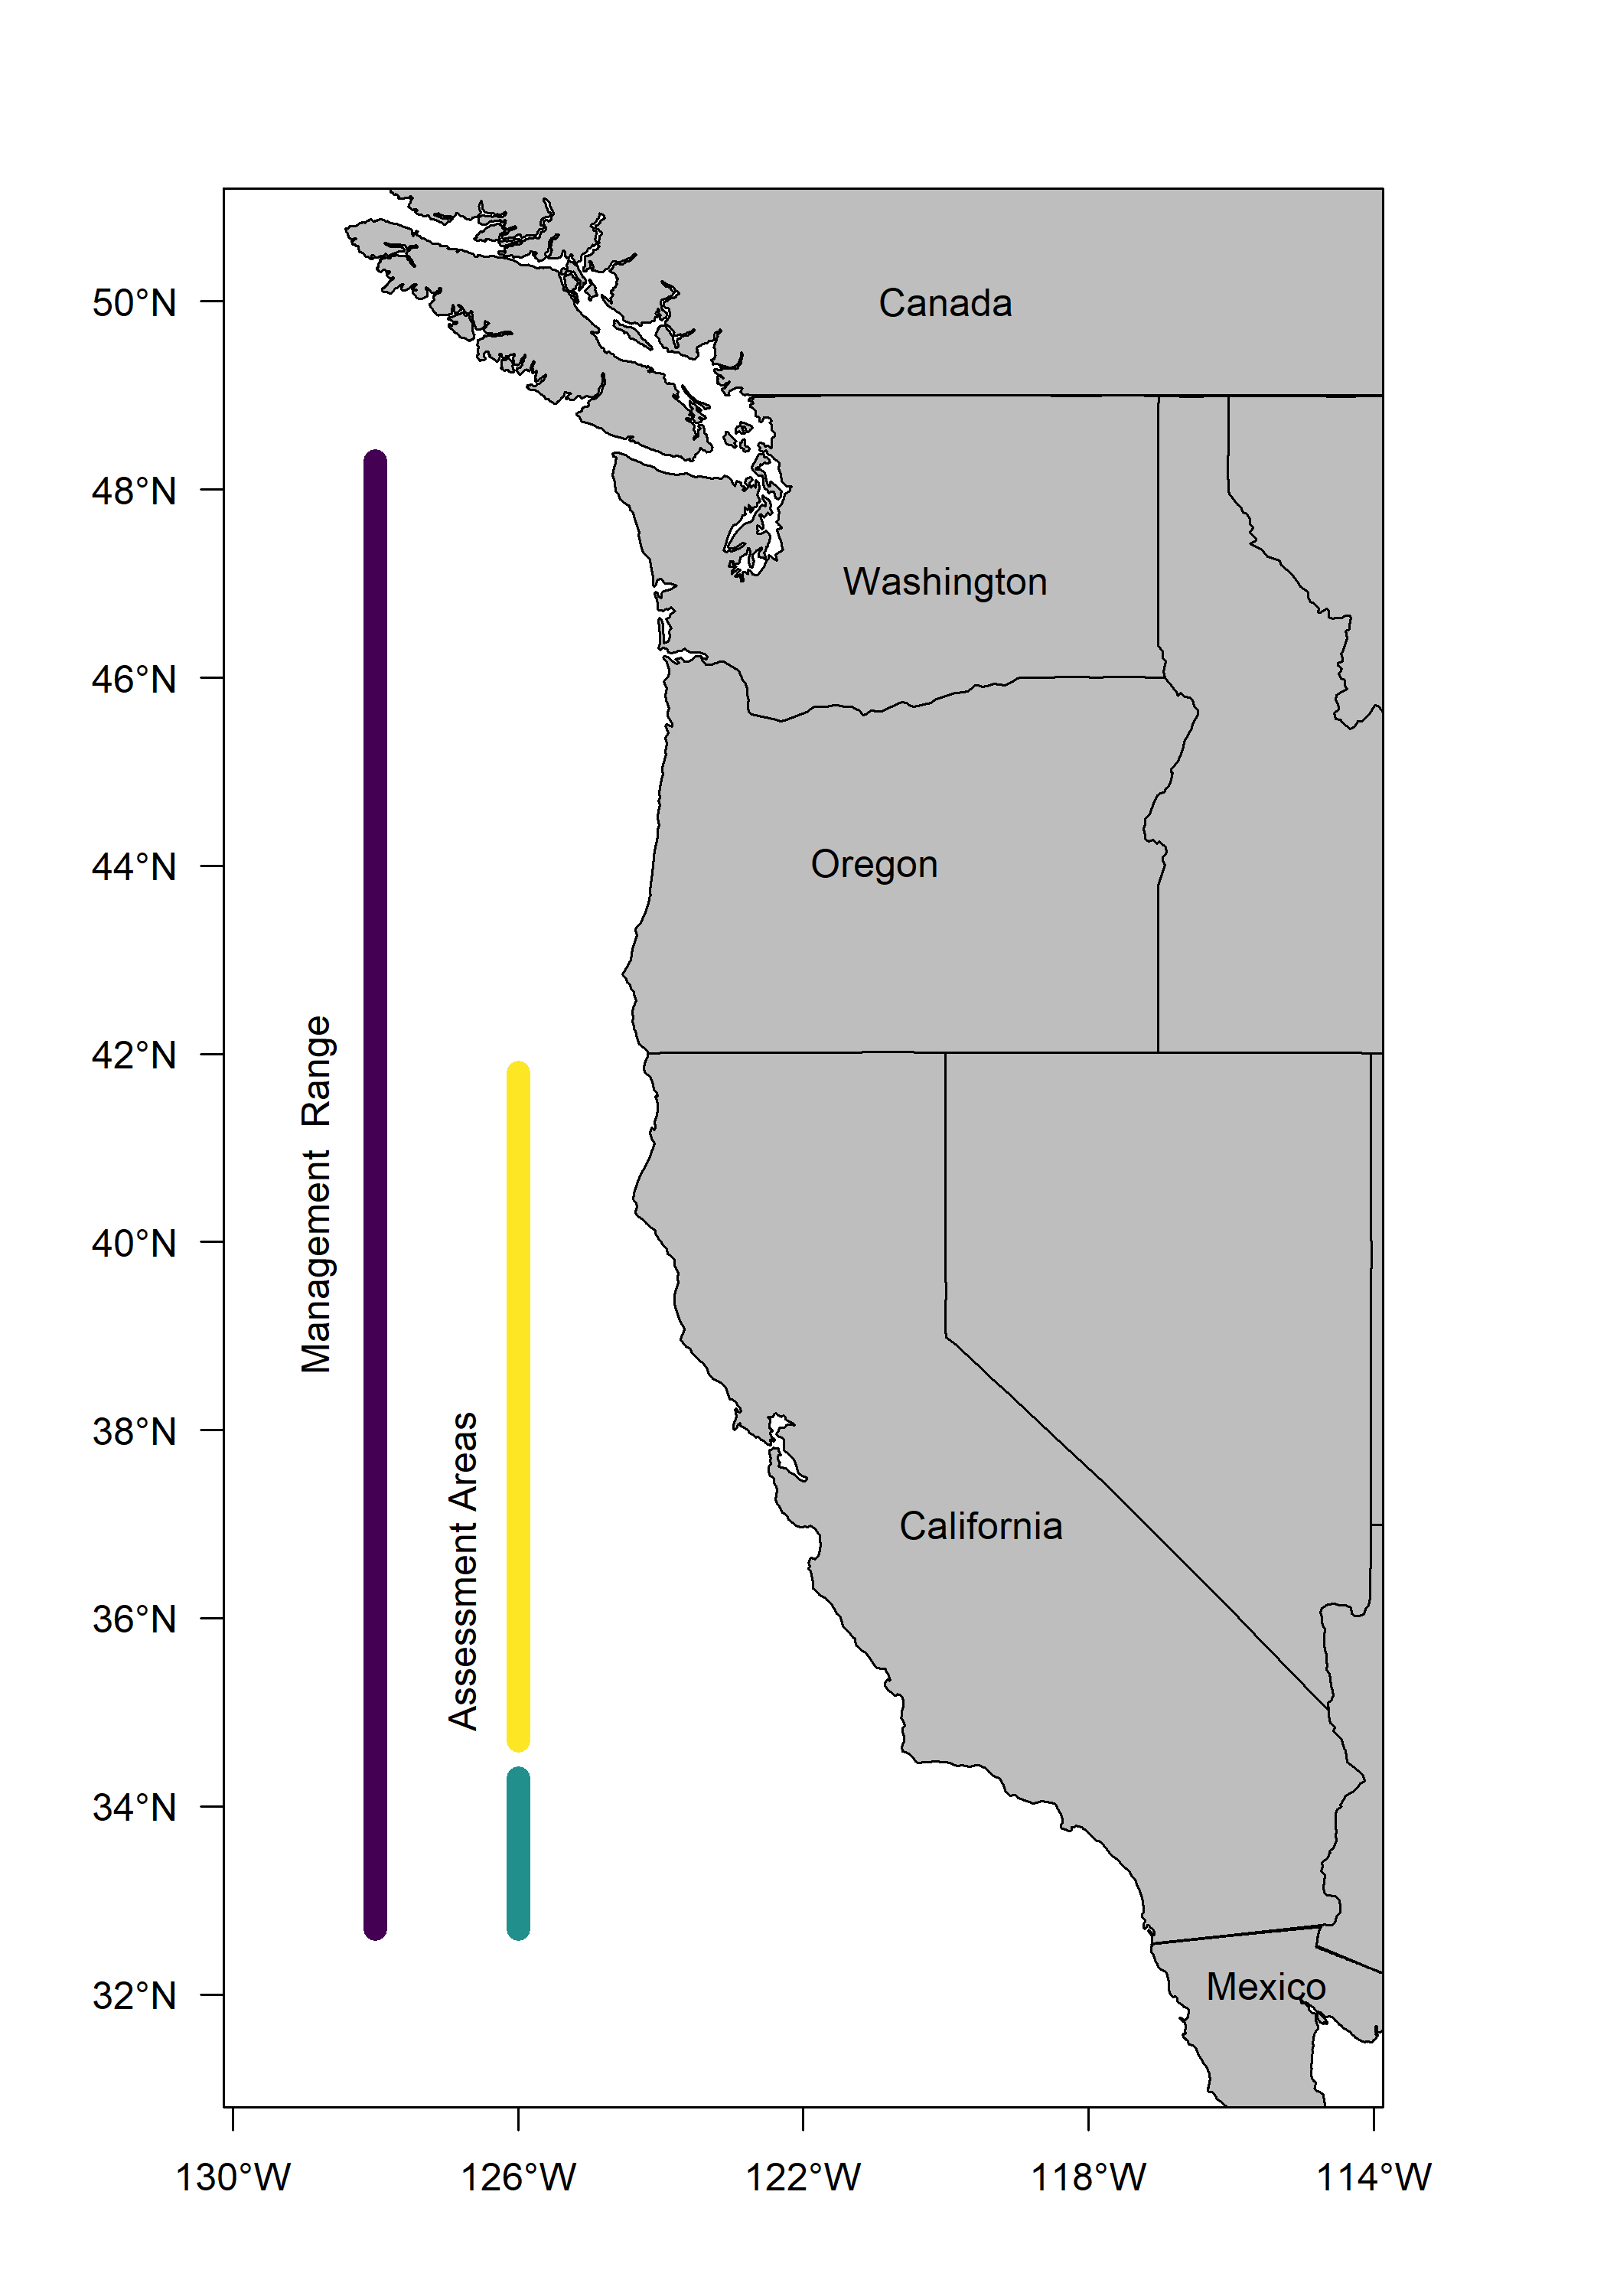
\includegraphics[width=1\textwidth,height=1\textheight]{C:/Assessments/2023/copper_rockfish_2023/documents/shared_figures/map.png}
\caption{Map of management area and the 2023 assessments areas for copper rockfish.\label{fig:ca-map}}
\end{figure}

\pagebreak

\begin{figure}
\centering
\includegraphics[width=1\textwidth,height=1\textheight]{N:/Assessments/CurrentAssessments/copper_rockfish_2023/models/sca/14.0_base/plots/catch2 landings stacked.png}
\caption{Landings by fleet used in the base model where catches in metric tons by fleet are stacked.\label{fig:catch}}
\end{figure}

\pagebreak

\begin{figure}
\centering
\includegraphics[width=1\textwidth,height=1\textheight]{N:/Assessments/CurrentAssessments/copper_rockfish_2023/models/sca/14.0_base/plots/data_plot.png}
\caption{Summary of data sources used in the base model.\label{fig:data-plot}}
\end{figure}

\pagebreak

\begin{figure}
\centering
\includegraphics[width=1\textwidth,height=1\textheight]{N:/Assessments/CurrentAssessments/copper_rockfish_2023/models/sca/14.0_base/plots/comp_lendat_bubflt1mkt0.png}
\caption{Length composition data from the commercial dead fleet.\label{fig:com-dead-len-data}}
\end{figure}

\pagebreak

\begin{figure}
\centering
\includegraphics[width=1\textwidth,height=1\textheight]{N:/Assessments/CurrentAssessments/copper_rockfish_2023/models/sca/14.0_base/plots/comp_lendat_data_weighting_TA1.8_Commercial_dead.png}
\caption{Mean length for commercial dead fleet with 95 percent confidence intervals.\label{fig:mean-com-dead-len-data}}
\end{figure}

\pagebreak

\begin{figure}
\centering
\includegraphics[width=1\textwidth,height=1\textheight]{N:/Assessments/CurrentAssessments/copper_rockfish_2023/models/sca/14.0_base/plots/comp_lendat_data_weighting_TA1.8_Commercial_dead.png}
\caption{Age composition data from the commercial dead and recreational CPFV fleets. The commercial samples were all from 2022 and the CPFV samples were all from 1975.\label{fig:com-dead-age-data}}
\end{figure}

\pagebreak

\begin{figure}
\centering
\includegraphics[width=1\textwidth,height=1\textheight]{N:/Assessments/CurrentAssessments/copper_rockfish_2023/data/ages/plots/coop_crfs_length_comparison.png}
\caption{Comparison of all length collected by the CRFS sampling program for the CPFV fleet to the lengths from the fish with ages from the cooperative sampling program. The length distributions in the area north of Point Conception are in general agreement while the distribution of lengths collected by this program does not align with the length samples from CRFS.\label{fig:coop-len-comparison}}
\end{figure}

\pagebreak

\begin{figure}
\centering
\includegraphics[width=1\textwidth,height=1\textheight]{N:/Assessments/CurrentAssessments/copper_rockfish_2023/models/sca/14.0_base/plots/comp_lendat_bubflt2mkt0.png}
\caption{Length composition data from the commercial live fleet.\label{fig:com-live-len-data}}
\end{figure}

\pagebreak

\begin{figure}
\centering
\includegraphics[width=1\textwidth,height=1\textheight]{N:/Assessments/CurrentAssessments/copper_rockfish_2023/models/sca/14.0_base/plots/comp_lendat_data_weighting_TA1.8_Commercial_live.png}
\caption{Mean length for commercial live fleet with 95 percent confidence intervals.\label{fig:mean-com-live-len-data}}
\end{figure}

\pagebreak

\begin{figure}
\centering
\includegraphics[width=1\textwidth,height=1\textheight]{N:/Assessments/CurrentAssessments/copper_rockfish_2023/data/rec_indices/mrfss_cpfv_dockside/south/forSS/Index.png}
\caption{Estimated annual index of abundances for the CPFV fleet based on MRFSS survey data.\label{fig:mrfss-index-main}}
\end{figure}

\pagebreak

\begin{figure}
\centering
\includegraphics[width=1\textwidth,height=1\textheight]{N:/Assessments/CurrentAssessments/copper_rockfish_2023/data/rec_indices/crfs_cpfv_onboard/south/main_effects/Index.png}
\caption{Estimated annual index of abundances for the CPFV fleet based on CRFS survey data.\label{fig:crfs-index-main}}
\end{figure}

\pagebreak

\begin{figure}
\centering
\includegraphics[width=1\textwidth,height=1\textheight]{N:/Assessments/CurrentAssessments/copper_rockfish_2023/data/rec_indices/crfs_pr_dockside/south/rm_last2yrs/Index.png}
\caption{Estimated annual index of abundances for the CPFV fleet based on CRFS survey data.\label{fig:crfs-pr-index-main}}
\end{figure}

\pagebreak

\begin{figure}
\centering
\includegraphics[width=1\textwidth,height=1\textheight]{N:/Assessments/CurrentAssessments/copper_rockfish_2023/models/sca/14.0_base/plots/comp_lendat_bubflt3mkt0_page2.png}
\caption{Length composition data from the recreational CPFV fleet.\label{fig:rec-cpfv-len-data}}
\end{figure}

\pagebreak

\begin{figure}
\centering
\includegraphics[width=1\textwidth,height=1\textheight]{N:/Assessments/CurrentAssessments/copper_rockfish_2023/models/sca/14.0_base/plots/comp_lendat_data_weighting_TA1.8_Rec_CPFV.png}
\caption{Mean length for recreational CPFV fleet with 95 percent confidence intervals.\label{fig:mean-rec-cpfv-len-data}}
\end{figure}

\pagebreak

\begin{figure}
\centering
\includegraphics[width=1\textwidth,height=1\textheight]{N:/Assessments/CurrentAssessments/copper_rockfish_2023/models/sca/14.0_base/plots/comp_lendat_bubflt4mkt0_page2.png}
\caption{Length composition data from the recreation PR fleet.\label{fig:rec-pr-len-data}}
\end{figure}

\pagebreak

\begin{figure}
\centering
\includegraphics[width=1\textwidth,height=1\textheight]{N:/Assessments/CurrentAssessments/copper_rockfish_2023/models/sca/14.0_base/plots/comp_lendat_data_weighting_TA1.8_Rec_Private.png}
\caption{Mean length for recreational PR fleet with 95 percent confidence intervals.\label{fig:mean-rec-pr-len-data}}
\end{figure}

\pagebreak

\begin{figure}
\centering
\includegraphics[width=1\textwidth,height=1\textheight]{N:/Assessments/CurrentAssessments/copper_rockfish_2023/data/survey_indices/plots/south_survey_locations_designation.png}
\caption{Sample locations by each of the fishery-independent data sources used in the base model with indices of abundance, lengths, and ages if collected.\label{fig:survey-locations}}
\end{figure}

\pagebreak

\begin{figure}
\centering
\includegraphics[width=1\textwidth,height=1\textheight]{N:/Assessments/CurrentAssessments/copper_rockfish_2023/data/survey_indices/plots/south_survey_locations.png}
\caption{Sample locations by area, areas open to fishing (reference) and MPAS, for each of the fishery-independent data sources used in the base model with indices of abundance, lengths, and ages if collected.\label{fig:ref-mpa}}
\end{figure}

\pagebreak

\begin{figure}
\centering
\includegraphics[width=1\textwidth,height=1\textheight]{N:/Assessments/CurrentAssessments/copper_rockfish_2023/data/survey_indices/ccfrp/south/area_weighted/Index.png}
\caption{Estimated index of abundance from the CCFRP survey.\label{fig:ccfrp-index-main}}
\end{figure}

\pagebreak

\begin{figure}
\centering
\includegraphics[width=1\textwidth,height=1\textheight]{N:/Assessments/CurrentAssessments/copper_rockfish_2023/models/sca/14.0_base/plots/comp_lendat_bubflt5mkt0.png}
\caption{Length composition data from the CCFRP survey.\label{fig:ccfrp-len-data}}
\end{figure}

\pagebreak

\begin{figure}
\centering
\includegraphics[width=1\textwidth,height=1\textheight]{N:/Assessments/CurrentAssessments/copper_rockfish_2023/models/sca/14.0_base/plots/comp_gstagedat_bubflt5mkt0.png}
\caption{Age composition data from the CCFRP survey.\label{fig:ccfrp-age-data}}
\end{figure}

\pagebreak

\begin{figure}
\centering
\includegraphics[width=1\textwidth,height=1\textheight]{N:/Assessments/CurrentAssessments/copper_rockfish_2023/models/sca/14.0_base/plots/comp_lendat_data_weighting_TA1.8_CCFRP.png}
\caption{Mean length for the CCFRP survey with 95 percent confidence intervals.\label{fig:ccfrp-mean-len-data}}
\end{figure}

\pagebreak

\begin{figure}
\centering
\includegraphics[width=1\textwidth,height=1\textheight]{N:/Assessments/CurrentAssessments/copper_rockfish_2023/data/survey_indices/nwfsc_hkl/maps/Map_HL_Sites_lndscp.jpg}
\caption{Area sampled by the NWFSC Hook and Line survey.\label{fig:nwfsc-hkl-map}}
\end{figure}

\pagebreak

\begin{figure}
\centering
\includegraphics[width=1\textwidth,height=1\textheight]{N:/Assessments/CurrentAssessments/copper_rockfish_2023/data/survey_indices/nwfsc_hkl/plots/hkl_copper_by_site_count_all_years.png}
\caption{Observations of copper rockfish by the NWFSC Hook and Line survey by sample area, inside and outside Cowcod Conservation areas (CCA).\label{fig:nwfsc-hkl-site}}
\end{figure}

\pagebreak

\begin{figure}
\centering
\includegraphics[width=1\textwidth,height=1\textheight]{N:/Assessments/CurrentAssessments/copper_rockfish_2023/data/survey_indices/nwfsc_hkl/plots/standardized_cpue_nwfsc_hkl_inside_outside.png}
\caption{Standardized CPUE inside and outside the CCA.\label{fig:nwfsc-hkl-cca-main}}
\end{figure}

\pagebreak

\begin{figure}
\centering
\includegraphics[width=1\textwidth,height=1\textheight]{N:/Assessments/CurrentAssessments/copper_rockfish_2023/data/survey_indices/nwfsc_hkl/plots/nwfsc_hkl_observations_by_depth.png}
\caption{Number of observations by depth (m) inside and outside the CCAs.\label{fig:nwfsc-hkl-depth}}
\end{figure}

\pagebreak

\begin{figure}
\centering
\includegraphics[width=1\textwidth,height=1\textheight]{N:/Assessments/CurrentAssessments/copper_rockfish_2023/data/survey_indices/nwfsc_hkl/rstan_full_nb_glm_year_site_drop_swell_vermilion/Index.png}
\caption{Estimated index of abundance for copper rockfish.\label{fig:nwfsc-hkl-index-main}}
\end{figure}

\pagebreak

\begin{figure}
\centering
\includegraphics[width=1\textwidth,height=1\textheight]{N:/Assessments/CurrentAssessments/copper_rockfish_2023/data/survey_indices/nwfsc_hkl/plots/hkl_observations_by_length_sex_area.png}
\caption{Observed length (cm) distribution of copper rockfish by the NWFSC Hook and Line survey by sample area, inside and outside Cowcod Conservation areas (CCA).\label{fig:nwfsc-hkl-site-len}}
\end{figure}

\pagebreak

\begin{figure}
\centering
\includegraphics[width=1\textwidth,height=1\textheight]{N:/Assessments/CurrentAssessments/copper_rockfish_2023/data/survey_indices/nwfsc_hkl/plots/nwfsc_hkl_age_at_length.png}
\caption{Age and length by sex for copper rockfish in the NWFSC Hook and Line survey.\label{fig:nwfsc-hkl-len-age}}
\end{figure}

\pagebreak

\begin{figure}
\centering
\includegraphics[width=1\textwidth,height=1\textheight]{N:/Assessments/CurrentAssessments/copper_rockfish_2023/models/sca/14.0_base/plots/comp_lendat_bubflt7mkt0.png}
\caption{Length composition data from the NWFSC Hook and Line survey.\label{fig:hkl-len-data}}
\end{figure}

\pagebreak

\includegraphics[width=1\textwidth,height=1\textheight]{N:/Assessments/CurrentAssessments/copper_rockfish_2023/models/sca/14.0_base/plots/comp_lendat_data_weighting_TA1.8_NWFSC_HKL.png} \pagebreak

\begin{figure}
\centering
\includegraphics[width=1\textwidth,height=1\textheight]{N:/Assessments/CurrentAssessments/copper_rockfish_2023/data/survey_indices/rov/plots/rov_transect_collapsed_copper_south_protection_count.png}
\caption{The location and size of observations across all years and transects.\label{fig:rov-obs-loc}}
\end{figure}

\pagebreak

\begin{figure}
\centering
\includegraphics[width=1\textwidth,height=1\textheight]{N:/Assessments/CurrentAssessments/copper_rockfish_2023/data/survey_indices/rov/plots/south_raw_cpue_by_mpa_group_by_year.png}
\caption{The trend of the calculated CPUE by each MPA and Reference group by year.\label{fig:rov-raw-cpue}}
\end{figure}

\pagebreak

\begin{figure}
\centering
\includegraphics[width=1\textwidth,height=1\textheight]{N:/Assessments/CurrentAssessments/copper_rockfish_2023/data/survey_indices/rov/plots/rov_length_by_area_designation_april_data.png}
\caption{The distribution of lengths across all years for MPA and Reference areas north and south of Point Conception.\label{fig:rov-len}}
\end{figure}

\pagebreak

\begin{figure}
\centering
\includegraphics[width=1\textwidth,height=1\textheight]{N:/Assessments/CurrentAssessments/copper_rockfish_2023/models/sca/14.0_base/plots/comp_lendat_bubflt6mkt0.png}
\caption{Length composition data from the CDFW ROV survey.\label{fig:rov-len-data}}
\end{figure}

\pagebreak

\begin{figure}
\centering
\includegraphics[width=1\textwidth,height=1\textheight]{N:/Assessments/CurrentAssessments/copper_rockfish_2023/models/sca/14.0_base/plots/comp_lendat_data_weighting_TA1.8_CDFW_ROV.png}
\caption{Mean length for the CDFW ROV survey with 95 percent confidence intervals.\label{fig:mean-rov-len-data}}
\end{figure}

\pagebreak

\begin{figure}
\centering
\includegraphics[width=1\textwidth,height=1\textheight]{N:/Assessments/CurrentAssessments/copper_rockfish_2023/data/ages/plots/south_growth_length_comparison.png}
\caption{Length distribution of fish by collection source that were used as conditional age-at-length data in the growth fleet.\label{fig:growth-len-dist}}
\end{figure}

\pagebreak

\includegraphics[width=1\textwidth,height=1\textheight]{N:/Assessments/CurrentAssessments/copper_rockfish_2023/data/ages/plots/south_growth_age_comparison.png} \pagebreak

\begin{figure}
\centering
\includegraphics[width=1\textwidth,height=1\textheight]{N:/Assessments/CurrentAssessments/copper_rockfish_2023/data/wcgbt/south/plots/cpue_map.png}
\caption{Location and catch-per-unit-effort by location caught south of Point Conception by the NWFSC WCGBT survey.\label{fig:wcgbt-cpue}}
\end{figure}

\pagebreak

\begin{figure}
\centering
\includegraphics[width=1\textwidth,height=1\textheight]{N:/Assessments/CurrentAssessments/copper_rockfish_2023/data/wcgbt/south/plots/presence-absence_proportion_by_depth.png}
\caption{Number of positive tows across all years by depth in meters.\label{fig:wcgbt-depth}}
\end{figure}

\pagebreak

\begin{figure}
\centering
\includegraphics[width=1\textwidth,height=1\textheight]{N:/Assessments/CurrentAssessments/copper_rockfish_2023/data/wcgbt/plots/wcgbt_south_age_at_length_by_area.png}
\caption{Age and length by sex for copper rockfish caught south of Point Conception by the NWFSC WCGBT survey.\label{fig:wcgbt-len-age}}
\end{figure}

\pagebreak

\hypertarget{biology}{%
\subsection{Biology}\label{biology}}

\begin{figure}
\centering
\includegraphics[width=1\textwidth,height=1\textheight]{C:/Assessments/2023/copper_rockfish_2023/documents/shared_figures/copper_length_by_half_month.png}
\caption{Distribution of YOY copper rockfish lengths from fish genetically identified from D. Baetscher.\label{fig:copper-smurf-length}}
\end{figure}

\pagebreak

\begin{figure}
\centering
\includegraphics[width=1\textwidth,height=1\textheight]{N:/Assessments/CurrentAssessments/copper_rockfish_2023/models/sca/14.0_base/plots/bio6_maturity.png}
\caption{Maturity as a function of length.\label{fig:maturity}}
\end{figure}

\pagebreak

\begin{figure}
\centering
\includegraphics[width=1\textwidth,height=1\textheight]{N:/Assessments/CurrentAssessments/copper_rockfish_2023/models/sca/14.0_base/plots/bio9_fecundity_len.png}
\caption{Fecundity as a function of length.\label{fig:fecundity}}
\end{figure}

\pagebreak

\begin{figure}
\centering
\includegraphics[width=1\textwidth,height=1\textheight]{N:/Assessments/CurrentAssessments/copper_rockfish_2023/data/wcgbt/plots/length_fraction_female.png}
\caption{Fraction of each sex by length by the NWFSC WCGBT survey.\label{fig:frac-sex-len}}
\end{figure}

\pagebreak

\begin{figure}
\centering
\includegraphics[width=1\textwidth,height=1\textheight]{N:/Assessments/CurrentAssessments/copper_rockfish_2023/data/biology/plots/Length_Weight_All.png}
\caption{Estimated weight-at-length.\label{fig:weight-length}}
\end{figure}

\pagebreak

\begin{figure}
\centering
\includegraphics[width=1\textwidth,height=1\textheight]{N:/Assessments/CurrentAssessments/copper_rockfish_2023/data/ages/ageing_error/B0_S3/Reader_1_vs_Reader_2.png}
\caption{Distribution of double reads between age reader 1 and 2.\label{fig:age-error-dist}}
\end{figure}

\pagebreak

\begin{figure}
\centering
\includegraphics[width=1\textwidth,height=1\textheight]{N:/Assessments/CurrentAssessments/copper_rockfish_2023/models/sca/14.0_base/plots/numbers5_ageerrorSD.png}
\caption{Ageing imprecision standard deviation of observed age in years.\label{fig:age-error}}
\end{figure}

\pagebreak

\begin{figure}
\centering
\includegraphics[width=1\textwidth,height=1\textheight]{N:/Assessments/CurrentAssessments/copper_rockfish_2023/models/sca/14.0_base/plots/numbers10_ageerror_matrix_1.png}
\caption{Distribution of observed age at true age for ageing error type 1.\label{fig:age-error-matrix}}
\end{figure}

\pagebreak

\hypertarget{model-results}{%
\subsection{Model Results}\label{model-results}}

\hypertarget{bridging}{%
\subsubsection{Bridging}\label{bridging}}

\begin{figure}
\centering
\includegraphics[width=1\textwidth,height=1\textheight]{N:/Assessments/CurrentAssessments/copper_rockfish_2023/models/sca/_bridging/_plots/0_model_convert_compare2_spawnbio_uncertainty.png}
\caption{Model version bridge comparison of estimated spawning output.\label{fig:bridge-ssb}}
\end{figure}

\pagebreak

\begin{figure}
\centering
\includegraphics[width=1\textwidth,height=1\textheight]{N:/Assessments/CurrentAssessments/copper_rockfish_2023/models/sca/_bridging/_plots/0_model_convert_compare4_Bratio_uncertainty.png}
\caption{Model version bridge comparison of estimated fraction unfished.\label{fig:bridge-depl}}
\end{figure}

\pagebreak

\begin{figure}
\centering
\includegraphics[width=1\textwidth,height=1\textheight]{N:/Assessments/CurrentAssessments/copper_rockfish_2023/models/sca/_bridging/_plots/full_bridge_1_compare2_spawnbio_uncertainty.png}
\caption{Model structure and data bridging comparison of estimated spawning output.\label{fig:data-bridge-ssb-1}}
\end{figure}

\pagebreak

\begin{figure}
\centering
\includegraphics[width=1\textwidth,height=1\textheight]{N:/Assessments/CurrentAssessments/copper_rockfish_2023/models/sca/_bridging/_plots/full_bridge_1_compare4_Bratio_uncertainty.png}
\caption{Model structure and data bridging comparison of estimated fraction unfished.\label{fig:data-bridge-depl-1}}
\end{figure}

\pagebreak

\begin{figure}
\centering
\includegraphics[width=1\textwidth,height=1\textheight]{N:/Assessments/CurrentAssessments/copper_rockfish_2023/models/sca/_bridging/_plots/full_bridge_2_compare2_spawnbio_uncertainty.png}
\caption{Model structure and data bridging comparison of estimated spawning output.\label{fig:data-bridge-ssb-2}}
\end{figure}

\pagebreak

\begin{figure}
\centering
\includegraphics[width=1\textwidth,height=1\textheight]{N:/Assessments/CurrentAssessments/copper_rockfish_2023/models/sca/_bridging/_plots/full_bridge_2_compare4_Bratio_uncertainty.png}
\caption{Model structure and data bridging comparison of estimated fraction unfished.\label{fig:data-bridge-depl-2}}
\end{figure}

\pagebreak

\hypertarget{biology-1}{%
\subsubsection{Biology}\label{biology-1}}

\begin{figure}
\centering
\includegraphics[width=1\textwidth,height=1\textheight]{N:/Assessments/CurrentAssessments/copper_rockfish_2023/models/sca/14.0_base/plots/bio1_sizeatage.png}
\caption{Model estimated length-at-age in the beginning of the year. Shaded area indicates 95 percent distribution of length-at-age around the estimated growth curve.\label{fig:mod-est-len-age}}
\end{figure}

\pagebreak

\hypertarget{selectivity}{%
\subsubsection{Selectivity}\label{selectivity}}

\hypertarget{recruitment-1}{%
\subsubsection{Recruitment}\label{recruitment-1}}

\begin{figure}
\centering
\includegraphics[width=1\textwidth,height=1\textheight]{N:/Assessments/CurrentAssessments/copper_rockfish_2023/models/sca/14.0_base/plots/ts11_Age-0_recruits_(1000s)_with_95_asymptotic_intervals.png}
\caption{Estimated time series of age-0 recruits (1000s).\label{fig:recruits}}
\end{figure}

\pagebreak

\begin{figure}
\centering
\includegraphics[width=1\textwidth,height=1\textheight]{N:/Assessments/CurrentAssessments/copper_rockfish_2023/models/sca/14.0_base/plots/recdevs2_withbars.png}
\caption{Estimated time series of recruitment deviations.\label{fig:rec-devs}}
\end{figure}

\pagebreak

\begin{figure}
\centering
\includegraphics[width=1\textwidth,height=1\textheight]{N:/Assessments/CurrentAssessments/copper_rockfish_2023/models/sca/14.0_base/plots/SR_curve.png}
\caption{Stock-recruit curve. Point colors indicate year, with warmer colors indicating earlier years and cooler colors in showing later years.\label{fig:bh-curve}}
\end{figure}

\pagebreak

\hypertarget{fits-to-data}{%
\subsubsection{Fits to Data}\label{fits-to-data}}

\begin{figure}
\centering
\includegraphics[width=1\textwidth,height=1\textheight]{N:/Assessments/CurrentAssessments/copper_rockfish_2023/models/sca/14.0_base/plots/comp_lenfit_residsflt1mkt0.png}
\caption{Pearson residuals for commercial fleet. Closed bubble are positive residuals (observed \textgreater{} expected) and open bubbles are negative residuals (observed \textless{} expected).\label{fig:com-dead-pearson}}
\end{figure}

\pagebreak

\begin{figure}
\centering
\includegraphics[width=1\textwidth,height=1\textheight]{N:/Assessments/CurrentAssessments/copper_rockfish_2023/models/sca/14.0_base/plots/comp_lenfit_data_weighting_TA1.8_Commercial_dead.png}
\caption{Mean length for commercial dead lengths with 95 percent confidence intervals based on current samples sizes.\label{fig:com-dead-mean-len-fit}}
\end{figure}

\pagebreak

\begin{figure}
\centering
\includegraphics[width=1\textwidth,height=1\textheight]{N:/Assessments/CurrentAssessments/copper_rockfish_2023/models/sca/14.0_base/plots/comp_agefit__aggregated_across_time.png}
\caption{Age composition data aggregated across time by fleet.\label{fig:agg-marg-age-fit}}
\end{figure}

\pagebreak

\begin{figure}
\centering
\includegraphics[width=1\textwidth,height=1\textheight]{N:/Assessments/CurrentAssessments/copper_rockfish_2023/models/sca/14.0_base/plots/comp_agefit_residsflt1mkt0.png}
\caption{Pearson residuals for commercial dead age data. Closed bubble are positive residuals (observed \textgreater{} expected) and open bubbles are negative residuals (observed \textless{} expected).\label{fig:com-dead-age-pearson}}
\end{figure}

\pagebreak

\begin{figure}
\centering
\includegraphics[width=1\textwidth,height=1\textheight]{N:/Assessments/CurrentAssessments/copper_rockfish_2023/models/sca/14.0_base/plots/comp_lenfit_residsflt2mkt0.png}
\caption{Pearson residuals for commercial live fleet. Closed bubble are positive residuals (observed \textgreater{} expected) and open bubbles are negative residuals (observed \textless{} expected).\label{fig:com-live-pearson}}
\end{figure}

\pagebreak

\begin{figure}
\centering
\includegraphics[width=1\textwidth,height=1\textheight]{N:/Assessments/CurrentAssessments/copper_rockfish_2023/models/sca/14.0_base/plots/comp_lenfit_data_weighting_TA1.8_Commercial_live.png}
\caption{Mean length for commercial live fish lengths with 95 percent confidence intervals based on current samples sizes.\label{fig:com-live-mean-len-fit}}
\end{figure}

\pagebreak

\begin{figure}
\centering
\includegraphics[width=1\textwidth,height=1\textheight]{N:/Assessments/CurrentAssessments/copper_rockfish_2023/models/sca/14.0_base/plots/comp_lenfit_residsflt3mkt0_page2.png}
\caption{Pearson residuals for recreational CPFV fleet. Closed bubble are positive residuals (observed \textgreater{} expected) and open bubbles are negative residuals (observed \textless{} expected).\label{fig:rec-cpfv-pearson}}
\end{figure}

\pagebreak

\begin{figure}
\centering
\includegraphics[width=1\textwidth,height=1\textheight]{N:/Assessments/CurrentAssessments/copper_rockfish_2023/models/sca/14.0_base/plots/comp_lenfit_data_weighting_TA1.8_Rec_CPFV.png}
\caption{Mean length for recreational CPFV lengths with 95 percent confidence intervals based on current samples sizes.\label{fig:rec-cpfv-mean-len-fit}}
\end{figure}

\pagebreak

\begin{figure}
\centering
\includegraphics[width=1\textwidth,height=1\textheight]{N:/Assessments/CurrentAssessments/copper_rockfish_2023/models/sca/14.0_base/plots/comp_agefit_residsflt3mkt0.png}
\caption{Pearson residuals for recreational CPFV age data. Closed bubble are positive residuals (observed \textgreater{} expected) and open bubbles are negative residuals (observed \textless{} expected).\label{fig:rec-cpfv-age-pearson}}
\end{figure}

\pagebreak

\begin{figure}
\centering
\includegraphics[width=1\textwidth,height=1\textheight]{N:/Assessments/CurrentAssessments/copper_rockfish_2023/models/sca/14.0_base/plots/comp_lenfit_residsflt4mkt0_page2.png}
\caption{Pearson residuals for recreational private/rental fleet. Closed bubble are positive residuals (observed \textgreater{} expected) and open bubbles are negative residuals (observed \textless{} expected).\label{fig:rec-pr-pearson}}
\end{figure}

\pagebreak

\begin{figure}
\centering
\includegraphics[width=1\textwidth,height=1\textheight]{N:/Assessments/CurrentAssessments/copper_rockfish_2023/models/sca/14.0_base/plots/comp_lenfit_data_weighting_TA1.8_Rec_Private.png}
\caption{Mean length for recreational private/rental lengths with 95 percent confidence intervals based on current samples sizes.\label{fig:rec-pr-mean-len-fit}}
\end{figure}

\pagebreak

\begin{figure}
\centering
\includegraphics[width=1\textwidth,height=1\textheight]{N:/Assessments/CurrentAssessments/copper_rockfish_2023/models/sca/14.0_base/plots/comp_lenfit_residsflt5mkt0.png}
\caption{Pearson residuals for CCFRP survey length data. Closed bubble are positive residuals (observed \textgreater{} expected) and open bubbles are negative residuals (observed \textless{} expected).\label{fig:ccfrp-len-pearson}}
\end{figure}

\pagebreak

\begin{figure}
\centering
\includegraphics[width=1\textwidth,height=1\textheight]{N:/Assessments/CurrentAssessments/copper_rockfish_2023/models/sca/14.0_base/plots/comp_lenfit_data_weighting_TA1.8_CCFRP.png}
\caption{Mean length for CCFRP survey lengths with 95 percent confidence intervals based on current samples sizes.\label{fig:ccfrp-mean-len-fit}}
\end{figure}

\pagebreak

\begin{figure}
\centering
\includegraphics[width=1\textwidth,height=1\textheight]{N:/Assessments/CurrentAssessments/copper_rockfish_2023/models/sca/14.0_base/plots/comp_condAAlfit_residsflt5mkt0.png}
\caption{Pearson residuals for CCFRP survey conditional-age-at-length data. Closed bubble are positive residuals (observed \textgreater{} expected) and open bubbles are negative residuals (observed \textless{} expected).\label{fig:ccfrp-age-pearson}}
\end{figure}

\pagebreak

\begin{figure}
\centering
\includegraphics[width=1\textwidth,height=1\textheight]{N:/Assessments/CurrentAssessments/copper_rockfish_2023/models/sca/14.0_base/plots/comp_lenfit_residsflt6mkt0.png}
\caption{Pearson residuals for CDFW ROV survey length data. Closed bubble are positive residuals (observed \textgreater{} expected) and open bubbles are negative residuals (observed \textless{} expected).\label{fig:rov-pearson}}
\end{figure}

\pagebreak

\begin{figure}
\centering
\includegraphics[width=1\textwidth,height=1\textheight]{N:/Assessments/CurrentAssessments/copper_rockfish_2023/models/sca/14.0_base/plots/comp_lenfit_data_weighting_TA1.8_CDFW_ROV.png}
\caption{Mean length for CDFW ROV survey lengths with 95 percent confidence intervals based on current samples sizes.\label{fig:rov-mean-len-fit}}
\end{figure}

\pagebreak

\begin{figure}
\centering
\includegraphics[width=1\textwidth,height=1\textheight]{N:/Assessments/CurrentAssessments/copper_rockfish_2023/models/sca/14.0_base/plots/comp_lenfit_residsflt7mkt0.png}
\caption{Pearson residuals for NWFSC Hook and Line survey length data. Closed bubble are positive residuals (observed \textgreater{} expected) and open bubbles are negative residuals (observed \textless{} expected).\label{fig:nwfsc-hkl-pearson}}
\end{figure}

\pagebreak

\begin{figure}
\centering
\includegraphics[width=1\textwidth,height=1\textheight]{N:/Assessments/CurrentAssessments/copper_rockfish_2023/models/sca/14.0_base/plots/comp_lenfit_data_weighting_TA1.8_NWFSC_HKL.png}
\caption{Mean length for NWFSC Hook and Line survey lengths with 95 percent confidence intervals based on current samples sizes.\label{fig:nwfsc-hkl-mean-len-fit}}
\end{figure}

\pagebreak

\begin{figure}
\centering
\includegraphics[width=1\textwidth,height=1\textheight]{N:/Assessments/CurrentAssessments/copper_rockfish_2023/models/sca/14.0_base/plots/comp_condAALfit_residsflt7mkt0_page1.png}
\caption{Pearson residuals for NWFSC Hook and Line survey conditional-age-at-length data. Closed bubble are positive residuals (observed \textgreater{} expected) and open bubbles are negative residuals (observed \textless{} expected).\label{fig:nwfsc-hkl-age-pearson-1}}
\end{figure}

\pagebreak

\begin{figure}
\centering
\includegraphics[width=1\textwidth,height=1\textheight]{N:/Assessments/CurrentAssessments/copper_rockfish_2023/models/sca/14.0_base/plots/comp_condAALfit_residsflt7mkt0_page2.png}
\caption{Pearson residuals for NWFSC Hook and Line survey conditional-age-at-length data. Closed bubble are positive residuals (observed \textgreater{} expected) and open bubbles are negative residuals (observed \textless{} expected).\label{fig:nwfsc-hkl-age-pearson-2}}
\end{figure}

\pagebreak

\begin{figure}
\centering
\includegraphics[width=1\textwidth,height=1\textheight]{N:/Assessments/CurrentAssessments/copper_rockfish_2023/models/sca/14.0_base/plots/comp_condAALfit_residsflt7mkt0_page3.png}
\caption{Pearson residuals for NWFSC Hook and Line survey conditional-age-at-length data. Closed bubble are positive residuals (observed \textgreater{} expected) and open bubbles are negative residuals (observed \textless{} expected).\label{fig:nwfsc-hkl-age-pearson-3}}
\end{figure}

\pagebreak

\begin{figure}
\centering
\includegraphics[width=1\textwidth,height=1\textheight]{N:/Assessments/CurrentAssessments/copper_rockfish_2023/models/sca/14.0_base/plots/comp_condAALfit_data_weighting_TA1.8_condAgeNWFSC_HKL.png}
\caption{Mean age for NWFSC Hook and Line survey age data with 95 percent confidence intervals based on current samples sizes.\label{fig:nwfsc-hkl-mean-age-fit}}
\end{figure}

\pagebreak

\begin{figure}
\centering
\includegraphics[width=1\textwidth,height=1\textheight]{N:/Assessments/CurrentAssessments/copper_rockfish_2023/models/sca/14.0_base/plots/comp_condAALfit_residsflt9mkt0_page1.png}
\caption{Pearson residuals for the growth conditional-age-at-length data. Closed bubble are positive residuals (observed \textgreater{} expected) and open bubbles are negative residuals (observed \textless{} expected).\label{fig:growth-age-pearson-1}}
\end{figure}

\pagebreak

\begin{figure}
\centering
\includegraphics[width=1\textwidth,height=1\textheight]{N:/Assessments/CurrentAssessments/copper_rockfish_2023/models/sca/14.0_base/plots/comp_condAALfit_residsflt9mkt0_page2.png}
\caption{Pearson residuals for the growth conditional-age-at-length data. Closed bubble are positive residuals (observed \textgreater{} expected) and open bubbles are negative residuals (observed \textless{} expected).\label{fig:growth-age-pearson-2}}
\end{figure}

\pagebreak

\begin{figure}
\centering
\includegraphics[width=1\textwidth,height=1\textheight]{N:/Assessments/CurrentAssessments/copper_rockfish_2023/models/sca/14.0_base/plots/comp_condAALfit_residsflt9mkt0_page3.png}
\caption{Pearson residuals for the growth conditional-age-at-length data. Closed bubble are positive residuals (observed \textgreater{} expected) and open bubbles are negative residuals (observed \textless{} expected).\label{fig:growth-age-pearson-3}}
\end{figure}

\pagebreak

\begin{figure}
\centering
\includegraphics[width=1\textwidth,height=1\textheight]{N:/Assessments/CurrentAssessments/copper_rockfish_2023/models/sca/14.0_base/plots/comp_condAALfit_data_weighting_TA1.8_condAgeWCGBT_Growth.png}
\caption{Mean age for the growth age data with 95 percent confidence intervals based on current samples sizes.\label{fig:growth-mean-age-fit-wcgbt}}
\end{figure}

\pagebreak

\begin{figure}
\centering
\includegraphics[width=1\textwidth,height=1\textheight]{N:/Assessments/CurrentAssessments/copper_rockfish_2023/models/sca/14.0_base/plots/comp_condAALfit_data_weighting_TA1.8_condAgeCOOP_Growth.png}
\caption{Mean age for the growth age data with 95 percent confidence intervals based on current samples sizes.\label{fig:growth-mean-age-fit}}
\end{figure}

\pagebreak

\begin{figure}
\centering
\includegraphics[width=1\textwidth,height=1\textheight]{N:/Assessments/CurrentAssessments/copper_rockfish_2023/models/sca/14.0_base/plots/index5_logcpuefit_Rec_CPFV.png}
\caption{Fit to log index data on log scale for the recreational (MRFSS) CPFV index of abundance. Lines indicate 95\% uncertainty interval around index values based on the model assumption of lognormal error. Thicker lines (if present) indicate input uncertainty before addition of estimated additional uncertainty parameter.\label{fig:mrfss-cpfv-index-fit}}
\end{figure}

\pagebreak

\begin{figure}
\centering
\includegraphics[width=1\textwidth,height=1\textheight]{N:/Assessments/CurrentAssessments/copper_rockfish_2023/models/sca/14.0_base/plots/index5_logcpuefit_CRFS_CPFV.png}
\caption{Fit to log index data on log scale for the recreational CRFS CPFV index of abundance. Lines indicate 95\% uncertainty interval around index values based on the model assumption of lognormal error. Thicker lines (if present) indicate input uncertainty before addition of estimated additional uncertainty parameter.\label{fig:crfs-cpfv-index-fit}}
\end{figure}

\pagebreak

\begin{figure}
\centering
\includegraphics[width=1\textwidth,height=1\textheight]{N:/Assessments/CurrentAssessments/copper_rockfish_2023/models/sca/14.0_base/plots/index5_logcpuefit_Rec_Private.png}
\caption{Fit to log index data on log scale for the recreational private index of abundance. Lines indicate 95\% uncertainty interval around index values based on the model assumption of lognormal error. Thicker lines (if present) indicate input uncertainty before addition of estimated additional uncertainty parameter.\label{fig:crfs-pr-index-fit}}
\end{figure}

\pagebreak

\begin{figure}
\centering
\includegraphics[width=1\textwidth,height=1\textheight]{N:/Assessments/CurrentAssessments/copper_rockfish_2023/models/sca/14.0_base/plots/index5_logcpuefit_CCFRP.png}
\caption{Fit to log index data on log scale for the CCFRP index of abundance. Lines indicate 95\% uncertainty interval around index values based on the model assumption of lognormal error. Thicker lines (if present) indicate input uncertainty before addition of estimated additional uncertainty parameter.\label{fig:ccfrp-index-fit}}
\end{figure}

\pagebreak

\begin{figure}
\centering
\includegraphics[width=1\textwidth,height=1\textheight]{N:/Assessments/CurrentAssessments/copper_rockfish_2023/models/sca/14.0_base/plots/index5_logcpuefit_CDFW_ROV.png}
\caption{Fit to log index data on log scale for the CDFW ROV index of abundance. Lines indicate 95\% uncertainty interval around index values based on the model assumption of lognormal error. Thicker lines (if present) indicate input uncertainty before addition of estimated additional uncertainty parameter.\label{fig:rov-index-fit}}
\end{figure}

\pagebreak

\begin{figure}
\centering
\includegraphics[width=1\textwidth,height=1\textheight]{N:/Assessments/CurrentAssessments/copper_rockfish_2023/models/sca/14.0_base/plots/index5_logcpuefit_NWFSC_HKL.png}
\caption{Fit to log index data on log scale for the NWFSC Hook and Line index of abundance. Lines indicate 95\% uncertainty interval around index values based on the model assumption of lognormal error. Thicker lines (if present) indicate input uncertainty before addition of estimated additional uncertainty parameter.\label{fig:nwfsc-hkl-index-fit}}
\end{figure}

\pagebreak

\hypertarget{time-series}{%
\subsubsection{Time-series}\label{time-series}}

\begin{figure}
\centering
\includegraphics[width=1\textwidth,height=1\textheight]{N:/Assessments/CurrentAssessments/copper_rockfish_2023/models/sca/14.0_base/plots/ts7_Spawning_output_with_95_asymptotic_intervals_intervals.png}
\caption{Estimated time series of spawning biomass.\label{fig:ssb}}
\end{figure}

\pagebreak

\begin{figure}
\centering
\includegraphics[width=1\textwidth,height=1\textheight]{N:/Assessments/CurrentAssessments/copper_rockfish_2023/models/sca/14.0_base/plots/ts1_Total_biomass_(mt).png}
\caption{Estimated time series of total biomass.\label{fig:tot-bio}}
\end{figure}

\pagebreak

\begin{figure}
\centering
\includegraphics[width=1\textwidth,height=1\textheight]{N:/Assessments/CurrentAssessments/copper_rockfish_2023/models/sca/14.0_base/plots/ts9_Relative_spawning_output_intervals.png}
\caption{Estimated time series of fraction of unfished spawning biomass.\label{fig:depl}}
\end{figure}

\pagebreak

\hypertarget{sensitivity-analyses-and-retrospectives}{%
\subsubsection{Sensitivity Analyses and Retrospectives}\label{sensitivity-analyses-and-retrospectives}}

\hypertarget{likelihood-profiles-1}{%
\subsubsection{Likelihood Profiles}\label{likelihood-profiles-1}}

\hypertarget{reference-points-and-forecasts}{%
\subsubsection{Reference Points and Forecasts}\label{reference-points-and-forecasts}}

\begin{figure}
\centering
\includegraphics[width=1\textwidth,height=1\textheight]{N:/Assessments/CurrentAssessments/copper_rockfish_2023/models/sca/14.0_base/plots/SPR2_minusSPRseries.png}
\caption{Estimated 1 - relative spawning ratio (SPR) by year.\label{fig:1-spr}}
\end{figure}

\clearpage

\begin{figure}
\centering
\includegraphics[width=1\textwidth,height=1\textheight]{N:/Assessments/CurrentAssessments/copper_rockfish_2023/models/sca/14.0_base/plots/SPR4_phase.png}
\caption{Phase plot of the relative biomass (also referred to as fraction unfished) versus the SPR ratio where each point represents the biomass ratio at the start of the year and the relative fishing intensity in that same year. Lines through the final point show the 95 percent intervals based on the asymptotic uncertainty for each dimension. The shaded ellipse is a 95 percent region which accounts for the estimated correlations between the biomass ratio and SPR ratio.\label{fig:phase}}
\end{figure}

\pagebreak

\begin{figure}
\centering
\includegraphics[width=1\textwidth,height=1\textheight]{N:/Assessments/CurrentAssessments/copper_rockfish_2023/models/sca/14.0_base/plots/yield2_yield_curve_with_refpoints.png}
\caption{Equilibrium yield curve for the base case model. Values are based on the 2022 fishery selectivities and with steepness fixed at 0.72.\label{fig:yield}}
\end{figure}

\pagebreak

\hypertarget{detailed-fit-comps}{%
\section{Appendix A}\label{detailed-fit-comps}}

\hypertarget{length-data}{%
\subsection{Detailed Fit to Length Composition Data}\label{length-data}}

\begin{figure}
\centering
\includegraphics[width=1\textwidth,height=1\textheight]{N:/Assessments/CurrentAssessments/copper_rockfish_2023/models/sca/14.0_base/plots/comp_lenfit_flt1mkt0.png}
\caption{Length comps, whole catch, Commercial\_dead.`N adj.' is the input sample size after data-weighting adjustment. N eff. is the calculated effective sample size used in the McAllister-Ianelli tuning method.\label{fig:comp_lenfit_flt1mkt0}}
\end{figure}

\begin{figure}
\centering
\includegraphics[width=1\textwidth,height=1\textheight]{N:/Assessments/CurrentAssessments/copper_rockfish_2023/models/sca/14.0_base/plots/comp_lenfit_flt2mkt0.png}
\caption{Length comps, whole catch, Commercial\_live.`N adj.' is the input sample size after data-weighting adjustment. N eff. is the calculated effective sample size used in the McAllister-Ianelli tuning method.\label{fig:comp_lenfit_flt2mkt0}}
\end{figure}

\begin{figure}
\centering
\includegraphics[width=1\textwidth,height=1\textheight]{N:/Assessments/CurrentAssessments/copper_rockfish_2023/models/sca/14.0_base/plots/comp_lenfit_flt3mkt0_page1.png}
\caption{Length comps, whole catch, Rec\_CPFV (plot 1 of 2).`N adj.' is the input sample size after data-weighting adjustment. N eff. is the calculated effective sample size used in the McAllister-Ianelli tuning method.\label{fig:comp_lenfit_flt3mkt0_page1}}
\end{figure}

\begin{figure}
\centering
\includegraphics[width=1\textwidth,height=1\textheight]{N:/Assessments/CurrentAssessments/copper_rockfish_2023/models/sca/14.0_base/plots/comp_lenfit_flt3mkt0_page2.png}
\caption{Length comps, whole catch, Rec\_CPFV (plot 1 of 2).`N adj.' is the input sample size after data-weighting adjustment. N eff. is the calculated effective sample size used in the McAllister-Ianelli tuning method. (plot 2 of 2).\label{fig:comp_lenfit_flt3mkt0_page2}}
\end{figure}

\begin{figure}
\centering
\includegraphics[width=1\textwidth,height=1\textheight]{N:/Assessments/CurrentAssessments/copper_rockfish_2023/models/sca/14.0_base/plots/comp_lenfit_flt4mkt0_page1.png}
\caption{Length comps, whole catch, Rec\_Private (plot 1 of 2).`N adj.' is the input sample size after data-weighting adjustment. N eff. is the calculated effective sample size used in the McAllister-Ianelli tuning method.\label{fig:comp_lenfit_flt4mkt0_page1}}
\end{figure}

\begin{figure}
\centering
\includegraphics[width=1\textwidth,height=1\textheight]{N:/Assessments/CurrentAssessments/copper_rockfish_2023/models/sca/14.0_base/plots/comp_lenfit_flt4mkt0_page2.png}
\caption{Length comps, whole catch, Rec\_Private (plot 1 of 2).`N adj.' is the input sample size after data-weighting adjustment. N eff. is the calculated effective sample size used in the McAllister-Ianelli tuning method. (plot 2 of 2).\label{fig:comp_lenfit_flt4mkt0_page2}}
\end{figure}

\begin{figure}
\centering
\includegraphics[width=1\textwidth,height=1\textheight]{N:/Assessments/CurrentAssessments/copper_rockfish_2023/models/sca/14.0_base/plots/comp_lenfit_flt5mkt0.png}
\caption{Length comps, whole catch, CCFRP.`N adj.' is the input sample size after data-weighting adjustment. N eff. is the calculated effective sample size used in the McAllister-Ianelli tuning method.\label{fig:comp_lenfit_flt5mkt0}}
\end{figure}

\begin{figure}
\centering
\includegraphics[width=1\textwidth,height=1\textheight]{N:/Assessments/CurrentAssessments/copper_rockfish_2023/models/sca/14.0_base/plots/comp_lenfit_flt6mkt0.png}
\caption{Length comps, whole catch, CDFW\_ROV.`N adj.' is the input sample size after data-weighting adjustment. N eff. is the calculated effective sample size used in the McAllister-Ianelli tuning method.\label{fig:comp_lenfit_flt6mkt0}}
\end{figure}

\begin{figure}
\centering
\includegraphics[width=1\textwidth,height=1\textheight]{N:/Assessments/CurrentAssessments/copper_rockfish_2023/models/sca/14.0_base/plots/comp_lenfit_flt7mkt0.png}
\caption{Length comps, whole catch, NWFSC\_HKL.`N adj.' is the input sample size after data-weighting adjustment. N eff. is the calculated effective sample size used in the McAllister-Ianelli tuning method.\label{fig:comp_lenfit_flt7mkt0}}
\end{figure}

\begin{figure}
\centering
\includegraphics[width=1\textwidth,height=1\textheight]{N:/Assessments/CurrentAssessments/copper_rockfish_2023/models/sca/14.0_base/plots/comp_lenfit_flt9mkt0.png}
\caption{Length comps, whole catch, WCGBT\_Growth.`N adj.' is the input sample size after data-weighting adjustment. N eff. is the calculated effective sample size used in the McAllister-Ianelli tuning method.\label{fig:comp_lenfit_flt9mkt0}}
\end{figure}

\begin{figure}
\centering
\includegraphics[width=1\textwidth,height=1\textheight]{N:/Assessments/CurrentAssessments/copper_rockfish_2023/models/sca/14.0_base/plots/comp_lenfit_flt10mkt0.png}
\caption{Length comps, whole catch, COOP\_Growth.`N adj.' is the input sample size after data-weighting adjustment. N eff. is the calculated effective sample size used in the McAllister-Ianelli tuning method.\label{fig:comp_lenfit_flt10mkt0}}
\end{figure}

\newpage

\hypertarget{age-data}{%
\subsection{Detailed Fit to Age Composition Data}\label{age-data}}

\begin{figure}
\centering
\includegraphics[width=1\textwidth,height=1\textheight]{N:/Assessments/CurrentAssessments/copper_rockfish_2023/models/sca/14.0_base/plots/comp_agefit_flt1mkt0.png}
\caption{Age comps, whole catch, Commercial\_dead.`N adj.' is the input sample size after data-weighting adjustment. N eff. is the calculated effective sample size used in the McAllister-Ianelli tuning method.\label{fig:comp_agefit_flt1mkt0}}
\end{figure}

\begin{figure}
\centering
\includegraphics[width=1\textwidth,height=1\textheight]{N:/Assessments/CurrentAssessments/copper_rockfish_2023/models/sca/14.0_base/plots/comp_agefit_flt3mkt0.png}
\caption{Age comps, whole catch, Rec\_CPFV.`N adj.' is the input sample size after data-weighting adjustment. N eff. is the calculated effective sample size used in the McAllister-Ianelli tuning method.\label{fig:comp_agefit_flt3mkt0}}
\end{figure}

\newpage

\hypertarget{caal-data}{%
\subsection{Detailed Fit to Conditional-Age-at-Length Composition Data}\label{caal-data}}

\begin{figure}
\centering
\includegraphics[width=1\textwidth,height=1\textheight]{N:/Assessments/CurrentAssessments/copper_rockfish_2023/models/sca/14.0_base/plots/comp_condAALfit_residsflt7mkt0_page1.png}
\caption{Pearson residuals, whole catch, NWFSC\_HKL (max=24.81) (plot 1 of 3).\label{fig:comp_condAALfit_residsflt7mkt0_page1}}
\end{figure}

\begin{figure}
\centering
\includegraphics[width=1\textwidth,height=1\textheight]{N:/Assessments/CurrentAssessments/copper_rockfish_2023/models/sca/14.0_base/plots/comp_condAALfit_residsflt7mkt0_page2.png}
\caption{Pearson residuals, whole catch, NWFSC\_HKL (max=24.81) (plot 2 of 3).\label{fig:comp_condAALfit_residsflt7mkt0_page2}}
\end{figure}

\begin{figure}
\centering
\includegraphics[width=1\textwidth,height=1\textheight]{N:/Assessments/CurrentAssessments/copper_rockfish_2023/models/sca/14.0_base/plots/comp_condAALfit_residsflt7mkt0_page3.png}
\caption{Pearson residuals, whole catch, NWFSC\_HKL (max=24.81) (plot 3 of 3).\label{fig:comp_condAALfit_residsflt7mkt0_page3}}
\end{figure}

\begin{figure}
\centering
\includegraphics[width=1\textwidth,height=1\textheight]{N:/Assessments/CurrentAssessments/copper_rockfish_2023/models/sca/14.0_base/plots/comp_condAALfit_residsflt9mkt0_page1.png}
\caption{Pearson residuals, whole catch, WCGBT\_Growth (max=22.86) (plot 1 of 4).\label{fig:comp_condAALfit_residsflt9mkt0_page1}}
\end{figure}

\begin{figure}
\centering
\includegraphics[width=1\textwidth,height=1\textheight]{N:/Assessments/CurrentAssessments/copper_rockfish_2023/models/sca/14.0_base/plots/comp_condAALfit_residsflt9mkt0_page2.png}
\caption{Pearson residuals, whole catch, WCGBT\_Growth (max=22.86) (plot 2 of 4).\label{fig:comp_condAALfit_residsflt9mkt0_page2}}
\end{figure}

\begin{figure}
\centering
\includegraphics[width=1\textwidth,height=1\textheight]{N:/Assessments/CurrentAssessments/copper_rockfish_2023/models/sca/14.0_base/plots/comp_condAALfit_residsflt9mkt0_page3.png}
\caption{Pearson residuals, whole catch, WCGBT\_Growth (max=22.86) (plot 3 of 4).\label{fig:comp_condAALfit_residsflt9mkt0_page3}}
\end{figure}

\begin{figure}
\centering
\includegraphics[width=1\textwidth,height=1\textheight]{N:/Assessments/CurrentAssessments/copper_rockfish_2023/models/sca/14.0_base/plots/comp_condAALfit_residsflt9mkt0_page4.png}
\caption{Pearson residuals, whole catch, WCGBT\_Growth (max=22.86) (plot 4 of 4).\label{fig:comp_condAALfit_residsflt9mkt0_page4}}
\end{figure}

\begin{figure}
\centering
\includegraphics[width=1\textwidth,height=1\textheight]{N:/Assessments/CurrentAssessments/copper_rockfish_2023/models/sca/14.0_base/plots/comp_condAALfit_Andre_plotsflt7mkt0_page1.png}
\caption{Conditional AAL plot, whole catch, NWFSC\_HKL (plot 1 of 5) These plots show mean age and std. dev. in conditional \href{mailto:A@L}{\nolinkurl{A@L}}.Left plots are mean \href{mailto:A@L}{\nolinkurl{A@L}} by size-class (obs. and exp.) with 90\% CIs based on adding 1.64 SE of mean to the data.Right plots in each pair are SE of mean \href{mailto:A@L}{\nolinkurl{A@L}} (obs. and exp.) with 90\% CIs based on the chi-square distribution.\label{fig:comp_condAALfit_Andre_plotsflt7mkt0_page1}}
\end{figure}

\begin{figure}
\centering
\includegraphics[width=1\textwidth,height=1\textheight]{N:/Assessments/CurrentAssessments/copper_rockfish_2023/models/sca/14.0_base/plots/comp_condAALfit_Andre_plotsflt7mkt0_page2.png}
\caption{Conditional AAL plot, whole catch, NWFSC\_HKL (plot 2 of 5).\label{fig:comp_condAALfit_Andre_plotsflt7mkt0_page2}}
\end{figure}

\begin{figure}
\centering
\includegraphics[width=1\textwidth,height=1\textheight]{N:/Assessments/CurrentAssessments/copper_rockfish_2023/models/sca/14.0_base/plots/comp_condAALfit_Andre_plotsflt7mkt0_page3.png}
\caption{Conditional AAL plot, whole catch, NWFSC\_HKL (plot 3 of 5).\label{fig:comp_condAALfit_Andre_plotsflt7mkt0_page3}}
\end{figure}

\begin{figure}
\centering
\includegraphics[width=1\textwidth,height=1\textheight]{N:/Assessments/CurrentAssessments/copper_rockfish_2023/models/sca/14.0_base/plots/comp_condAALfit_Andre_plotsflt7mkt0_page4.png}
\caption{Conditional AAL plot, whole catch, NWFSC\_HKL (plot 4 of 5).\label{fig:comp_condAALfit_Andre_plotsflt7mkt0_page4}}
\end{figure}

\begin{figure}
\centering
\includegraphics[width=1\textwidth,height=1\textheight]{N:/Assessments/CurrentAssessments/copper_rockfish_2023/models/sca/14.0_base/plots/comp_condAALfit_Andre_plotsflt7mkt0_page5.png}
\caption{Conditional AAL plot, whole catch, NWFSC\_HKL (plot 5 of 5).\label{fig:comp_condAALfit_Andre_plotsflt7mkt0_page5}}
\end{figure}

\begin{figure}
\centering
\includegraphics[width=1\textwidth,height=1\textheight]{N:/Assessments/CurrentAssessments/copper_rockfish_2023/models/sca/14.0_base/plots/comp_condAALfit_Andre_plotsflt9mkt0_page1.png}
\caption{Conditional AAL plot, whole catch, WCGBT\_Growth (plot 1 of 5) These plots show mean age and std. dev. in conditional \href{mailto:A@L}{\nolinkurl{A@L}}.Left plots are mean \href{mailto:A@L}{\nolinkurl{A@L}} by size-class (obs. and exp.) with 90\% CIs based on adding 1.64 SE of mean to the data.Right plots in each pair are SE of mean \href{mailto:A@L}{\nolinkurl{A@L}} (obs. and exp.) with 90\% CIs based on the chi-square distribution.\label{fig:comp_condAALfit_Andre_plotsflt9mkt0_page1}}
\end{figure}

\begin{figure}
\centering
\includegraphics[width=1\textwidth,height=1\textheight]{N:/Assessments/CurrentAssessments/copper_rockfish_2023/models/sca/14.0_base/plots/comp_condAALfit_Andre_plotsflt9mkt0_page2.png}
\caption{Conditional AAL plot, whole catch, WCGBT\_Growth (plot 2 of 5).\label{fig:comp_condAALfit_Andre_plotsflt9mkt0_page2}}
\end{figure}

\begin{figure}
\centering
\includegraphics[width=1\textwidth,height=1\textheight]{N:/Assessments/CurrentAssessments/copper_rockfish_2023/models/sca/14.0_base/plots/comp_condAALfit_Andre_plotsflt9mkt0_page3.png}
\caption{Conditional AAL plot, whole catch, WCGBT\_Growth (plot 3 of 5).\label{fig:comp_condAALfit_Andre_plotsflt9mkt0_page3}}
\end{figure}

\begin{figure}
\centering
\includegraphics[width=1\textwidth,height=1\textheight]{N:/Assessments/CurrentAssessments/copper_rockfish_2023/models/sca/14.0_base/plots/comp_condAALfit_Andre_plotsflt9mkt0_page4.png}
\caption{Conditional AAL plot, whole catch, WCGBT\_Growth (plot 4 of 5).\label{fig:comp_condAALfit_Andre_plotsflt9mkt0_page4}}
\end{figure}

\begin{figure}
\centering
\includegraphics[width=1\textwidth,height=1\textheight]{N:/Assessments/CurrentAssessments/copper_rockfish_2023/models/sca/14.0_base/plots/comp_condAALfit_Andre_plotsflt9mkt0_page5.png}
\caption{Conditional AAL plot, whole catch, WCGBT\_Growth (plot 5 of 5).\label{fig:comp_condAALfit_Andre_plotsflt9mkt0_page5}}
\end{figure}

\hypertarget{excluded-data}{%
\subsection{Implied Fit to Excluded Length Data}\label{excluded-data}}

The implied fits to the data not included in the base model due to low annual sample size are shown below.

\begin{figure}
\centering
\includegraphics[width=1\textwidth,height=1\textheight]{N:/Assessments/CurrentAssessments/copper_rockfish_2023/models/sca/14.0_base/plots/comp_gstlenfit_flt1mkt0.png}
\caption{Excluded length comps, whole catch, Commercial\_dead.`N adj.' is the input sample size after data-weighting adjustment. N eff. is the calculated effective sample size used in the McAllister-Ianelli tuning method.\label{fig:comp_gstlenfit_flt1mkt0}}
\end{figure}

\begin{figure}
\centering
\includegraphics[width=1\textwidth,height=1\textheight]{N:/Assessments/CurrentAssessments/copper_rockfish_2023/models/sca/14.0_base/plots/comp_gstlenfit_flt2mkt0.png}
\caption{Excluded length comps, whole catch, Commercial\_live.`N adj.' is the input sample size after data-weighting adjustment. N eff. is the calculated effective sample size used in the McAllister-Ianelli tuning method.\label{fig:comp_gstlenfit_flt2mkt0}}
\end{figure}

\begin{figure}
\centering
\includegraphics[width=1\textwidth,height=1\textheight]{N:/Assessments/CurrentAssessments/copper_rockfish_2023/models/sca/14.0_base/plots/comp_gstlenfit_flt3mkt0.png}
\caption{Excluded length comps, whole catch, Rec\_CPFV.`N adj.' is the input sample size after data-weighting adjustment. N eff. is the calculated effective sample size used in the McAllister-Ianelli tuning method.\label{fig:comp_gstlenfit_flt3mkt0}}
\end{figure}

\begin{figure}
\centering
\includegraphics[width=1\textwidth,height=1\textheight]{N:/Assessments/CurrentAssessments/copper_rockfish_2023/models/sca/14.0_base/plots/comp_gstlenfit_flt4mkt0.png}
\caption{Excluded length comps, whole catch, Rec\_Private.`N adj.' is the input sample size after data-weighting adjustment. N eff. is the calculated effective sample size used in the McAllister-Ianelli tuning method.\label{fig:comp_gstlenfit_flt4mkt0}}
\end{figure}

\newpage

\hypertarget{mrfss-index}{%
\section{Appendix B. MRFSS CPFV Dockside Index of Abundance}\label{mrfss-index}}

From 1980 to 2003 the MRFSS program conducted dockside intercept surveys of the recreational CPFV fishing fleet. No MRFSS CPUE data are available for the years 1990-1992, due to a hiatus in sampling related to funding issues. Sampling of California CPFVs north of Point Conception was further delayed, and CPFV samples in 1993 and 1994 are limited to San Luis Obispo County. For purposes of this assessment, the MRFSS time series was truncated at 1999 due to sampling overlap with the onboard observer program (i.e., the same observer samples the catch while onboard the vessel and also conducts the dockside intercept survey for the same vessel).

Each entry in the RecFIN Type 3 database corresponds to a single fish examined by a sampler at a particular survey site. Since only a subset of the catch may be sampled, each record also identifies the total number of that species possessed by the group of anglers being interviewed. The number of anglers and the hours fished are also recorded. The data, as they exist in RecFIN, do not indicate which records belong to the same boat trip. A description of the algorithms and process used to aggregate the RecFIN records to the trip level is outlined in the Supplemental Materials (``Identifying Trips in RecFIN'').

From 1980 to 2003 the MRFSS program conducted dockside intercept surveys of the recreational CPFV fishing fleet. No MRFSS CPUE data are available for the years 1990-1992, due to a hiatus in sampling related to funding issues. Sampling of California CPFVs north of Point Conception was further delayed, and CPFV samples in 1993 and 1994 are limited to San Luis Obispo County. For purposes of this assessment, the MRFSS time series was truncated at 1999 due to sampling overlap with the onboard observer program, i.e., the same observer samples the catch while onboard the vessel and also conducts the dockside intercept survey for the same vessel. The onboard observer data provide higher resolution data of retained and discarded catch.

Each entry in the RecFIN Type 3 database corresponds to a single fish examined by a sampler at a particular survey site. Since only a subset of the catch may be sampled, each record also identifies the total number of that species possessed by the group of anglers being interviewed. The number of anglers and the hours fished are also recorded. The data, as they exist in RecFIN, do not indicate which records belong to the same boat trip. A description of the algorithms and process used to aggregate the RecFIN records to the trip level is outlined in the Supplemental Materials (``Identifying Trips in RecFIN'').

Trips recorded with a primary area fished in Mexico or in bays, e.g., San Francisco Bay, were excluded before any filtering on species composition. For indices representing only north of Point Conception, the years 1993-1994 were excluded due to limited spatial coverage.

The Stephens-MacCall (\textbf{Stephens2004?}) filtering approach was used to predict the probability of catching copper rockfish, based on the species composition of the sampler examined catch in a given trip. Prior to applying the Stephens-MacCall filter, we identified potentially informative predictor species, i.e., species with sufficient sample sizes and temporal coverage (present in at least 5\% of all trips) to inform the binomial model. The remaining xx species all co-occurred with copper rockfish in at least one trip and were retained for the Stephens-MacCall logistic regression. Coefficients from the Stephens-MacCall analysis (a binomial GLM) are positive for species that are more likely to co-occur with copper rockfish, and negative for species that are less likely to be caught with copper rockfish (Figure \ref{fig:fig-sm-mrfss}). The top five species with high probability of co-occurrence with copper rockfish include copper, greenspotted, bocaccio, and olive rockfishes and ocean whitefish, all of which are associated with rocky reef and kelp habitats. The five species with the lowest probability of co-occurrence were kelp bass, Pacific bonito, white croaker, California sheephead, and barred sandbass.

While the filter is useful in identifying co-occurring or non-occurring species assuming all effort was exerted in pursuit of a single target, the targeting of more than one species or species complex (``mixed trips'') can result in co-occurrence of species in the catch that do not truly co-occur in terms of habitat associations informative for an index of abundance. Stephens and MacCall (\textbf{Stephens2004?}) recommended including all trips above a threshold where the false negatives and false positives are equally balanced. However, this does not have any biological relevance and for this data set, and we assume that if a copper rockfish was landed, the anglers fished in appropriate habitat, especially given copper rockfish is strongly associated with rocky habitat.

Stephens and MacCall (\textbf{Stephens2004?}) proposed filtering (excluding) trips from the index standardization based on a criterion of balancing the number of false positives and false negatives. False positives (FP) are trips that are predicted to catch a copper rockfish based on the species composition of the catch, but did not. False negatives (FN) are trips that were not predicted to catch a copper rockfish, given the catch composition, but caught at least one. The Stephens-MacCall filtering method identified the probability of occurrence at which the rate of ``false positives'' equals ``false negatives'' of 0.31. The trips selected using this criteria were compared to an alternative method including all the ``false positive'' trips, regardless of the probability of encountering copper rockfish. This assumes that if copper rockfish were caught, the anglers must have fished in appropriate habitat during the trip. The catch included in this index is ``sampler-examined'' and the samplers are well trained in species identification.

The threshold probability that balances FP and FN excludes 5383 trips that did not catch a copper rockfish (84\% of the trips), and 308 trips (5\% of the data) that caught a copper rockfish. We retained the latter set of trips (FN), assuming that catching a copper rockfish indicates that a non-negligible fraction of the fishing effort occurred in habitat where copper rockfish occur. Only ``true negatives'' (the 5383 trips that neither caught copper rockfish, nor were predicted to catch them by the model) were excluded from the index standardization. The final dataset selected included 1043 trips, 70\% of which encountered copper rockfish. Sample sizes by the factors selected to model are in Tables \ref{tab:tab-region-mrfss} and \ref{tab:tab-year-mrfss}.

Initial exploration of negative binomial models for this dataset proved to be ill-fitting. The proportion of zeroes predicted by the Bayesian negative binomial models were different enough from the fraction of zeroes in the raw data, that a negative binomial model was not considered for model selection. We modeled catch per angler hour (CPUE; number of fish per angler hour) with a Bayesian delta-GLM model. Models incorporating temporal (year, 2-month waves) and geographic (region and primary area fished (inshore \textless3 nm, offshore \textgreater3 nm) factors were evaluated. For assessments north of Point Conception, two regions were defined based on counties, 1) Del Norte to Santa Cruz (``N'') and 2) Monterey to San Luis Obispo (``C''). For assessment models south of Point Conception, the region represents individual counties. Note that Santa Barbara county spans north and south of Point Conception, but all accessible fishing ports in Santa Barbara county are south of Point Conception and vessels rarely (if ever) transit Point Conception. Indices with a year and area interaction were not considered in model selection; trends in the average CPUE by region were similar in the filtered data set (Figure \ref{fig:fig-areacpue-mrfss}).

The positive observations were modeled with a Lognormal distribution that was selected over a Gamma model by a \(\Delta AIC\) of 51.8, and supported by Q-Q plots of the positive observations fit to both distributions (Figure \ref{fig:fig-dist-fits-mrfss}). The delta-GLM method allows selection of differing linear predictors between the binomial and positive models. Based on AIC values from maximum likelihood fits,

\hypertarget{onboard-cpfv-index}{%
\section{Appendix C. California Onboard CPFV Index of Abundance}\label{onboard-cpfv-index}}

The state of California implemented a statewide onboard observer sampling program in 1999 (Monk et al. 2014). California Polytechnic State University (Cal Poly) has conducted an independent onboard sampling program as of 2003 for boats in Port San Luis and Morro Bay, and follows the protocols established in Reilly et al. (1998). During an onboard observer trip the sampler rides along on the CPFV and records locationspecific catch and discard information to the species level for a subset of anglers onboard the vessel. The subset of observed anglers is usually a maximum of 15 people the observed anglers change during each fishing stop.

The catch cannot be linked to an individual, but rather to a specific fishing location. The sampler also records the starting and ending time, number of anglers observed, starting and ending depth, and measures discarded fish. The fine-scale catch and effort data allow us to better filter the data for indices to fishing stops within suitable habitat for copper rockfish. Cal Poly has modified protocols reflect sampling changes that CDFW has also adopted, e.g., observing fish as they are encountered instead of at the level of a fisher's bag. Therefore, the Cal Poly data area incorporated in the same index as the CDFW data from 1999-2019. The only difference is that Cal Poly measures the length of both retained and discarded fish.

The CRFS onboard observer data went through a QA/QC process at the SWFSC which included mapping fishing drifts in ArcPro to determine if the recorded latitude and longitude were correct.

In the assessment model, the recreational CPFV fleet is modeled as retained plus discarded fish. The proportion of observed discarded copper rockfish is small, averaging 4\% over the time series (\ref{tab:onboard-keepdiscard}) and are included in the index.

We applied a number of data filters to the available data presented in Table \ref{tab:onboard-filter}. The onboard CPFV index restricts the time series to 2005-2019. The onboard observer survey began in 1999, but the sample sizes were small during the first year of the program. The years 1999-2004 also represent years where a number of regulations changed including gear limits, bag limits, and spatial closures. Due to COVID-19, no onboard sampling took place in 2020. In 2021 the onboard sampling resumed in August, at which point a large portion of the southern California fleet had switched target species and fish highly migratory species. The 2021 stock assessment had also been released by August 2021 indicating the stock was below the biomass at 40\%. The southern California CPFV began an organized effort to avoid copper rockfish and encourage their clientele to release and descend copper rockfish when encountered. In 2022, the CDFW implemented the one copper rockfish sub-bag limit and combined with avoidance by the fleet, does not represent the available copper rockfish biomass. See the online supplementary material or the history of regulation changes section for details.

The filters also included removal of the number of observed anglers and time fished at the tail ends of the distributions, remooval of drifts occurring in depths outside copper rockfish's range (Table \ref{tab:onboard-filter} and Figure \ref{fig:onboard-depths}). Because the availability of high resolution data were lacking for the south, we retained all drifts from within a CDFW block that had at least 100 drifts and at least 5\% of those encountered copper rockfish. We retained 17,605 drifts for index standardization, and 3,035 of those drifts encountered copper rockfish Table \ref{tab:onboard-percentpos}.

We modeled catch per angler minutes fished (CPUE) by fishing drift. Prior to any modeling, the SWFSC QA/QC'd the data to ensure the location information was correct. Each drift was overlaid with the available interpreted substrate layer that characterizes rocky and hard substrate, assigned to a rocky reef and the distance of the drift start location calculated. In addition, the depth of the start location was interpreted from the 2 m resolution bathymetry as well as 90 m resolution bathymetry layer for comparison. For drifts missing depth location, we assigned depth based on the best available depth based on the bathymetry.

To appropriately weight the onboard observer survey index by the available rocky substrate within a region, each drift was assigned to the closest area of rocky habitat. Hard bottom was extracted from the \href{http://seafloor.otterlabs.org/index.html}{California Seafloor Mapping Project}, along the mainland coast of southern California. These data were collected in state waters at a resolution of two meters, but did not extend into state waters past the mainland coast. Additional interpreted bathymetric data classifying the bottom type as rock or soft bottom were compiled by analysts at the University of California Santa Cruz and are now also available from CDFW's website. We used the available interepreted rocky substrate data to expand the known area of rocky substrate to areas in southern California that lack substrate type. This expansion of the estiamated rocky substrate assumes that the proportions of rocky substrate within and outside state waters are similar. Copper rockfish are a nearshore species and the majority of observed encounters were within state waters (Table \ref{tab:onboard-waterarea}). is a course estimation of the amount of rocky substrate, and represents the best available data. The calculations can be found in the online supplementary material.

The covariates explored for model selection included year and four levels region as categorical region (District 1 mainland, District 2 mainland, Southern Channel Islands and Northern Channel Islands), a year and area interaction, categorical variable for month, and continuous depth and depth-squared. rends in the average CPUE by region were similar in the filtered data set (Figure \ref{fig:onboard-regioncpue}). A year and region interaction was included after visualizing the trends in average CPUE over time (Figure @ref(fig:onboard-average\_cpue\_by\_region)). The full model was selected by AICc (Table @ref(tab:onboard-model\_selection)). In southern California, whether a trip is a 1/3 or 3/4 or overnight trip has a significant impact on the available fishing grounds. The 1/2 day CPFV vessels fishnthe shallower, nearshore waters along the along the mainland areas. The 3/4 and overnight or multi-day vessels are able to access the same areas of the Northern Channel Islands, where as the southern Channel Islands are further offshore and the observations are predominantly from overnight trips. The overnight and multi-day trips may target multiple target species, i.e., tuna and rockfish, depending on the time of the year.

Indices were fit via MLE from the sdmTMB package in R. The QQ plot fot the negative binoimal model indicated a poor fit to the data, which as not surprising given the low percent of observed drifts encountering copper rockfish. A delta-Lognormal was selected over a delta-gamma by a delta AIC of xxxxx. The QQ plot indicated a much improved fit compared to the negative binomaial model (Table \ref{fig:onboard-qq}).

The final index was weighted based on the estimates of rocky substrate within each of the four regions. The relative abundance increases during the first part of the time series (Table \ref{tab:onboard-index} and Figure \ref{fig:onboard-index}).

\begingroup\fontsize{10}{12}\selectfont
\begingroup\fontsize{10}{12}\selectfont

\begin{longtable}[t]{c>{\centering\arraybackslash}p{2cm}>{\centering\arraybackslash}p{2cm}>{\centering\arraybackslash}p{2cm}}
\caption{\label{tab:onboard-keepdiscard}Number of observed copper rockfish retained and discarded by year.}\\
\toprule
Year & Number Kept & Number Discarded & Proportion discarded\\
\midrule
\endfirsthead
\caption[]{\label{tab:onboard-keepdiscard}Number of observed copper rockfish retained and discarded by year. \textit{(continued)}}\\
\toprule
Year & Number Kept & Number Discarded & Proportion discarded\\
\midrule
\endhead

\endfoot
\bottomrule
\endlastfoot
1999 & 188 & 2 & 1.1\%\\
2000 & 87 & 1 & 1.1\%\\
2001 & 20 & 2 & 9.1\%\\
2002 & 57 & 14 & 19.7\%\\
2003 & 109 & 8 & 6.8\%\\
2004 & 142 & 6 & 4.1\%\\
2005 & 231 & 20 & 8.0\%\\
2006 & 277 & 51 & 15.5\%\\
2007 & 387 & 38 & 8.9\%\\
2008 & 388 & 21 & 5.1\%\\
2009 & 347 & 21 & 5.7\%\\
2010 & 409 & 7 & 1.7\%\\
2011 & 566 & 18 & 3.1\%\\
2012 & 865 & 69 & 7.4\%\\
2013 & 1227 & 159 & 11.5\%\\
2014 & 652 & 52 & 7.4\%\\
2015 & 716 & 40 & 5.3\%\\
2016 & 742 & 33 & 4.3\%\\
2017 & 598 & 19 & 3.1\%\\
2018 & 575 & 19 & 3.2\%\\
2019 & 449 & 17 & 3.6\%\\*
\end{longtable}
\endgroup{}
\endgroup{}

\newpage

\begingroup\fontsize{10}{12}\selectfont
\begingroup\fontsize{10}{12}\selectfont

\begin{longtable}[t]{c>{\centering\arraybackslash}p{2.2cm}>{\centering\arraybackslash}p{2.2cm}>{\centering\arraybackslash}p{2.2cm}>{\centering\arraybackslash}p{2.2cm}}
\caption{\label{tab:onboard-waterarea}Number of observed drifts inside and outside of state waters.}\\
\toprule
District & Year & Inside State Waters & Outside State Waters & Percent Inside\\
\midrule
\endfirsthead
\caption[]{\label{tab:onboard-waterarea}Number of observed drifts inside and outside of state waters. \textit{(continued)}}\\
\toprule
District & Year & Inside State Waters & Outside State Waters & Percent Inside\\
\midrule
\endhead

\endfoot
\bottomrule
\endlastfoot
1 & 2005 & 19 & 8 & 70.40\%\\
1 & 2006 & 52 & 27 & 65.80\%\\
1 & 2007 & 62 & 27 & 69.70\%\\
1 & 2008 & 55 & 29 & 65.50\%\\
1 & 2009 & 59 & 15 & 79.70\%\\
1 & 2010 & 38 & 21 & 64.40\%\\
1 & 2011 & 57 & 40 & 58.80\%\\
1 & 2012 & 68 & 32 & 68.00\%\\
1 & 2013 & 112 & 59 & 65.50\%\\
1 & 2014 & 80 & 43 & 65.00\%\\
1 & 2015 & 84 & 33 & 71.80\%\\
1 & 2016 & 113 & 48 & 70.20\%\\
1 & 2017 & 75 & 41 & 64.70\%\\
1 & 2018 & 56 & 26 & 68.30\%\\
1 & 2019 & 39 & 28 & 58.20\%\\
2 & 2005 & 39 & 18 & 68.40\%\\
2 & 2006 & 56 & 1 & 98.20\%\\
2 & 2007 & 86 & 21 & 80.40\%\\
2 & 2008 & 96 & 4 & 96.00\%\\
2 & 2009 & 68 & 5 & 93.20\%\\
2 & 2010 & 68 & 1 & 98.60\%\\
2 & 2011 & 138 & 14 & 90.80\%\\
2 & 2012 & 266 & 31 & 89.60\%\\
2 & 2013 & 328 & 18 & 94.80\%\\
2 & 2014 & 192 & 24 & 88.90\%\\
2 & 2015 & 140 & 72 & 66.00\%\\
2 & 2016 & 143 & 26 & 84.60\%\\
2 & 2017 & 125 & 13 & 90.60\%\\
2 & 2018 & 150 & 53 & 73.90\%\\
2 & 2019 & 92 & 30 & 75.40\%\\*
\end{longtable}
\endgroup{}
\endgroup{}

\newpage

\begingroup\fontsize{10}{12}\selectfont
\begingroup\fontsize{10}{12}\selectfont

\begin{longtable}[t]{c>{\centering\arraybackslash}p{2.2cm}>{\centering\arraybackslash}p{2.2cm}>{\centering\arraybackslash}p{2.2cm}>{\centering\arraybackslash}p{2.2cm}}
\caption{\label{tab:onboard-percentpos}Data filtering steps for the onboard CPFV survey.}\\
\toprule
Year & Trips with Target & Trips without Target & Total trips & Percent with Target\\
\midrule
\endfirsthead
\caption[]{\label{tab:onboard-percentpos}Data filtering steps for the onboard CPFV survey. \textit{(continued)}}\\
\toprule
Year & Trips with Target & Trips without Target & Total trips & Percent with Target\\
\midrule
\endhead

\endfoot
\bottomrule
\endlastfoot
2005 & 79 & 767 & 846 & 9.3\%\\
2006 & 123 & 994 & 1117 & 11.0\%\\
2007 & 191 & 1144 & 1335 & 14.3\%\\
2008 & 180 & 1422 & 1602 & 11.2\%\\
2009 & 146 & 1501 & 1647 & 8.9\%\\
2010 & 128 & 1439 & 1567 & 8.2\%\\
2011 & 244 & 1527 & 1771 & 13.8\%\\
2012 & 378 & 1537 & 1915 & 19.7\%\\
2013 & 498 & 1805 & 2303 & 21.6\%\\
2014 & 330 & 1480 & 1810 & 18.2\%\\
2015 & 321 & 1530 & 1851 & 17.3\%\\
2016 & 323 & 1525 & 1848 & 17.5\%\\
2017 & 250 & 1427 & 1677 & 14.9\%\\
2018 & 279 & 1219 & 1498 & 18.6\%\\
2019 & 185 & 1247 & 1432 & 12.9\%\\*
\end{longtable}
\endgroup{}
\endgroup{}

\newpage

\begingroup\fontsize{10}{12}\selectfont
\begingroup\fontsize{10}{12}\selectfont

\begin{longtable}[t]{c>{\centering\arraybackslash}p{2cm}>{\centering\arraybackslash}p{2cm}>{\centering\arraybackslash}p{2cm}}
\caption{\label{tab:onboard-filter}Data filtering steps for the onboard CPFV survey.}\\
\toprule
Filter & Description & Number of Samples & Positive Samples\\
\midrule
\endfirsthead
\caption[]{\label{tab:onboard-filter}Data filtering steps for the onboard CPFV survey. \textit{(continued)}}\\
\toprule
Filter & Description & Number of Samples & Positive Samples\\
\midrule
\endhead

\endfoot
\bottomrule
\endlastfoot
All data & All data & 56276 & 4861\\
Years & Start time series in 2005 due to sparse data & 46125 & 4523\\
Errors and Missing Data & Remove drifts with missing data and identified errors & 41837 & 4319\\
Area fished & Remove drifts in bays and Mexico (if applicable) & 39081 & 4235\\
Months fished & Remove Jan-Feb; recreational rockfish fishery closed & 35123 & 4112\\
Depth & Remove drifts in depths greater than 60 fathoms & 33724 & 4094\\
Observed anglers & Remove upper and lower 2.5\% of observed anglers;
                                           Remaining data: Observed anglers 4-14 & 32603 & 3977\\
Time fished & Remove upper and lower 2.5\% time fished and
                                         time fished; Remaining drifts with 5-102 minutes time fished & 29641 & 3773\\
Inferred habitat & Retain drifts within the alpha hulls from positive observations & 24219 & 3764\\*
\end{longtable}
\endgroup{}
\endgroup{}

\newpage

\begingroup\fontsize{10}{12}\selectfont
\begingroup\fontsize{10}{12}\selectfont

\begin{longtable}[t]{c>{\centering\arraybackslash}p{1.22cm}>{\centering\arraybackslash}p{1.22cm}>{\centering\arraybackslash}p{1.22cm}>{\centering\arraybackslash}p{1.22cm}>{\centering\arraybackslash}p{1.22cm}>{\centering\arraybackslash}p{1.22cm}>{\centering\arraybackslash}p{1.22cm}>{\centering\arraybackslash}p{1.22cm}}
\caption{\label{tab:onboard-modelselect}Model selection for the onboard CPFV survey.}\\
\toprule
Depth & Month & Region & Year & Effort.Offset & Df & Log.Likelihood & AICc & Delta\\
\midrule
\endfirsthead
\caption[]{\label{tab:onboard-modelselect}Model selection for the onboard CPFV survey. \textit{(continued)}}\\
\toprule
Depth & Month & Region & Year & Effort.Offset & Df & Log.Likelihood & AICc & Delta\\
\midrule
\endhead

\endfoot
\bottomrule
\endlastfoot
0.035 & + & + & + & + & 35 & -13212.2 & 26494.6 & 0.0\\
0.040 & NA & + & + & + & 26 & -13368.2 & 26788.4 & 293.8\\
NA & + & + & + & + & 34 & -13418.5 & 26905.2 & 410.6\\
NA & NA & + & + & + & 25 & -13653.7 & 27357.5 & 862.9\\
0.060 & + & NA & + & + & 32 & -14764.8 & 29593.7 & 3099.1\\
0.062 & NA & NA & + & + & 23 & -14824.1 & 29694.2 & 3199.7\\
NA & + & NA & + & + & 31 & -15196.4 & 30454.9 & 3960.3\\
NA & NA & NA & + & + & 22 & -15289.1 & 30622.3 & 4127.8\\*
\end{longtable}
\endgroup{}
\endgroup{}

\newpage

\begingroup\fontsize{10}{12}\selectfont
\begingroup\fontsize{10}{12}\selectfont

\begin{longtable}[t]{c>{\centering\arraybackslash}p{2cm}>{\centering\arraybackslash}p{2cm}}
\caption{\label{tab:onboard-index}Estimated relative index of abundance for the onboard CPFV survey.}\\
\toprule
Year & Estimate & logSE\\
\midrule
\endfirsthead
\caption[]{\label{tab:onboard-index}Estimated relative index of abundance for the onboard CPFV survey. \textit{(continued)}}\\
\toprule
Year & Estimate & logSE\\
\midrule
\endhead

\endfoot
\bottomrule
\endlastfoot
2005 & 0.0061347 & 0.2172645\\
2006 & 0.0049488 & 0.1567635\\
2007 & 0.0084932 & 0.1369000\\
2008 & 0.0068229 & 0.1362750\\
2009 & 0.0040240 & 0.1715177\\
2010 & 0.0048517 & 0.1616946\\
2011 & 0.0061762 & 0.1264844\\
2012 & 0.0096174 & 0.1108631\\
2013 & 0.0126456 & 0.0904406\\
2014 & 0.0103989 & 0.1083148\\
2015 & 0.0133946 & 0.1079517\\
2016 & 0.0119204 & 0.1193485\\
2017 & 0.0097312 & 0.1223072\\
2018 & 0.0138871 & 0.1473609\\
2019 & 0.0069873 & 0.1706739\\*
\end{longtable}
\endgroup{}
\endgroup{}

\newpage

\includegraphics[width=1\textwidth,height=1\textheight]{N:/Assessments/CurrentAssessments/copper_rockfish_2023/data/rec_indices/crfs_cpfv_onboard/south/copper_depths_gisdepthadded.png} \newpage

\begin{figure}
\centering
\includegraphics[width=1\textwidth,height=1\textheight]{N:/Assessments/CurrentAssessments/copper_rockfish_2023/data/rec_indices/crfs_cpfv_onboard/south/drifts_by_depth_district.png}
\caption{Stacked bar plot of the depth of observed copper rockfish by district.\label{fig:onboard-depths}}
\end{figure}

\newpage

\begin{figure}
\centering
\includegraphics[width=1\textwidth,height=1\textheight]{N:/Assessments/CurrentAssessments/copper_rockfish_2023/data/rec_indices/crfs_cpfv_onboard/south/start2005/average_cpue_by_region.png}
\caption{Average CPUE by region prior to standardization.\label{fig:onboard-regioncpue}}
\end{figure}

\newpage

\begin{figure}
\centering
\includegraphics[width=1\textwidth,height=1\textheight]{N:/Assessments/CurrentAssessments/copper_rockfish_2023/data/rec_indices/crfs_cpfv_onboard/south/start2005/area_weighted_logn/index.png}
\caption{Index for the onboard CPFV survey.\label{fig:onboard-index}}
\end{figure}

\newpage

\begin{figure}
\centering
\includegraphics[width=1\textwidth,height=1\textheight]{N:/Assessments/CurrentAssessments/copper_rockfish_2023/data/rec_indices/crfs_cpfv_onboard/south/start2005/area_weighted_logn/qq.png}
\caption{QQ-plot for the onboard CPFV survey.\label{fig:onboard-qq}}
\end{figure}

\newpage

\hypertarget{crfs-pr-index}{%
\section{Appendix D. CRFS PR Dockside Index of Abundance}\label{crfs-pr-index}}

Catch and effort data from CRFS dockside sampling of private boats, 2004-2022, were provided by CDFW for use in this assessment. The PR dockside data housed on the Recreational Fisheries Information Network (RecFIN) were determined to include a number of complexities that precluded the ability to use them for an index of abundance. For the time period from 2004-2014 the authors re-created the interivew, or trip level, data from the ``i'' sample files. For 2015-2022 the authors used files provided by CDFW from the CRFS dockside sampling program.

The data for both time periods included catch by species, number of anglers contributing to the catch, angler-reported area of fishing, gear, county, port, interview site, year, month, and CRFS district. The catch included the number of fish observed by the CRFS sample, the number of unobserved retained fish reported by the angler, and the number of discarded and descended fish reported by the angler. The sample size of the unfiltered private boat data is much larger than the CPFV onboard observer data set, with 256,738 samples statewide from 2004-2022, 169,912 south of Point Conception and 86,826 north of Point Conception.

Records were limited to the primary private and rental boats public-access sites, PR1 sites, which encompasses over 90\% of the total private boat effort (Table \ref{tab:pr-filter}). The CRFS interviews contain a small fraction (407 trips over the entire time series) of samples where the retained catch for rockfish is over the daily bag limit of 10 fish per person. We did not remove these data from the index, but did only include sampler examined catch. Rockfish species can be difficult to distinguish and there have not been any verifiction studies conducted to determine the undertainty in angler reported unboserved catch. Additional data filters included the exclusion of any samples from January and February, since those months have been closed to the recreational fishery south of Point Conception since 2005. The time series was also restricted to 2004-2019. Sampling during the COVID period (2020-2021) resulted in a higher fraction of the sampled examined catch in the ``rockfish, general'' category due to the social distancing requirements (Table \ref{tab:pr-rfgen}). The CDFW implemented a one fish sub-bag limit for copper rockfish in 2022 and the qauntiles and distribution of CPUE suggest that this regulation change impacted fishing behavior in the private boat fleet (Table \ref{tab:pr-cpue} and Figure \ref{pr-bag}).

The angler reported water area was restricted to ocean areas in U.S. waters and a reported primary gear of hook-and-line or troll gear. A number of trips with the primary gear reported troll reported a secondary gear of hook-and-line. To determine if the angler(s) interviewed targeted rockfish and fished in rocky habitat, we retained trips if the angler reported the primary target species as rockfish or bottomfish or if rockfish was reported as the secondary target species. This filter replaced the Stephens-MacCall ((\textbf{stephens-multispecies-2004?})) filtering approach.

We retained 13,340 angler interviews for index standardization, with 3,739 included sampled examined copper rockfish (Table \ref{tab:pr-filter}).

We modeled retained catch per angler days with a negative binomial GLM in the R package sdmTMB. The QQ plots indicate a reasonable fit (Figure \ref{fig:pr-qq}). There are a handful of samples with higher than average CPUE and the authors check with CDFW to determine whether the samples should still be included. The CDFW indicated data sheets were not avaialble prior to 2012, but the catches were less than the bag limits, and should be assumed correct. Indices with a year and district interaction were not considered in model selection due to the fact that fishing locations are unknown; the scale of the relative abundance of copper is higher in District 2, but there is some overlap in the fishing locations accessed by this fleet (Figure \ref{fig:pr-districtcpue}).

Based on AICc values from maximum likelihood fits Table \ref{tab:pr-modelselect}), a main effects model including year, month and primary target species as categorical covariates were selected (Table \ref{tab:pr-index} and Figure \ref{fig:pr-index}).

\newpage

\begingroup\fontsize{10}{12}\selectfont
\begingroup\fontsize{10}{12}\selectfont

\begin{longtable}[t]{c>{\centering\arraybackslash}p{1.83cm}>{\centering\arraybackslash}p{1.83cm}>{\centering\arraybackslash}p{1.83cm}>{\centering\arraybackslash}p{1.83cm}>{\centering\arraybackslash}p{1.83cm}}
\caption{\label{tab:pr-cpue}Summary of the copper rockfish CPUE, number of fish retained per
             angler day, by year.}\\
\toprule
Year & Minimum & Q1 & Q2 & Q3 & Maximum\\
\midrule
\endfirsthead
\caption[]{\label{tab:pr-cpue}Summary of the copper rockfish CPUE, number of fish retained  \textit{(continued)}}\\
\toprule
Year & Minimum & Q1 & Q2 & Q3 & Maximum\\
\midrule
\endhead

\endfoot
\bottomrule
\endlastfoot
2015 & 0.125 & 0.500 & 0.667 & 1.25 & 10.000\\
2016 & 0.143 & 0.500 & 0.667 & 1.50 & 10.000\\
2017 & 0.111 & 0.500 & 1.000 & 2.00 & 10.000\\
2018 & 0.143 & 0.500 & 1.000 & 1.60 & 20.000\\
2019 & 0.111 & 0.500 & 0.917 & 1.50 & 10.000\\
2020 & 0.167 & 0.500 & 0.667 & 1.00 & 7.500\\
2021 & 0.111 & 0.500 & 0.667 & 1.25 & 8.571\\
2022 & 0.125 & 0.333 & 0.500 & 1.00 & 6.333\\*
\end{longtable}
\endgroup{}
\endgroup{}

\newpage

\begingroup\fontsize{10}{12}\selectfont
\begingroup\fontsize{10}{12}\selectfont

\begin{longtable}[t]{c>{\centering\arraybackslash}p{2cm}>{\centering\arraybackslash}p{2cm}>{\centering\arraybackslash}p{2cm}}
\caption{\label{tab:pr-rfgen}Summary of the number of speciated and unspeciated (RFGEN) rockfish 
  per year across all of California.}\\
\toprule
Year & Unspeciated & Speciated & Percent unspeciated\\
\midrule
\endfirsthead
\caption[]{\label{tab:pr-rfgen}Summary of the number of speciated and unspeciated (RFGEN) rockfi \textit{(continued)}}\\
\toprule
Year & Unspeciated & Speciated & Percent unspeciated\\
\midrule
\endhead

\endfoot
\bottomrule
\endlastfoot
2015 & 5816 & 93285 & 5.9\%\\
2016 & 5153 & 71835 & 6.7\%\\
2017 & 6015 & 80123 & 7.0\%\\
2018 & 4767 & 79348 & 5.7\%\\
2019 & 3597 & 92228 & 3.8\%\\
2020 & 27522 & 59999 & 31.4\%\\
2021 & 13439 & 90050 & 13.0\%\\
2022 & 3559 & 83804 & 4.1\%\\*
\end{longtable}
\endgroup{}
\endgroup{}

\newpage

\begingroup\fontsize{10}{12}\selectfont
\begingroup\fontsize{10}{12}\selectfont

\begin{longtable}[t]{c>{\centering\arraybackslash}p{2.2cm}>{\centering\arraybackslash}p{2.2cm}>{\centering\arraybackslash}p{2.2cm}>{\centering\arraybackslash}p{2.2cm}}
\caption{\label{tab:pr-percentpos}Number of samples and percent positive for the dockside PR survey.}\\
\toprule
Year & Trips with Target & Trips without Target & Total trips & Percent with Target\\
\midrule
\endfirsthead
\caption[]{\label{tab:pr-percentpos}Number of samples and percent positive for the dockside PR survey. \textit{(continued)}}\\
\toprule
Year & Trips with Target & Trips without Target & Total trips & Percent with Target\\
\midrule
\endhead

\endfoot
\bottomrule
\endlastfoot
2004 & 189 & 601 & 790 & 23.9\%\\
2005 & 160 & 494 & 654 & 24.5\%\\
2006 & 241 & 526 & 767 & 31.4\%\\
2007 & 325 & 705 & 1030 & 31.6\%\\
2008 & 269 & 754 & 1023 & 26.3\%\\
2009 & 213 & 862 & 1075 & 19.8\%\\
2010 & 117 & 466 & 583 & 20.1\%\\
2011 & 150 & 501 & 651 & 23.0\%\\
2012 & 143 & 931 & 1074 & 13.3\%\\
2013 & 363 & 1104 & 1467 & 24.7\%\\
2014 & 279 & 818 & 1097 & 25.4\%\\
2015 & 227 & 335 & 562 & 40.4\%\\
2016 & 246 & 321 & 567 & 43.4\%\\
2017 & 265 & 378 & 643 & 41.2\%\\
2018 & 274 & 314 & 588 & 46.6\%\\
2019 & 278 & 491 & 769 & 36.2\%\\*
\end{longtable}
\endgroup{}
\endgroup{}

\newpage

\begingroup\fontsize{9}{11}\selectfont

\begin{landscape}\begingroup\fontsize{9}{11}\selectfont

\begin{longtable}[t]{cc>{\centering\arraybackslash}p{8cm}c}
\caption{\label{tab:pr-filter}Data filtering steps for the onboard CPFV survey.}\\
\toprule
Filter & Description & Number of Samples & Positive Samples\\
\midrule
\endfirsthead
\caption[]{\label{tab:pr-filter}Data filtering steps for the onboard CPFV survey. \textit{(continued)}}\\
\toprule
Filter & Description & Number of Samples & Positive Samples\\
\midrule
\endhead

\endfoot
\bottomrule
\endlastfoot
All data & All data & 56276 & 4861\\
Years & Start time series in 2005 due to sparse data & 46125 & 4523\\
Errors and Missing Data & Remove drifts with missing data and identified errors & 41837 & 4319\\
Area fished & Remove drifts in bays and Mexico (if applicable) & 39081 & 4235\\
Months fished & Remove Jan-Feb; recreational rockfish fishery closed & 35123 & 4112\\
Depth & Remove drifts in depths greater than 60 fathoms & 33724 & 4094\\
Observed anglers & Remove upper and lower 2.5\% of observed anglers;
                                           Remaining data: Observed anglers 4-14 & 32603 & 3977\\
Time fished & Remove upper and lower 2.5\% time fished and
                                         time fished; Remaining drifts with 5-102 minutes time fished & 29641 & 3773\\
Inferred habitat & Retain drifts within the alpha hulls from positive observations & 24219 & 3764\\*
\end{longtable}
\endgroup{}
\end{landscape}
\endgroup{}

\newpage

\begingroup\fontsize{10}{12}\selectfont
\begingroup\fontsize{10}{12}\selectfont

\begin{longtable}[t]{c>{\centering\arraybackslash}p{1.22cm}>{\centering\arraybackslash}p{1.22cm}>{\centering\arraybackslash}p{1.22cm}>{\centering\arraybackslash}p{1.22cm}>{\centering\arraybackslash}p{1.22cm}>{\centering\arraybackslash}p{1.22cm}>{\centering\arraybackslash}p{1.22cm}>{\centering\arraybackslash}p{1.22cm}}
\caption{\label{tab:pr-modelselect}Model selection for the dockside PR survey.}\\
\toprule
District & Month & Primary.Target.Species & Year & Effort.Offset & Df & Log.Likelihood & AICc & Delta\\
\midrule
\endfirsthead
\caption[]{\label{tab:pr-modelselect}Model selection for the dockside PR survey. \textit{(continued)}}\\
\toprule
District & Month & Primary.Target.Species & Year & Effort.Offset & Df & Log.Likelihood & AICc & Delta\\
\midrule
\endhead

\endfoot
\bottomrule
\endlastfoot
+ & + & + & + & + & 29 & -14494.1 & 29046.3 & 0.0\\
+ & NA & + & + & + & 20 & -14515.9 & 29071.8 & 25.5\\
+ & + & NA & + & + & 27 & -14576.7 & 29207.5 & 161.2\\
+ & NA & NA & + & + & 18 & -14603.1 & 29242.2 & 195.9\\
NA & + & + & + & + & 28 & -15132.3 & 30320.8 & 1274.5\\
NA & NA & + & + & + & 19 & -15147.5 & 30333.0 & 1286.7\\
NA & + & NA & + & + & 26 & -15354.8 & 30761.7 & 1715.4\\
NA & NA & NA & + & + & 17 & -15369.6 & 30773.2 & 1726.9\\*
\end{longtable}
\endgroup{}
\endgroup{}

\newpage

\begingroup\fontsize{10}{12}\selectfont
\begingroup\fontsize{10}{12}\selectfont

\begin{longtable}[t]{c>{\centering\arraybackslash}p{2cm}>{\centering\arraybackslash}p{2cm}}
\caption{\label{tab:pr-index}Estimated relative index of abundance for the dockside PR survey.}\\
\toprule
Year & Estimate & logSE\\
\midrule
\endfirsthead
\caption[]{\label{tab:pr-index}Estimated relative index of abundance for the dockside PR survey. \textit{(continued)}}\\
\toprule
Year & Estimate & logSE\\
\midrule
\endhead

\endfoot
\bottomrule
\endlastfoot
2004 & 0.0333712 & 0.1225622\\
2005 & 0.0348261 & 0.1300758\\
2006 & 0.0551271 & 0.1216623\\
2007 & 0.0767447 & 0.1083005\\
2008 & 0.0737311 & 0.1087158\\
2009 & 0.0525342 & 0.1110163\\
2010 & 0.0454907 & 0.1340280\\
2011 & 0.0624982 & 0.1274957\\
2012 & 0.0267310 & 0.1214051\\
2013 & 0.0636877 & 0.1049115\\
2014 & 0.0636298 & 0.1104863\\
2015 & 0.0908369 & 0.1246994\\
2016 & 0.1199350 & 0.1240353\\
2017 & 0.1000309 & 0.1203017\\
2018 & 0.1174937 & 0.1221443\\
2019 & 0.0854438 & 0.1171329\\*
\end{longtable}
\endgroup{}
\endgroup{}

\newpage

\begin{figure}
\centering
\includegraphics[width=1\textwidth,height=1\textheight]{N:/Assessments/CurrentAssessments/copper_rockfish_2023/data/rec_indices/crfs_pr_dockside/bag_change_visuals/pr_copper_cpue_year_area_max5.png}
\caption{Distribution by year of the number of copper rockfish retained per angler. This includes sampler observed and angler reported catch. The vertical line at 1 represents the sub-bag limit implemented in 2022.\label{fig:pr-bag}}
\end{figure}

\newpage

\begin{figure}
\centering
\includegraphics[width=1\textwidth,height=1\textheight]{N:/Assessments/CurrentAssessments/copper_rockfish_2023/data/rec_indices/crfs_pr_dockside/south/rm_last2yrs/average_cpue_by_district.png}
\caption{Average CPUE by district prior to standardization.\label{fig:pr-districtcpue}}
\end{figure}

\newpage

\begin{figure}
\centering
\includegraphics[width=1\textwidth,height=1\textheight]{N:/Assessments/CurrentAssessments/copper_rockfish_2023/data/rec_indices/crfs_pr_dockside/south/rm_last2yrs/index.png}
\caption{Index for the dockside PR survey.\label{fig:pr-index}}
\end{figure}

\newpage

\begin{figure}
\centering
\includegraphics[width=1\textwidth,height=1\textheight]{N:/Assessments/CurrentAssessments/copper_rockfish_2023/data/rec_indices/crfs_pr_dockside/south/rm_last2yrs/qq.png}
\caption{QQ plot for the dockside PR survey.\label{fig:pr-qq}}
\end{figure}

\newpage

\hypertarget{ccfrp-index}{%
\section{Appendix F. CCFRP Index of Abundance}\label{ccfrp-index}}

The California Collaborative Fisheries Research Program, \href{https://www.mlml.calstate.edu/ccfrp/}{CCFRP}, is a fishery-independent hook-and-line survey designed to monitor nearshore fish populations at a series of sampling locations both inside and adjacent to MPAs (Wendt and Starr 2009b; Starr et al. 2015a). The CCFRP survey began in 2007 along the central coast of California and was designed in collaboration with academics, NMFS scientists and fishermen. From 2007-2016 the CCFRP project was focused on the central California coast, and has monitored four MPAs consistently. In 2017, the CCFRP expanded coastwide within California.\\
The University of California Santa Barbara and Scripps Institute of Oceanography conduct the southern Califonria CCFRP sampling and monitor xxx MPA and reference paired sites.

The survey design for CCFRP consists 500 x 500 m cells both within and adjacent to each MPA. On any given survey day site cells are randomly selected within a stratum (MPA and/or reference cells). CPFVs are chartered for the survey and the fishing captain is allowed to search within the cell for a fishing location. During a sampling event, each cell is fished for a total of 30-45 minutes by volunteer anglers. Each fish encountered is recorded, measured, and can be linked back to a particular angler, and released (or descended to depth). CCFRP samples shallower depths to avoid barotrauma-induced mortality.\\
Starting in 2017, a subset of fish have been retained to collect otoliths and fin clips that provide needed biological information for nearshore species. For the index of abundance, CPUE was modeled at the level of the drift, similar to the fishery-dependent onboard observer survey described above.

The CCFRP data are quality controlled at the time they are key punched and little filtering was needed for the index. Cells not consistently sampled over time were excluded as well as cells that never encountered copper rockfish. Copper rockfish were observed at the South La Jolla, Carrington Point and and Anacapa Island. The full dataset for these location in southern California contained xxx drifts, xx of which encountered copper rockfish. After applying filters to remove drfits from sites that were not consistently sampled, marked for exclusion in the data, or did not fish a minimum of two minute, 856 drifts remained for for index standardization, with 399 drifts encountering copper rockfish.

Trends among the three MPAs sampled differed with the majority of copper rockfish encountered by CCFRP at the Carrington Point MPA. The trends in average CPUE over the six year time series inside and outside of the MPA both show a decline in copper rockfish CPUE. The final index (Table \ref{tab:tab-index-ccfrp}) represents a similar trend to the unstandardized average CPUE (Figure \ref{fig:fig-cpue-ccfrp}).

We modeled retained catch per angler hour (CPUE; number of fish per angler hour) using Plots of the average CPUE inside (MPA) and outside (REF) MPAs at each site are in Figure \ref{fig:ccfrp-sitecpue} and shows the distinct trends of decreasing average CPUE at Carrington Point.

A negative binomial model was fit to the drift-level data (catch with a log offset for angler hours). Because the average observed CPUE among the MPAs indidcated differing trends, we explore a region:year interaction, which was not significant. The model selected by AICc included depth, depth squared, region and MPA or reference site \ref{tab:ccfrp-model}), The final model included yrea, mpa/reference categorization, depth, depth squared, and a year:mpa/reference interaction. The model was fit using the sdmTMB R package (version xxx1).

Based on work completed at the SWFSC, we estimated that the percent of rocky reef habitat from Point Conception to the California/Mexican border within state waters is 892 \(km^2\), of which approximately 23\% is in MPAs that prohibit the harvest of groundfish (pers comm. Rebecca Miller, UCSC). There is recreational fishing outside of state waters, but habitat maps are not available at the same 2-m resolution and do not allow for direct comparisons. To estimate the area of rocky substrate south of Point conception, we separted the southern California Bight into four areas, 1) CRFS District 1 along the mainland coast, 2) CRFS District 2 along the mainland coast, 3) state waters encompassing the southern Channel Islands, and 4) state waters encompassing the northern Channel Islands. We calculated the total area in each of the four regions, as well as the total area with available interpretted substrate. By also calculating the total area open and closed to fishing, i.e., MPAs and CCAs, we expanded the known fraction of rocky substrate to the areas within state waters where no substrated interpretted maps exist. This resulted in an estimate of 27\% of the available rocky substrate within closed areas to fishing in southern California state waters.

\begingroup\fontsize{7}{9}\selectfont

\begin{landscape}\begingroup\fontsize{7}{9}\selectfont

\begin{longtable}[t]{l>{\raggedright\arraybackslash}p{2.2cm}>{\raggedright\arraybackslash}p{2.2cm}>{\raggedright\arraybackslash}p{2.2cm}>{\raggedright\arraybackslash}p{2.2cm}}
\caption{\label{tab:ccfrp-data-filter}Data filtering for the CCFRP survey.}\\
\toprule
Filter & Description & Samples & Positive\_Samples & stringsasFactors\\
\midrule
\endfirsthead
\caption[]{\label{tab:ccfrp-data-filter}Data filtering for the CCFRP survey. \textit{(continued)}}\\
\toprule
Filter & Description & Samples & Positive\_Samples & stringsasFactors\\
\midrule
\endhead

\endfoot
\bottomrule
\endlastfoot
All data &  & 1783 & 501 & FALSE\\
Sampling frequency & Remove locations and cells not well 
                                          sampled and drifts marked for exclusion & 1445 & 410 & FALSE\\
Location & Remove Swami's; only 5 coppers caught & 1049 & 405 & FALSE\\
Location & Remove grid cells that never observed
                                           the target species & 875 & 405 & FALSE\\
Time fished & Remove drifts less than two minutes 
                                          and cells fished less than 15 minutes
                                          during a sampling event & 856 & 399 & FALSE\\
NA & NA & NA & NA & \vphantom{4} FALSE\\
NA & NA & NA & NA & \vphantom{3} FALSE\\
NA & NA & NA & NA & \vphantom{2} FALSE\\
NA & NA & NA & NA & \vphantom{1} FALSE\\
NA & NA & NA & NA & FALSE\\*
\end{longtable}
\endgroup{}
\end{landscape}
\endgroup{}

\newpage

\begingroup\fontsize{7}{9}\selectfont

\begin{landscape}\begingroup\fontsize{7}{9}\selectfont

\begin{longtable}[t]{l>{\raggedright\arraybackslash}p{1.22cm}>{\raggedright\arraybackslash}p{1.22cm}>{\raggedright\arraybackslash}p{1.22cm}>{\raggedright\arraybackslash}p{1.22cm}>{\raggedright\arraybackslash}p{1.22cm}>{\raggedright\arraybackslash}p{1.22cm}>{\raggedright\arraybackslash}p{1.22cm}>{\raggedright\arraybackslash}p{1.22cm}}
\caption{\label{tab:ccfrp-model-selection}Model selection for the CCFRP survey.}\\
\toprule
Intercept & Depth & Depth\_squared & Region & Offset & DF & log\_likelihood & AICc & delta\\
\midrule
\endfirsthead
\caption[]{\label{tab:ccfrp-model-selection}Model selection for the CCFRP survey. \textit{(continued)}}\\
\toprule
Intercept & Depth & Depth\_squared & Region & Offset & DF & log\_likelihood & AICc & delta\\
\midrule
\endhead

\endfoot
\bottomrule
\endlastfoot
-8.330221 & 0.2244205 & -0.0063977 & + & + & 5 & -1475.664 & 2961.399 & 0.00000\\
-6.938668 & 0.0173388 & NA & + & + & 4 & -1485.635 & 2979.318 & 17.91871\\
-6.722426 & NA & NA & + & + & 3 & -1486.652 & 2979.332 & 17.93300\\
-6.737786 & NA & 0.0000775 & + & + & 4 & -1486.630 & 2981.306 & 19.90736\\
-7.190940 & 0.3733674 & -0.0099304 & NA & + & 4 & -1593.777 & 3195.601 & 234.20223\\
-5.077001 & 0.0679519 & NA & NA & + & 3 & -1616.767 & 3239.563 & 278.16339\\
-4.320891 & NA & 0.0011477 & NA & + & 3 & -1623.939 & 3253.906 & 292.50677\\
-4.005611 & NA & NA & NA & + & 2 & -1627.184 & 3258.382 & 296.98313\\*
\end{longtable}
\endgroup{}
\end{landscape}
\endgroup{}

\newpage

\begingroup\fontsize{10}{12}\selectfont
\begingroup\fontsize{10}{12}\selectfont

\begin{longtable}[t]{c>{\centering\arraybackslash}p{2cm}>{\centering\arraybackslash}p{2cm}}
\caption{\label{tab:ccfrp-index}Estimated relative index of abundance for the CCFRP survey.}\\
\toprule
Year & Estimate & logSE\\
\midrule
\endfirsthead
\caption[]{\label{tab:ccfrp-index}Estimated relative index of abundance for the CCFRP survey. \textit{(continued)}}\\
\toprule
Year & Estimate & logSE\\
\midrule
\endhead

\endfoot
\bottomrule
\endlastfoot
2017 & 1.1550756 & 0.2388766\\
2018 & 0.6399639 & 0.1920927\\
2019 & 0.7310980 & 0.1763795\\
2020 & 0.8575106 & 0.1556457\\
2021 & 0.7096277 & 0.1732481\\
2022 & 0.4225089 & 0.1760400\\*
\end{longtable}
\endgroup{}
\endgroup{}

\newpage

\begin{figure}
\centering
\includegraphics[width=1\textwidth,height=1\textheight]{N:/Assessments/CurrentAssessments/copper_rockfish_2023/data/survey_indices/ccfrp/south/area_weighted/qq.png}
\caption{QQ-plot for the CCFRP survey.\label{fig:ccfrp-qq}}
\end{figure}

\newpage

\begin{figure}
\centering
\includegraphics[width=1\textwidth,height=1\textheight]{N:/Assessments/CurrentAssessments/copper_rockfish_2023/data/survey_indices/ccfrp/south/mpa_site_cpue.png}
\caption{Average CPUE by site with trends prior to standardization in the MPA and REF areas.\label{fig:ccfrp-avg-cpue}}
\end{figure}

\newpage

\begin{figure}
\centering
\includegraphics[width=1\textwidth,height=1\textheight]{N:/Assessments/CurrentAssessments/copper_rockfish_2023/data/survey_indices/ccfrp/south/area_weighted/Index.png}
\caption{The weighted relative index of abundance.\label{fig:ccfrp-index}}
\end{figure}

\hypertarget{nwfsc-hkl-model}{%
\section{Appendix F. NWFSC Hook and Line Index of Abundance}\label{nwfsc-hkl-model}}

Since 2004, the NWFSC has conducted an annual hook and line survey targeting shelf rockfish in the genus \emph{Sebastes} at fixed stations (e.g., sites, Figure \ref{fig:nwfsc-hkl-map}) in the Southern California Bight. Key species of rockfish targeted by the NWFSC Hook and Line survey are bocaccio (\emph{S. paucispinis}), cowcod (\emph{S. levis}), greenspotted (\emph{S. chlorostictus}), and vermilion/sunset (\emph{S. miniatus} and \emph{S. crocotulus}) rockfishes, although a wide range of rockfish species have been observed by this survey. During each site visit, three deckhands simultaneously deploy 5-hook sampling rigs (this is referred to as a single drop) for a maximum of 5 minutes per line, but individual lines may be retrieved sooner at the angler's discretion (e.g., to avoid losing fish). Five drops are attempted at each site for a maximum possible catch of 75 fish per site per year (3 anglers x 5 hooks x 5 drops). Further details regarding the sample frame, site selection, and survey methodology are described by Harms et al. (2008).

Over time, select sampling sites in the original survey design have been converted to either federal or state MPAs begining around 2011. Additionally, the survey began sampling in two cowcod conservation areas (CCA) in the California Bight starting in 2014 which has portions of depth where take is prohibited. The data were examined for potential impact of catch rates of copper rockfish in the NWFSC Hook and Line survey between open and protected areas in order to best understand how to model these data. The catch-per-unit-effort of copper rockfish were calculated for protected and open sites in three regions: mainland, Northern Channel Island, and Southern Channel Island (Figure \ref{fig:nwfsc-hkl-index-raw}). An exploratory negative binomial model determined that the catch rates of copper rockfish between open and protected areas not significantly different so the decision was made to use all data for copper rockfish to generate an index of abundance in a manner that did not specifically account for open and protected sites.

The sites considered for the creation of a relative index of abundance were limited to sites that have caught at least 1 copper rockfish across all years. To appropriately weight the survey index by the available rocky substrate by region in the California Bight, each site was assigned as mainland, Northern Channel Island, or Southern Channel Island. Estimates of hard bottom was extracted from the \href{http://seafloor.otterlabs.org/index.html}{California Seafloor Mapping Project} for each of these regions. These data were collected into state waters at a resolution of two meters. South of Point Conception, additional interpreted bathymetric data classifying the bottom type as rock or soft bottom were compiled by Emily Saarman (University of California Santa Cruz) and also available from CDFW's website. The estimates of rocky substrate for each of these regions were 19.5, 36.5, and 44.1 percent in the mainland, Southern Channel Islands, and Northern Channel Islands, respectively.

A range of alternative model structures were explored to generate an index of abundances. This included alternative levels of aggregation (hook, drop, or site), probability distributions (negative binomial, delta-gamma, or delta-lognormal), and covariates (year, site, depth, swell height, region, year-region interaction, and/or the number of vermilion/sunset or bocaccio rockfishes observed). The overall trend in the index of abundance were highly similar across the explored probability distributions and model configurations. Based on QQ-plots, residuals, and AIC the delta-lognormal distribution was selected with covariates for year, region, drop, polynomial depth term, number of bocaccio, number of vermilion, year-region interaction, and site as a random-effect was selected as the final model using sdmTMB (Anderson et al. 2022) (Figures \ref{fig:nwfsc-hkl-qq}, \ref{fig:nwfsc-hkl-resid-1}, and \ref{fig:nwfsc-hkl-resid-2}).

\newpage

\begingroup\fontsize{10}{12}\selectfont
\begingroup\fontsize{10}{12}\selectfont

\begin{longtable}[t]{r>{\centering\arraybackslash}p{2cm}>{\centering\arraybackslash}p{2cm}}
\caption{\label{tab:nwfsc-hkl-index-tab}The estimated index by year and the log-standard errorr.}\\
\toprule
Year & Estimate & logSD\\
\midrule
\endfirsthead
\caption[]{The estimated index by year and the log-standard errorr. \textit{(continued)}}\\
\toprule
Year & Estimate & logSD\\
\midrule
\endhead

\endfoot
\bottomrule
\endlastfoot
2004 & 0.01 & 0.42\\
2005 & 0.01 & 0.40\\
2006 & 0.01 & 0.40\\
2007 & 0.01 & 0.39\\
2008 & 0.01 & 0.39\\
2009 & 0.01 & 0.38\\
2010 & 0.00 & 0.42\\
2011 & 0.01 & 0.39\\
2012 & 0.01 & 0.39\\
2013 & 0.01 & 0.40\\
2014 & 0.01 & 0.39\\
2015 & 0.01 & 0.38\\
2016 & 0.01 & 0.38\\
2017 & 0.01 & 0.38\\
2018 & 0.01 & 0.38\\
2019 & 0.01 & 0.39\\
2021 & 0.00 & 0.41\\
2022 & 0.01 & 0.39\\*
\end{longtable}
\endgroup{}
\endgroup{}


\newpage

\begin{figure}
\centering
\includegraphics[width=1\textwidth,height=1\textheight]{N:/Assessments/CurrentAssessments/copper_rockfish_2023/data/survey_indices/nwfsc_hkl/plots/raw_cpue_nwfsc_hkl_by_mpa_vs_open_by_region.png}
\caption{Raw catch-per-unit-effort by region and area protection for the NWFSC Hook and Line suvey.\label{fig:nwfsc-hkl-index-raw}}
\end{figure}

\newpage

\begin{figure}
\centering
\includegraphics[width=1\textwidth,height=1\textheight]{N:/Assessments/CurrentAssessments/copper_rockfish_2023/data/survey_indices/nwfsc_hkl/glm_delta_lognormal_year_area_depth_drop_vermilion_bocaccio_all_areas_re_site_area_weighted/Index.png}
\caption{Estimated index of abundance by the NWFSC Hook and Line survey for copper rockfish.\label{fig:nwfsc-hkl-index}}
\end{figure}

\newpage

\begin{figure}
\centering
\includegraphics[width=1\textwidth,height=1\textheight]{N:/Assessments/CurrentAssessments/copper_rockfish_2023/data/survey_indices/nwfsc_hkl/glm_delta_lognormal_year_area_depth_drop_vermilion_bocaccio_all_areas_re_site_area_weighted/qq.png}
\caption{QQ plot.\label{fig:nwfsc-hkl-qq}}
\end{figure}

\newpage

\begin{figure}
\centering
\includegraphics[width=1\textwidth,height=1\textheight]{N:/Assessments/CurrentAssessments/copper_rockfish_2023/data/survey_indices/nwfsc_hkl/glm_delta_lognormal_year_area_depth_drop_vermilion_bocaccio_all_areas_re_site_area_weighted/residuals_page1.png}
\caption{QQ plot.\label{fig:nwfsc-hkl-resid-1}}
\end{figure}

\newpage

\begin{figure}
\centering
\includegraphics[width=1\textwidth,height=1\textheight]{N:/Assessments/CurrentAssessments/copper_rockfish_2023/data/survey_indices/nwfsc_hkl/glm_delta_lognormal_year_area_depth_drop_vermilion_bocaccio_all_areas_re_site_area_weighted/residuals_page2.png}
\caption{QQ plot.\label{fig:nwfsc-hkl-resid-2}}
\end{figure}

\hypertarget{cdfw-rov-index}{%
\section{Appendix G. CDFW ROV Index of Abundance}\label{cdfw-rov-index}}

The California Department of Fish and Wildlife (CDFW) in collaboration with Marine Applied Research and Exploration (MARE) have been conducting remotely operated vehicle (ROV) surveys along the California coast in Marine Protected Areas (MPAs) and reference sites adjacent to them since 2004 for the purposes of long-term monitoring of changes in size, density (fish/square meter) and length of fish and invertebrate species along the California coast. Surveys of the entire coast have now been undertaken twice, each taking three years to complete, 2014-2016 and again in 2019-2021. The survey conducted multiple 500 meter transects across rocky reef survey sites. Sample sites were selected by first randomly selecting the deepest transect at a given site, then selecting transects on a constant interval into shallower depths. Transects were designed to be oriented parallel to general depth contours, though they were carried out using a fixed bearing that crossed depths in some cases.

Given that each pass of the California coast took a three year period, the STAT opted to explore using the data either by year or grouping it into super years. The selected super years were 2015 and 2020, the middle year of the time grouped sampling efforts. Based on the life history of copper rockfish and the generally limited movement of adult copper rockfish, the super year approach was considered for each model area in order to include these data within the model limited given the range of the survey area each year across the California coast, the super year application. The two sub-area models for copper rockfish represent disparate proportions of the California coast where the model south of Point Conception has a greatly reduced spatial range compared to the model area north of Point Conception. South of Point Conception nearly all sampling locations were visited either three or four times within the six year sampling period (only one reference location only visited one year) while sampling locations north of Point Conception were visited between two to four times within the six sampling years. These differences in sampling frequency and the areas being sampled informed the selection of modeling these data different by area. The data south of Point Conception were modeled using the sample year while the data north of Point Conception were modeled using super years.

Minimal filtering were done to the data. Transects were removed based on four factors: 1) extreme estimates of effort (the estimated area of view below the ROV termed usable area), 2) any locations that were not visited multiple years, 3) transect that were conducted crossing from MPA into reference areas, and 4) transects conducted across depths that never observed copper rockfish within the survey (Table \ref{tab:rov-filtered}). Once the data were filtered the average calculated CPUE for each MPA and Reference groups were plotted to visualize the data (Table \ref{tab:rov-obs} and Figure \ref{fig:rov-raw-cpue}).

A range of alternative model structures were explored to generate an index of abundances including alternative error structures, covariates, and factors were considered when exploring how best to model these data. Based on model selection a model where the numbers of fish observed were predicted by year, site designation (MPA or Reference), proportion soft terrain, year/site designation interaction, and random effect for the year/location interaction was selected (Table \ref{tab:rov-model-selection}). The location indicates the area of the sample where most locations included samples by MPA and reference designations. A delta-gamma model was selected based on the distribution of the data and diagnostics (Figure \ref{fig:rov-qq}) using sdmTMB (Anderson et al. 2022).

The model estimates were then area-weighted based on the estimated percent of habitat within MPAs and areas open to fishing. The area estimates were based on existing seafloor mapping data. Unfortunately, all areas south of Point Conception have not been fully mapped for habitat structure. The STAT along with Rebecca Miller (SWFSC/University of California Santa Cruz) used existing seafloor mapping within state waters off the southern California coast to interpret the area of rocky habitat within three regions: mainland, southern Channel Islands, and northern Channel Islands. Within each area the fraction of interpreted rocky substrate areas across each region and the rocky substrate area within MPAs and CCAs were estimated. The area estimates by region and inside/outside MPAs and CCAs were extrapolated to provide estimates of unmapped seafloor within each region. The estimates by region were then combined to provide estimates of 73\% of rocky habitat open to fishing with 27\% within MPAs and CCAs. The weighted relative index of abundance is shown in Table \ref{tab:rov-index} and Figure \ref{fig:rov-index}.

\newpage

\begingroup\fontsize{10}{12}\selectfont
\begingroup\fontsize{10}{12}\selectfont

\begin{longtable}[t]{r>{\centering\arraybackslash}p{2cm}}
\caption{\label{tab:rov-filtered}Number of records filtered during data processing for the ROV survey data and the total remaining records.}\\
\toprule
Removal reason & Number\\
\midrule
\endfirsthead
\caption[]{Number of records filtered during data processing for the ROV survey data and the total remaining records. \textit{(continued)}}\\
\toprule
Removal reason & Number\\
\midrule
\endhead

\endfoot
\bottomrule
\endlastfoot
Records with usable area outside the 96th quantile & 36\\
Records with depths outside 19.3 - 99.8 m & 3\\
Transects that were both inside and outside MPA area & 41\\
Reference or MPA locations without sampling for at least three years & 12\\
Retained records & 798\\*
\end{longtable}
\endgroup{}
\endgroup{}


\newpage

\begingroup\fontsize{7}{9}\selectfont

\begin{landscape}\begingroup\fontsize{7}{9}\selectfont

\begin{longtable}[t]{l>{\raggedright\arraybackslash}p{0.92cm}>{\raggedright\arraybackslash}p{0.92cm}>{\raggedright\arraybackslash}p{0.92cm}>{\raggedright\arraybackslash}p{0.92cm}>{\raggedright\arraybackslash}p{0.92cm}>{\raggedright\arraybackslash}p{0.92cm}>{\raggedright\arraybackslash}p{0.92cm}>{\raggedright\arraybackslash}p{0.92cm}>{\raggedright\arraybackslash}p{0.92cm}>{\raggedright\arraybackslash}p{0.92cm}>{\raggedright\arraybackslash}p{0.92cm}}
\caption{\label{tab:rov-model-selection}Model selection for the ROV survey.}\\
\toprule
Designation & Depth.Polynomial & Prop..Hard & Prop..Mixed & Prop..Soft & Super.Year & Designation.Super\_year & offset.log.usable.area. & DF & log.likelihood & AICc & Delta\\
\midrule
\endfirsthead
\caption[]{\label{tab:rov-model-selection}Model selection for the ROV survey. \textit{(continued)}}\\
\toprule
Designation & Depth.Polynomial & Prop..Hard & Prop..Mixed & Prop..Soft & Super.Year & Designation.Super\_year & offset.log.usable.area. & DF & log.likelihood & AICc & Delta\\
\midrule
\endhead

\endfoot
\bottomrule
\endlastfoot
+ & + & N.A. & N.A. & -1.71 & + & NA & + & 7 & -1823.9 & 3661.8 & 0.00\\
+ & + & N.A. & N.A. & -1.71 & + & + & + & 8 & -1823.5 & 3663.2 & 1.39\\
+ & + & 1.76 & 1.64 & N.A. & + & NA & + & 8 & -1823.8 & 3663.8 & 1.95\\
+ & + & 0.12 & N.A. & -1.64 & + & NA & + & 8 & -1823.8 & 3663.8 & 1.95\\
+ & + & N.A. & -0.12 & -1.76 & + & NA & + & 8 & -1823.8 & 3663.8 & 1.95\\
+ & + & 101334179.47 & 101334179.37 & 101334177.71 & + & NA & + & 9 & -1823.3 & 3664.8 & 3.00\\
+ & + & 1.76 & 1.64 & N.A. & + & + & + & 9 & -1823.5 & 3665.2 & 3.36\\
+ & + & 0.12 & N.A. & -1.64 & + & + & + & 9 & -1823.5 & 3665.2 & 3.36\\
+ & + & N.A. & -0.12 & -1.76 & + & + & + & 9 & -1823.5 & 3665.2 & 3.36\\
+ & + & 99217437.47 & 99217437.37 & 99217435.71 & + & + & + & 10 & -1823.0 & 3666.3 & 4.45\\
+ & + & 1.5 & N.A. & N.A. & + & NA & + & 7 & -1836.2 & 3686.6 & 24.76\\
+ & + & 1.49 & N.A. & N.A. & + & + & + & 8 & -1835.9 & 3688.0 & 26.17\\
+ & + & N.A. & 1.26 & N.A. & + & NA & + & 7 & -1842.7 & 3699.5 & 37.64\\
+ & + & N.A. & 1.26 & N.A. & + & + & + & 8 & -1842.2 & 3700.6 & 38.79\\
+ & + & N.A. & N.A. & N.A. & + & NA & + & 6 & -1849.7 & 3711.5 & 49.66\\
+ & + & N.A. & N.A. & N.A. & + & + & + & 7 & -1849.3 & 3712.7 & 50.83\\
+ & NA & N.A. & N.A. & -1.62 & + & NA & + & 5 & -1854.0 & 3718.1 & 56.27\\
+ & NA & N.A. & N.A. & -1.62 & + & + & + & 6 & -1853.6 & 3719.3 & 57.47\\
+ & NA & 1.7 & 1.5 & N.A. & + & NA & + & 6 & -1853.9 & 3719.9 & 58.09\\
+ & NA & 0.2 & N.A. & -1.5 & + & NA & + & 6 & -1853.9 & 3719.9 & 58.09\\
+ & NA & N.A. & -0.2 & -1.7 & + & NA & + & 6 & -1853.9 & 3719.9 & 58.09\\
+ & NA & 102962691.18 & 102962691 & 102962689.48 & + & NA & + & 7 & -1853.4 & 3721.0 & 59.15\\
+ & NA & 1.7 & 1.51 & N.A. & + & + & + & 7 & -1853.5 & 3721.2 & 59.31\\
+ & NA & 0.19 & N.A. & -1.51 & + & + & + & 7 & -1853.5 & 3721.2 & 59.31\\
+ & NA & N.A. & -0.19 & -1.7 & + & + & + & 7 & -1853.5 & 3721.2 & 59.31\\
+ & NA & 100001585.01 & 100001584.84 & 100001583.31 & + & + & + & 8 & -1853.0 & 3722.3 & 60.44\\
+ & NA & 1.76 & N.A. & N.A. & + & NA & + & 5 & -1865.4 & 3740.8 & 79.00\\
+ & NA & 1.76 & N.A. & N.A. & + & + & + & 6 & -1865.1 & 3742.3 & 80.49\\
+ & NA & N.A. & 1.55 & N.A. & + & NA & + & 5 & -1874.9 & 3759.8 & 98.00\\
+ & NA & N.A. & 1.55 & N.A. & + & + & + & 6 & -1874.5 & 3761.1 & 99.30\\
+ & NA & N.A. & N.A. & N.A. & + & NA & + & 4 & -1885.8 & 3779.7 & 117.89\\
+ & NA & N.A. & N.A. & N.A. & + & + & + & 5 & -1885.6 & 3781.2 & 119.35\\*
\end{longtable}
\endgroup{}
\end{landscape}
\endgroup{}

\newpage

\begingroup\fontsize{10}{12}\selectfont
\begingroup\fontsize{10}{12}\selectfont

\begin{longtable}[t]{c>{\centering\arraybackslash}p{2cm}>{\centering\arraybackslash}p{2cm}}
\caption{\label{tab:rov-index}Estimated relative index of abundance for the ROV survey.}\\
\toprule
Year & Estimate & logSE\\
\midrule
\endfirsthead
\caption[]{\label{tab:rov-index}Estimated relative index of abundance for the ROV survey. \textit{(continued)}}\\
\toprule
Year & Estimate & logSE\\
\midrule
\endhead

\endfoot
\bottomrule
\endlastfoot
2014 & 0.0905186 & 0.2887667\\
2015 & 0.2495654 & 0.3156013\\
2019 & 0.1471306 & 0.3434245\\
2020 & 0.1261544 & 0.3909809\\
2021 & 0.0541643 & 0.6516434\\*
\end{longtable}
\endgroup{}
\endgroup{}

\newpage

\begin{figure}
\centering
\includegraphics[width=1\textwidth,height=1\textheight]{N:/Assessments/CurrentAssessments/copper_rockfish_2023/data/survey_indices/rov/delta_gamma_south_designation_depth_year_soft_73_27/qq.png}
\caption{QQ-plot for the ROV survey.\label{fig:rov-qq}}
\end{figure}

\newpage

\begin{figure}
\centering
\includegraphics[width=1\textwidth,height=1\textheight]{N:/Assessments/CurrentAssessments/copper_rockfish_2023/data/survey_indices/rov/delta_gamma_south_designation_depth_year_soft_73_27/Index.png}
\caption{The weighted relative index of abundance.\label{fig:rov-index}}
\end{figure}

\newpage
\end{document}
